\documentclass[twoside]{book}

% Packages required by doxygen
\usepackage{calc}
\usepackage{doxygen}
\usepackage{graphicx}
\usepackage[utf8]{inputenc}
\usepackage{makeidx}
\usepackage{multicol}
\usepackage{multirow}
\usepackage{textcomp}
\usepackage[table]{xcolor}

% Font selection
\usepackage[T1]{fontenc}
\usepackage{mathptmx}
\usepackage[scaled=.90]{helvet}
\usepackage{courier}
\usepackage{amssymb}
\usepackage{sectsty}
\renewcommand{\familydefault}{\sfdefault}
\allsectionsfont{%
  \fontseries{bc}\selectfont%
  \color{darkgray}%
}
\renewcommand{\DoxyLabelFont}{%
  \fontseries{bc}\selectfont%
  \color{darkgray}%
}

% Page & text layout
\usepackage{geometry}
\geometry{%
  a4paper,%
  top=2.5cm,%
  bottom=2.5cm,%
  left=2.5cm,%
  right=2.5cm%
}
\tolerance=750
\hfuzz=15pt
\hbadness=750
\setlength{\emergencystretch}{15pt}
\setlength{\parindent}{0cm}
\setlength{\parskip}{0.2cm}
\makeatletter
\renewcommand{\paragraph}{%
  \@startsection{paragraph}{4}{0ex}{-1.0ex}{1.0ex}{%
    \normalfont\normalsize\bfseries\SS@parafont%
  }%
}
\renewcommand{\subparagraph}{%
  \@startsection{subparagraph}{5}{0ex}{-1.0ex}{1.0ex}{%
    \normalfont\normalsize\bfseries\SS@subparafont%
  }%
}
\makeatother

% Headers & footers
\usepackage{fancyhdr}
\pagestyle{fancyplain}
\fancyhead[LE]{\fancyplain{}{\bfseries\thepage}}
\fancyhead[CE]{\fancyplain{}{}}
\fancyhead[RE]{\fancyplain{}{\bfseries\leftmark}}
\fancyhead[LO]{\fancyplain{}{\bfseries\rightmark}}
\fancyhead[CO]{\fancyplain{}{}}
\fancyhead[RO]{\fancyplain{}{\bfseries\thepage}}
\fancyfoot[LE]{\fancyplain{}{}}
\fancyfoot[CE]{\fancyplain{}{}}
\fancyfoot[RE]{\fancyplain{}{\bfseries\scriptsize Generated on Wed Mar 23 2016 16\-:29\-:54 for Moby by Doxygen }}
\fancyfoot[LO]{\fancyplain{}{\bfseries\scriptsize Generated on Wed Mar 23 2016 16\-:29\-:54 for Moby by Doxygen }}
\fancyfoot[CO]{\fancyplain{}{}}
\fancyfoot[RO]{\fancyplain{}{}}
\renewcommand{\footrulewidth}{0.4pt}
\renewcommand{\chaptermark}[1]{%
  \markboth{#1}{}%
}
\renewcommand{\sectionmark}[1]{%
  \markright{\thesection\ #1}%
}

% Indices & bibliography
\usepackage{natbib}
\usepackage[titles]{tocloft}
\setcounter{tocdepth}{3}
\setcounter{secnumdepth}{5}
\makeindex

% Custom commands
\newcommand{\clearemptydoublepage}{%
  \newpage{\pagestyle{empty}\cleardoublepage}%
}


%===== C O N T E N T S =====

\begin{document}

% Titlepage & ToC
\pagenumbering{roman}
\begin{titlepage}
\vspace*{7cm}
\begin{center}%
{\Large Moby }\\
\vspace*{1cm}
{\large Generated by Doxygen 1.8.6}\\
\vspace*{0.5cm}
{\small Wed Mar 23 2016 16:29:54}\\
\end{center}
\end{titlepage}
\clearemptydoublepage
\tableofcontents
\clearemptydoublepage
\pagenumbering{arabic}

%--- Begin generated contents ---
\chapter{Todo List}
\label{todo}

\begin{DoxyRefList}
\item[\label{todo__todo000001}%
Class \doxyref{Moby\-:\-:Gears}{p.}{classMoby_1_1Gears} ]implement a rest position for q?  
\item[\label{todo__todo000002}%
Class \doxyref{Moby\-:\-:Joint}{p.}{classMoby_1_1Joint} ]implement a rest position for q?  
\item[\label{todo__todo000003}%
Class \doxyref{Moby\-:\-:Prismatic\-Joint}{p.}{classMoby_1_1PrismaticJoint} ]implement a rest position for q?  
\item[\label{todo__todo000004}%
Class \doxyref{Moby\-:\-:Rigid\-Body}{p.}{classMoby_1_1RigidBody} ]implement rest matrix  
\item[\label{todo__todo000005}%
Member \doxyref{Moby\-:\-:Unilateral\-Constraint\-:\-:write\-\_\-vrml}{p.}{classMoby_1_1UnilateralConstraint_a5496ccaacd34fa0c78532e55a2ed0f79} (const std\-::string \&filename, double sphere\-\_\-radius=0.\-1, double normal\-\_\-length=1.\-0) const ]add a cone onto the arrows 
\end{DoxyRefList}
\chapter{Namespace Index}
\section{Namespace List}
Here is a list of all documented namespaces with brief descriptions\-:\begin{DoxyCompactList}
\item\contentsline{section}{{\bf Moby} }{\pageref{namespaceMoby}}{}
\end{DoxyCompactList}

\chapter{Hierarchical Index}
\section{Class Hierarchy}
This inheritance list is sorted roughly, but not completely, alphabetically\-:\begin{DoxyCompactList}
\item Articulated\-Bodyd\begin{DoxyCompactList}
\item \contentsline{section}{Moby\-:\-:Articulated\-Body}{\pageref{classMoby_1_1ArticulatedBody}}{}
\begin{DoxyCompactList}
\item \contentsline{section}{Moby\-:\-:R\-C\-Articulated\-Body}{\pageref{classMoby_1_1RCArticulatedBody}}{}
\end{DoxyCompactList}
\end{DoxyCompactList}
\item \contentsline{section}{Moby\-:\-:Base\-Data}{\pageref{classMoby_1_1BaseData}}{}
\item \contentsline{section}{Moby\-:\-:Constraint\-Stabilization}{\pageref{classMoby_1_1ConstraintStabilization}}{}
\item enable\-\_\-shared\-\_\-from\-\_\-this\begin{DoxyCompactList}
\item \contentsline{section}{Moby\-:\-:B\-V}{\pageref{classMoby_1_1BV}}{}
\begin{DoxyCompactList}
\item \contentsline{section}{Moby\-:\-:A\-A\-B\-B}{\pageref{classMoby_1_1AABB}}{}
\item \contentsline{section}{Moby\-:\-:Bounding\-Sphere}{\pageref{classMoby_1_1BoundingSphere}}{}
\item \contentsline{section}{Moby\-:\-:Dummy\-B\-V}{\pageref{classMoby_1_1DummyBV}}{}
\item \contentsline{section}{Moby\-:\-:O\-B\-B}{\pageref{classMoby_1_1OBB}}{}
\item \contentsline{section}{Moby\-:\-:S\-S\-L}{\pageref{classMoby_1_1SSL}}{}
\item \contentsline{section}{Moby\-:\-:S\-S\-R}{\pageref{classMoby_1_1SSR}}{}
\end{DoxyCompactList}
\item \contentsline{section}{Moby\-:\-:Polyhedron\-:\-:Edge}{\pageref{structMoby_1_1Polyhedron_1_1Edge}}{}
\item \contentsline{section}{Moby\-:\-:Polyhedron\-:\-:Face}{\pageref{structMoby_1_1Polyhedron_1_1Face}}{}
\item \contentsline{section}{Moby\-:\-:X\-M\-L\-Tree}{\pageref{classMoby_1_1XMLTree}}{}
\end{DoxyCompactList}
\item \contentsline{section}{Moby\-:\-:Polyhedron\-:\-:Feature}{\pageref{structMoby_1_1Polyhedron_1_1Feature}}{}
\begin{DoxyCompactList}
\item \contentsline{section}{Moby\-:\-:Polyhedron\-:\-:Edge}{\pageref{structMoby_1_1Polyhedron_1_1Edge}}{}
\item \contentsline{section}{Moby\-:\-:Polyhedron\-:\-:Face}{\pageref{structMoby_1_1Polyhedron_1_1Face}}{}
\item \contentsline{section}{Moby\-:\-:Polyhedron\-:\-:Vertex}{\pageref{structMoby_1_1Polyhedron_1_1Vertex}}{}
\end{DoxyCompactList}
\item Fixed\-Jointd\begin{DoxyCompactList}
\item \contentsline{section}{Moby\-:\-:Fixed\-Joint}{\pageref{classMoby_1_1FixedJoint}}{}
\end{DoxyCompactList}
\item \contentsline{section}{Moby\-:\-:Impact\-Constraint\-Handler}{\pageref{classMoby_1_1ImpactConstraintHandler}}{}
\item \contentsline{section}{Moby\-:\-:Indexed\-Tri}{\pageref{structMoby_1_1IndexedTri}}{}
\item \contentsline{section}{Moby\-:\-:Indexed\-Tri\-Array}{\pageref{classMoby_1_1IndexedTriArray}}{}
\item Jointd\begin{DoxyCompactList}
\item \contentsline{section}{Moby\-:\-:Joint}{\pageref{classMoby_1_1Joint}}{}
\begin{DoxyCompactList}
\item \contentsline{section}{Moby\-:\-:Fixed\-Joint}{\pageref{classMoby_1_1FixedJoint}}{}
\item \contentsline{section}{Moby\-:\-:Gears}{\pageref{classMoby_1_1Gears}}{}
\item \contentsline{section}{Moby\-:\-:Planar\-Joint}{\pageref{classMoby_1_1PlanarJoint}}{}
\item \contentsline{section}{Moby\-:\-:Prismatic\-Joint}{\pageref{classMoby_1_1PrismaticJoint}}{}
\item \contentsline{section}{Moby\-:\-:Revolute\-Joint}{\pageref{classMoby_1_1RevoluteJoint}}{}
\item \contentsline{section}{Moby\-:\-:Screw\-Joint}{\pageref{classMoby_1_1ScrewJoint}}{}
\item \contentsline{section}{Moby\-:\-:Spherical\-Joint}{\pageref{classMoby_1_1SphericalJoint}}{}
\item \contentsline{section}{Moby\-:\-:Universal\-Joint}{\pageref{classMoby_1_1UniversalJoint}}{}
\end{DoxyCompactList}
\end{DoxyCompactList}
\item \contentsline{section}{Moby\-:\-:Log$<$ Output\-Policy $>$}{\pageref{classMoby_1_1Log}}{}
\item \contentsline{section}{Moby\-:\-:Matrix\-Block}{\pageref{structMoby_1_1MatrixBlock}}{}
\item Node\-Visitor\begin{DoxyCompactList}
\item \contentsline{section}{Moby\-:\-:Ccolor\-Visitor}{\pageref{classMoby_1_1CcolorVisitor}}{}
\end{DoxyCompactList}
\item \contentsline{section}{osg\-:\-:Osg\-Torus}{\pageref{classosg_1_1OsgTorus}}{}
\item \contentsline{section}{Moby\-:\-:Output\-To\-File}{\pageref{structMoby_1_1OutputToFile}}{}
\item \contentsline{section}{Moby\-:\-:Pairwise\-Dist\-Info}{\pageref{structMoby_1_1PairwiseDistInfo}}{}
\item \contentsline{section}{Moby\-:\-:Penalty\-Constraint\-Handler}{\pageref{classMoby_1_1PenaltyConstraintHandler}}{}
\item Planar\-Jointd\begin{DoxyCompactList}
\item \contentsline{section}{Moby\-:\-:Planar\-Joint}{\pageref{classMoby_1_1PlanarJoint}}{}
\end{DoxyCompactList}
\item \contentsline{section}{Moby\-:\-:Plane}{\pageref{classMoby_1_1Plane}}{}
\item \contentsline{section}{Moby\-:\-:Polyhedron}{\pageref{classMoby_1_1Polyhedron}}{}
\item Prismatic\-Jointd\begin{DoxyCompactList}
\item \contentsline{section}{Moby\-:\-:Prismatic\-Joint}{\pageref{classMoby_1_1PrismaticJoint}}{}
\end{DoxyCompactList}
\item R\-C\-Articulated\-Bodyd\begin{DoxyCompactList}
\item \contentsline{section}{Moby\-:\-:R\-C\-Articulated\-Body}{\pageref{classMoby_1_1RCArticulatedBody}}{}
\end{DoxyCompactList}
\item \contentsline{section}{Moby\-:\-:R\-C\-Articulated\-Body\-Inv\-Dyn\-Data}{\pageref{classMoby_1_1RCArticulatedBodyInvDynData}}{}
\item Revolute\-Jointd\begin{DoxyCompactList}
\item \contentsline{section}{Moby\-:\-:Revolute\-Joint}{\pageref{classMoby_1_1RevoluteJoint}}{}
\end{DoxyCompactList}
\item Rigid\-Bodyd\begin{DoxyCompactList}
\item \contentsline{section}{Moby\-:\-:Rigid\-Body}{\pageref{classMoby_1_1RigidBody}}{}
\end{DoxyCompactList}
\item runtime\-\_\-error\begin{DoxyCompactList}
\item \contentsline{section}{Moby\-:\-:Degenerate\-Triangle\-Exception}{\pageref{classMoby_1_1DegenerateTriangleException}}{}
\item \contentsline{section}{Moby\-:\-:Impact\-Tolerance\-Exception}{\pageref{classMoby_1_1ImpactToleranceException}}{}
\item \contentsline{section}{Moby\-:\-:Invalid\-Index\-Exception}{\pageref{classMoby_1_1InvalidIndexException}}{}
\item \contentsline{section}{Moby\-:\-:Invalid\-State\-Exception}{\pageref{classMoby_1_1InvalidStateException}}{}
\item \contentsline{section}{Moby\-:\-:Invalid\-Velocity\-Exception}{\pageref{classMoby_1_1InvalidVelocityException}}{}
\item \contentsline{section}{Moby\-:\-:L\-C\-P\-Solver\-Exception}{\pageref{classMoby_1_1LCPSolverException}}{}
\item \contentsline{section}{Moby\-:\-:Singular\-Exception}{\pageref{classMoby_1_1SingularException}}{}
\item \contentsline{section}{Moby\-:\-:Undefined\-Axis\-Exception}{\pageref{classMoby_1_1UndefinedAxisException}}{}
\end{DoxyCompactList}
\item \contentsline{section}{Moby\-:\-:S\-D\-F\-Reader}{\pageref{classMoby_1_1SDFReader}}{}
\item \contentsline{section}{Moby\-:\-:Sparse\-Jacobian}{\pageref{classMoby_1_1SparseJacobian}}{}
\item Spherical\-Jointd\begin{DoxyCompactList}
\item \contentsline{section}{Moby\-:\-:Spherical\-Joint}{\pageref{classMoby_1_1SphericalJoint}}{}
\end{DoxyCompactList}
\item \contentsline{section}{Moby\-:\-:Tessellated\-Polyhedron}{\pageref{classMoby_1_1TessellatedPolyhedron}}{}
\item \contentsline{section}{Moby\-:\-:Unilateral\-Constraint}{\pageref{classMoby_1_1UnilateralConstraint}}{}
\item Universal\-Jointd\begin{DoxyCompactList}
\item \contentsline{section}{Moby\-:\-:Universal\-Joint}{\pageref{classMoby_1_1UniversalJoint}}{}
\end{DoxyCompactList}
\item \contentsline{section}{Moby\-:\-:U\-R\-D\-F\-Reader}{\pageref{classMoby_1_1URDFReader}}{}
\item \contentsline{section}{Moby\-:\-:Polyhedron\-:\-:Vertex\-Face\-Iterator}{\pageref{classMoby_1_1Polyhedron_1_1VertexFaceIterator}}{}
\item virtual\-\_\-enable\-\_\-shared\-\_\-from\-\_\-this\begin{DoxyCompactList}
\item \contentsline{section}{Moby\-:\-:Base}{\pageref{classMoby_1_1Base}}{}
\begin{DoxyCompactList}
\item \contentsline{section}{Moby\-:\-:Collision\-Detection}{\pageref{classMoby_1_1CollisionDetection}}{}
\begin{DoxyCompactList}
\item \contentsline{section}{Moby\-:\-:C\-C\-D}{\pageref{classMoby_1_1CCD}}{}
\end{DoxyCompactList}
\item \contentsline{section}{Moby\-:\-:Collision\-Geometry}{\pageref{classMoby_1_1CollisionGeometry}}{}
\item \contentsline{section}{Moby\-:\-:Contact\-Parameters}{\pageref{classMoby_1_1ContactParameters}}{}
\item \contentsline{section}{Moby\-:\-:Dissipation}{\pageref{classMoby_1_1Dissipation}}{}
\item \contentsline{section}{Moby\-:\-:O\-S\-G\-Group\-Wrapper}{\pageref{classMoby_1_1OSGGroupWrapper}}{}
\item \contentsline{section}{Moby\-:\-:Primitive}{\pageref{classMoby_1_1Primitive}}{}
\begin{DoxyCompactList}
\item \contentsline{section}{Moby\-:\-:Cone\-Primitive}{\pageref{classMoby_1_1ConePrimitive}}{}
\item \contentsline{section}{Moby\-:\-:Cylinder\-Primitive}{\pageref{classMoby_1_1CylinderPrimitive}}{}
\item \contentsline{section}{Moby\-:\-:Heightmap\-Primitive}{\pageref{classMoby_1_1HeightmapPrimitive}}{}
\item \contentsline{section}{Moby\-:\-:Plane\-Primitive}{\pageref{classMoby_1_1PlanePrimitive}}{}
\item \contentsline{section}{Moby\-:\-:Polyhedral\-Primitive}{\pageref{classMoby_1_1PolyhedralPrimitive}}{}
\begin{DoxyCompactList}
\item \contentsline{section}{Moby\-:\-:Box\-Primitive}{\pageref{classMoby_1_1BoxPrimitive}}{}
\end{DoxyCompactList}
\item \contentsline{section}{Moby\-:\-:Sphere\-Primitive}{\pageref{classMoby_1_1SpherePrimitive}}{}
\item \contentsline{section}{Moby\-:\-:Torus\-Primitive}{\pageref{classMoby_1_1TorusPrimitive}}{}
\item \contentsline{section}{Moby\-:\-:Triangle\-Mesh\-Primitive}{\pageref{classMoby_1_1TriangleMeshPrimitive}}{}
\end{DoxyCompactList}
\item \contentsline{section}{Moby\-:\-:R\-C\-Articulated\-Body\-Inv\-Dyn\-Algo}{\pageref{classMoby_1_1RCArticulatedBodyInvDynAlgo}}{}
\item \contentsline{section}{Moby\-:\-:Recurrent\-Force}{\pageref{classMoby_1_1RecurrentForce}}{}
\begin{DoxyCompactList}
\item \contentsline{section}{Moby\-:\-:Gravity\-Force}{\pageref{classMoby_1_1GravityForce}}{}
\item \contentsline{section}{Moby\-:\-:Stokes\-Drag\-Force}{\pageref{classMoby_1_1StokesDragForce}}{}
\end{DoxyCompactList}
\item \contentsline{section}{Moby\-:\-:Simulator}{\pageref{classMoby_1_1Simulator}}{}
\begin{DoxyCompactList}
\item \contentsline{section}{Moby\-:\-:Constraint\-Simulator}{\pageref{classMoby_1_1ConstraintSimulator}}{}
\begin{DoxyCompactList}
\item \contentsline{section}{Moby\-:\-:Time\-Stepping\-Simulator}{\pageref{classMoby_1_1TimeSteppingSimulator}}{}
\end{DoxyCompactList}
\end{DoxyCompactList}
\item \contentsline{section}{Moby\-:\-:Visualizable}{\pageref{classMoby_1_1Visualizable}}{}
\begin{DoxyCompactList}
\item \contentsline{section}{Moby\-:\-:Controlled\-Body}{\pageref{classMoby_1_1ControlledBody}}{}
\begin{DoxyCompactList}
\item \contentsline{section}{Moby\-:\-:Articulated\-Body}{\pageref{classMoby_1_1ArticulatedBody}}{}
\item \contentsline{section}{Moby\-:\-:Rigid\-Body}{\pageref{classMoby_1_1RigidBody}}{}
\end{DoxyCompactList}
\item \contentsline{section}{Moby\-:\-:Joint}{\pageref{classMoby_1_1Joint}}{}
\end{DoxyCompactList}
\end{DoxyCompactList}
\end{DoxyCompactList}
\item \contentsline{section}{Moby\-:\-:X\-M\-L\-Attrib}{\pageref{classMoby_1_1XMLAttrib}}{}
\item \contentsline{section}{Moby\-:\-:X\-M\-L\-Reader}{\pageref{classMoby_1_1XMLReader}}{}
\item \contentsline{section}{Moby\-:\-:X\-M\-L\-Writer}{\pageref{classMoby_1_1XMLWriter}}{}
\end{DoxyCompactList}

\chapter{Class Index}
\section{Class List}
Here are the classes, structs, unions and interfaces with brief descriptions\-:\begin{DoxyCompactList}
\item\contentsline{section}{{\bf Moby\-::\-A\-A\-B\-B} \\*An axis-\/aligned bounding box }{\pageref{classMoby_1_1AABB}}{}
\item\contentsline{section}{{\bf Moby\-::\-Articulated\-Body} \\*Abstract class for articulated bodies }{\pageref{classMoby_1_1ArticulatedBody}}{}
\item\contentsline{section}{{\bf Moby\-::\-Base} \\*Class from which all \doxyref{Moby}{p.}{namespaceMoby} classes are derived }{\pageref{classMoby_1_1Base}}{}
\item\contentsline{section}{{\bf Moby\-::\-Base\-Data} }{\pageref{classMoby_1_1BaseData}}{}
\item\contentsline{section}{{\bf Moby\-::\-Bounding\-Sphere} \\*A sphere used for bounding geometry }{\pageref{classMoby_1_1BoundingSphere}}{}
\item\contentsline{section}{{\bf Moby\-::\-Box\-Primitive} \\*Represents a solid box centered at the origin (by default) }{\pageref{classMoby_1_1BoxPrimitive}}{}
\item\contentsline{section}{{\bf Moby\-::\-B\-V} \\*An abstract bounding volume }{\pageref{classMoby_1_1BV}}{}
\item\contentsline{section}{{\bf Moby\-::\-C\-C\-D} \\*Implements the \doxyref{Collision\-Detection}{p.}{classMoby_1_1CollisionDetection} abstract class to perform exact contact finding using abstract shapes }{\pageref{classMoby_1_1CCD}}{}
\item\contentsline{section}{{\bf Moby\-::\-Ccolor\-Visitor} \\*This O\-S\-G Node\-Visitor colors all Geometry \& Shape\-Drawable of a single node }{\pageref{classMoby_1_1CcolorVisitor}}{}
\item\contentsline{section}{{\bf Moby\-::\-Collision\-Detection} \\*Defines an abstract collision detection mechanism }{\pageref{classMoby_1_1CollisionDetection}}{}
\item\contentsline{section}{{\bf Moby\-::\-Collision\-Geometry} \\*Defines collision geometry that may be used (in principle) many ways\-: for rigid bodies, non-\/rigid bodies, .. }{\pageref{classMoby_1_1CollisionGeometry}}{}
\item\contentsline{section}{{\bf Moby\-::\-Cone\-Primitive} \\*Defines a cone primitive }{\pageref{classMoby_1_1ConePrimitive}}{}
\item\contentsline{section}{{\bf Moby\-::\-Constraint\-Simulator} \\*An virtual class for simulation with constraints }{\pageref{classMoby_1_1ConstraintSimulator}}{}
\item\contentsline{section}{{\bf Moby\-::\-Constraint\-Stabilization} \\*Projected constraint stabilization mechanism }{\pageref{classMoby_1_1ConstraintStabilization}}{}
\item\contentsline{section}{{\bf Moby\-::\-Contact\-Parameters} \\*Class for storing contact modeling parameters between two bodies }{\pageref{classMoby_1_1ContactParameters}}{}
\item\contentsline{section}{{\bf Moby\-::\-Controlled\-Body} \\*Superclass for controlled bodies }{\pageref{classMoby_1_1ControlledBody}}{}
\item\contentsline{section}{{\bf Moby\-::\-Cylinder\-Primitive} \\*Defines a cylinder primitive }{\pageref{classMoby_1_1CylinderPrimitive}}{}
\item\contentsline{section}{{\bf Moby\-::\-Degenerate\-Triangle\-Exception} \\*Exception thrown when trying to perform an operation that requires a normal on a degenerate triangle }{\pageref{classMoby_1_1DegenerateTriangleException}}{}
\item\contentsline{section}{{\bf Moby\-::\-Dissipation} }{\pageref{classMoby_1_1Dissipation}}{}
\item\contentsline{section}{{\bf Moby\-::\-Dummy\-B\-V} \\*An abstract bounding volume }{\pageref{classMoby_1_1DummyBV}}{}
\item\contentsline{section}{{\bf Moby\-::\-Polyhedron\-::\-Edge} \\*The edge structure }{\pageref{structMoby_1_1Polyhedron_1_1Edge}}{}
\item\contentsline{section}{{\bf Moby\-::\-Polyhedron\-::\-Face} \\*The face structure }{\pageref{structMoby_1_1Polyhedron_1_1Face}}{}
\item\contentsline{section}{{\bf Moby\-::\-Polyhedron\-::\-Feature} \\*A vertex, face, or edge in a polyhedron }{\pageref{structMoby_1_1Polyhedron_1_1Feature}}{}
\item\contentsline{section}{{\bf Moby\-::\-Fixed\-Joint} \\*Defines a joint for fixing two bodies together or fixing one body to the ground }{\pageref{classMoby_1_1FixedJoint}}{}
\item\contentsline{section}{{\bf Moby\-::\-Gears} \\*Defines a gear (\char`\"{}joint\char`\"{}) constraint }{\pageref{classMoby_1_1Gears}}{}
\item\contentsline{section}{{\bf Moby\-::\-Gravity\-Force} \\*Gravitational force applied to bodies }{\pageref{classMoby_1_1GravityForce}}{}
\item\contentsline{section}{{\bf Moby\-::\-Heightmap\-Primitive} \\*Represents a heightmap with height zero on the xz plane (primitive can be transformed) }{\pageref{classMoby_1_1HeightmapPrimitive}}{}
\item\contentsline{section}{{\bf Moby\-::\-Impact\-Constraint\-Handler} \\*Defines the mechanism for handling impact constraints }{\pageref{classMoby_1_1ImpactConstraintHandler}}{}
\item\contentsline{section}{{\bf Moby\-::\-Impact\-Tolerance\-Exception} \\*Exception thrown when constraint violation is greater than a desired tolerance }{\pageref{classMoby_1_1ImpactToleranceException}}{}
\item\contentsline{section}{{\bf Moby\-::\-Indexed\-Tri} \\*An indexed triangle }{\pageref{structMoby_1_1IndexedTri}}{}
\item\contentsline{section}{{\bf Moby\-::\-Indexed\-Tri\-Array} \\*An array of triangles indexed into shared vertices }{\pageref{classMoby_1_1IndexedTriArray}}{}
\item\contentsline{section}{{\bf Moby\-::\-Invalid\-Index\-Exception} \\*Exception thrown when trying to access the index beyond the range of the data }{\pageref{classMoby_1_1InvalidIndexException}}{}
\item\contentsline{section}{{\bf Moby\-::\-Invalid\-State\-Exception} \\*Exception thrown when an integrator tries to evaluate a derivative at an invalid state }{\pageref{classMoby_1_1InvalidStateException}}{}
\item\contentsline{section}{{\bf Moby\-::\-Invalid\-Velocity\-Exception} \\*Exception thrown when an integrator tries to evaluate a derivative at an invalid velocity }{\pageref{classMoby_1_1InvalidVelocityException}}{}
\item\contentsline{section}{{\bf Moby\-::\-Joint} \\*Defines a joint used in articulated rigid body dynamics simulation }{\pageref{classMoby_1_1Joint}}{}
\item\contentsline{section}{{\bf Moby\-::\-L\-C\-P\-Solver\-Exception} \\*Exception thrown when L\-C\-P solver can't solve }{\pageref{classMoby_1_1LCPSolverException}}{}
\item\contentsline{section}{{\bf Moby\-::\-Log$<$ Output\-Policy $>$} \\*\doxyref{Moby}{p.}{namespaceMoby}'s logging utility }{\pageref{classMoby_1_1Log}}{}
\item\contentsline{section}{{\bf Moby\-::\-Matrix\-Block} \\*Matrix block }{\pageref{structMoby_1_1MatrixBlock}}{}
\item\contentsline{section}{{\bf Moby\-::\-O\-B\-B} \\*An oriented bounding box that optionally allows building an \doxyref{O\-B\-B}{p.}{classMoby_1_1OBB} tree }{\pageref{classMoby_1_1OBB}}{}
\item\contentsline{section}{{\bf Moby\-::\-O\-S\-G\-Group\-Wrapper} \\*A wrapper for Open\-Inventor O\-S\-G\-Group class, supporting serialization }{\pageref{classMoby_1_1OSGGroupWrapper}}{}
\item\contentsline{section}{{\bf osg\-::\-Osg\-Torus} }{\pageref{classosg_1_1OsgTorus}}{}
\item\contentsline{section}{{\bf Moby\-::\-Output\-To\-File} }{\pageref{structMoby_1_1OutputToFile}}{}
\item\contentsline{section}{{\bf Moby\-::\-Pairwise\-Dist\-Info} \\*Structure for storing the pairwise distance between pointers to two \doxyref{Collision\-Geometry}{p.}{classMoby_1_1CollisionGeometry} objects }{\pageref{structMoby_1_1PairwiseDistInfo}}{}
\item\contentsline{section}{{\bf Moby\-::\-Penalty\-Constraint\-Handler} \\*Defines the mechanism for handling Penalty constraints }{\pageref{classMoby_1_1PenaltyConstraintHandler}}{}
\item\contentsline{section}{{\bf Moby\-::\-Planar\-Joint} \\*Defines an actuated spherical joint }{\pageref{classMoby_1_1PlanarJoint}}{}
\item\contentsline{section}{{\bf Moby\-::\-Plane} \\*Defines a plane using the equation $<$n, x$>$ = d }{\pageref{classMoby_1_1Plane}}{}
\item\contentsline{section}{{\bf Moby\-::\-Plane\-Primitive} \\*Represents a heightmap with height zero on the xz plane (primitive can be transformed) }{\pageref{classMoby_1_1PlanePrimitive}}{}
\item\contentsline{section}{{\bf Moby\-::\-Polyhedral\-Primitive} \\*Defines a triangle-\/mesh-\/based primitive type used for inertial property calculation and geometry provisions }{\pageref{classMoby_1_1PolyhedralPrimitive}}{}
\item\contentsline{section}{{\bf Moby\-::\-Polyhedron} \\*A potentially-\/non-\/convex polyhedron of genus 0 }{\pageref{classMoby_1_1Polyhedron}}{}
\item\contentsline{section}{{\bf Moby\-::\-Primitive} \\*Defines a triangle-\/mesh-\/based primitive type used for inertial property calculation and geometry provisions }{\pageref{classMoby_1_1Primitive}}{}
\item\contentsline{section}{{\bf Moby\-::\-Prismatic\-Joint} \\*Defines an actuated prismatic joint }{\pageref{classMoby_1_1PrismaticJoint}}{}
\item\contentsline{section}{{\bf Moby\-::\-R\-C\-Articulated\-Body} \\*Defines an articulated body for use with reduced-\/coordinate dynamics algorithms }{\pageref{classMoby_1_1RCArticulatedBody}}{}
\item\contentsline{section}{{\bf Moby\-::\-R\-C\-Articulated\-Body\-Inv\-Dyn\-Algo} \\*Abstract class for performing inverse dynamics computation on a reduced-\/coordinate articulatedc body }{\pageref{classMoby_1_1RCArticulatedBodyInvDynAlgo}}{}
\item\contentsline{section}{{\bf Moby\-::\-R\-C\-Articulated\-Body\-Inv\-Dyn\-Data} \\*Wrapper class for passing data to and from inverse dynamics algorithms }{\pageref{classMoby_1_1RCArticulatedBodyInvDynData}}{}
\item\contentsline{section}{{\bf Moby\-::\-Recurrent\-Force} \\*Used for applying forces to the simulation on every time step }{\pageref{classMoby_1_1RecurrentForce}}{}
\item\contentsline{section}{{\bf Moby\-::\-Revolute\-Joint} \\*Defines an actuated revolute joint }{\pageref{classMoby_1_1RevoluteJoint}}{}
\item\contentsline{section}{{\bf Moby\-::\-Rigid\-Body} \\*Represents a single rigid body }{\pageref{classMoby_1_1RigidBody}}{}
\item\contentsline{section}{{\bf Moby\-::\-Screw\-Joint} \\*Defines an actuated screw (helical) joint }{\pageref{classMoby_1_1ScrewJoint}}{}
\item\contentsline{section}{{\bf Moby\-::\-S\-D\-F\-Reader} \\*Used to read the simulator state from X\-M\-L }{\pageref{classMoby_1_1SDFReader}}{}
\item\contentsline{section}{{\bf Moby\-::\-Simulator} \\*\doxyref{Simulator}{p.}{classMoby_1_1Simulator} for both unarticulated and articulated rigid bodies without contact }{\pageref{classMoby_1_1Simulator}}{}
\item\contentsline{section}{{\bf Moby\-::\-Singular\-Exception} \\*Exception thrown when trying to invert/solve with a non-\/invertible matrix }{\pageref{classMoby_1_1SingularException}}{}
\item\contentsline{section}{{\bf Moby\-::\-Sparse\-Jacobian} \\*A Sparse Jacobian representation along with multiplication routines }{\pageref{classMoby_1_1SparseJacobian}}{}
\item\contentsline{section}{{\bf Moby\-::\-Sphere\-Primitive} \\*Represents a sphere primitive for inertia properties, collision detection, and visualization }{\pageref{classMoby_1_1SpherePrimitive}}{}
\item\contentsline{section}{{\bf Moby\-::\-Spherical\-Joint} \\*Defines an actuated spherical joint }{\pageref{classMoby_1_1SphericalJoint}}{}
\item\contentsline{section}{{\bf Moby\-::\-S\-S\-L} \\*A sphere-\/swept line (\doxyref{S\-S\-L}{p.}{classMoby_1_1SSL}) that optionally allows building an \doxyref{S\-S\-L}{p.}{classMoby_1_1SSL} tree }{\pageref{classMoby_1_1SSL}}{}
\item\contentsline{section}{{\bf Moby\-::\-S\-S\-R} \\*A sphere-\/swept rectangle (\doxyref{S\-S\-R}{p.}{classMoby_1_1SSR}) that optionally allows building an \doxyref{S\-S\-R}{p.}{classMoby_1_1SSR} tree }{\pageref{classMoby_1_1SSR}}{}
\item\contentsline{section}{{\bf Moby\-::\-Stokes\-Drag\-Force} }{\pageref{classMoby_1_1StokesDragForce}}{}
\item\contentsline{section}{{\bf Moby\-::\-Tessellated\-Polyhedron} \\*Represents a three-\/dimensional polyhedron }{\pageref{classMoby_1_1TessellatedPolyhedron}}{}
\item\contentsline{section}{{\bf Moby\-::\-Time\-Stepping\-Simulator} \\*An event-\/driven simulator }{\pageref{classMoby_1_1TimeSteppingSimulator}}{}
\item\contentsline{section}{{\bf Moby\-::\-Torus\-Primitive} \\*Represents a solid box centered at the origin (by default) }{\pageref{classMoby_1_1TorusPrimitive}}{}
\item\contentsline{section}{{\bf Moby\-::\-Triangle\-Mesh\-Primitive} \\*Represents a triangle mesh \char`\"{}primitive\char`\"{} for inertia properties, collision detection, and visualization }{\pageref{classMoby_1_1TriangleMeshPrimitive}}{}
\item\contentsline{section}{{\bf Moby\-::\-Undefined\-Axis\-Exception} \\*Exception thrown when axis has not been defined but user calls operation that requires its definition }{\pageref{classMoby_1_1UndefinedAxisException}}{}
\item\contentsline{section}{{\bf Moby\-::\-Unilateral\-Constraint} \\*Container class for describing a unilateral constraint in the simulation }{\pageref{classMoby_1_1UnilateralConstraint}}{}
\item\contentsline{section}{{\bf Moby\-::\-Universal\-Joint} \\*Defines an actuated universal joint }{\pageref{classMoby_1_1UniversalJoint}}{}
\item\contentsline{section}{{\bf Moby\-::\-U\-R\-D\-F\-Reader} \\*Used to read the simulator state from U\-R\-D\-F }{\pageref{classMoby_1_1URDFReader}}{}
\item\contentsline{section}{{\bf Moby\-::\-Polyhedron\-::\-Vertex} \\*The vertex structure }{\pageref{structMoby_1_1Polyhedron_1_1Vertex}}{}
\item\contentsline{section}{{\bf Moby\-::\-Polyhedron\-::\-Vertex\-Face\-Iterator} \\*Iterates over the vertices in a face }{\pageref{classMoby_1_1Polyhedron_1_1VertexFaceIterator}}{}
\item\contentsline{section}{{\bf Moby\-::\-Visualizable} \\*Class that allows for visualizing simulation data }{\pageref{classMoby_1_1Visualizable}}{}
\item\contentsline{section}{{\bf Moby\-::\-X\-M\-L\-Attrib} \\*Attributes used for X\-M\-L nodes }{\pageref{classMoby_1_1XMLAttrib}}{}
\item\contentsline{section}{{\bf Moby\-::\-X\-M\-L\-Reader} \\*Used to read the simulator state from X\-M\-L }{\pageref{classMoby_1_1XMLReader}}{}
\item\contentsline{section}{{\bf Moby\-::\-X\-M\-L\-Tree} \\*An X\-M\-L tree used for serialization }{\pageref{classMoby_1_1XMLTree}}{}
\item\contentsline{section}{{\bf Moby\-::\-X\-M\-L\-Writer} \\*Class for writing \doxyref{Base}{p.}{classMoby_1_1Base} objects (and their derivatives) to X\-M\-L }{\pageref{classMoby_1_1XMLWriter}}{}
\end{DoxyCompactList}

\chapter{Namespace Documentation}
\section{Moby Namespace Reference}
\label{namespaceMoby}\index{Moby@{Moby}}
\subsection*{Classes}
\begin{DoxyCompactItemize}
\item 
class {\bf A\-A\-B\-B}
\begin{DoxyCompactList}\small\item\em An axis-\/aligned bounding box. \end{DoxyCompactList}\item 
class {\bf Articulated\-Body}
\begin{DoxyCompactList}\small\item\em Abstract class for articulated bodies. \end{DoxyCompactList}\item 
class {\bf Base}
\begin{DoxyCompactList}\small\item\em Class from which all \doxyref{Moby}{p.}{namespaceMoby} classes are derived. \end{DoxyCompactList}\item 
class {\bf Bounding\-Sphere}
\begin{DoxyCompactList}\small\item\em A sphere used for bounding geometry. \end{DoxyCompactList}\item 
class {\bf Box\-Primitive}
\begin{DoxyCompactList}\small\item\em Represents a solid box centered at the origin (by default) \end{DoxyCompactList}\item 
class {\bf B\-V}
\begin{DoxyCompactList}\small\item\em An abstract bounding volume. \end{DoxyCompactList}\item 
class {\bf C\-C\-D}
\begin{DoxyCompactList}\small\item\em Implements the \doxyref{Collision\-Detection}{p.}{classMoby_1_1CollisionDetection} abstract class to perform exact contact finding using abstract shapes. \end{DoxyCompactList}\item 
class {\bf Collision\-Detection}
\begin{DoxyCompactList}\small\item\em Defines an abstract collision detection mechanism. \end{DoxyCompactList}\item 
class {\bf Collision\-Geometry}
\begin{DoxyCompactList}\small\item\em Defines collision geometry that may be used (in principle) many ways\-: for rigid bodies, non-\/rigid bodies, ... \end{DoxyCompactList}\item 
class {\bf Cone\-Primitive}
\begin{DoxyCompactList}\small\item\em Defines a cone primitive. \end{DoxyCompactList}\item 
class {\bf Constraint\-Simulator}
\begin{DoxyCompactList}\small\item\em An virtual class for simulation with constraints. \end{DoxyCompactList}\item 
class {\bf Constraint\-Stabilization}
\begin{DoxyCompactList}\small\item\em Projected constraint stabilization mechanism. \end{DoxyCompactList}\item 
class {\bf Contact\-Parameters}
\begin{DoxyCompactList}\small\item\em Class for storing contact modeling parameters between two bodies. \end{DoxyCompactList}\item 
class {\bf Controlled\-Body}
\begin{DoxyCompactList}\small\item\em Superclass for controlled bodies. \end{DoxyCompactList}\item 
class {\bf Cylinder\-Primitive}
\begin{DoxyCompactList}\small\item\em Defines a cylinder primitive. \end{DoxyCompactList}\item 
class {\bf Degenerate\-Triangle\-Exception}
\begin{DoxyCompactList}\small\item\em Exception thrown when trying to perform an operation that requires a normal on a degenerate triangle. \end{DoxyCompactList}\item 
class {\bf Dissipation}
\item 
class {\bf Dummy\-B\-V}
\begin{DoxyCompactList}\small\item\em An abstract bounding volume. \end{DoxyCompactList}\item 
class {\bf Fixed\-Joint}
\begin{DoxyCompactList}\small\item\em Defines a joint for fixing two bodies together or fixing one body to the ground. \end{DoxyCompactList}\item 
class {\bf Gears}
\begin{DoxyCompactList}\small\item\em Defines a gear (\char`\"{}joint\char`\"{}) constraint. \end{DoxyCompactList}\item 
class {\bf Gravity\-Force}
\begin{DoxyCompactList}\small\item\em Gravitational force applied to bodies. \end{DoxyCompactList}\item 
class {\bf Heightmap\-Primitive}
\begin{DoxyCompactList}\small\item\em Represents a heightmap with height zero on the xz plane (primitive can be transformed) \end{DoxyCompactList}\item 
class {\bf Impact\-Constraint\-Handler}
\begin{DoxyCompactList}\small\item\em Defines the mechanism for handling impact constraints. \end{DoxyCompactList}\item 
class {\bf Impact\-Tolerance\-Exception}
\begin{DoxyCompactList}\small\item\em Exception thrown when constraint violation is greater than a desired tolerance. \end{DoxyCompactList}\item 
struct {\bf Indexed\-Tri}
\begin{DoxyCompactList}\small\item\em An indexed triangle. \end{DoxyCompactList}\item 
class {\bf Indexed\-Tri\-Array}
\begin{DoxyCompactList}\small\item\em An array of triangles indexed into shared vertices. \end{DoxyCompactList}\item 
class {\bf Invalid\-Index\-Exception}
\begin{DoxyCompactList}\small\item\em Exception thrown when trying to access the index beyond the range of the data. \end{DoxyCompactList}\item 
class {\bf Invalid\-State\-Exception}
\begin{DoxyCompactList}\small\item\em Exception thrown when an integrator tries to evaluate a derivative at an invalid state. \end{DoxyCompactList}\item 
class {\bf Invalid\-Velocity\-Exception}
\begin{DoxyCompactList}\small\item\em Exception thrown when an integrator tries to evaluate a derivative at an invalid velocity. \end{DoxyCompactList}\item 
class {\bf Joint}
\begin{DoxyCompactList}\small\item\em Defines a joint used in articulated rigid body dynamics simulation. \end{DoxyCompactList}\item 
class {\bf L\-C\-P\-Solver\-Exception}
\begin{DoxyCompactList}\small\item\em Exception thrown when L\-C\-P solver can't solve. \end{DoxyCompactList}\item 
struct {\bf Output\-To\-File}
\item 
class {\bf Log}
\begin{DoxyCompactList}\small\item\em \doxyref{Moby}{p.}{namespaceMoby}'s logging utility. \end{DoxyCompactList}\item 
class {\bf O\-B\-B}
\begin{DoxyCompactList}\small\item\em An oriented bounding box that optionally allows building an \doxyref{O\-B\-B}{p.}{classMoby_1_1OBB} tree. \end{DoxyCompactList}\item 
class {\bf O\-S\-G\-Group\-Wrapper}
\begin{DoxyCompactList}\small\item\em A wrapper for Open\-Inventor O\-S\-G\-Group class, supporting serialization. \end{DoxyCompactList}\item 
struct {\bf Pairwise\-Dist\-Info}
\begin{DoxyCompactList}\small\item\em Structure for storing the pairwise distance between pointers to two \doxyref{Collision\-Geometry}{p.}{classMoby_1_1CollisionGeometry} objects. \end{DoxyCompactList}\item 
class {\bf Penalty\-Constraint\-Handler}
\begin{DoxyCompactList}\small\item\em Defines the mechanism for handling Penalty constraints. \end{DoxyCompactList}\item 
class {\bf Planar\-Joint}
\begin{DoxyCompactList}\small\item\em Defines an actuated spherical joint. \end{DoxyCompactList}\item 
class {\bf Plane}
\begin{DoxyCompactList}\small\item\em Defines a plane using the equation $<$n, x$>$ = d. \end{DoxyCompactList}\item 
class {\bf Plane\-Primitive}
\begin{DoxyCompactList}\small\item\em Represents a heightmap with height zero on the xz plane (primitive can be transformed) \end{DoxyCompactList}\item 
class {\bf Polyhedral\-Primitive}
\begin{DoxyCompactList}\small\item\em Defines a triangle-\/mesh-\/based primitive type used for inertial property calculation and geometry provisions. \end{DoxyCompactList}\item 
class {\bf Polyhedron}
\begin{DoxyCompactList}\small\item\em A potentially-\/non-\/convex polyhedron of genus 0. \end{DoxyCompactList}\item 
class {\bf Primitive}
\begin{DoxyCompactList}\small\item\em Defines a triangle-\/mesh-\/based primitive type used for inertial property calculation and geometry provisions. \end{DoxyCompactList}\item 
class {\bf Prismatic\-Joint}
\begin{DoxyCompactList}\small\item\em Defines an actuated prismatic joint. \end{DoxyCompactList}\item 
class {\bf R\-C\-Articulated\-Body}
\begin{DoxyCompactList}\small\item\em Defines an articulated body for use with reduced-\/coordinate dynamics algorithms. \end{DoxyCompactList}\item 
class {\bf R\-C\-Articulated\-Body\-Inv\-Dyn\-Data}
\begin{DoxyCompactList}\small\item\em Wrapper class for passing data to and from inverse dynamics algorithms. \end{DoxyCompactList}\item 
class {\bf R\-C\-Articulated\-Body\-Inv\-Dyn\-Algo}
\begin{DoxyCompactList}\small\item\em Abstract class for performing inverse dynamics computation on a reduced-\/coordinate articulatedc body. \end{DoxyCompactList}\item 
class {\bf Recurrent\-Force}
\begin{DoxyCompactList}\small\item\em Used for applying forces to the simulation on every time step. \end{DoxyCompactList}\item 
class {\bf Revolute\-Joint}
\begin{DoxyCompactList}\small\item\em Defines an actuated revolute joint. \end{DoxyCompactList}\item 
class {\bf Rigid\-Body}
\begin{DoxyCompactList}\small\item\em Represents a single rigid body. \end{DoxyCompactList}\item 
class {\bf Screw\-Joint}
\begin{DoxyCompactList}\small\item\em Defines an actuated screw (helical) joint. \end{DoxyCompactList}\item 
class {\bf S\-D\-F\-Reader}
\begin{DoxyCompactList}\small\item\em Used to read the simulator state from X\-M\-L. \end{DoxyCompactList}\item 
class {\bf Simulator}
\begin{DoxyCompactList}\small\item\em \doxyref{Simulator}{p.}{classMoby_1_1Simulator} for both unarticulated and articulated rigid bodies without contact. \end{DoxyCompactList}\item 
class {\bf Singular\-Exception}
\begin{DoxyCompactList}\small\item\em Exception thrown when trying to invert/solve with a non-\/invertible matrix. \end{DoxyCompactList}\item 
struct {\bf Matrix\-Block}
\begin{DoxyCompactList}\small\item\em Matrix block. \end{DoxyCompactList}\item 
class {\bf Sparse\-Jacobian}
\begin{DoxyCompactList}\small\item\em A Sparse Jacobian representation along with multiplication routines. \end{DoxyCompactList}\item 
class {\bf Sphere\-Primitive}
\begin{DoxyCompactList}\small\item\em Represents a sphere primitive for inertia properties, collision detection, and visualization. \end{DoxyCompactList}\item 
class {\bf Spherical\-Joint}
\begin{DoxyCompactList}\small\item\em Defines an actuated spherical joint. \end{DoxyCompactList}\item 
class {\bf S\-S\-L}
\begin{DoxyCompactList}\small\item\em A sphere-\/swept line (\doxyref{S\-S\-L}{p.}{classMoby_1_1SSL}) that optionally allows building an \doxyref{S\-S\-L}{p.}{classMoby_1_1SSL} tree. \end{DoxyCompactList}\item 
class {\bf S\-S\-R}
\begin{DoxyCompactList}\small\item\em A sphere-\/swept rectangle (\doxyref{S\-S\-R}{p.}{classMoby_1_1SSR}) that optionally allows building an \doxyref{S\-S\-R}{p.}{classMoby_1_1SSR} tree. \end{DoxyCompactList}\item 
class {\bf Stokes\-Drag\-Force}
\item 
class {\bf Tessellated\-Polyhedron}
\begin{DoxyCompactList}\small\item\em Represents a three-\/dimensional polyhedron. \end{DoxyCompactList}\item 
class {\bf Time\-Stepping\-Simulator}
\begin{DoxyCompactList}\small\item\em An event-\/driven simulator. \end{DoxyCompactList}\item 
class {\bf Torus\-Primitive}
\begin{DoxyCompactList}\small\item\em Represents a solid box centered at the origin (by default) \end{DoxyCompactList}\item 
class {\bf Triangle\-Mesh\-Primitive}
\begin{DoxyCompactList}\small\item\em Represents a triangle mesh \char`\"{}primitive\char`\"{} for inertia properties, collision detection, and visualization. \end{DoxyCompactList}\item 
class {\bf Undefined\-Axis\-Exception}
\begin{DoxyCompactList}\small\item\em Exception thrown when axis has not been defined but user calls operation that requires its definition. \end{DoxyCompactList}\item 
class {\bf Unilateral\-Constraint}
\begin{DoxyCompactList}\small\item\em Container class for describing a unilateral constraint in the simulation. \end{DoxyCompactList}\item 
class {\bf Universal\-Joint}
\begin{DoxyCompactList}\small\item\em Defines an actuated universal joint. \end{DoxyCompactList}\item 
class {\bf U\-R\-D\-F\-Reader}
\begin{DoxyCompactList}\small\item\em Used to read the simulator state from U\-R\-D\-F. \end{DoxyCompactList}\item 
class {\bf Visualizable}
\begin{DoxyCompactList}\small\item\em Class that allows for visualizing simulation data. \end{DoxyCompactList}\item 
class {\bf X\-M\-L\-Reader}
\begin{DoxyCompactList}\small\item\em Used to read the simulator state from X\-M\-L. \end{DoxyCompactList}\item 
class {\bf X\-M\-L\-Attrib}
\begin{DoxyCompactList}\small\item\em Attributes used for X\-M\-L nodes. \end{DoxyCompactList}\item 
class {\bf X\-M\-L\-Tree}
\begin{DoxyCompactList}\small\item\em An X\-M\-L tree used for serialization. \end{DoxyCompactList}\item 
class {\bf X\-M\-L\-Writer}
\begin{DoxyCompactList}\small\item\em Class for writing \doxyref{Base}{p.}{classMoby_1_1Base} objects (and their derivatives) to X\-M\-L. \end{DoxyCompactList}\item 
class {\bf Base\-Data}
\item 
class {\bf Ccolor\-Visitor}
\begin{DoxyCompactList}\small\item\em This O\-S\-G Node\-Visitor colors all Geometry \& Shape\-Drawable of a single node. \end{DoxyCompactList}\end{DoxyCompactItemize}
\subsection*{Typedefs}
\begin{DoxyCompactItemize}
\item 
typedef Ravelin\-::\-Vector2d {\bf Point2d}\label{namespaceMoby_ad8a5998be346e36d61d73fb858461b58}

\begin{DoxyCompactList}\small\item\em Typedef to distinguish between a 2\-D vector and a point. \end{DoxyCompactList}\item 
typedef Ravelin\-::\-Vector3d {\bf Point3d}\label{namespaceMoby_a846eb82dfba26e708e01316dc47a3e39}

\begin{DoxyCompactList}\small\item\em Typedef to distinguish between a 3\-D vector and a point. \end{DoxyCompactList}\item 
typedef std\-::pair$<$ {\bf Point3d}, \\*
{\bf Point3d} $>$ {\bf Line\-Seg3}\label{namespaceMoby_ad691671b09efaee22f1758f1a1c3b2de}

\begin{DoxyCompactList}\small\item\em Typedef to make specifying line segments easier. \end{DoxyCompactList}\item 
typedef std\-::pair$<$ {\bf Point2d}, \\*
{\bf Point2d} $>$ {\bf Line\-Seg2}\label{namespaceMoby_ac1e78acf3c1ee806a04bb6d35eadcf46}

\begin{DoxyCompactList}\small\item\em Typedef to make specifying line segments easier. \end{DoxyCompactList}\item 
typedef boost\-::shared\-\_\-ptr\\*
$<$ {\bf Tessellated\-Polyhedron} $>$ {\bf Tessellated\-Polyhedron\-Ptr}\label{namespaceMoby_addf6a9597fd5786651d804e5aef9a4c6}

\begin{DoxyCompactList}\small\item\em \doxyref{Tessellated\-Polyhedron}{p.}{classMoby_1_1TessellatedPolyhedron} smart pointer. \end{DoxyCompactList}\item 
typedef boost\-::shared\-\_\-ptr\\*
$<$ {\bf Simulator} $>$ {\bf Simulator\-Ptr}\label{namespaceMoby_aed54840b7ebbd3b8e0528c83a88d6bfc}

\begin{DoxyCompactList}\small\item\em \doxyref{Simulator}{p.}{classMoby_1_1Simulator} smart pointer. \end{DoxyCompactList}\item 
typedef boost\-::shared\-\_\-ptr\\*
$<$ {\bf Rigid\-Body} $>$ {\bf Rigid\-Body\-Ptr}\label{namespaceMoby_a295eb93e26b249e1ab6cf15d1a2e55b9}

\begin{DoxyCompactList}\small\item\em Rigid body smart pointer. \end{DoxyCompactList}\item 
typedef boost\-::shared\-\_\-ptr\\*
$<$ {\bf Articulated\-Body} $>$ {\bf Articulated\-Body\-Ptr}\label{namespaceMoby_af3bd9fdc1315d9f074f03618c1dbedc1}

\begin{DoxyCompactList}\small\item\em Articulated body smart pointer. \end{DoxyCompactList}\item 
typedef boost\-::shared\-\_\-ptr\\*
$<$ {\bf R\-C\-Articulated\-Body} $>$ {\bf R\-C\-Articulated\-Body\-Ptr}\label{namespaceMoby_ae1d0df4c7e4522daf4a2cb67c8ee76ed}

\begin{DoxyCompactList}\small\item\em Reduced-\/coordinate articulated body smart pointer. \end{DoxyCompactList}\item 
typedef boost\-::shared\-\_\-ptr\\*
$<$ M\-C\-Articulated\-Body $>$ {\bf M\-C\-Articulated\-Body\-Ptr}\label{namespaceMoby_a6ac03dac5f1d1f72149a52a832190228}

\begin{DoxyCompactList}\small\item\em Maximal-\/coordinate articulated body smart pointer. \end{DoxyCompactList}\item 
typedef boost\-::shared\-\_\-ptr$<$ {\bf Joint} $>$ {\bf Joint\-Ptr}\label{namespaceMoby_a44310faaa62a79a60d5d85b49adcde3b}

\begin{DoxyCompactList}\small\item\em Reduced-\/coordinate articulated body joint smart pointer. \end{DoxyCompactList}\item 
typedef boost\-::shared\-\_\-ptr\\*
$<$ {\bf Collision\-Geometry} $>$ {\bf Collision\-Geometry\-Ptr}\label{namespaceMoby_ab5a089549c9c92487b1210467b816b37}

\begin{DoxyCompactList}\small\item\em Collision geometry smart pointer. \end{DoxyCompactList}\item 
typedef boost\-::shared\-\_\-ptr\\*
$<$ {\bf Primitive} $>$ {\bf Primitive\-Ptr}\label{namespaceMoby_a72d2ba5323dd653527b907cdae5815be}

\begin{DoxyCompactList}\small\item\em \doxyref{Primitive}{p.}{classMoby_1_1Primitive} smart pointer. \end{DoxyCompactList}\item 
typedef boost\-::shared\-\_\-ptr$<$ {\bf Base} $>$ {\bf Base\-Ptr}\label{namespaceMoby_a58206f0a2c553d914b4c68a730cdb20f}

\begin{DoxyCompactList}\small\item\em \doxyref{Base}{p.}{classMoby_1_1Base} smart pointer. \end{DoxyCompactList}\item 
typedef boost\-::shared\-\_\-ptr\\*
$<$ {\bf Recurrent\-Force} $>$ {\bf Recurrent\-Force\-Ptr}\label{namespaceMoby_adcd45fb65cfec95accc4c45f87e28692}

\begin{DoxyCompactList}\small\item\em Recurrent force smart pointer. \end{DoxyCompactList}\item 
typedef boost\-::shared\-\_\-ptr\\*
$<$ {\bf Controlled\-Body} $>$ {\bf Controlled\-Body\-Ptr}\label{namespaceMoby_ad4ea767732ead10acac8872ff4727a02}

\begin{DoxyCompactList}\small\item\em Dynamic body smart pointer. \end{DoxyCompactList}\item 
typedef boost\-::shared\-\_\-ptr$<$ {\bf B\-V} $>$ {\bf B\-V\-Ptr}\label{namespaceMoby_a6f35713542d63c0cef724480784f81a3}

\begin{DoxyCompactList}\small\item\em Bounding volume (\doxyref{B\-V}{p.}{classMoby_1_1BV}) smart pointer. \end{DoxyCompactList}\item 
typedef boost\-::shared\-\_\-ptr$<$ {\bf A\-A\-B\-B} $>$ {\bf A\-A\-B\-B\-Ptr}\label{namespaceMoby_af3971a713afec54c47a5de49e66c7573}

\begin{DoxyCompactList}\small\item\em Axis-\/aligned bounding box (\doxyref{A\-A\-B\-B}{p.}{classMoby_1_1AABB}) smart pointer. \end{DoxyCompactList}\item 
typedef boost\-::shared\-\_\-ptr$<$ {\bf O\-B\-B} $>$ {\bf O\-B\-B\-Ptr}\label{namespaceMoby_a1a38998f3d608fad3700d74064e5db40}

\begin{DoxyCompactList}\small\item\em Oriented bounding box (\doxyref{O\-B\-B}{p.}{classMoby_1_1OBB}) smart pointer. \end{DoxyCompactList}\item 
typedef boost\-::shared\-\_\-ptr\\*
$<$ {\bf O\-S\-G\-Group\-Wrapper} $>$ {\bf O\-S\-G\-Group\-Wrapper\-Ptr}\label{namespaceMoby_acf931c33edcbd5ad770c6cb906826262}

\begin{DoxyCompactList}\small\item\em \doxyref{O\-S\-G\-Group\-Wrapper}{p.}{classMoby_1_1OSGGroupWrapper} smart pointer. \end{DoxyCompactList}\item 
typedef boost\-::shared\-\_\-ptr\\*
$<$ {\bf X\-M\-L\-Tree} $>$ {\bf X\-M\-L\-Tree\-Ptr}\label{namespaceMoby_a439157dcde169cb0739ca5bd607ec01e}

\begin{DoxyCompactList}\small\item\em X\-M\-L tree smart pointer. \end{DoxyCompactList}\end{DoxyCompactItemize}
\subsection*{Functions}
\begin{DoxyCompactItemize}
\item 
std\-::ostream \& {\bfseries operator$<$$<$} (std\-::ostream \&out, const {\bf A\-A\-B\-B} \&a)\label{namespaceMoby_a277af382226964e631c3732bb0cb59c0}

\item 
const Ravelin\-::\-Vector\-Nd {\bfseries E\-M\-P\-T\-Y\-\_\-\-V\-E\-C} (0)\label{namespaceMoby_a91daf0e39fe2fd41191de5bb85012bf6}

\item 
std\-::ostream \& {\bfseries operator$<$$<$} (std\-::ostream \&out, const {\bf Indexed\-Tri\-Array} \&mesh)\label{namespaceMoby_af3e5fba6cdec7e1113aed51ab8327665}

\item 
std\-::ostream \& {\bfseries operator$<$$<$} (std\-::ostream \&out, const {\bf O\-B\-B} \&o)\label{namespaceMoby_a54b24c37dd0d17b85ead763d22880ef2}

\item 
{\footnotesize template$<$class Forward\-Iterator , class Random\-Access\-Iterator1 , class Random\-Access\-Iterator2 $>$ }\\void {\bf permute} (Forward\-Iterator mapping\-\_\-begin, Forward\-Iterator mapping\-\_\-end, Random\-Access\-Iterator1 input\-\_\-begin, Random\-Access\-Iterator2 output\-\_\-begin)
\item 
std\-::ostream \& {\bfseries operator$<$$<$} (std\-::ostream \&out, const {\bf Plane} \&p)\label{namespaceMoby_a170bada2c4ce1c0244a428ea9338fa9e}

\item 
std\-::ostream \& {\bfseries operator$<$$<$} (std\-::ostream \&out, const {\bf Polyhedron} \&m)\label{namespaceMoby_a15f39379dd4672465a2b7d52938c16cf}

\item 
std\-::ostream \& {\bfseries operator$<$$<$} (std\-::ostream \&out, const {\bf Polyhedron\-::\-Vertex} \&m)\label{namespaceMoby_a68b94012928aa2cfdcc3f38c1aca83a9}

\item 
std\-::ostream \& {\bfseries operator$<$$<$} (std\-::ostream \&out, const {\bf Polyhedron\-::\-Edge} \&m)\label{namespaceMoby_a27bab42fc21a62e340025c8538c051fd}

\item 
std\-::ostream \& {\bfseries operator$<$$<$} (std\-::ostream \&out, const {\bf Polyhedron\-::\-Face} \&m)\label{namespaceMoby_adf788f0f1a71c0276f2254d67b37e499}

\item 
std\-::ostream \& {\bf operator$<$$<$} (std\-::ostream \&, {\bf Rigid\-Body} \&)
\begin{DoxyCompactList}\small\item\em Outputs the object state to the specified stream. \end{DoxyCompactList}\item 
std\-::ostream \& {\bf operator$<$$<$} (std\-::ostream \&o, const {\bf S\-S\-L} \&s)\label{namespaceMoby_adfff9ef3172239184e04997aa8c4d17f}

\begin{DoxyCompactList}\small\item\em Outputs the \doxyref{S\-S\-L}{p.}{classMoby_1_1SSL} to the specified stream. \end{DoxyCompactList}\item 
std\-::ostream \& {\bf operator$<$$<$} (std\-::ostream \&o, const {\bf S\-S\-R} \&s)\label{namespaceMoby_af52f002a7ac6746794a7f9dcc839d051}

\begin{DoxyCompactList}\small\item\em Outputs the \doxyref{S\-S\-R}{p.}{classMoby_1_1SSR} to the specified stream. \end{DoxyCompactList}\item 
std\-::ostream \& {\bf operator$<$$<$} (std\-::ostream \&out, const {\bf Tessellated\-Polyhedron} \&p)\label{namespaceMoby_aa403031825b473a789e912838434dc25}

\begin{DoxyCompactList}\small\item\em Sends the specified polyhedron to the desired output stream. \end{DoxyCompactList}\item 
std\-::ostream \& {\bf operator$<$$<$} (std\-::ostream \&out, const {\bf Unilateral\-Constraint} \&e)\label{namespaceMoby_a936535882b9a218f6d835507c4a7c390}

\begin{DoxyCompactList}\small\item\em Sends the constraint to the specified stream. \end{DoxyCompactList}\item 
std\-::ostream \& {\bf operator$<$$<$} (std\-::ostream \&out, const {\bf X\-M\-L\-Tree} \&tree)\label{namespaceMoby_a821d6c579d11f40b1646934a7dcdd561}

\begin{DoxyCompactList}\small\item\em Sends the specified \doxyref{X\-M\-L\-Tree}{p.}{classMoby_1_1XMLTree} node to the given stream. \end{DoxyCompactList}\item 
std\-::ostream \& {\bf operator$<$$<$} (std\-::ostream \&out, const {\bf X\-M\-L\-Attrib} \&attr)\label{namespaceMoby_a9bc1d0d0a5d548fca264e00e6717f25f}

\begin{DoxyCompactList}\small\item\em Sends the specified \doxyref{X\-M\-L\-Attrib}{p.}{classMoby_1_1XMLAttrib} to the given stream. \end{DoxyCompactList}\end{DoxyCompactItemize}
\subsection*{Variables}
\begin{DoxyCompactItemize}
\item 
const boost\-::shared\-\_\-ptr$<$ const \\*
Ravelin\-::\-Pose3d $>$ {\bfseries G\-L\-O\-B\-A\-L}\label{namespaceMoby_a046468f9ba8108f052fe136287e72e2a}

\item 
const double {\bfseries N\-E\-A\-R\-\_\-\-Z\-E\-R\-O} = std\-::sqrt(std\-::numeric\-\_\-limits$<$double$>$\-::epsilon())\label{namespaceMoby_aec1d33c9ab411276549322861c78ba5d}

\item 
const Ravelin\-::\-Matrix3d {\bfseries Z\-E\-R\-O\-S\-\_\-3x3} = Ravelin\-::\-Matrix3d\-::zero()\label{namespaceMoby_a9223388bb9c1e1f468b1195d78b8ea0a}

\item 
const Ravelin\-::\-Matrix3d {\bfseries I\-D\-E\-N\-T\-I\-T\-Y\-\_\-3x3} = Ravelin\-::\-Matrix3d\-::identity()\label{namespaceMoby_a03f8b523db2c6d49a0accea89582c11f}

\item 
const unsigned {\bfseries L\-O\-G\-\_\-\-S\-I\-M\-U\-L\-A\-T\-O\-R} = 1\label{namespaceMoby_ae89ce95d04b95e2eb5b9cd24c666d7c7}

\item 
const unsigned {\bfseries L\-O\-G\-\_\-\-C\-O\-N\-S\-T\-R\-A\-I\-N\-T} = 2\label{namespaceMoby_a327309fcdcc43ff91e9136c03895c652}

\item 
const unsigned {\bfseries L\-O\-G\-\_\-\-D\-Y\-N\-A\-M\-I\-C\-S} = 4\label{namespaceMoby_a4500c3da71834b462581c13efb37b091}

\item 
const unsigned {\bfseries L\-O\-G\-\_\-\-B\-V} = 8\label{namespaceMoby_ad6bd485f09c47dad0ef6729963fd7ae2}

\item 
const unsigned {\bfseries L\-O\-G\-\_\-\-A\-D\-F} = 16\label{namespaceMoby_a757cbc9b6eac7160f2f920f05ebff718}

\item 
const unsigned {\bfseries L\-O\-G\-\_\-\-C\-O\-L\-D\-E\-T} = 32\label{namespaceMoby_aaf9c7b2a1e94d45264f397a55b515470}

\item 
const unsigned {\bfseries L\-O\-G\-\_\-\-C\-O\-M\-P\-G\-E\-O\-M} = 64\label{namespaceMoby_aef65a55c357b100c75bb813675813c72}

\item 
const unsigned {\bfseries L\-O\-G\-\_\-\-L\-I\-N\-A\-L\-G} = 128\label{namespaceMoby_a135329233e9b3738830da897c95c1011}

\item 
const unsigned {\bfseries L\-O\-G\-\_\-\-O\-P\-T} = 256\label{namespaceMoby_a30b195fb13cddc45a67345c601d82d19}

\item 
const unsigned {\bfseries L\-O\-G\-\_\-\-D\-E\-F\-O\-R\-M} = 512\label{namespaceMoby_a66bff8c50497fe653d466217b83ced8e}

\end{DoxyCompactItemize}


\subsection{Detailed Description}
This function, which acts like an S\-T\-L algorithm, selects elements with given integer indices from a container.

Example\-: double x[10] = \{ 1, 2, 3, 4, 5, 6, 7, 8, 9, 10 \}; int i[4] = \{3, 1, 5, 7\}; double results[4];

select(x, i, i+4, results); // results now contains \{ 4, 2, 6, 8 \}

A bunch of typedefs to make things more readable. 

\subsection{Function Documentation}
\index{Moby@{Moby}!operator$<$$<$@{operator$<$$<$}}
\index{operator$<$$<$@{operator$<$$<$}!Moby@{Moby}}
\subsubsection[{operator$<$$<$}]{\setlength{\rightskip}{0pt plus 5cm}std\-::ostream \& Moby\-::operator$<$$<$ (
\begin{DoxyParamCaption}
\item[{std\-::ostream \&}]{out, }
\item[{{\bf Moby\-::\-Rigid\-Body} \&}]{rb}
\end{DoxyParamCaption}
)}\label{namespaceMoby_aea3b5f14c38aeb1a022e10d774624775}


Outputs the object state to the specified stream. 

This method outputs all of the low-\/level details to the stream 

References Moby\-::\-Rigid\-Body\-::compliance, Moby\-::\-Rigid\-Body\-::geometries, Moby\-::\-Base\-::id, and operator$<$$<$().

\index{Moby@{Moby}!permute@{permute}}
\index{permute@{permute}!Moby@{Moby}}
\subsubsection[{permute}]{\setlength{\rightskip}{0pt plus 5cm}template$<$class Forward\-Iterator , class Random\-Access\-Iterator1 , class Random\-Access\-Iterator2 $>$ void Moby\-::permute (
\begin{DoxyParamCaption}
\item[{Forward\-Iterator}]{mapping\-\_\-begin, }
\item[{Forward\-Iterator}]{mapping\-\_\-end, }
\item[{Random\-Access\-Iterator1}]{input\-\_\-begin, }
\item[{Random\-Access\-Iterator2}]{output\-\_\-begin}
\end{DoxyParamCaption}
)}\label{namespaceMoby_a0ca6e5cd05d496e75336ee15a58b2716}

\begin{DoxyParams}{Parameters}
{\em mapping\-\_\-begin} & beginning iterator to mapping giving source indices \\
\hline
{\em mapping\-\_\-end} & ending iterator to mapping giving source indices \\
\hline
{\em input\-\_\-begin} & beginning iterator to source \\
\hline
{\em output\-\_\-begin} & beginning iterator to target \\
\hline
\end{DoxyParams}

\chapter{Class Documentation}
\section{Moby\-:\-:A\-A\-B\-B Class Reference}
\label{classMoby_1_1AABB}\index{Moby\-::\-A\-A\-B\-B@{Moby\-::\-A\-A\-B\-B}}


An axis-\/aligned bounding box.  




{\ttfamily \#include $<$A\-A\-B\-B.\-h$>$}

Inheritance diagram for Moby\-:\-:A\-A\-B\-B\-:\begin{figure}[H]
\begin{center}
\leavevmode
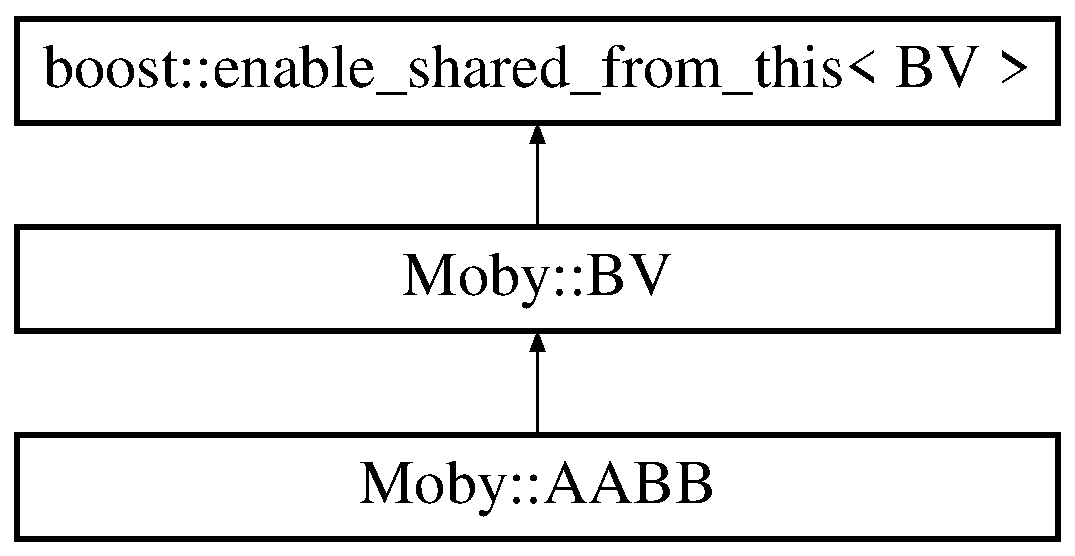
\includegraphics[height=3.000000cm]{classMoby_1_1AABB}
\end{center}
\end{figure}
\subsection*{Public Member Functions}
\begin{DoxyCompactItemize}
\item 
{\footnotesize template$<$class Input\-Iterator $>$ }\\{\bf A\-A\-B\-B} (Input\-Iterator begin, Input\-Iterator end)
\begin{DoxyCompactList}\small\item\em Constructs an axis-\/aligned bounding box using a set of points. \end{DoxyCompactList}\item 
virtual void {\bf transform} (const Ravelin\-::\-Transform3d \&T, {\bf B\-V} $\ast$result) const \label{classMoby_1_1AABB_a03f98053bf67a4aac5e804d828591e54}

\begin{DoxyCompactList}\small\item\em Transforms the \doxyref{O\-B\-B}{p.}{classMoby_1_1OBB} using the given transform. \end{DoxyCompactList}\item 
virtual bool {\bf outside} (const {\bf Point3d} \&point, double tol=N\-E\-A\-R\-\_\-\-Z\-E\-R\-O) const \label{classMoby_1_1AABB_a3f99eff66e3660da0cafcc85f8e94425}

\begin{DoxyCompactList}\small\item\em Determines whether a point is outside the bounding volume. \end{DoxyCompactList}\item 
virtual bool {\bf intersects} (const {\bf Line\-Seg3} \&seg, double \&tmin, double tmax, {\bf Point3d} \&q) const \label{classMoby_1_1AABB_ae48eec04f3ee8a8d91affda4810526e5}

\begin{DoxyCompactList}\small\item\em Determines whether a line segment intersects the bounding volume. \end{DoxyCompactList}\item 
virtual std\-::ostream \& {\bf to\-\_\-vrml} (std\-::ostream \&out, const Ravelin\-::\-Pose3d \&T) const \label{classMoby_1_1AABB_a7b4bf65c2608af7826dea5e2b2497f7f}

\begin{DoxyCompactList}\small\item\em Sends this \doxyref{A\-A\-B\-B}{p.}{classMoby_1_1AABB} to V\-R\-M\-L. \end{DoxyCompactList}\item 
virtual {\bf B\-V\-Ptr} {\bf calc\-\_\-swept\-\_\-\-B\-V} ({\bf Collision\-Geometry\-Ptr} g, const Ravelin\-::\-S\-Velocityd \&v) const \label{classMoby_1_1AABB_a975b51863c80296821a52884f8d40e85}

\begin{DoxyCompactList}\small\item\em Constructs a velocity expanded \doxyref{O\-B\-B}{p.}{classMoby_1_1OBB} using the \doxyref{A\-A\-B\-B}{p.}{classMoby_1_1AABB}. \end{DoxyCompactList}\item 
virtual double {\bf calc\-\_\-volume} () const \label{classMoby_1_1AABB_a9aa6ace140d2505be5c88f4b669cf4b5}

\begin{DoxyCompactList}\small\item\em Calculates the volume of this \doxyref{A\-A\-B\-B}{p.}{classMoby_1_1AABB}. \end{DoxyCompactList}\item 
virtual boost\-::shared\-\_\-ptr\\*
$<$ const Ravelin\-::\-Pose3d $>$ {\bf get\-\_\-relative\-\_\-pose} () const \label{classMoby_1_1AABB_a683fba20f211ced63a09b155a41b598d}

\begin{DoxyCompactList}\small\item\em Gets the associated pose for this bounding volume. \end{DoxyCompactList}\item 
virtual {\bf Point3d} {\bf get\-\_\-lower\-\_\-bounds} () const \label{classMoby_1_1AABB_a1d3f9462651e89dc4732e8cb828f3798}

\begin{DoxyCompactList}\small\item\em Gets the lower bounds for this \doxyref{A\-A\-B\-B}{p.}{classMoby_1_1AABB} using an \doxyref{O\-B\-B}{p.}{classMoby_1_1OBB}. \end{DoxyCompactList}\item 
virtual {\bf Point3d} {\bf get\-\_\-upper\-\_\-bounds} () const \label{classMoby_1_1AABB_af2e31d643dbc066d30861b2e41117935}

\begin{DoxyCompactList}\small\item\em Gets the upper bounds for this \doxyref{A\-A\-B\-B}{p.}{classMoby_1_1AABB} using an \doxyref{O\-B\-B}{p.}{classMoby_1_1OBB}. \end{DoxyCompactList}\item 
{\bf O\-B\-B} {\bf get\-\_\-\-O\-B\-B} () const \label{classMoby_1_1AABB_a43eedc052d1e5fd737f8ea80f43a0137}

\begin{DoxyCompactList}\small\item\em Gets the \doxyref{A\-A\-B\-B}{p.}{classMoby_1_1AABB} as an \doxyref{O\-B\-B}{p.}{classMoby_1_1OBB}. \end{DoxyCompactList}\item 
{\bf A\-A\-B\-B} \& {\bf operator=} (const {\bf A\-A\-B\-B} \&a)\label{classMoby_1_1AABB_ac72c2e4931b76b17ec89ceaadff6b2a6}

\begin{DoxyCompactList}\small\item\em Copies an \doxyref{A\-A\-B\-B}{p.}{classMoby_1_1AABB}. \end{DoxyCompactList}\item 
{\footnotesize template$<$class Input\-Iterator $>$ }\\{\bf A\-A\-B\-B} (Input\-Iterator begin, Input\-Iterator end)
\begin{DoxyCompactList}\small\item\em Constructs an axis-\/aligned bounding box using a set of points. \end{DoxyCompactList}\end{DoxyCompactItemize}
\subsection*{Static Public Member Functions}
\begin{DoxyCompactItemize}
\item 
static bool {\bf intersects} (const {\bf A\-A\-B\-B} \&a, const {\bf A\-A\-B\-B} \&b)\label{classMoby_1_1AABB_a5a4d81b4856b610c2a0d6e8ea074c8fd}

\begin{DoxyCompactList}\small\item\em Determines whether two A\-A\-B\-Bs overlap. \end{DoxyCompactList}\item 
static bool {\bfseries intersects} (const {\bf A\-A\-B\-B} \&a, const {\bf A\-A\-B\-B} \&b, const Ravelin\-::\-Transform3d \&a\-Tb)\label{classMoby_1_1AABB_a52cfeac2c75b96750347974c5c401e48}

\item 
static bool {\bf outside} (const {\bf A\-A\-B\-B} \&a, const {\bf Point3d} \&point, double tol=N\-E\-A\-R\-\_\-\-Z\-E\-R\-O)\label{classMoby_1_1AABB_a2e26e0b3dd1cb4f8a433fcc380204fd1}

\begin{DoxyCompactList}\small\item\em Determines whether a point is outside of a \doxyref{A\-A\-B\-B}{p.}{classMoby_1_1AABB}. \end{DoxyCompactList}\item 
static bool {\bf intersects} (const {\bf A\-A\-B\-B} \&a, const {\bf Line\-Seg3} \&seg, double \&tmin, double tmax, {\bf Point3d} \&q)
\begin{DoxyCompactList}\small\item\em Determines whether an \doxyref{O\-B\-B}{p.}{classMoby_1_1OBB} and a line/ray/line segment intersect. \end{DoxyCompactList}\item 
static void {\bf get\-\_\-closest\-\_\-point} (const {\bf A\-A\-B\-B} \&a, const {\bf Point3d} \&p, {\bf Point3d} \&closest)\label{classMoby_1_1AABB_ae3162ae0fe017ae9551c65a2522b352f}

\begin{DoxyCompactList}\small\item\em Gets the closest point on the \doxyref{A\-A\-B\-B}{p.}{classMoby_1_1AABB} to a point. \end{DoxyCompactList}\item 
static double {\bf get\-\_\-farthest\-\_\-point} (const {\bf A\-A\-B\-B} \&a, const {\bf Point3d} \&p, {\bf Point3d} \&farthest)
\begin{DoxyCompactList}\small\item\em Gets the farthest point on the \doxyref{A\-A\-B\-B}{p.}{classMoby_1_1AABB} to a point. \end{DoxyCompactList}\end{DoxyCompactItemize}
\subsection*{Public Attributes}
\begin{DoxyCompactItemize}
\item 
{\bf Point3d} {\bf minp}\label{classMoby_1_1AABB_a23122d7eb40203c799bda7927614f169}

\begin{DoxyCompactList}\small\item\em The lower corner of the \doxyref{A\-A\-B\-B}{p.}{classMoby_1_1AABB}. \end{DoxyCompactList}\item 
{\bf Point3d} {\bf maxp}\label{classMoby_1_1AABB_a40136d928f575e010ca33c433bdbc937}

\begin{DoxyCompactList}\small\item\em The upper corner of the \doxyref{A\-A\-B\-B}{p.}{classMoby_1_1AABB};. \end{DoxyCompactList}\end{DoxyCompactItemize}


\subsection{Detailed Description}
An axis-\/aligned bounding box. 

\subsection{Constructor \& Destructor Documentation}
\index{Moby\-::\-A\-A\-B\-B@{Moby\-::\-A\-A\-B\-B}!A\-A\-B\-B@{A\-A\-B\-B}}
\index{A\-A\-B\-B@{A\-A\-B\-B}!Moby::AABB@{Moby\-::\-A\-A\-B\-B}}
\subsubsection[{A\-A\-B\-B}]{\setlength{\rightskip}{0pt plus 5cm}template$<$class Input\-Iterator $>$ Moby\-::\-A\-A\-B\-B\-::\-A\-A\-B\-B (
\begin{DoxyParamCaption}
\item[{Input\-Iterator}]{begin, }
\item[{Input\-Iterator}]{end}
\end{DoxyParamCaption}
)}\label{classMoby_1_1AABB_a57b09622e67c481ff53fc3c8f3cd4a04}


Constructs an axis-\/aligned bounding box using a set of points. 


\begin{DoxyParams}{Parameters}
{\em begin} & an iterator to the beginning of a container of type Ravelin\-::\-Vector3 \\
\hline
{\em end} & an iterator to the end of a container of type Ravelin\-::\-Vector3 \\
\hline
\end{DoxyParams}
\index{Moby\-::\-A\-A\-B\-B@{Moby\-::\-A\-A\-B\-B}!A\-A\-B\-B@{A\-A\-B\-B}}
\index{A\-A\-B\-B@{A\-A\-B\-B}!Moby::AABB@{Moby\-::\-A\-A\-B\-B}}
\subsubsection[{A\-A\-B\-B}]{\setlength{\rightskip}{0pt plus 5cm}template$<$class Input\-Iterator $>$ Moby\-::\-A\-A\-B\-B\-::\-A\-A\-B\-B (
\begin{DoxyParamCaption}
\item[{Input\-Iterator}]{begin, }
\item[{Input\-Iterator}]{end}
\end{DoxyParamCaption}
)}\label{classMoby_1_1AABB_a57b09622e67c481ff53fc3c8f3cd4a04}


Constructs an axis-\/aligned bounding box using a set of points. 


\begin{DoxyParams}{Parameters}
{\em begin} & an iterator to the beginning of a container of type Ravelin\-::\-Vector3 \\
\hline
{\em end} & an iterator to the end of a container of type Ravelin\-::\-Vector3 \\
\hline
\end{DoxyParams}


\subsection{Member Function Documentation}
\index{Moby\-::\-A\-A\-B\-B@{Moby\-::\-A\-A\-B\-B}!get\-\_\-farthest\-\_\-point@{get\-\_\-farthest\-\_\-point}}
\index{get\-\_\-farthest\-\_\-point@{get\-\_\-farthest\-\_\-point}!Moby::AABB@{Moby\-::\-A\-A\-B\-B}}
\subsubsection[{get\-\_\-farthest\-\_\-point}]{\setlength{\rightskip}{0pt plus 5cm}double A\-A\-B\-B\-::get\-\_\-farthest\-\_\-point (
\begin{DoxyParamCaption}
\item[{const {\bf A\-A\-B\-B} \&}]{a, }
\item[{const {\bf Point3d} \&}]{p, }
\item[{{\bf Point3d} \&}]{farthest}
\end{DoxyParamCaption}
)\hspace{0.3cm}{\ttfamily [static]}}\label{classMoby_1_1AABB_a6d7abe8db78eb3f367871a664be2321a}


Gets the farthest point on the \doxyref{A\-A\-B\-B}{p.}{classMoby_1_1AABB} to a point. 

Returns the squared distance to the farthest point 

References get\-\_\-relative\-\_\-pose(), maxp, and minp.

\index{Moby\-::\-A\-A\-B\-B@{Moby\-::\-A\-A\-B\-B}!intersects@{intersects}}
\index{intersects@{intersects}!Moby::AABB@{Moby\-::\-A\-A\-B\-B}}
\subsubsection[{intersects}]{\setlength{\rightskip}{0pt plus 5cm}bool A\-A\-B\-B\-::intersects (
\begin{DoxyParamCaption}
\item[{const {\bf A\-A\-B\-B} \&}]{a, }
\item[{const {\bf Line\-Seg3} \&}]{seg, }
\item[{double \&}]{tmin, }
\item[{double}]{tmax, }
\item[{{\bf Point3d} \&}]{q}
\end{DoxyParamCaption}
)\hspace{0.3cm}{\ttfamily [static]}}\label{classMoby_1_1AABB_a0ea4ddc787863ffc46540149cc6f9472}


Determines whether an \doxyref{O\-B\-B}{p.}{classMoby_1_1OBB} and a line/ray/line segment intersect. 

When intersecting, return intersection distance tmin and point q of intersection. 
\begin{DoxyParams}{Parameters}
{\em a} & the \doxyref{O\-B\-B}{p.}{classMoby_1_1OBB} to check for intersection \\
\hline
{\em seg} & the line segment to check for intersection \\
\hline
{\em tmin} & on entry, contains the minimum value of the line parameter-\/ for a line segment, this will generally be 0; when an intersection occurs, this will contain the distance of intersection from the tmin that was input on return \\
\hline
{\em tmax} & the maximum value of the line parameter-\/ for a line segment, this will generally be 1 \\
\hline
{\em q} & contains the point of intersection, if any, on return \\
\hline
\end{DoxyParams}
\begin{DoxyReturn}{Returns}
{\bfseries true} if the \doxyref{O\-B\-B}{p.}{classMoby_1_1OBB} and line intersect, {\bfseries false} otherwise 
\end{DoxyReturn}
\begin{DoxyNote}{Note}
code adapted from [Ericson, 2005], pp. 180-\/181 
\end{DoxyNote}


References maxp, and minp.



The documentation for this class was generated from the following files\-:\begin{DoxyCompactItemize}
\item 
/home/drum/\-Moby/include/\-Moby/A\-A\-B\-B.\-h\item 
/home/drum/\-Moby/include/\-Moby/A\-A\-B\-B.\-inl\item 
/home/drum/\-Moby/src/A\-A\-B\-B.\-cpp\end{DoxyCompactItemize}

\section{Moby\-:\-:Articulated\-Body Class Reference}
\label{classMoby_1_1ArticulatedBody}\index{Moby\-::\-Articulated\-Body@{Moby\-::\-Articulated\-Body}}


Abstract class for articulated bodies.  




{\ttfamily \#include $<$Articulated\-Body.\-h$>$}

Inheritance diagram for Moby\-:\-:Articulated\-Body\-:\begin{figure}[H]
\begin{center}
\leavevmode
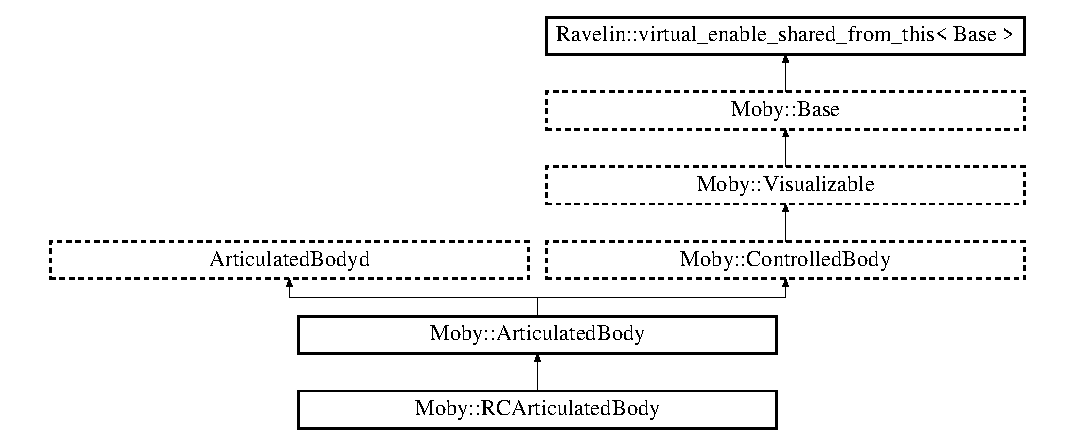
\includegraphics[height=5.526316cm]{classMoby_1_1ArticulatedBody}
\end{center}
\end{figure}
\subsection*{Public Member Functions}
\begin{DoxyCompactItemize}
\item 
virtual void {\bf update\-\_\-visualization} ()\label{classMoby_1_1ArticulatedBody_a25e7ceab132042083e42c97d202d7f72}

\begin{DoxyCompactList}\small\item\em Updates visualization for the body. \end{DoxyCompactList}\item 
virtual void {\bf load\-\_\-from\-\_\-xml} (boost\-::shared\-\_\-ptr$<$ const {\bf X\-M\-L\-Tree} $>$ node, std\-::map$<$ std\-::string, {\bf Base\-Ptr} $>$ \&id\-\_\-map)\label{classMoby_1_1ArticulatedBody_a7d86b8e81bee372ba5cd5de35ccfde59}

\begin{DoxyCompactList}\small\item\em Loads a M\-C\-Articulated\-Body object from an X\-M\-L node. \end{DoxyCompactList}\item 
virtual void {\bf save\-\_\-to\-\_\-xml} ({\bf X\-M\-L\-Tree\-Ptr} node, std\-::list$<$ boost\-::shared\-\_\-ptr$<$ const {\bf Base} $>$ $>$ \&shared\-\_\-objects) const \label{classMoby_1_1ArticulatedBody_a7575e65e7721f2f2f10b1d83c18c50e1}

\begin{DoxyCompactList}\small\item\em Saves this object to a X\-M\-L tree. \end{DoxyCompactList}\item 
void {\bf update\-\_\-joint\-\_\-constraint\-\_\-violations} ()\label{classMoby_1_1ArticulatedBody_ab8ddbc9ebb0c4bea926e20db703962dd}

\begin{DoxyCompactList}\small\item\em Updates joint constraint violation (after integration) \end{DoxyCompactList}\item 
bool {\bf is\-\_\-joint\-\_\-constraint\-\_\-violated} () const \label{classMoby_1_1ArticulatedBody_a9cef68d126a420e21cad2be2f201b6a1}

\begin{DoxyCompactList}\small\item\em Checks for a joint constraint violation. \end{DoxyCompactList}\item 
virtual void {\bf prepare\-\_\-to\-\_\-calc\-\_\-ode} (Ravelin\-::\-Shared\-Const\-Vector\-Nd \&x, double t, double dt, void $\ast$data)\label{classMoby_1_1ArticulatedBody_aee3394378fd462a5e26693963bd284db}

\begin{DoxyCompactList}\small\item\em Prepares to compute the O\-D\-E. \end{DoxyCompactList}\item 
virtual void {\bf prepare\-\_\-to\-\_\-calc\-\_\-ode\-\_\-sustained\-\_\-constraints} (Ravelin\-::\-Shared\-Const\-Vector\-Nd \&x, double t, double dt, void $\ast$data)
\begin{DoxyCompactList}\small\item\em Integrates a dynamic body. \end{DoxyCompactList}\item 
virtual void {\bf ode} (double t, double dt, void $\ast$data, Ravelin\-::\-Shared\-Vector\-Nd \&dx)\label{classMoby_1_1ArticulatedBody_ac63d7eb817824cd6950cf99dd8639099}

\begin{DoxyCompactList}\small\item\em Returns the O\-D\-E's for position and velocity (concatenated into x) \end{DoxyCompactList}\item 
{\footnotesize template$<$class Output\-Iterator $>$ }\\Output\-Iterator {\bf find\-\_\-limit\-\_\-constraints} (Output\-Iterator begin) const 
\begin{DoxyCompactList}\small\item\em Finds (joint) limit constraints. \end{DoxyCompactList}\item 
{\bf Articulated\-Body\-Ptr} {\bf get\-\_\-this} ()\label{classMoby_1_1ArticulatedBody_ac61a241230348acc8ce3d89e4205cb64}

\begin{DoxyCompactList}\small\item\em Gets shared pointer to this object as type \doxyref{Articulated\-Body}{p.}{classMoby_1_1ArticulatedBody}. \end{DoxyCompactList}\item 
boost\-::shared\-\_\-ptr$<$ const \\*
{\bf Articulated\-Body} $>$ {\bf get\-\_\-this} () const \label{classMoby_1_1ArticulatedBody_aa5157709347a4a5825ea37118388675d}

\begin{DoxyCompactList}\small\item\em Gets shared pointer to this object as type const Articulate\-Body. \end{DoxyCompactList}\item 
{\footnotesize template$<$class Output\-Iterator $>$ }\\Output\-Iterator {\bf find\-\_\-limit\-\_\-constraints} (Output\-Iterator output\-\_\-begin) const \label{classMoby_1_1ArticulatedBody_accfe42433b3a6f9877c73b306756263f}

\begin{DoxyCompactList}\small\item\em Gets joint limit constraints. \end{DoxyCompactList}\end{DoxyCompactItemize}
\subsection*{Additional Inherited Members}


\subsection{Detailed Description}
Abstract class for articulated bodies. 

\subsection{Member Function Documentation}
\index{Moby\-::\-Articulated\-Body@{Moby\-::\-Articulated\-Body}!find\-\_\-limit\-\_\-constraints@{find\-\_\-limit\-\_\-constraints}}
\index{find\-\_\-limit\-\_\-constraints@{find\-\_\-limit\-\_\-constraints}!Moby::ArticulatedBody@{Moby\-::\-Articulated\-Body}}
\subsubsection[{find\-\_\-limit\-\_\-constraints}]{\setlength{\rightskip}{0pt plus 5cm}template$<$class Output\-Iterator $>$ Output\-Iterator Moby\-::\-Articulated\-Body\-::find\-\_\-limit\-\_\-constraints (
\begin{DoxyParamCaption}
\item[{Output\-Iterator}]{begin}
\end{DoxyParamCaption}
) const}\label{classMoby_1_1ArticulatedBody_acdffb965a0b6aa6143b9b3a0b9ec1452}


Finds (joint) limit constraints. 

Gets joint limit constraints. 

Referenced by Moby\-::\-Constraint\-Simulator\-::find\-\_\-unilateral\-\_\-constraints().

\index{Moby\-::\-Articulated\-Body@{Moby\-::\-Articulated\-Body}!prepare\-\_\-to\-\_\-calc\-\_\-ode\-\_\-sustained\-\_\-constraints@{prepare\-\_\-to\-\_\-calc\-\_\-ode\-\_\-sustained\-\_\-constraints}}
\index{prepare\-\_\-to\-\_\-calc\-\_\-ode\-\_\-sustained\-\_\-constraints@{prepare\-\_\-to\-\_\-calc\-\_\-ode\-\_\-sustained\-\_\-constraints}!Moby::ArticulatedBody@{Moby\-::\-Articulated\-Body}}
\subsubsection[{prepare\-\_\-to\-\_\-calc\-\_\-ode\-\_\-sustained\-\_\-constraints}]{\setlength{\rightskip}{0pt plus 5cm}void Articulated\-Body\-::prepare\-\_\-to\-\_\-calc\-\_\-ode\-\_\-sustained\-\_\-constraints (
\begin{DoxyParamCaption}
\item[{Ravelin\-::\-Shared\-Const\-Vector\-Nd \&}]{x, }
\item[{double}]{t, }
\item[{double}]{dt, }
\item[{void $\ast$}]{data}
\end{DoxyParamCaption}
)\hspace{0.3cm}{\ttfamily [virtual]}}\label{classMoby_1_1ArticulatedBody_afb57aa1ffee8c64fb1a829b1ad2124c6}


Integrates a dynamic body. 

Prepares to compute the O\-D\-E 

Implements {\bf Moby\-::\-Controlled\-Body} \doxyref{}{p.}{classMoby_1_1ControlledBody_a6df8a844762bcc3cacd27b21e1e3b0c9}.



The documentation for this class was generated from the following files\-:\begin{DoxyCompactItemize}
\item 
/home/drum/\-Moby/include/\-Moby/Articulated\-Body.\-h\item 
/home/drum/\-Moby/include/\-Moby/Articulated\-Body.\-inl\item 
/home/drum/\-Moby/src/Articulated\-Body.\-cpp\end{DoxyCompactItemize}

\section{Moby\-:\-:Base Class Reference}
\label{classMoby_1_1Base}\index{Moby\-::\-Base@{Moby\-::\-Base}}


Class from which all \doxyref{Moby}{p.}{namespaceMoby} classes are derived.  




{\ttfamily \#include $<$Base.\-h$>$}

Inheritance diagram for Moby\-:\-:Base\-:\begin{figure}[H]
\begin{center}
\leavevmode
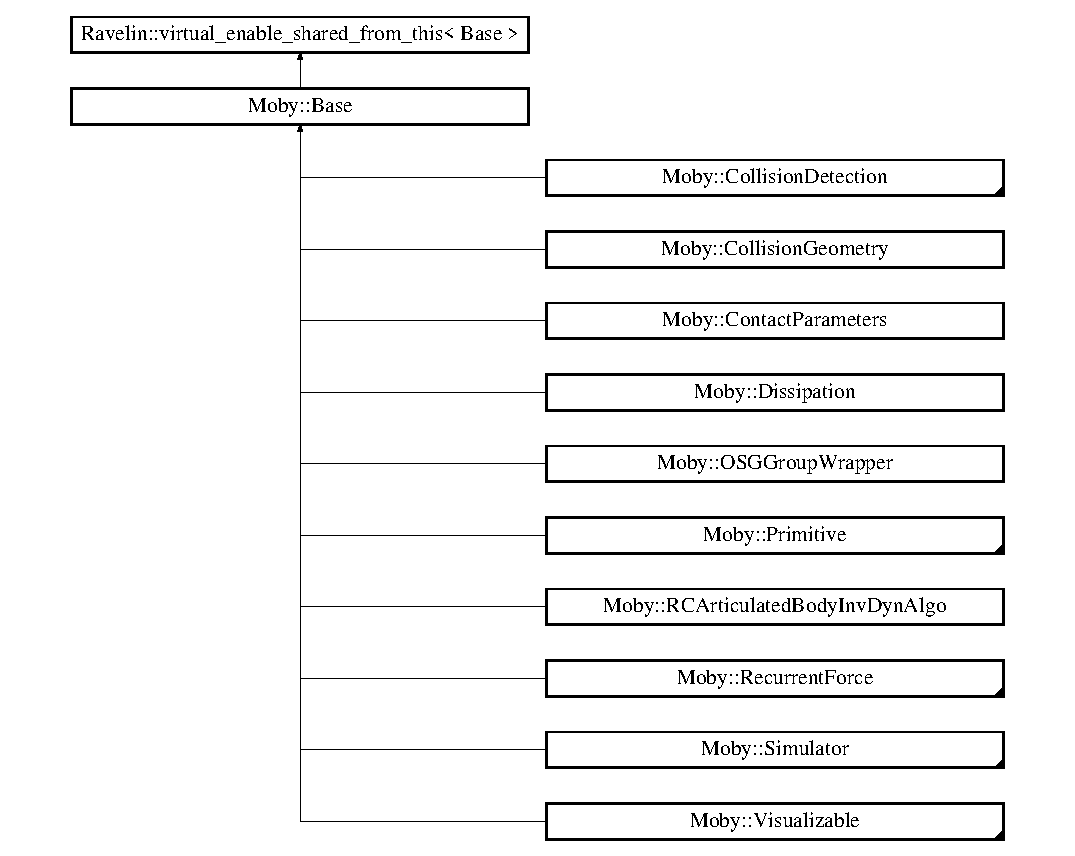
\includegraphics[height=11.052631cm]{classMoby_1_1Base}
\end{center}
\end{figure}
\subsection*{Public Member Functions}
\begin{DoxyCompactItemize}
\item 
{\bfseries Base} (const {\bf Base} $\ast$b)\label{classMoby_1_1Base_a206ffc0f68275eb1675dc4311fc9ec02}

\item 
virtual void {\bf save\-\_\-to\-\_\-xml} ({\bf X\-M\-L\-Tree\-Ptr} node, std\-::list$<$ boost\-::shared\-\_\-ptr$<$ const {\bf Base} $>$ $>$ \&shared\-\_\-objects) const 
\begin{DoxyCompactList}\small\item\em Method for saving this object to X\-M\-L. \end{DoxyCompactList}\item 
virtual void {\bf load\-\_\-from\-\_\-xml} (boost\-::shared\-\_\-ptr$<$ const {\bf X\-M\-L\-Tree} $>$ node, std\-::map$<$ std\-::string, {\bf Base\-Ptr} $>$ \&id\-\_\-map)
\begin{DoxyCompactList}\small\item\em Method for loading the data for this object from X\-M\-L. \end{DoxyCompactList}\end{DoxyCompactItemize}
\subsection*{Static Public Member Functions}
\begin{DoxyCompactItemize}
\item 
{\footnotesize template$<$class T $>$ }\\static boost\-::shared\-\_\-ptr$<$ T $>$ {\bf clone} (boost\-::shared\-\_\-ptr$<$ T $>$ x)\label{classMoby_1_1Base_a5283a4b27f562f9d8db6a9f320919fc5}

\begin{DoxyCompactList}\small\item\em Static method for cloning a shared pointer. \end{DoxyCompactList}\end{DoxyCompactItemize}
\subsection*{Public Attributes}
\begin{DoxyCompactItemize}
\item 
boost\-::shared\-\_\-ptr$<$ void $>$ {\bf userdata}\label{classMoby_1_1Base_a88ad4f992e3b86c9963835cc0999f66e}

\begin{DoxyCompactList}\small\item\em Any relevant userdata. \end{DoxyCompactList}\item 
std\-::string {\bf id}\label{classMoby_1_1Base_a1ffc84e8895c67e1010dd34d50244cf7}

\begin{DoxyCompactList}\small\item\em The unique I\-D for this object. \end{DoxyCompactList}\end{DoxyCompactItemize}


\subsection{Detailed Description}
Class from which all \doxyref{Moby}{p.}{namespaceMoby} classes are derived. 

\subsection{Member Function Documentation}
\index{Moby\-::\-Base@{Moby\-::\-Base}!load\-\_\-from\-\_\-xml@{load\-\_\-from\-\_\-xml}}
\index{load\-\_\-from\-\_\-xml@{load\-\_\-from\-\_\-xml}!Moby::Base@{Moby\-::\-Base}}
\subsubsection[{load\-\_\-from\-\_\-xml}]{\setlength{\rightskip}{0pt plus 5cm}void Base\-::load\-\_\-from\-\_\-xml (
\begin{DoxyParamCaption}
\item[{boost\-::shared\-\_\-ptr$<$ const {\bf X\-M\-L\-Tree} $>$}]{node, }
\item[{std\-::map$<$ std\-::string, {\bf Base\-Ptr} $>$ \&}]{id\-\_\-map}
\end{DoxyParamCaption}
)\hspace{0.3cm}{\ttfamily [virtual]}}\label{classMoby_1_1Base_a98b861c1d615a748b576aa613f17389f}


Method for loading the data for this object from X\-M\-L. 


\begin{DoxyParams}{Parameters}
{\em node} & the subtree under which all data necessary to load this object is stored \\
\hline
{\em id\-\_\-map} & a map from node I\-Ds to read objects \\
\hline
\end{DoxyParams}


Reimplemented in {\bf Moby\-::\-Rigid\-Body} \doxyref{}{p.}{classMoby_1_1RigidBody_a26bee5f435e488d8048e0b827ee91004}, {\bf Moby\-::\-Simulator} \doxyref{}{p.}{classMoby_1_1Simulator_a8fc61be0cf1e142e0ce9c188eb5b0871}, {\bf Moby\-::\-R\-C\-Articulated\-Body} \doxyref{}{p.}{classMoby_1_1RCArticulatedBody_a8e694464f29ac406b4b9ecef5e0d8bac}, {\bf Moby\-::\-Primitive} \doxyref{}{p.}{classMoby_1_1Primitive_ab2cb5a7043032a8a3df736909740d1f7}, {\bf Moby\-::\-Joint} \doxyref{}{p.}{classMoby_1_1Joint_a5e0c23575a509a152d212b2b7dc3ffa6}, {\bf Moby\-::\-Collision\-Geometry} \doxyref{}{p.}{classMoby_1_1CollisionGeometry_a164759946c1a08773bc6bea03c3008c8}, {\bf Moby\-::\-Plane\-Primitive} \doxyref{}{p.}{classMoby_1_1PlanePrimitive_ac8093c3e57621aab0884ae91b1e37f5d}, {\bf Moby\-::\-Visualizable} \doxyref{}{p.}{classMoby_1_1Visualizable_a8d9fc36646c0df143c99c488740edfbb}, {\bf Moby\-::\-C\-C\-D} \doxyref{}{p.}{classMoby_1_1CCD_ac2537ed877fb1303bcef42fe372e61d5}, {\bf Moby\-::\-Gears} \doxyref{}{p.}{classMoby_1_1Gears_a5e7fe5c59b73c07c727715640f067dfb}, {\bf Moby\-::\-Heightmap\-Primitive} \doxyref{}{p.}{classMoby_1_1HeightmapPrimitive_acbe882c1a5fd97b2537a0cbab860e8a4}, {\bf Moby\-::\-Constraint\-Simulator} \doxyref{}{p.}{classMoby_1_1ConstraintSimulator_aea925f7a62d28833ec377e7176bcca78}, {\bf Moby\-::\-Polyhedral\-Primitive} \doxyref{}{p.}{classMoby_1_1PolyhedralPrimitive_a54ede66e39b6ae57827a6cbeb9480335}, {\bf Moby\-::\-Triangle\-Mesh\-Primitive} \doxyref{}{p.}{classMoby_1_1TriangleMeshPrimitive_a568de88a674606645f2b980729469aef}, {\bf Moby\-::\-Cone\-Primitive} \doxyref{}{p.}{classMoby_1_1ConePrimitive_a5fb7ad4ce31f041a8933cb67e30c3c8b}, {\bf Moby\-::\-Time\-Stepping\-Simulator} \doxyref{}{p.}{classMoby_1_1TimeSteppingSimulator_a1b29397680cc9ca652eaf790b77d0191}, {\bf Moby\-::\-Controlled\-Body} \doxyref{}{p.}{classMoby_1_1ControlledBody_aa537fd1b68d720745cd7a7a2580ce9d3}, {\bf Moby\-::\-Articulated\-Body} \doxyref{}{p.}{classMoby_1_1ArticulatedBody_a7d86b8e81bee372ba5cd5de35ccfde59}, {\bf Moby\-::\-Cylinder\-Primitive} \doxyref{}{p.}{classMoby_1_1CylinderPrimitive_a8530fa4d6370204c5333e0fe73a570df}, {\bf Moby\-::\-Prismatic\-Joint} \doxyref{}{p.}{classMoby_1_1PrismaticJoint_a32fce63f6af0d1508aeb741941f58996}, {\bf Moby\-::\-Box\-Primitive} \doxyref{}{p.}{classMoby_1_1BoxPrimitive_a3d40e1f701caccca8fbdf8cbc473b788}, {\bf Moby\-::\-Sphere\-Primitive} \doxyref{}{p.}{classMoby_1_1SpherePrimitive_abf18dff5adc902467124296cc2972e20}, {\bf Moby\-::\-Fixed\-Joint} \doxyref{}{p.}{classMoby_1_1FixedJoint_a02e637422d026f869ab138b3c76de654}, {\bf Moby\-::\-O\-S\-G\-Group\-Wrapper} \doxyref{}{p.}{classMoby_1_1OSGGroupWrapper_a9d5827d7a78065b9bc376d90e0bac2f9}, {\bf Moby\-::\-Planar\-Joint} \doxyref{}{p.}{classMoby_1_1PlanarJoint_abc73fa718eff71b90bbd0ce4ba92106d}, {\bf Moby\-::\-Revolute\-Joint} \doxyref{}{p.}{classMoby_1_1RevoluteJoint_af72df350d32e71d76b3505f29a633cce}, {\bf Moby\-::\-Spherical\-Joint} \doxyref{}{p.}{classMoby_1_1SphericalJoint_a34675294343bd4326dd20d404476fcd6}, {\bf Moby\-::\-Universal\-Joint} \doxyref{}{p.}{classMoby_1_1UniversalJoint_a5fb810551da607d8bc8288e7c0e49f4d}, {\bf Moby\-::\-Screw\-Joint} \doxyref{}{p.}{classMoby_1_1ScrewJoint_a6fd5ddb252a077e791697bc90718ab5d}, {\bf Moby\-::\-Torus\-Primitive} \doxyref{}{p.}{classMoby_1_1TorusPrimitive_af9259af65850343c7df49053a9e5a692}, {\bf Moby\-::\-Gravity\-Force} \doxyref{}{p.}{classMoby_1_1GravityForce_a61d8468de9c5bc8d2a8853bec08d14fe}, {\bf Moby\-::\-Contact\-Parameters} \doxyref{}{p.}{classMoby_1_1ContactParameters_a00c9c5d4c9c1f9a5f8235689de2c590d}, {\bf Moby\-::\-Stokes\-Drag\-Force} \doxyref{}{p.}{classMoby_1_1StokesDragForce_aa89874941cd4860ff97d8ea0cb3af524}, and {\bf Moby\-::\-Dissipation} \doxyref{}{p.}{classMoby_1_1Dissipation_ac029254a743326952f34aa8ce21b1477}.



References id.

\index{Moby\-::\-Base@{Moby\-::\-Base}!save\-\_\-to\-\_\-xml@{save\-\_\-to\-\_\-xml}}
\index{save\-\_\-to\-\_\-xml@{save\-\_\-to\-\_\-xml}!Moby::Base@{Moby\-::\-Base}}
\subsubsection[{save\-\_\-to\-\_\-xml}]{\setlength{\rightskip}{0pt plus 5cm}void Base\-::save\-\_\-to\-\_\-xml (
\begin{DoxyParamCaption}
\item[{{\bf X\-M\-L\-Tree\-Ptr}}]{node, }
\item[{std\-::list$<$ boost\-::shared\-\_\-ptr$<$ const {\bf Base} $>$ $>$ \&}]{shared\-\_\-objects}
\end{DoxyParamCaption}
) const\hspace{0.3cm}{\ttfamily [virtual]}}\label{classMoby_1_1Base_aed64905ca39893d02d1e6c3f03f73aa9}


Method for saving this object to X\-M\-L. 


\begin{DoxyParams}{Parameters}
{\em node} & the X\-M\-L node to which this object should be serialized \\
\hline
{\em on} & output, a list of shared objects which should also be serialized \\
\hline
\end{DoxyParams}


Reimplemented in {\bf Moby\-::\-Rigid\-Body} \doxyref{}{p.}{classMoby_1_1RigidBody_a071ed106863e0cd018b5ccf3bce5f5e2}, {\bf Moby\-::\-Simulator} \doxyref{}{p.}{classMoby_1_1Simulator_a95b0ea5486c10f5c80d088e85f330b12}, {\bf Moby\-::\-R\-C\-Articulated\-Body} \doxyref{}{p.}{classMoby_1_1RCArticulatedBody_a08ce8cf881fda06a41bb2323da25f802}, {\bf Moby\-::\-Primitive} \doxyref{}{p.}{classMoby_1_1Primitive_aa5925c970e939796f5fd07d1c8198437}, {\bf Moby\-::\-Joint} \doxyref{}{p.}{classMoby_1_1Joint_ab5ad56ab0008dfd54a78aa3289854af7}, {\bf Moby\-::\-Collision\-Geometry} \doxyref{}{p.}{classMoby_1_1CollisionGeometry_a22ac18e99fa56f198d91faecf8b7f8e1}, {\bf Moby\-::\-Plane\-Primitive} \doxyref{}{p.}{classMoby_1_1PlanePrimitive_a860a58e5f0a52e8b6a6c94996e0886d6}, {\bf Moby\-::\-C\-C\-D} \doxyref{}{p.}{classMoby_1_1CCD_a9c3cf2fc9e7827ba8bcb584cf2dba31b}, {\bf Moby\-::\-Visualizable} \doxyref{}{p.}{classMoby_1_1Visualizable_a758e48d853b6bb2085c98f1d5438cf5c}, {\bf Moby\-::\-Heightmap\-Primitive} \doxyref{}{p.}{classMoby_1_1HeightmapPrimitive_a36f1a53d9a69a39f944ff1462ef161b6}, {\bf Moby\-::\-Constraint\-Simulator} \doxyref{}{p.}{classMoby_1_1ConstraintSimulator_aa97902317a931eb41b6e67069aa3c236}, {\bf Moby\-::\-Polyhedral\-Primitive} \doxyref{}{p.}{classMoby_1_1PolyhedralPrimitive_a2c023ea6208e9817586997ac753d506e}, {\bf Moby\-::\-Gears} \doxyref{}{p.}{classMoby_1_1Gears_a9aa0d3984cc06b49b42bccfe6e86f4dd}, {\bf Moby\-::\-Triangle\-Mesh\-Primitive} \doxyref{}{p.}{classMoby_1_1TriangleMeshPrimitive_a12bc7caf20ec07e992a37ffd313812d4}, {\bf Moby\-::\-Cone\-Primitive} \doxyref{}{p.}{classMoby_1_1ConePrimitive_a7cf26ee13c1fe73f766d7dba07b55cda}, {\bf Moby\-::\-Time\-Stepping\-Simulator} \doxyref{}{p.}{classMoby_1_1TimeSteppingSimulator_a9fbe88f409947ebdec530bf0d221182c}, {\bf Moby\-::\-Controlled\-Body} \doxyref{}{p.}{classMoby_1_1ControlledBody_a8652ca9cedf67ee84f29ea004bb1a872}, {\bf Moby\-::\-Articulated\-Body} \doxyref{}{p.}{classMoby_1_1ArticulatedBody_a7575e65e7721f2f2f10b1d83c18c50e1}, {\bf Moby\-::\-Cylinder\-Primitive} \doxyref{}{p.}{classMoby_1_1CylinderPrimitive_acd5e18cdf754052894557d7c84719dfd}, {\bf Moby\-::\-Prismatic\-Joint} \doxyref{}{p.}{classMoby_1_1PrismaticJoint_ac5d2ef542aa70f2efe38b59cfade8ced}, {\bf Moby\-::\-Box\-Primitive} \doxyref{}{p.}{classMoby_1_1BoxPrimitive_a7567d7f558da7d8ee30993edb465e8ab}, {\bf Moby\-::\-Sphere\-Primitive} \doxyref{}{p.}{classMoby_1_1SpherePrimitive_a153f43c1030cb7a64f40b316870aac8f}, {\bf Moby\-::\-Fixed\-Joint} \doxyref{}{p.}{classMoby_1_1FixedJoint_abd170c47b08339efdc26ea5929aea3a3}, {\bf Moby\-::\-O\-S\-G\-Group\-Wrapper} \doxyref{}{p.}{classMoby_1_1OSGGroupWrapper_ae407d4e31677c2516bd5ed795de535f7}, {\bf Moby\-::\-Planar\-Joint} \doxyref{}{p.}{classMoby_1_1PlanarJoint_a3614b2d0ff84262b8eb3656320e484a1}, {\bf Moby\-::\-Revolute\-Joint} \doxyref{}{p.}{classMoby_1_1RevoluteJoint_a97b43695c74e98937997e30f71b3b26d}, {\bf Moby\-::\-Spherical\-Joint} \doxyref{}{p.}{classMoby_1_1SphericalJoint_a620cb80de5502c45583e7c74ebfa7ba1}, {\bf Moby\-::\-Universal\-Joint} \doxyref{}{p.}{classMoby_1_1UniversalJoint_adce87f1eaaaa7ae81825d5e062060076}, {\bf Moby\-::\-Screw\-Joint} \doxyref{}{p.}{classMoby_1_1ScrewJoint_a3310bc567f4fa3a82bae87d5d35dcffb}, {\bf Moby\-::\-Torus\-Primitive} \doxyref{}{p.}{classMoby_1_1TorusPrimitive_a61fa62d907b90f00b78a66bb7b62af91}, {\bf Moby\-::\-Gravity\-Force} \doxyref{}{p.}{classMoby_1_1GravityForce_af3d2dc707d49572209c0b24105cecc98}, {\bf Moby\-::\-Contact\-Parameters} \doxyref{}{p.}{classMoby_1_1ContactParameters_aaa6f5a2f71dab3cb2a2bfd750d8ba0f2}, {\bf Moby\-::\-Stokes\-Drag\-Force} \doxyref{}{p.}{classMoby_1_1StokesDragForce_a0b072b877cff16bee5113d1fecbeccaa}, and {\bf Moby\-::\-Dissipation} \doxyref{}{p.}{classMoby_1_1Dissipation_ad064eff747616a8cd13d6385c49f4ff7}.



The documentation for this class was generated from the following files\-:\begin{DoxyCompactItemize}
\item 
/home/drum/\-Moby/include/\-Moby/Base.\-h\item 
/home/drum/\-Moby/src/Base.\-cpp\end{DoxyCompactItemize}

\section{Moby\-:\-:Base\-Data Class Reference}
\label{classMoby_1_1BaseData}\index{Moby\-::\-Base\-Data@{Moby\-::\-Base\-Data}}
\subsection*{Public Member Functions}
\begin{DoxyCompactItemize}
\item 
{\bfseries Base\-Data} (const {\bf Base} $\ast$b)\label{classMoby_1_1BaseData_a594764afb4eddddf3395f9fb369a50bf}

\item 
void {\bfseries populate} ({\bf Base} $\ast$b)\label{classMoby_1_1BaseData_abcfb4838b9f9b5f7cd739bafbc3b125a}

\end{DoxyCompactItemize}


The documentation for this class was generated from the following file\-:\begin{DoxyCompactItemize}
\item 
/home/drum/\-Moby/src/Base.\-cpp\end{DoxyCompactItemize}

\section{Moby\-:\-:Bounding\-Sphere Class Reference}
\label{classMoby_1_1BoundingSphere}\index{Moby\-::\-Bounding\-Sphere@{Moby\-::\-Bounding\-Sphere}}


A sphere used for bounding geometry.  




{\ttfamily \#include $<$Bounding\-Sphere.\-h$>$}

Inheritance diagram for Moby\-:\-:Bounding\-Sphere\-:\begin{figure}[H]
\begin{center}
\leavevmode
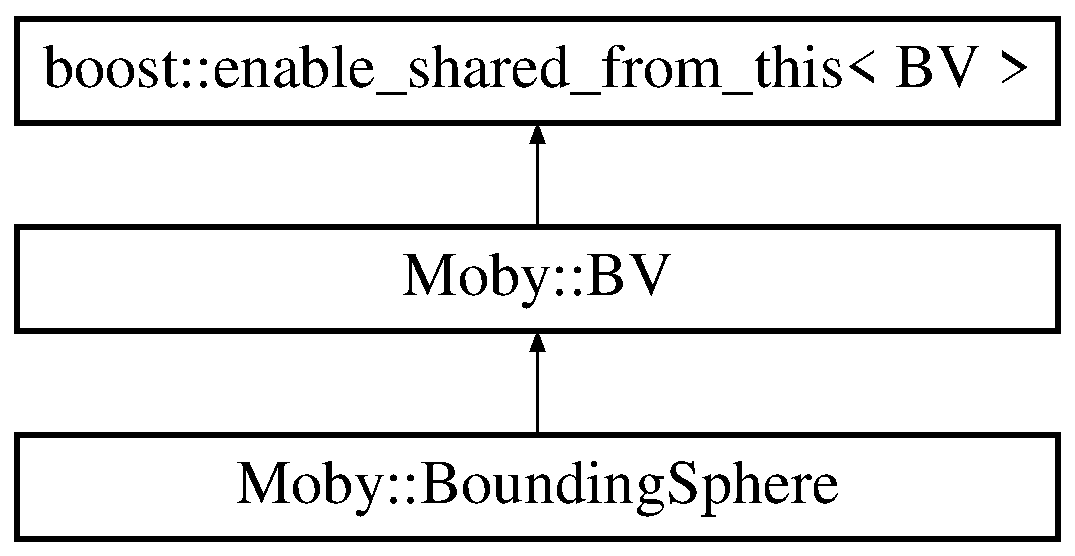
\includegraphics[height=3.000000cm]{classMoby_1_1BoundingSphere}
\end{center}
\end{figure}
\subsection*{Public Member Functions}
\begin{DoxyCompactItemize}
\item 
{\bfseries Bounding\-Sphere} (const {\bf Bounding\-Sphere} \&bsphere)\label{classMoby_1_1BoundingSphere_a3c316bd7ca072b4f5ff4b440bcffc733}

\item 
{\bfseries Bounding\-Sphere} (const {\bf Point3d} \&{\bf center}, double {\bf radius})\label{classMoby_1_1BoundingSphere_a3f32f97b884ec7e0ad5da99559c82728}

\item 
{\bf Bounding\-Sphere} \& {\bfseries operator=} (const {\bf Bounding\-Sphere} \&bsphere)\label{classMoby_1_1BoundingSphere_a9fc0eadf6cd317d4b50ec10330a381ee}

\item 
virtual void {\bf transform} (const Ravelin\-::\-Transform3d \&T, {\bf B\-V} $\ast$result) const \label{classMoby_1_1BoundingSphere_ad98a6c022e649e3daeb4b93aa17e6542}

\begin{DoxyCompactList}\small\item\em Transforms the \doxyref{Bounding\-Sphere}{p.}{classMoby_1_1BoundingSphere} using the given transform. \end{DoxyCompactList}\item 
virtual std\-::ostream \& {\bf to\-\_\-vrml} (std\-::ostream \&out, const Ravelin\-::\-Pose3d \&T) const \label{classMoby_1_1BoundingSphere_a4100028dc2527071eb5641783c69a043}

\begin{DoxyCompactList}\small\item\em Sends the bounding sphere to V\-R\-M\-L. \end{DoxyCompactList}\item 
virtual {\bf B\-V\-Ptr} {\bf calc\-\_\-swept\-\_\-\-B\-V} ({\bf Collision\-Geometry\-Ptr} g, const Ravelin\-::\-S\-Velocityd \&v) const \label{classMoby_1_1BoundingSphere_a6d265cdebfde00b3590984c378a238ea}

\begin{DoxyCompactList}\small\item\em Calculates the velocity expanded bounding volume for the bounding sphere (calculates an \doxyref{O\-B\-B}{p.}{classMoby_1_1OBB}) \end{DoxyCompactList}\item 
virtual bool {\bf outside} (const {\bf Point3d} \&point, double tol=N\-E\-A\-R\-\_\-\-Z\-E\-R\-O) const \label{classMoby_1_1BoundingSphere_a9c824241029d9f9e4f1dfa46a527989e}

\begin{DoxyCompactList}\small\item\em Determines whether a point is outside the bounding volume. \end{DoxyCompactList}\item 
virtual bool {\bf intersects} (const {\bf Line\-Seg3} \&seg, double \&tmin, double tmax, {\bf Point3d} \&q) const \label{classMoby_1_1BoundingSphere_ab0deb5f2f3092e28f77c1515ac3cf7a8}

\begin{DoxyCompactList}\small\item\em Determines whether a line segment intersects the bounding volume. \end{DoxyCompactList}\item 
{\footnotesize template$<$class Forward\-Iterator $>$ }\\{\bfseries Bounding\-Sphere} (Forward\-Iterator begin, Forward\-Iterator end)\label{classMoby_1_1BoundingSphere_aa537bfa2c92b76569e5e36f4f9091ad7}

\item 
virtual boost\-::shared\-\_\-ptr\\*
$<$ const Ravelin\-::\-Pose3d $>$ {\bf get\-\_\-relative\-\_\-pose} () const \label{classMoby_1_1BoundingSphere_ab09f942d3a5579e520147b05920b68be}

\begin{DoxyCompactList}\small\item\em Gets the pose for this \doxyref{B\-V}{p.}{classMoby_1_1BV}. \end{DoxyCompactList}\item 
virtual {\bf Point3d} {\bf get\-\_\-lower\-\_\-bounds} () const \label{classMoby_1_1BoundingSphere_ae25662c6fe52cc20c1c1e6596c7e954d}

\begin{DoxyCompactList}\small\item\em Gets the lower bounds on the bounding sphere. \end{DoxyCompactList}\item 
virtual {\bf Point3d} {\bf get\-\_\-upper\-\_\-bounds} () const \label{classMoby_1_1BoundingSphere_adddd0717740622228b3bab382ecc08ab}

\begin{DoxyCompactList}\small\item\em Gets the upper bounds on the bounding sphere. \end{DoxyCompactList}\item 
virtual double {\bf calc\-\_\-volume} () const \label{classMoby_1_1BoundingSphere_a5a2cfd36687d6824ab9925f762962ed7}

\begin{DoxyCompactList}\small\item\em Calculates the volume of this bounding volume. \end{DoxyCompactList}\item 
{\footnotesize template$<$class Forward\-Iterator $>$ }\\{\bfseries Bounding\-Sphere} (Forward\-Iterator begin, Forward\-Iterator end)\label{classMoby_1_1BoundingSphere_aa537bfa2c92b76569e5e36f4f9091ad7}

\end{DoxyCompactItemize}
\subsection*{Static Public Member Functions}
\begin{DoxyCompactItemize}
\item 
static double {\bf calc\-\_\-dist} (const {\bf Bounding\-Sphere} \&s1, const {\bf Bounding\-Sphere} \&s2)\label{classMoby_1_1BoundingSphere_a41641188763f43f2cfc477c03d5571f2}

\begin{DoxyCompactList}\small\item\em Calculates the signed distance between two bounding spheres. \end{DoxyCompactList}\item 
static bool {\bf intersects} (const {\bf Bounding\-Sphere} \&a, const {\bf Bounding\-Sphere} \&b)\label{classMoby_1_1BoundingSphere_aac83893cd52fa0d57f1c179e876cf883}

\begin{DoxyCompactList}\small\item\em Determines whether two bounding spheres intersect. \end{DoxyCompactList}\item 
static bool {\bfseries intersects} (const {\bf Bounding\-Sphere} \&a, const {\bf Bounding\-Sphere} \&b, const Ravelin\-::\-Transform3d \&a\-Tb)\label{classMoby_1_1BoundingSphere_a803c8a0eccb8e1bf0c8ff888f8dcc9ac}

\item 
static bool {\bf intersects} (const {\bf Bounding\-Sphere} \&a, const {\bf Line\-Seg3} \&seg, double \&tmin, double tmax, {\bf Point3d} \&q)\label{classMoby_1_1BoundingSphere_a2bd57b6560bb9acbf0ebbac3c0466bb9}

\begin{DoxyCompactList}\small\item\em Determines whether there is an intersection between the primitive and a line segment. \end{DoxyCompactList}\item 
static bool {\bf outside} (const {\bf Bounding\-Sphere} \&a, const {\bf Point3d} \&point, double tol=N\-E\-A\-R\-\_\-\-Z\-E\-R\-O)\label{classMoby_1_1BoundingSphere_a6c3005331db76b991b983619eb4ff28d}

\begin{DoxyCompactList}\small\item\em Determines whether a point is outside of the bounding sphere. \end{DoxyCompactList}\end{DoxyCompactItemize}
\subsection*{Public Attributes}
\begin{DoxyCompactItemize}
\item 
{\bf Point3d} {\bf center}\label{classMoby_1_1BoundingSphere_ad70ff801d5c2ec394e6881491437408d}

\begin{DoxyCompactList}\small\item\em Center of the bounding box. \end{DoxyCompactList}\item 
double {\bf radius}\label{classMoby_1_1BoundingSphere_a9831276da18b12505ecc6414d1773aab}

\begin{DoxyCompactList}\small\item\em The radius of the bounding sphere (we use a float b/c accuracy here not so important) \end{DoxyCompactList}\end{DoxyCompactItemize}


\subsection{Detailed Description}
A sphere used for bounding geometry. 

The documentation for this class was generated from the following files\-:\begin{DoxyCompactItemize}
\item 
/home/drum/\-Moby/include/\-Moby/Bounding\-Sphere.\-h\item 
/home/drum/\-Moby/include/\-Moby/Bounding\-Sphere.\-inl\item 
/home/drum/\-Moby/src/Bounding\-Sphere.\-cpp\end{DoxyCompactItemize}

\section{Moby\-:\-:Box\-Primitive Class Reference}
\label{classMoby_1_1BoxPrimitive}\index{Moby\-::\-Box\-Primitive@{Moby\-::\-Box\-Primitive}}


Represents a solid box centered at the origin (by default)  




{\ttfamily \#include $<$Box\-Primitive.\-h$>$}

Inheritance diagram for Moby\-:\-:Box\-Primitive\-:\begin{figure}[H]
\begin{center}
\leavevmode
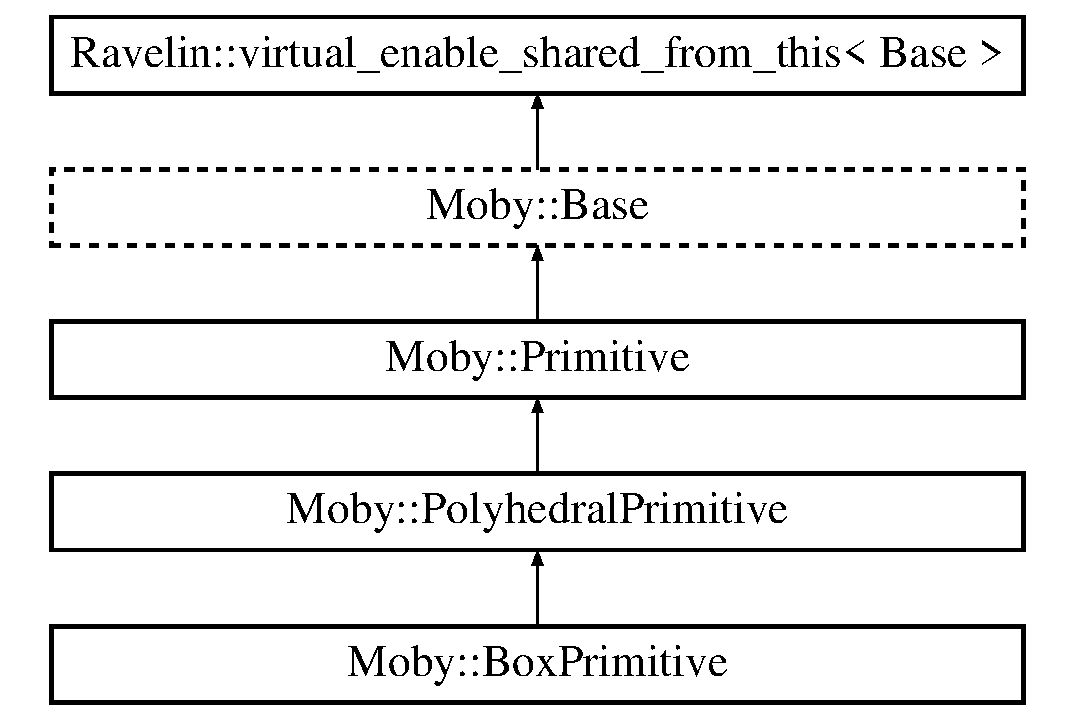
\includegraphics[height=5.000000cm]{classMoby_1_1BoxPrimitive}
\end{center}
\end{figure}
\subsection*{Public Member Functions}
\begin{DoxyCompactItemize}
\item 
{\bf Box\-Primitive} ()\label{classMoby_1_1BoxPrimitive_a9714cb80a5753b347ffffc6ea443017e}

\begin{DoxyCompactList}\small\item\em Constructs a unit cube centered at the origin. \end{DoxyCompactList}\item 
{\bf Box\-Primitive} (double xlen, double ylen, double zlen)\label{classMoby_1_1BoxPrimitive_a9c2e101fcc2b4f032d31c046b49a215d}

\begin{DoxyCompactList}\small\item\em Constructs a box of the specified size. \end{DoxyCompactList}\item 
{\bfseries Box\-Primitive} (double xlen, double ylen, double zlen, const Ravelin\-::\-Pose3d \&T)\label{classMoby_1_1BoxPrimitive_a7346d95be6016eb7b29fcf09ac9697f7}

\item 
{\bfseries Box\-Primitive} (const Ravelin\-::\-Pose3d \&T)\label{classMoby_1_1BoxPrimitive_ac41458ab7e48e5b6ac4c427e50965bf0}

\item 
virtual void {\bf set\-\_\-polyhedron} (const {\bf Polyhedron} \&p)\label{classMoby_1_1BoxPrimitive_a6a4bb0ee868ece8fdf982e7058de6714}

\begin{DoxyCompactList}\small\item\em Overrides the Polyhedron\-Primitive\-::set\-\_\-polyhedron(.) \end{DoxyCompactList}\item 
void {\bf set\-\_\-size} (double xlen, double ylen, double zlen)
\begin{DoxyCompactList}\small\item\em Sets the size of this box. \end{DoxyCompactList}\item 
virtual unsigned {\bfseries num\-\_\-facets} () const \label{classMoby_1_1BoxPrimitive_ab934592fc7a178c08bb4770e63bd9870}

\item 
virtual bool {\bf is\-\_\-convex} () const \label{classMoby_1_1BoxPrimitive_a3e34153ce5004f80174f77558dffeca1}

\begin{DoxyCompactList}\small\item\em Determines whether the primitive is convex. \end{DoxyCompactList}\item 
virtual void {\bf load\-\_\-from\-\_\-xml} (boost\-::shared\-\_\-ptr$<$ const {\bf X\-M\-L\-Tree} $>$ node, std\-::map$<$ std\-::string, {\bf Base\-Ptr} $>$ \&id\-\_\-map)\label{classMoby_1_1BoxPrimitive_a3d40e1f701caccca8fbdf8cbc473b788}

\begin{DoxyCompactList}\small\item\em Implements \doxyref{Base\-::load\-\_\-from\-\_\-xml()}{p.}{classMoby_1_1Base_a98b861c1d615a748b576aa613f17389f} for serialization. \end{DoxyCompactList}\item 
virtual void {\bf save\-\_\-to\-\_\-xml} ({\bf X\-M\-L\-Tree\-Ptr} node, std\-::list$<$ boost\-::shared\-\_\-ptr$<$ const {\bf Base} $>$ $>$ \&shared\-\_\-objects) const \label{classMoby_1_1BoxPrimitive_a7567d7f558da7d8ee30993edb465e8ab}

\begin{DoxyCompactList}\small\item\em Implements \doxyref{Base\-::save\-\_\-to\-\_\-xml()}{p.}{classMoby_1_1Base_aed64905ca39893d02d1e6c3f03f73aa9} for serialization. \end{DoxyCompactList}\item 
virtual {\bf B\-V\-Ptr} {\bf get\-\_\-\-B\-V\-H\-\_\-root} ({\bf Collision\-Geometry\-Ptr} geom)\label{classMoby_1_1BoxPrimitive_a41d65701bf4ba6cf69301eb2bf102f97}

\begin{DoxyCompactList}\small\item\em Gets the bounding volume for this plane. \end{DoxyCompactList}\item 
virtual double {\bf calc\-\_\-dist\-\_\-and\-\_\-normal} (const {\bf Point3d} \&point, std\-::vector$<$ Ravelin\-::\-Vector3d $>$ \&normals) const \label{classMoby_1_1BoxPrimitive_a4db9695a126612c821bc962db8d679a3}

\begin{DoxyCompactList}\small\item\em Tests whether a point is inside or on the box. \end{DoxyCompactList}\item 
double {\bf calc\-\_\-closest\-\_\-point} (const {\bf Point3d} \&point, {\bf Point3d} \&closest) const \label{classMoby_1_1BoxPrimitive_ad1b96f3b923526fb535809838eb0eee2}

\begin{DoxyCompactList}\small\item\em Computes the closest point on the box to a point (and returns the distance) \end{DoxyCompactList}\item 
virtual void {\bf set\-\_\-pose} (const Ravelin\-::\-Pose3d \&T)\label{classMoby_1_1BoxPrimitive_a765e606e00ee883c4f0cf86a2b17b503}

\begin{DoxyCompactList}\small\item\em Transforms the primitive. \end{DoxyCompactList}\item 
void {\bf set\-\_\-edge\-\_\-sample\-\_\-length} (double len)\label{classMoby_1_1BoxPrimitive_ac9ff590377ec5716ae8a78db9758bf41}

\begin{DoxyCompactList}\small\item\em Sets the edge sample length for this box. \end{DoxyCompactList}\item 
virtual boost\-::shared\-\_\-ptr\\*
$<$ const {\bf Indexed\-Tri\-Array} $>$ {\bf get\-\_\-mesh} (boost\-::shared\-\_\-ptr$<$ const Ravelin\-::\-Pose3d $>$ P)
\begin{DoxyCompactList}\small\item\em Gets the set of vertices for the \doxyref{Box\-Primitive}{p.}{classMoby_1_1BoxPrimitive} (constructing, if necessary) \end{DoxyCompactList}\item 
virtual osg\-::\-Node $\ast$ {\bf create\-\_\-visualization} ()\label{classMoby_1_1BoxPrimitive_a48e4775b9cba8ea3086eaff6a7cac809}

\begin{DoxyCompactList}\small\item\em Creates the visualization for this primitive. \end{DoxyCompactList}\item 
double {\bfseries calc\-\_\-signed\-\_\-dist} (boost\-::shared\-\_\-ptr$<$ const {\bf Sphere\-Primitive} $>$ s, {\bf Point3d} \&pthis, {\bf Point3d} \&psph) const \label{classMoby_1_1BoxPrimitive_a71fd11eedd20ba5cf5f971623cd905ff}

\item 
virtual double {\bf calc\-\_\-signed\-\_\-dist} (boost\-::shared\-\_\-ptr$<$ const {\bf Primitive} $>$ p, {\bf Point3d} \&pthis, {\bf Point3d} \&pp) const \label{classMoby_1_1BoxPrimitive_afa94e6d28303bab94a3ffdab87d7d3df}

\begin{DoxyCompactList}\small\item\em Computes the signed distance between this and another primitive. \end{DoxyCompactList}\item 
virtual void {\bf get\-\_\-vertices} (boost\-::shared\-\_\-ptr$<$ const Ravelin\-::\-Pose3d $>$ P, std\-::vector$<$ {\bf Point3d} $>$ \&p) const \label{classMoby_1_1BoxPrimitive_a329b84ac213b791173b787fb54996e6c}

\begin{DoxyCompactList}\small\item\em Gets the set of vertices for the \doxyref{Box\-Primitive}{p.}{classMoby_1_1BoxPrimitive}. \end{DoxyCompactList}\item 
virtual double {\bf calc\-\_\-signed\-\_\-dist} (const {\bf Point3d} \&p) const \label{classMoby_1_1BoxPrimitive_a3a8f66228befd2dad762bde3ff3b9b41}

\begin{DoxyCompactList}\small\item\em Computes the signed distance to a point. \end{DoxyCompactList}\item 
double {\bf calc\-\_\-closest\-\_\-points} (boost\-::shared\-\_\-ptr$<$ const {\bf Sphere\-Primitive} $>$ s, {\bf Point3d} \&pbox, {\bf Point3d} \&psph) const \label{classMoby_1_1BoxPrimitive_a3f009bc061038fa7f1ce4405efc66326}

\begin{DoxyCompactList}\small\item\em Finds closest point between a box and a sphere; returns the closest point on/in the box to the center of the sphere. \end{DoxyCompactList}\item 
virtual double {\bfseries get\-\_\-bounding\-\_\-radius} () const \label{classMoby_1_1BoxPrimitive_a3a0bd74748d6c67662907a05d1e77cdc}

\item 
double {\bf get\-\_\-x\-\_\-len} () const \label{classMoby_1_1BoxPrimitive_aa222b496aa25e46765eb5c76c80cd5d0}

\begin{DoxyCompactList}\small\item\em Get the x-\/length of this box. \end{DoxyCompactList}\item 
double {\bf get\-\_\-y\-\_\-len} () const \label{classMoby_1_1BoxPrimitive_a4da4671d5917529f4b96a685b1ae0f07}

\begin{DoxyCompactList}\small\item\em Get the y-\/length of this box. \end{DoxyCompactList}\item 
double {\bf get\-\_\-z\-\_\-len} () const \label{classMoby_1_1BoxPrimitive_a6d5aa13ecd4d574bc8b23fbb3b295db1}

\begin{DoxyCompactList}\small\item\em Ge the z-\/length of this box. \end{DoxyCompactList}\end{DoxyCompactItemize}
\subsection*{Additional Inherited Members}


\subsection{Detailed Description}
Represents a solid box centered at the origin (by default) 

\subsection{Member Function Documentation}
\index{Moby\-::\-Box\-Primitive@{Moby\-::\-Box\-Primitive}!get\-\_\-mesh@{get\-\_\-mesh}}
\index{get\-\_\-mesh@{get\-\_\-mesh}!Moby::BoxPrimitive@{Moby\-::\-Box\-Primitive}}
\subsubsection[{get\-\_\-mesh}]{\setlength{\rightskip}{0pt plus 5cm}shared\-\_\-ptr$<$ const {\bf Indexed\-Tri\-Array} $>$ Box\-Primitive\-::get\-\_\-mesh (
\begin{DoxyParamCaption}
\item[{boost\-::shared\-\_\-ptr$<$ const Ravelin\-::\-Pose3d $>$}]{P}
\end{DoxyParamCaption}
)\hspace{0.3cm}{\ttfamily [virtual]}}\label{classMoby_1_1BoxPrimitive_a49f0cc86fda96f6b86cab280d82c843d}


Gets the set of vertices for the \doxyref{Box\-Primitive}{p.}{classMoby_1_1BoxPrimitive} (constructing, if necessary) 

Recomputes the triangle mesh for the \doxyref{Box\-Primitive}{p.}{classMoby_1_1BoxPrimitive} 

Reimplemented from {\bf Moby\-::\-Polyhedral\-Primitive} \doxyref{}{p.}{classMoby_1_1PolyhedralPrimitive_a33762e3c23305eb7802287e2c8526b6c}.

\index{Moby\-::\-Box\-Primitive@{Moby\-::\-Box\-Primitive}!set\-\_\-size@{set\-\_\-size}}
\index{set\-\_\-size@{set\-\_\-size}!Moby::BoxPrimitive@{Moby\-::\-Box\-Primitive}}
\subsubsection[{set\-\_\-size}]{\setlength{\rightskip}{0pt plus 5cm}void Box\-Primitive\-::set\-\_\-size (
\begin{DoxyParamCaption}
\item[{double}]{xlen, }
\item[{double}]{ylen, }
\item[{double}]{zlen}
\end{DoxyParamCaption}
)}\label{classMoby_1_1BoxPrimitive_aa3f704d576258ab365eb8b3e39bcb090}


Sets the size of this box. 

\begin{DoxyNote}{Note}
forces recomputation of the mesh 
\end{DoxyNote}


References Moby\-::\-Primitive\-::update\-\_\-visualization().



Referenced by load\-\_\-from\-\_\-xml().



The documentation for this class was generated from the following files\-:\begin{DoxyCompactItemize}
\item 
/home/drum/\-Moby/include/\-Moby/Box\-Primitive.\-h\item 
/home/drum/\-Moby/src/Box\-Primitive.\-cpp\end{DoxyCompactItemize}

\section{Moby\-:\-:B\-V Class Reference}
\label{classMoby_1_1BV}\index{Moby\-::\-B\-V@{Moby\-::\-B\-V}}


An abstract bounding volume.  




{\ttfamily \#include $<$B\-V.\-h$>$}

Inheritance diagram for Moby\-:\-:B\-V\-:\begin{figure}[H]
\begin{center}
\leavevmode
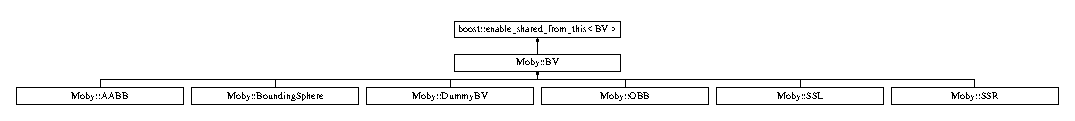
\includegraphics[height=1.171548cm]{classMoby_1_1BV}
\end{center}
\end{figure}
\subsection*{Public Member Functions}
\begin{DoxyCompactItemize}
\item 
virtual std\-::ostream \& {\bf to\-\_\-vrml} (std\-::ostream \&out, const Ravelin\-::\-Pose3d \&T) const =0\label{classMoby_1_1BV_a600fc641a28dba109450ab7b4857cf69}

\begin{DoxyCompactList}\small\item\em Virtual function for outputting the bounding volume to V\-R\-M\-L. \end{DoxyCompactList}\item 
virtual bool {\bf outside} (const {\bf Point3d} \&point, double tol=N\-E\-A\-R\-\_\-\-Z\-E\-R\-O) const =0\label{classMoby_1_1BV_a30fafce97a805a68cc0ff3b3e74a298d}

\begin{DoxyCompactList}\small\item\em Determines whether a point is outside the bounding volume. \end{DoxyCompactList}\item 
virtual bool {\bf intersects} (const {\bf Line\-Seg3} \&seg, double \&tmin, double tmax, {\bf Point3d} \&q) const =0\label{classMoby_1_1BV_a955d2960f336300fcf8512d74975a747}

\begin{DoxyCompactList}\small\item\em Determines whether a line segment intersects the bounding volume. \end{DoxyCompactList}\item 
virtual boost\-::shared\-\_\-ptr\\*
$<$ const Ravelin\-::\-Pose3d $>$ {\bf get\-\_\-relative\-\_\-pose} () const =0\label{classMoby_1_1BV_a89f5b628152241d2c1d2b125e7801a3a}

\begin{DoxyCompactList}\small\item\em Gets the associated pose for this bounding volume. \end{DoxyCompactList}\item 
virtual void {\bf transform} (const Ravelin\-::\-Transform3d \&T, {\bf B\-V} $\ast$result) const =0\label{classMoby_1_1BV_ad26e960f270cad01ab1e28c0129fa32c}

\begin{DoxyCompactList}\small\item\em Virtual function for transforming the \doxyref{B\-V}{p.}{classMoby_1_1BV}. \end{DoxyCompactList}\item 
virtual {\bf B\-V\-Ptr} {\bf calc\-\_\-swept\-\_\-\-B\-V} ({\bf Collision\-Geometry\-Ptr} g, const Ravelin\-::\-S\-Velocityd \&v) const =0
\begin{DoxyCompactList}\small\item\em Virtual function that calculates a velocity-\/expanded \doxyref{B\-V}{p.}{classMoby_1_1BV}. \end{DoxyCompactList}\item 
{\bf B\-V\-Ptr} {\bfseries get\-\_\-this} ()\label{classMoby_1_1BV_a54a5142d6c3b7e7400b52ea93f8a0eb2}

\item 
boost\-::shared\-\_\-ptr$<$ const {\bf B\-V} $>$ {\bfseries get\-\_\-this} () const \label{classMoby_1_1BV_aebe21d442b8d3fb0426b94005ab7a7c2}

\item 
bool {\bfseries is\-\_\-leaf} () const \label{classMoby_1_1BV_a8ffc25a32a69fe64980d51fd182599ea}

\item 
{\footnotesize template$<$class Output\-Iterator $>$ }\\Output\-Iterator {\bf get\-\_\-all\-\_\-\-B\-Vs} (Output\-Iterator begin) const 
\begin{DoxyCompactList}\small\item\em Gets all \doxyref{B\-V}{p.}{classMoby_1_1BV} nodes. \end{DoxyCompactList}\item 
{\footnotesize template$<$class Output\-Iterator $>$ }\\Output\-Iterator {\bf get\-\_\-all\-\_\-leafs} (Output\-Iterator begin) const \label{classMoby_1_1BV_ac75068beeeab413e60364a08d5d0c4f9}

\begin{DoxyCompactList}\small\item\em Gets all leaf nodes. \end{DoxyCompactList}\item 
virtual double {\bf calc\-\_\-volume} () const =0\label{classMoby_1_1BV_aa6f6a534c466e5304462e3007f9c003a}

\begin{DoxyCompactList}\small\item\em Gets the volume for this bounding volume. \end{DoxyCompactList}\item 
virtual {\bf Point3d} {\bf get\-\_\-lower\-\_\-bounds} () const =0\label{classMoby_1_1BV_a1c09ed69ea23c53ee3e392702dbe624f}

\begin{DoxyCompactList}\small\item\em Gets the lower bound on a \doxyref{A\-A\-B\-B}{p.}{classMoby_1_1AABB} around the bounding volume when a transform of T is applied. \end{DoxyCompactList}\item 
virtual {\bf Point3d} {\bf get\-\_\-upper\-\_\-bounds} () const =0\label{classMoby_1_1BV_a49b6075d167dfc05293cb87e28a570ea}

\begin{DoxyCompactList}\small\item\em Gets the upper bound on a \doxyref{A\-A\-B\-B}{p.}{classMoby_1_1AABB} around the bounding volume when a transform of T is applied. \end{DoxyCompactList}\item 
{\footnotesize template$<$class Output\-Iterator $>$ }\\Output\-Iterator {\bf get\-\_\-all\-\_\-\-B\-Vs} (Output\-Iterator begin) const 
\begin{DoxyCompactList}\small\item\em Gets all \doxyref{B\-V}{p.}{classMoby_1_1BV} nodes. \end{DoxyCompactList}\item 
{\footnotesize template$<$class Output\-Iterator $>$ }\\Output\-Iterator {\bf get\-\_\-all\-\_\-leafs} (Output\-Iterator begin) const \label{classMoby_1_1BV_ac75068beeeab413e60364a08d5d0c4f9}

\begin{DoxyCompactList}\small\item\em Gets all leaf nodes. \end{DoxyCompactList}\item 
{\footnotesize template$<$class Output\-Iterator $>$ }\\Output\-Iterator {\bf intersect\-\_\-\-B\-V\-\_\-trees} ({\bf B\-V\-Ptr} a, {\bf B\-V\-Ptr} b, const Ravelin\-::\-Transform3d \&a\-Tb, const Ravelin\-::\-Transform3d \&b\-Ta, Output\-Iterator output\-\_\-begin)
\begin{DoxyCompactList}\small\item\em Intersects two \doxyref{B\-V}{p.}{classMoby_1_1BV} trees; returns list of all leaf-\/level intersecting B\-Vs. \end{DoxyCompactList}\end{DoxyCompactItemize}
\subsection*{Static Public Member Functions}
\begin{DoxyCompactItemize}
\item 
static bool {\bf intersects} ({\bf B\-V\-Ptr} a, {\bf B\-V\-Ptr} b)\label{classMoby_1_1BV_a466876c83c54f406dad65117081405aa}

\begin{DoxyCompactList}\small\item\em Convenience method. \end{DoxyCompactList}\item 
static bool {\bf intersects} ({\bf B\-V\-Ptr} a, {\bf B\-V\-Ptr} b, const Ravelin\-::\-Transform3d \&T)\label{classMoby_1_1BV_ab40bccc22188be183e82b3d73b4c51d4}

\begin{DoxyCompactList}\small\item\em Convenience method. \end{DoxyCompactList}\item 
static double {\bf calc\-\_\-distance} ({\bf B\-V\-Ptr} a, {\bf B\-V\-Ptr} b, {\bf Point3d} \&cp1, {\bf Point3d} \&cp2)\label{classMoby_1_1BV_ab0d895ad9899f2ee2534645013334f33}

\begin{DoxyCompactList}\small\item\em Convenience method. \end{DoxyCompactList}\item 
static double {\bf calc\-\_\-distance} ({\bf B\-V\-Ptr} a, {\bf B\-V\-Ptr} b, const Ravelin\-::\-Transform3d \&a\-Tb, {\bf Point3d} \&cp1, {\bf Point3d} \&cp2)\label{classMoby_1_1BV_adf18114469b3967e7eb474d8f69b9c6f}

\begin{DoxyCompactList}\small\item\em Convenience method. \end{DoxyCompactList}\item 
static bool {\bf intersects} (const {\bf B\-V} $\ast$a, const {\bf B\-V} $\ast$b)\label{classMoby_1_1BV_a17e02ce9372e48914f6cdf588c61374f}

\begin{DoxyCompactList}\small\item\em Computes whether two abstract bounding volumes intersect. \end{DoxyCompactList}\item 
static bool {\bfseries intersects} (const {\bf B\-V} $\ast$a, const {\bf B\-V} $\ast$b, const Ravelin\-::\-Transform3d \&T)\label{classMoby_1_1BV_aed30869b2d65c36a96d0f1d579518dc1}

\item 
static double {\bf calc\-\_\-distance} (const {\bf B\-V} $\ast$a, const {\bf B\-V} $\ast$b, {\bf Point3d} \&cp1, {\bf Point3d} \&cp2)
\begin{DoxyCompactList}\small\item\em Computes the distance between two abstract bounding volumes and stores the closest points. \end{DoxyCompactList}\item 
static double {\bfseries calc\-\_\-distance} (const {\bf B\-V} $\ast$a, const {\bf B\-V} $\ast$b, const Ravelin\-::\-Transform3d \&a\-Tb, {\bf Point3d} \&cp1, {\bf Point3d} \&cp2)\label{classMoby_1_1BV_ac138dd07768d3ea36724a0b409346081}

\item 
{\footnotesize template$<$class Output\-Iterator $>$ }\\static Output\-Iterator {\bf intersect\-\_\-\-B\-V\-\_\-trees} ({\bf B\-V\-Ptr} a, {\bf B\-V\-Ptr} b, const Ravelin\-::\-Transform3d \&a\-Tb, const Ravelin\-::\-Transform3d \&b\-Ta, Output\-Iterator output\-\_\-begin)
\begin{DoxyCompactList}\small\item\em Intersects two \doxyref{B\-V}{p.}{classMoby_1_1BV} trees; returns list of all leaf-\/level intersecting B\-Vs. \end{DoxyCompactList}\end{DoxyCompactItemize}
\subsection*{Public Attributes}
\begin{DoxyCompactItemize}
\item 
boost\-::shared\-\_\-ptr$<$ void $>$ {\bf userdata}\label{classMoby_1_1BV_a5fbb63e2c0fb94f2a7f9e25e237d91e9}

\begin{DoxyCompactList}\small\item\em Userdata for the \doxyref{B\-V}{p.}{classMoby_1_1BV}. \end{DoxyCompactList}\item 
{\bf Collision\-Geometry\-Ptr} {\bf geom}\label{classMoby_1_1BV_ad9f99181ae98414e43a0696ae82f33a5}

\begin{DoxyCompactList}\small\item\em The collision geometry associated with this bounding volume. \end{DoxyCompactList}\item 
std\-::list$<$ {\bf B\-V\-Ptr} $>$ {\bf children}\label{classMoby_1_1BV_ad0fe49bf0780f27bdd14019721d757c4}

\begin{DoxyCompactList}\small\item\em The children of this \doxyref{B\-V}{p.}{classMoby_1_1BV}. \end{DoxyCompactList}\end{DoxyCompactItemize}


\subsection{Detailed Description}
An abstract bounding volume. 

\begin{DoxyNote}{Note}
the \doxyref{B\-V}{p.}{classMoby_1_1BV} is generally constructed such that its frame is aligned with that of the underlying rigid body (or collision geometry). Therefore, the center of the \doxyref{B\-V}{p.}{classMoby_1_1BV} is computed relative to the center-\/of-\/mass of the body (or the center of the geometry). The orientation of the \doxyref{B\-V}{p.}{classMoby_1_1BV} will always be identical to the orientation of the rigid body (or collision geometry). 
\end{DoxyNote}


\subsection{Member Function Documentation}
\index{Moby\-::\-B\-V@{Moby\-::\-B\-V}!calc\-\_\-distance@{calc\-\_\-distance}}
\index{calc\-\_\-distance@{calc\-\_\-distance}!Moby::BV@{Moby\-::\-B\-V}}
\subsubsection[{calc\-\_\-distance}]{\setlength{\rightskip}{0pt plus 5cm}double B\-V\-::calc\-\_\-distance (
\begin{DoxyParamCaption}
\item[{const {\bf B\-V} $\ast$}]{a, }
\item[{const {\bf B\-V} $\ast$}]{b, }
\item[{{\bf Point3d} \&}]{cp1, }
\item[{{\bf Point3d} \&}]{cp2}
\end{DoxyParamCaption}
)\hspace{0.3cm}{\ttfamily [static]}}\label{classMoby_1_1BV_a989e55f8255842a4bfbd18deb048f886}


Computes the distance between two abstract bounding volumes and stores the closest points. 


\begin{DoxyParams}{Parameters}
{\em cp1} & the closest point on a to b \\
\hline
{\em cp2} & the closest point on b to a \\
\hline
\end{DoxyParams}
\begin{DoxyReturn}{Returns}
the distance between the bounding volumes 
\end{DoxyReturn}
\index{Moby\-::\-B\-V@{Moby\-::\-B\-V}!calc\-\_\-swept\-\_\-\-B\-V@{calc\-\_\-swept\-\_\-\-B\-V}}
\index{calc\-\_\-swept\-\_\-\-B\-V@{calc\-\_\-swept\-\_\-\-B\-V}!Moby::BV@{Moby\-::\-B\-V}}
\subsubsection[{calc\-\_\-swept\-\_\-\-B\-V}]{\setlength{\rightskip}{0pt plus 5cm}virtual {\bf B\-V\-Ptr} Moby\-::\-B\-V\-::calc\-\_\-swept\-\_\-\-B\-V (
\begin{DoxyParamCaption}
\item[{{\bf Collision\-Geometry\-Ptr}}]{g, }
\item[{const Ravelin\-::\-S\-Velocityd \&}]{v}
\end{DoxyParamCaption}
) const\hspace{0.3cm}{\ttfamily [pure virtual]}}\label{classMoby_1_1BV_a6aeddf29519a8d71d7318ca406d84582}


Virtual function that calculates a velocity-\/expanded \doxyref{B\-V}{p.}{classMoby_1_1BV}. 


\begin{DoxyParams}{Parameters}
{\em g} & the geometry that this bounding volume represents \\
\hline
{\em v} & the \char`\"{}velocity\char`\"{} to sweep by \\
\hline
\end{DoxyParams}
\begin{DoxyReturn}{Returns}
the velocity-\/expanded bounding volume 
\end{DoxyReturn}


Implemented in {\bf Moby\-::\-Dummy\-B\-V} \doxyref{}{p.}{classMoby_1_1DummyBV_a025ef57dac043eb93f23f250e3817b7a}, {\bf Moby\-::\-O\-B\-B} \doxyref{}{p.}{classMoby_1_1OBB_af319672a637c35433069cc1d84c1288c}, {\bf Moby\-::\-S\-S\-R} \doxyref{}{p.}{classMoby_1_1SSR_a455c8f91015dc88fd82e401d29cc3b04}, {\bf Moby\-::\-S\-S\-L} \doxyref{}{p.}{classMoby_1_1SSL_a6984388248b9437ce29433de1a264234}, {\bf Moby\-::\-A\-A\-B\-B} \doxyref{}{p.}{classMoby_1_1AABB_a975b51863c80296821a52884f8d40e85}, and {\bf Moby\-::\-Bounding\-Sphere} \doxyref{}{p.}{classMoby_1_1BoundingSphere_a6d265cdebfde00b3590984c378a238ea}.

\index{Moby\-::\-B\-V@{Moby\-::\-B\-V}!get\-\_\-all\-\_\-\-B\-Vs@{get\-\_\-all\-\_\-\-B\-Vs}}
\index{get\-\_\-all\-\_\-\-B\-Vs@{get\-\_\-all\-\_\-\-B\-Vs}!Moby::BV@{Moby\-::\-B\-V}}
\subsubsection[{get\-\_\-all\-\_\-\-B\-Vs}]{\setlength{\rightskip}{0pt plus 5cm}template$<$class Output\-Iterator $>$ Output\-Iterator Moby\-::\-B\-V\-::get\-\_\-all\-\_\-\-B\-Vs (
\begin{DoxyParamCaption}
\item[{Output\-Iterator}]{begin}
\end{DoxyParamCaption}
) const}\label{classMoby_1_1BV_a2c413068b22f160e3b4fe08f40bc1359}


Gets all \doxyref{B\-V}{p.}{classMoby_1_1BV} nodes. 

The output is ordered by levels in the hierarchy. \index{Moby\-::\-B\-V@{Moby\-::\-B\-V}!get\-\_\-all\-\_\-\-B\-Vs@{get\-\_\-all\-\_\-\-B\-Vs}}
\index{get\-\_\-all\-\_\-\-B\-Vs@{get\-\_\-all\-\_\-\-B\-Vs}!Moby::BV@{Moby\-::\-B\-V}}
\subsubsection[{get\-\_\-all\-\_\-\-B\-Vs}]{\setlength{\rightskip}{0pt plus 5cm}template$<$class Output\-Iterator $>$ Output\-Iterator Moby\-::\-B\-V\-::get\-\_\-all\-\_\-\-B\-Vs (
\begin{DoxyParamCaption}
\item[{Output\-Iterator}]{begin}
\end{DoxyParamCaption}
) const}\label{classMoby_1_1BV_a2c413068b22f160e3b4fe08f40bc1359}


Gets all \doxyref{B\-V}{p.}{classMoby_1_1BV} nodes. 

The output is ordered by levels in the hierarchy. \index{Moby\-::\-B\-V@{Moby\-::\-B\-V}!intersect\-\_\-\-B\-V\-\_\-trees@{intersect\-\_\-\-B\-V\-\_\-trees}}
\index{intersect\-\_\-\-B\-V\-\_\-trees@{intersect\-\_\-\-B\-V\-\_\-trees}!Moby::BV@{Moby\-::\-B\-V}}
\subsubsection[{intersect\-\_\-\-B\-V\-\_\-trees}]{\setlength{\rightskip}{0pt plus 5cm}template$<$class Output\-Iterator $>$ Output\-Iterator Moby\-::\-B\-V\-::intersect\-\_\-\-B\-V\-\_\-trees (
\begin{DoxyParamCaption}
\item[{{\bf B\-V\-Ptr}}]{a, }
\item[{{\bf B\-V\-Ptr}}]{b, }
\item[{const Ravelin\-::\-Transform3d \&}]{a\-Tb, }
\item[{const Ravelin\-::\-Transform3d \&}]{b\-Ta, }
\item[{Output\-Iterator}]{output\-\_\-begin}
\end{DoxyParamCaption}
)}\label{classMoby_1_1BV_a2c3fe709178d1559b46cc91f25cb8e8a}


Intersects two \doxyref{B\-V}{p.}{classMoby_1_1BV} trees; returns list of all leaf-\/level intersecting B\-Vs. 


\begin{DoxyParams}{Parameters}
{\em a} & the root of the first \doxyref{B\-V}{p.}{classMoby_1_1BV} tree \\
\hline
{\em b} & the root of the second \doxyref{B\-V}{p.}{classMoby_1_1BV} tree \\
\hline
{\em a\-Tb} & the transform from b's frame to a's frame (i.\-e., inverse(transform(a)) $\ast$ transform(b)) \\
\hline
{\em b\-Ta} & the transform from a's frame to b's frame (i.\-e., inverse(transform(b)) $\ast$ transform(a)) \\
\hline
{\em output\-\_\-begin} & iterator to the beginning of a list of pairs of type pair$<$shared\-\_\-ptr$<$\-B\-V$>$, shared\-\_\-ptr$<$\-B\-V$>$ $>$; first element in each pair comes from the first \doxyref{B\-V}{p.}{classMoby_1_1BV} tree, second element comes from the second tree \\
\hline
\end{DoxyParams}
\begin{DoxyReturn}{Returns}
iterator to the end of a list of pairs of type pair$<$shared\-\_\-ptr$<$\-B\-V$>$, shared\-\_\-ptr$<$\-B\-V$>$ $>$; first element in each pair comes from the first \doxyref{B\-V}{p.}{classMoby_1_1BV} tree, second element comes from the second tree 
\end{DoxyReturn}
\index{Moby\-::\-B\-V@{Moby\-::\-B\-V}!intersect\-\_\-\-B\-V\-\_\-trees@{intersect\-\_\-\-B\-V\-\_\-trees}}
\index{intersect\-\_\-\-B\-V\-\_\-trees@{intersect\-\_\-\-B\-V\-\_\-trees}!Moby::BV@{Moby\-::\-B\-V}}
\subsubsection[{intersect\-\_\-\-B\-V\-\_\-trees}]{\setlength{\rightskip}{0pt plus 5cm}template$<$class Output\-Iterator $>$ Output\-Iterator Moby\-::\-B\-V\-::intersect\-\_\-\-B\-V\-\_\-trees (
\begin{DoxyParamCaption}
\item[{{\bf B\-V\-Ptr}}]{a, }
\item[{{\bf B\-V\-Ptr}}]{b, }
\item[{const Ravelin\-::\-Transform3d \&}]{a\-Tb, }
\item[{const Ravelin\-::\-Transform3d \&}]{b\-Ta, }
\item[{Output\-Iterator}]{output\-\_\-begin}
\end{DoxyParamCaption}
)\hspace{0.3cm}{\ttfamily [static]}}\label{classMoby_1_1BV_a2c3fe709178d1559b46cc91f25cb8e8a}


Intersects two \doxyref{B\-V}{p.}{classMoby_1_1BV} trees; returns list of all leaf-\/level intersecting B\-Vs. 


\begin{DoxyParams}{Parameters}
{\em a} & the root of the first \doxyref{B\-V}{p.}{classMoby_1_1BV} tree \\
\hline
{\em b} & the root of the second \doxyref{B\-V}{p.}{classMoby_1_1BV} tree \\
\hline
{\em a\-Tb} & the transform from b's frame to a's frame (i.\-e., inverse(transform(a)) $\ast$ transform(b)) \\
\hline
{\em b\-Ta} & the transform from a's frame to b's frame (i.\-e., inverse(transform(b)) $\ast$ transform(a)) \\
\hline
{\em output\-\_\-begin} & iterator to the beginning of a list of pairs of type pair$<$shared\-\_\-ptr$<$\-B\-V$>$, shared\-\_\-ptr$<$\-B\-V$>$ $>$; first element in each pair comes from the first \doxyref{B\-V}{p.}{classMoby_1_1BV} tree, second element comes from the second tree \\
\hline
\end{DoxyParams}
\begin{DoxyReturn}{Returns}
iterator to the end of a list of pairs of type pair$<$shared\-\_\-ptr$<$\-B\-V$>$, shared\-\_\-ptr$<$\-B\-V$>$ $>$; first element in each pair comes from the first \doxyref{B\-V}{p.}{classMoby_1_1BV} tree, second element comes from the second tree 
\end{DoxyReturn}


The documentation for this class was generated from the following files\-:\begin{DoxyCompactItemize}
\item 
/home/drum/\-Moby/include/\-Moby/B\-V.\-h\item 
/home/drum/\-Moby/include/\-Moby/B\-V.\-inl\item 
/home/drum/\-Moby/src/B\-V.\-cpp\end{DoxyCompactItemize}

\section{Moby\-:\-:C\-C\-D Class Reference}
\label{classMoby_1_1CCD}\index{Moby\-::\-C\-C\-D@{Moby\-::\-C\-C\-D}}


Implements the \doxyref{Collision\-Detection}{p.}{classMoby_1_1CollisionDetection} abstract class to perform exact contact finding using abstract shapes.  




{\ttfamily \#include $<$C\-C\-D.\-h$>$}

Inheritance diagram for Moby\-:\-:C\-C\-D\-:\begin{figure}[H]
\begin{center}
\leavevmode
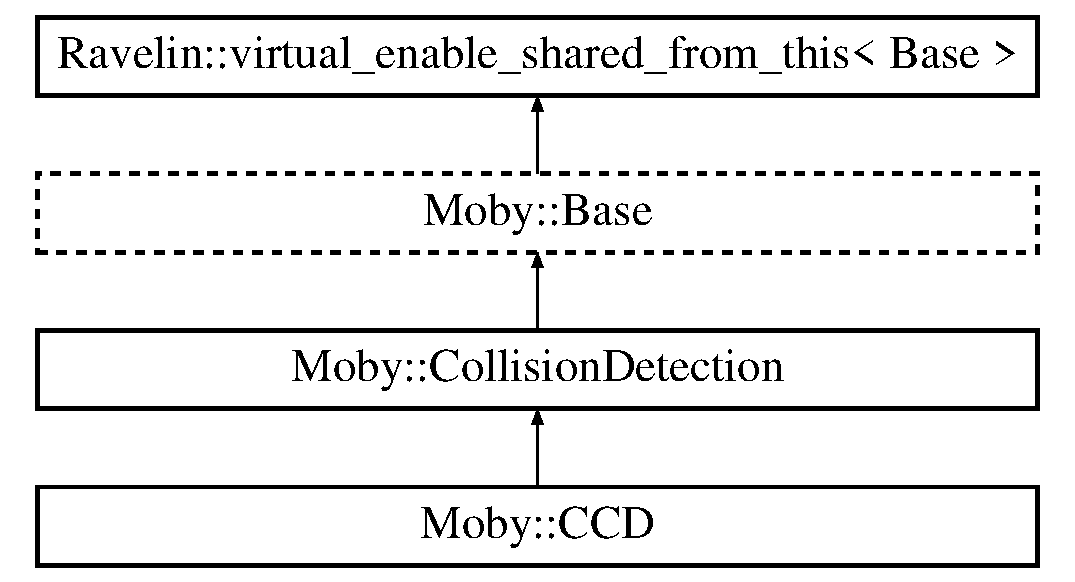
\includegraphics[height=4.000000cm]{classMoby_1_1CCD}
\end{center}
\end{figure}
\subsection*{Public Member Functions}
\begin{DoxyCompactItemize}
\item 
{\bf C\-C\-D} ()\label{classMoby_1_1CCD_a429242f48ff0e1ac536e0849644c1859}

\begin{DoxyCompactList}\small\item\em Constructs a collision detector with default tolerances. \end{DoxyCompactList}\item 
virtual void {\bf load\-\_\-from\-\_\-xml} (boost\-::shared\-\_\-ptr$<$ const {\bf X\-M\-L\-Tree} $>$ node, std\-::map$<$ std\-::string, {\bf Base\-Ptr} $>$ \&id\-\_\-map)\label{classMoby_1_1CCD_ac2537ed877fb1303bcef42fe372e61d5}

\begin{DoxyCompactList}\small\item\em Implements \doxyref{Base\-::load\-\_\-from\-\_\-xml()}{p.}{classMoby_1_1Base_a98b861c1d615a748b576aa613f17389f} \end{DoxyCompactList}\item 
virtual void {\bf save\-\_\-to\-\_\-xml} ({\bf X\-M\-L\-Tree\-Ptr} node, std\-::list$<$ boost\-::shared\-\_\-ptr$<$ const {\bf Base} $>$ $>$ \&shared\-\_\-objects) const 
\begin{DoxyCompactList}\small\item\em Implements \doxyref{Base\-::save\-\_\-to\-\_\-xml()}{p.}{classMoby_1_1Base_aed64905ca39893d02d1e6c3f03f73aa9} \end{DoxyCompactList}\item 
virtual void {\bf broad\-\_\-phase} (double dt, const std\-::vector$<$ {\bf Controlled\-Body\-Ptr} $>$ \&bodies, std\-::vector$<$ std\-::pair$<$ {\bf Collision\-Geometry\-Ptr}, {\bf Collision\-Geometry\-Ptr} $>$ $>$ \&to\-\_\-check)\label{classMoby_1_1CCD_ab7c50d0ee1a90ec79dc784ce5c67eda7}

\begin{DoxyCompactList}\small\item\em Default broad phase function (checks everything) \end{DoxyCompactList}\item 
virtual double {\bf calc\-\_\-\-C\-A\-\_\-\-Euler\-\_\-step} (const {\bf Pairwise\-Dist\-Info} \&pdi)\label{classMoby_1_1CCD_ae6d895289be3908e7d693ccb98d33219}

\begin{DoxyCompactList}\small\item\em Computes a conservative advancement step between two collision geometries assuming that velocity is constant over the interval. \end{DoxyCompactList}\item 
virtual void {\bfseries find\-\_\-contacts} ({\bf Collision\-Geometry\-Ptr} cg\-A, {\bf Collision\-Geometry\-Ptr} cg\-B, std\-::vector$<$ {\bf Unilateral\-Constraint} $>$ \&contacts, double T\-O\-L=N\-E\-A\-R\-\_\-\-Z\-E\-R\-O)\label{classMoby_1_1CCD_ad519517b741dd43212133a1b5cd72754}

\item 
{\footnotesize template$<$class Output\-Iterator $>$ }\\Output\-Iterator {\bf find\-\_\-contacts} ({\bf Collision\-Geometry\-Ptr} cg\-A, {\bf Collision\-Geometry\-Ptr} cg\-B, Output\-Iterator output\-\_\-begin, double T\-O\-L=N\-E\-A\-R\-\_\-\-Z\-E\-R\-O)\label{classMoby_1_1CCD_a2fd35bb15504156ecc8f68fd4d511787}

\begin{DoxyCompactList}\small\item\em Determines contact data between two geometries that are touching or interpenetrating. \end{DoxyCompactList}\item 
{\footnotesize template$<$class Bidirectional\-Iterator $>$ }\\void {\bf insertion\-\_\-sort} (Bidirectional\-Iterator first, Bidirectional\-Iterator last)\label{classMoby_1_1CCD_af6b80150bc1893d248fc011c21f8ed29}

\begin{DoxyCompactList}\small\item\em Does insertion sort -- custom comparison function not supported (uses operator$<$) \end{DoxyCompactList}\item 
{\footnotesize template$<$class Output\-Iterator $>$ }\\Output\-Iterator {\bf find\-\_\-contacts} ({\bf Collision\-Geometry\-Ptr} cg\-A, {\bf Collision\-Geometry\-Ptr} cg\-B, Output\-Iterator output\-\_\-begin, double T\-O\-L)\label{classMoby_1_1CCD_a033267eec0d1dfcefa85d9b200bc3b3e}

\begin{DoxyCompactList}\small\item\em Determines contact data between two geometries that are touching or interpenetrating. \end{DoxyCompactList}\item 
{\footnotesize template$<$class Output\-Iterator $>$ }\\Output\-Iterator {\bf find\-\_\-contacts\-\_\-polyhedron\-\_\-polyhedron} ({\bf Collision\-Geometry\-Ptr} cg\-A, {\bf Collision\-Geometry\-Ptr} cg\-B, Output\-Iterator output\-\_\-begin, double T\-O\-L)\label{classMoby_1_1CCD_a2a62472c5111f72bad9320d458d95bf7}

\begin{DoxyCompactList}\small\item\em Finds contacts between two polyhedra. \end{DoxyCompactList}\item 
{\footnotesize template$<$class Output\-Iterator $>$ }\\Output\-Iterator {\bfseries find\-\_\-contacts\-\_\-vertex\-\_\-vertex} ({\bf Collision\-Geometry\-Ptr} cg\-A, {\bf Collision\-Geometry\-Ptr} cg\-B, boost\-::shared\-\_\-ptr$<$ {\bf Polyhedron\-::\-Vertex} $>$ v1, boost\-::shared\-\_\-ptr$<$ {\bf Polyhedron\-::\-Vertex} $>$ v2, double signed\-\_\-dist, Output\-Iterator output\-\_\-begin)\label{classMoby_1_1CCD_a96214d40bc14dc8b290fd2cdde6a5375}

\item 
{\footnotesize template$<$class Output\-Iterator $>$ }\\Output\-Iterator {\bfseries find\-\_\-contacts\-\_\-vertex\-\_\-edge} ({\bf Collision\-Geometry\-Ptr} cg\-A, {\bf Collision\-Geometry\-Ptr} cg\-B, boost\-::shared\-\_\-ptr$<$ {\bf Polyhedron\-::\-Vertex} $>$ v, boost\-::shared\-\_\-ptr$<$ {\bf Polyhedron\-::\-Edge} $>$ e, double signed\-\_\-dist, Output\-Iterator output\-\_\-begin)\label{classMoby_1_1CCD_a8cfd38be3b300a5dbb6dde88e3d96b9e}

\item 
{\footnotesize template$<$class Output\-Iterator $>$ }\\Output\-Iterator {\bfseries find\-\_\-contacts\-\_\-vertex\-\_\-face} ({\bf Collision\-Geometry\-Ptr} cg\-A, {\bf Collision\-Geometry\-Ptr} cg\-B, boost\-::shared\-\_\-ptr$<$ {\bf Polyhedron\-::\-Vertex} $>$ v\-A, boost\-::shared\-\_\-ptr$<$ {\bf Polyhedron\-::\-Face} $>$ f\-B, double signed\-\_\-dist, Output\-Iterator output\-\_\-begin)\label{classMoby_1_1CCD_a2655b415f4d5a70f8e6c970a558ae263}

\item 
{\footnotesize template$<$class Output\-Iterator $>$ }\\Output\-Iterator {\bfseries find\-\_\-contacts\-\_\-edge\-\_\-edge} ({\bf Collision\-Geometry\-Ptr} cg\-A, {\bf Collision\-Geometry\-Ptr} cg\-B, boost\-::shared\-\_\-ptr$<$ {\bf Polyhedron\-::\-Edge} $>$ e1, boost\-::shared\-\_\-ptr$<$ {\bf Polyhedron\-::\-Edge} $>$ e2, double signed\-\_\-dist, Output\-Iterator output\-\_\-begin)\label{classMoby_1_1CCD_a323af5cad6abd0ceb11c7a0a06bd8d8f}

\item 
{\footnotesize template$<$class Output\-Iterator $>$ }\\Output\-Iterator {\bfseries find\-\_\-contacts\-\_\-edge\-\_\-face} ({\bf Collision\-Geometry\-Ptr} cg\-A, {\bf Collision\-Geometry\-Ptr} cg\-B, boost\-::shared\-\_\-ptr$<$ {\bf Polyhedron\-::\-Edge} $>$ e\-A, boost\-::shared\-\_\-ptr$<$ {\bf Polyhedron\-::\-Face} $>$ f\-B, double signed\-\_\-dist, Output\-Iterator output\-\_\-begin)\label{classMoby_1_1CCD_aaa067166ed3f0f57762c3390dcbae786}

\item 
{\footnotesize template$<$class Output\-Iterator $>$ }\\Output\-Iterator {\bfseries find\-\_\-contacts\-\_\-face\-\_\-face} ({\bf Collision\-Geometry\-Ptr} cg\-A, {\bf Collision\-Geometry\-Ptr} cg\-B, boost\-::shared\-\_\-ptr$<$ {\bf Polyhedron\-::\-Face} $>$ f\-A, boost\-::shared\-\_\-ptr$<$ {\bf Polyhedron\-::\-Face} $>$ f\-B, double signed\-\_\-dist, Output\-Iterator output\-\_\-begin)\label{classMoby_1_1CCD_ae4f8fb6ad454757738d07bb4345b1322}

\item 
{\footnotesize template$<$class Output\-Iterator $>$ }\\Output\-Iterator {\bfseries find\-\_\-contacts\-\_\-generic} ({\bf Collision\-Geometry\-Ptr} cg\-A, {\bf Collision\-Geometry\-Ptr} cg\-B, Output\-Iterator output\-\_\-begin, double T\-O\-L)\label{classMoby_1_1CCD_a2903fba0f1e7bca7bf7a3a340a2d4d24}

\item 
{\footnotesize template$<$class Output\-Iterator $>$ }\\Output\-Iterator {\bfseries find\-\_\-contacts\-\_\-cylinder\-\_\-plane} ({\bf Collision\-Geometry\-Ptr} cg\-A, {\bf Collision\-Geometry\-Ptr} cg\-B, Output\-Iterator o, double T\-O\-L)\label{classMoby_1_1CCD_a0d365b79286e3409df49ad9d9931fad6}

\item 
{\footnotesize template$<$class Output\-Iterator $>$ }\\Output\-Iterator {\bfseries find\-\_\-contacts\-\_\-sphere\-\_\-plane} ({\bf Collision\-Geometry\-Ptr} cg\-A, {\bf Collision\-Geometry\-Ptr} cg\-B, Output\-Iterator o, double T\-O\-L)\label{classMoby_1_1CCD_ad998ca8e7c93cf85ecec671df564c302}

\item 
{\footnotesize template$<$class Output\-Iterator $>$ }\\Output\-Iterator {\bfseries find\-\_\-contacts\-\_\-plane\-\_\-generic} ({\bf Collision\-Geometry\-Ptr} cg\-A, {\bf Collision\-Geometry\-Ptr} cg\-B, Output\-Iterator o, double T\-O\-L)\label{classMoby_1_1CCD_a3186861d0f855b3869d5d752f4ba67c8}

\item 
{\footnotesize template$<$class Output\-Iterator $>$ }\\Output\-Iterator {\bfseries find\-\_\-contacts\-\_\-heightmap\-\_\-generic} ({\bf Collision\-Geometry\-Ptr} cg\-A, {\bf Collision\-Geometry\-Ptr} cg\-B, Output\-Iterator o, double T\-O\-L)\label{classMoby_1_1CCD_a99f5c718a3331a7fb120ceca53c5146d}

\item 
{\footnotesize template$<$class Output\-Iterator $>$ }\\Output\-Iterator {\bf find\-\_\-contacts\-\_\-sphere\-\_\-heightmap} ({\bf Collision\-Geometry\-Ptr} cg\-A, {\bf Collision\-Geometry\-Ptr} cg\-B, Output\-Iterator output\-\_\-begin, double T\-O\-L)\label{classMoby_1_1CCD_aa44d9b3bcf7435542138334fb79b3211}

\begin{DoxyCompactList}\small\item\em Finds contacts between a sphere and a heightmap. \end{DoxyCompactList}\item 
{\footnotesize template$<$class Output\-Iterator $>$ }\\Output\-Iterator {\bf find\-\_\-contacts\-\_\-convex\-\_\-heightmap} ({\bf Collision\-Geometry\-Ptr} cg\-A, {\bf Collision\-Geometry\-Ptr} cg\-B, Output\-Iterator output\-\_\-begin, double T\-O\-L)\label{classMoby_1_1CCD_a8f31261ca1e9f6d90606101e25e16ae0}

\begin{DoxyCompactList}\small\item\em Finds contacts for a convex shape and a heightmap. \end{DoxyCompactList}\item 
{\footnotesize template$<$class Output\-Iterator $>$ }\\Output\-Iterator {\bf find\-\_\-contacts\-\_\-sphere\-\_\-sphere} ({\bf Collision\-Geometry\-Ptr} cg\-A, {\bf Collision\-Geometry\-Ptr} cg\-B, Output\-Iterator output\-\_\-begin, double T\-O\-L)\label{classMoby_1_1CCD_a1a60a578dc9ccdd077a1f7bc58540f1d}

\begin{DoxyCompactList}\small\item\em Finds contacts for two spheres (one piece of code works for both separated and non-\/separated spheres) \end{DoxyCompactList}\item 
{\footnotesize template$<$class Output\-Iterator $>$ }\\Output\-Iterator {\bf find\-\_\-contacts\-\_\-box\-\_\-sphere} ({\bf Collision\-Geometry\-Ptr} cg\-A, {\bf Collision\-Geometry\-Ptr} cg\-B, Output\-Iterator o, double T\-O\-L)\label{classMoby_1_1CCD_a1df51ebbda44ad9d47da50d90afbd9f2}

\begin{DoxyCompactList}\small\item\em Gets contact points between a box and a sphere. \end{DoxyCompactList}\item 
{\footnotesize template$<$class Output\-Iterator $>$ }\\Output\-Iterator {\bf find\-\_\-contacts\-\_\-torus\-\_\-plane} ({\bf Collision\-Geometry\-Ptr} cg\-A, {\bf Collision\-Geometry\-Ptr} cg\-B, Output\-Iterator o, double T\-O\-L)\label{classMoby_1_1CCD_ad58eca1925cc3a12402cfe92948b0b95}

\begin{DoxyCompactList}\small\item\em Gets contact points between a torus and a plane. \end{DoxyCompactList}\item 
{\footnotesize template$<$class Bidirectional\-Iterator $>$ }\\void {\bf insertion\-\_\-sort} (Bidirectional\-Iterator first, Bidirectional\-Iterator last)\label{classMoby_1_1CCD_af6b80150bc1893d248fc011c21f8ed29}

\begin{DoxyCompactList}\small\item\em Does insertion sort -- custom comparison function not supported (uses operator$<$) \end{DoxyCompactList}\end{DoxyCompactItemize}
\subsection*{Static Public Member Functions}
\begin{DoxyCompactItemize}
\item 
static unsigned {\bfseries constrain\-\_\-unsigned} (int ii, int maxi)\label{classMoby_1_1CCD_a0bd788eb70022b6feb9d15e22cc902ec}

\end{DoxyCompactItemize}
\subsection*{Public Attributes}
\begin{DoxyCompactItemize}
\item 
std\-::set$<$ Ravelin\-::sorted\-\_\-pair\\*
$<$ {\bf Collision\-Geometry\-Ptr} $>$ $>$ {\bf disabled\-\_\-pairs}
\begin{DoxyCompactList}\small\item\em Pairs of collision geometries that aren't checked for contact/collision. \end{DoxyCompactList}\end{DoxyCompactItemize}
\subsection*{Protected Member Functions}
\begin{DoxyCompactItemize}
\item 
virtual double {\bfseries calc\-\_\-next\-\_\-\-C\-A\-\_\-\-Euler\-\_\-step} (const {\bf Pairwise\-Dist\-Info} \&pdi)\label{classMoby_1_1CCD_a0a2c6a28b0321dfae19bdf4db329c5ae}

\end{DoxyCompactItemize}
\subsection*{Additional Inherited Members}


\subsection{Detailed Description}
Implements the \doxyref{Collision\-Detection}{p.}{classMoby_1_1CollisionDetection} abstract class to perform exact contact finding using abstract shapes. 

\subsection{Member Function Documentation}
\index{Moby\-::\-C\-C\-D@{Moby\-::\-C\-C\-D}!save\-\_\-to\-\_\-xml@{save\-\_\-to\-\_\-xml}}
\index{save\-\_\-to\-\_\-xml@{save\-\_\-to\-\_\-xml}!Moby::CCD@{Moby\-::\-C\-C\-D}}
\subsubsection[{save\-\_\-to\-\_\-xml}]{\setlength{\rightskip}{0pt plus 5cm}void C\-C\-D\-::save\-\_\-to\-\_\-xml (
\begin{DoxyParamCaption}
\item[{{\bf X\-M\-L\-Tree\-Ptr}}]{node, }
\item[{std\-::list$<$ boost\-::shared\-\_\-ptr$<$ const {\bf Base} $>$ $>$ \&}]{shared\-\_\-objects}
\end{DoxyParamCaption}
) const\hspace{0.3cm}{\ttfamily [virtual]}}\label{classMoby_1_1CCD_a9c3cf2fc9e7827ba8bcb584cf2dba31b}


Implements \doxyref{Base\-::save\-\_\-to\-\_\-xml()}{p.}{classMoby_1_1Base_aed64905ca39893d02d1e6c3f03f73aa9} 

\begin{DoxyNote}{Note}
neither the contact cache nor the pairs currently in collision are saved 
\end{DoxyNote}


Reimplemented from {\bf Moby\-::\-Base} \doxyref{}{p.}{classMoby_1_1Base_aed64905ca39893d02d1e6c3f03f73aa9}.



\subsection{Member Data Documentation}
\index{Moby\-::\-C\-C\-D@{Moby\-::\-C\-C\-D}!disabled\-\_\-pairs@{disabled\-\_\-pairs}}
\index{disabled\-\_\-pairs@{disabled\-\_\-pairs}!Moby::CCD@{Moby\-::\-C\-C\-D}}
\subsubsection[{disabled\-\_\-pairs}]{\setlength{\rightskip}{0pt plus 5cm}std\-::set$<$Ravelin\-::sorted\-\_\-pair$<${\bf Collision\-Geometry\-Ptr}$>$ $>$ Moby\-::\-C\-C\-D\-::disabled\-\_\-pairs}\label{classMoby_1_1CCD_a10741909c60ac53956b459cb124b8fe4}


Pairs of collision geometries that aren't checked for contact/collision. 

\begin{DoxyNote}{Note}
collisions between geometries for two disabled bodies and collisions between geometries for a single body are automatically not checked and do not need to be added to this set. 
\end{DoxyNote}


The documentation for this class was generated from the following files\-:\begin{DoxyCompactItemize}
\item 
/home/drum/\-Moby/include/\-Moby/C\-C\-D.\-h\item 
/home/drum/\-Moby/include/\-Moby/C\-C\-D.\-inl\item 
/home/drum/\-Moby/src/C\-C\-D.\-cpp\end{DoxyCompactItemize}

\section{Moby\-:\-:Ccolor\-Visitor Class Reference}
\label{classMoby_1_1CcolorVisitor}\index{Moby\-::\-Ccolor\-Visitor@{Moby\-::\-Ccolor\-Visitor}}


This O\-S\-G Node\-Visitor colors all Geometry \& Shape\-Drawable of a single node.  




{\ttfamily \#include $<$Color.\-h$>$}

Inheritance diagram for Moby\-:\-:Ccolor\-Visitor\-:\begin{figure}[H]
\begin{center}
\leavevmode
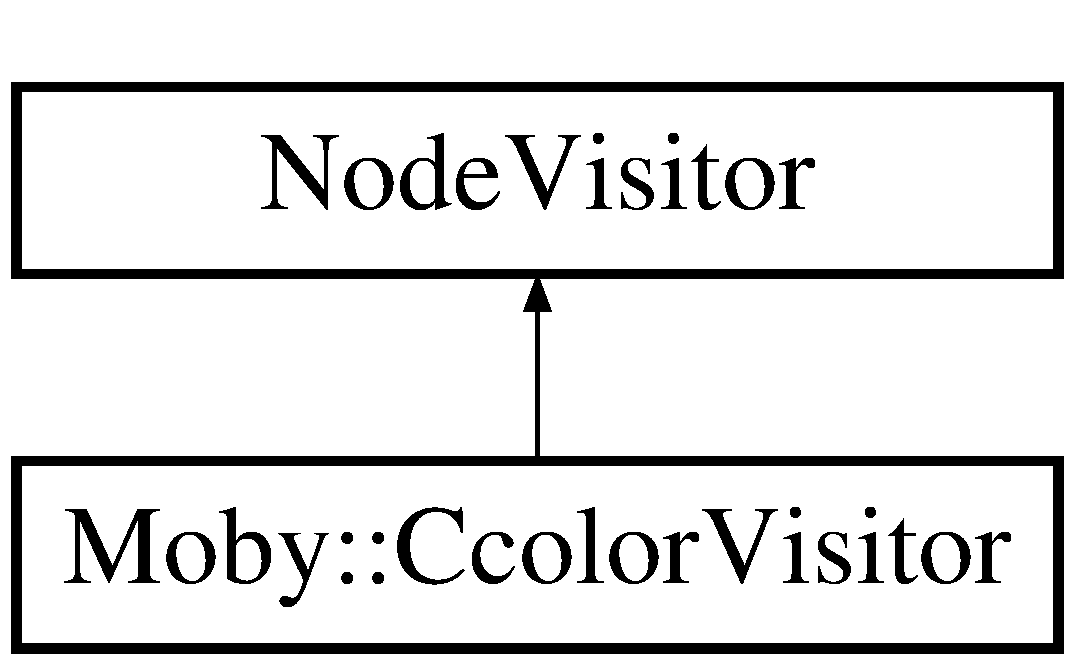
\includegraphics[height=2.000000cm]{classMoby_1_1CcolorVisitor}
\end{center}
\end{figure}
\subsection*{Public Member Functions}
\begin{DoxyCompactItemize}
\item 
{\bfseries Ccolor\-Visitor} (const osg\-::\-Vec4 \&color)\label{classMoby_1_1CcolorVisitor_a32505905c33e1e129e1d02395c5befd3}

\item 
virtual void {\bfseries apply} (osg\-::\-Node \&node)\label{classMoby_1_1CcolorVisitor_a6036f033e8b917cc749737436bbda7c1}

\item 
virtual void {\bfseries apply} (osg\-::\-Geode \&geode)\label{classMoby_1_1CcolorVisitor_a2538ada9c5ab015e8636cc0b4d7fec7e}

\item 
void {\bfseries set\-Color} (const float r, const float g, const float b, const float a=1.\-0f)\label{classMoby_1_1CcolorVisitor_a0af56db971938921aa115a6279a7d337}

\item 
void {\bfseries set\-Color} (const osg\-::\-Vec4 \&color)\label{classMoby_1_1CcolorVisitor_af02ba72ff082fcc06a9fa5644651d444}

\end{DoxyCompactItemize}


\subsection{Detailed Description}
This O\-S\-G Node\-Visitor colors all Geometry \& Shape\-Drawable of a single node. 

usage example\-: \doxyref{Ccolor\-Visitor}{p.}{classMoby_1_1CcolorVisitor} new\-Color; new\-Color.\-set\-Color( r , g , b , a=1.\-0 ); node-\/$>$accept( new\-Color ); 

The documentation for this class was generated from the following file\-:\begin{DoxyCompactItemize}
\item 
/home/drum/\-Moby/src/Color.\-h\end{DoxyCompactItemize}

\section{Moby\-:\-:Collision\-Detection Class Reference}
\label{classMoby_1_1CollisionDetection}\index{Moby\-::\-Collision\-Detection@{Moby\-::\-Collision\-Detection}}


Defines an abstract collision detection mechanism.  




{\ttfamily \#include $<$Collision\-Detection.\-h$>$}

Inheritance diagram for Moby\-:\-:Collision\-Detection\-:\begin{figure}[H]
\begin{center}
\leavevmode
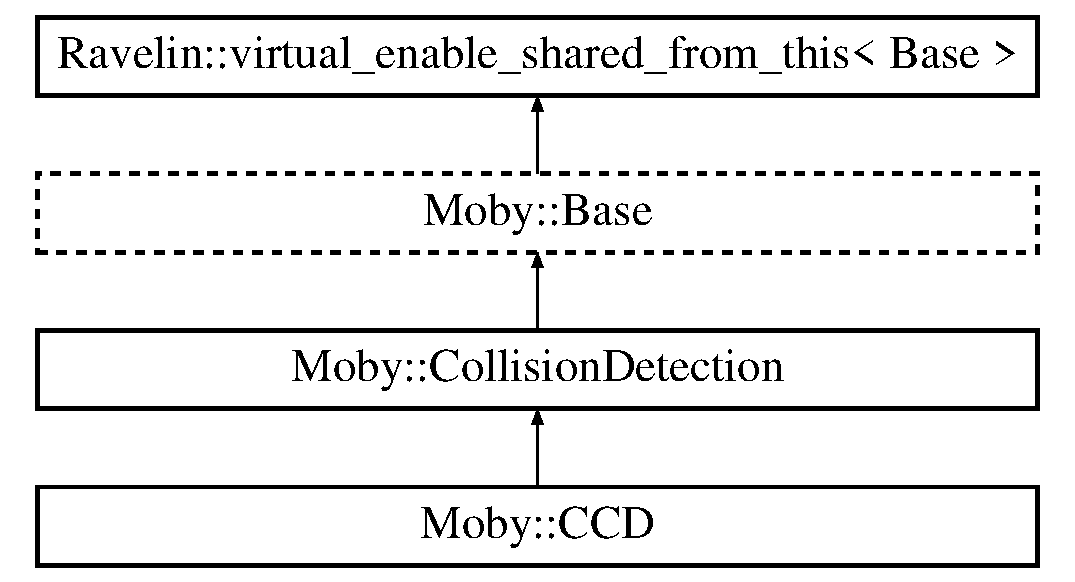
\includegraphics[height=4.000000cm]{classMoby_1_1CollisionDetection}
\end{center}
\end{figure}
\subsection*{Public Member Functions}
\begin{DoxyCompactItemize}
\item 
virtual void {\bfseries set\-\_\-simulator} (boost\-::shared\-\_\-ptr$<$ {\bf Constraint\-Simulator} $>$ sim)\label{classMoby_1_1CollisionDetection_a350e6e1a15595c8bdeda20162e93f076}

\item 
virtual void {\bf broad\-\_\-phase} (double dt, const std\-::vector$<$ {\bf Controlled\-Body\-Ptr} $>$ \&bodies, std\-::vector$<$ std\-::pair$<$ {\bf Collision\-Geometry\-Ptr}, {\bf Collision\-Geometry\-Ptr} $>$ $>$ \&to\-\_\-check)\label{classMoby_1_1CollisionDetection_a2e765b0e2d5b70d6ecf64cb20b2b05d6}

\begin{DoxyCompactList}\small\item\em Default broad phase function (checks everything) \end{DoxyCompactList}\item 
virtual double {\bfseries calc\-\_\-\-C\-A\-\_\-\-Euler\-\_\-step} (const {\bf Pairwise\-Dist\-Info} \&pdi)=0\label{classMoby_1_1CollisionDetection_adb6263442eb74a5351f52a7531b3335a}

\item 
virtual void {\bfseries find\-\_\-contacts} ({\bf Collision\-Geometry\-Ptr} cg\-A, {\bf Collision\-Geometry\-Ptr} cg\-B, std\-::vector$<$ {\bf Unilateral\-Constraint} $>$ \&contacts, double T\-O\-L=N\-E\-A\-R\-\_\-\-Z\-E\-R\-O)=0\label{classMoby_1_1CollisionDetection_a52baefb4b903c5aae59d87830a783533}

\item 
virtual double {\bf calc\-\_\-signed\-\_\-dist} ({\bf Collision\-Geometry\-Ptr} cg1, {\bf Collision\-Geometry\-Ptr} cg2, {\bf Point3d} \&p1, {\bf Point3d} \&p2)\label{classMoby_1_1CollisionDetection_add483854d989e80029d1986bc2976d47}

\begin{DoxyCompactList}\small\item\em Calculates the signed distance between two geometries. \end{DoxyCompactList}\item 
boost\-::shared\-\_\-ptr\\*
$<$ {\bf Collision\-Detection} $>$ {\bf get\-\_\-this} ()\label{classMoby_1_1CollisionDetection_aeaa818a81ebbe2065c8f31731e170bea}

\begin{DoxyCompactList}\small\item\em Get the shared pointer for this. \end{DoxyCompactList}\end{DoxyCompactItemize}
\subsection*{Protected Member Functions}
\begin{DoxyCompactItemize}
\item 
virtual double {\bfseries calc\-\_\-next\-\_\-\-C\-A\-\_\-\-Euler\-\_\-step} (const {\bf Pairwise\-Dist\-Info} \&pdi)=0\label{classMoby_1_1CollisionDetection_a3823cc07abd54647134d108dc9365556}

\end{DoxyCompactItemize}
\subsection*{Static Protected Member Functions}
\begin{DoxyCompactItemize}
\item 
static {\bf Unilateral\-Constraint} {\bf create\-\_\-contact} ({\bf Collision\-Geometry\-Ptr} a, {\bf Collision\-Geometry\-Ptr} b, const {\bf Point3d} \&point, const Ravelin\-::\-Vector3d \&normal, double violation=0.\-0)\label{classMoby_1_1CollisionDetection_ab3f1d864322a2f7f887f372570db672c}

\begin{DoxyCompactList}\small\item\em Creates a contact constraint given the bare-\/minimum info. \end{DoxyCompactList}\end{DoxyCompactItemize}
\subsection*{Friends}
\begin{DoxyCompactItemize}
\item 
class {\bfseries Constraint\-Stabilization}\label{classMoby_1_1CollisionDetection_a320e2b5d0cb83071af150f47d50ca127}

\end{DoxyCompactItemize}
\subsection*{Additional Inherited Members}


\subsection{Detailed Description}
Defines an abstract collision detection mechanism. 

Contact finding and collision detection are two separate, but related, procedures. Collision detection quickly determines whether two bodies are geometrically intersecting at their current configurations. Contact finding determines whether two bodies will come into contact (or are already in contact) in a given time interval; if the bodies do/will contact, contact finding computes contact points and normals. 

The documentation for this class was generated from the following files\-:\begin{DoxyCompactItemize}
\item 
/home/drum/\-Moby/include/\-Moby/Collision\-Detection.\-h\item 
/home/drum/\-Moby/src/Collision\-Detection.\-cpp\end{DoxyCompactItemize}

\section{Moby\-:\-:Collision\-Geometry Class Reference}
\label{classMoby_1_1CollisionGeometry}\index{Moby\-::\-Collision\-Geometry@{Moby\-::\-Collision\-Geometry}}


Defines collision geometry that may be used (in principle) many ways\-: for rigid bodies, non-\/rigid bodies, ...  




{\ttfamily \#include $<$Collision\-Geometry.\-h$>$}

Inheritance diagram for Moby\-:\-:Collision\-Geometry\-:\begin{figure}[H]
\begin{center}
\leavevmode
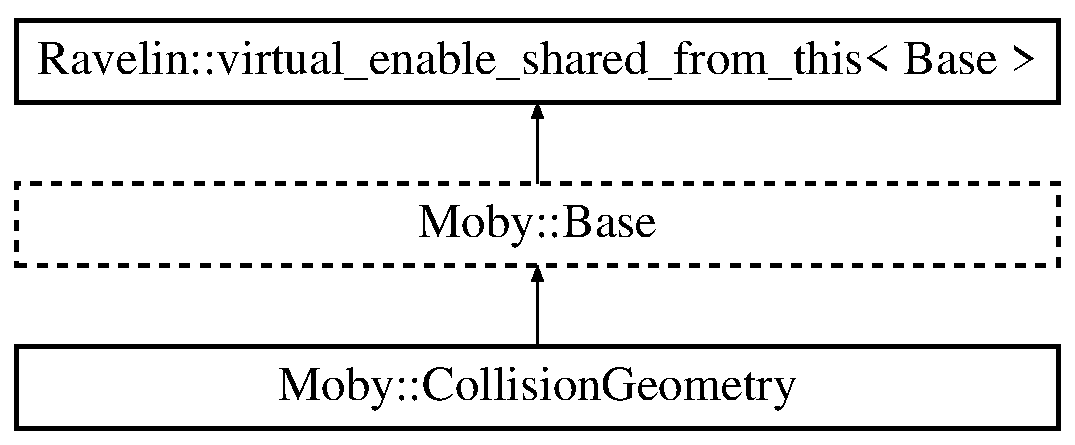
\includegraphics[height=3.000000cm]{classMoby_1_1CollisionGeometry}
\end{center}
\end{figure}
\subsection*{Public Member Functions}
\begin{DoxyCompactItemize}
\item 
{\bf Collision\-Geometry} ()\label{classMoby_1_1CollisionGeometry_a784e93c74cc7d19422511e9d3d6ea863}

\begin{DoxyCompactList}\small\item\em Constructs a \doxyref{Collision\-Geometry}{p.}{classMoby_1_1CollisionGeometry} with no triangle mesh, identity transformation and relative transformation. \end{DoxyCompactList}\item 
void {\bf set\-\_\-relative\-\_\-pose} (const Ravelin\-::\-Pose3d \&pose)
\begin{DoxyCompactList}\small\item\em Sets the relative pose of this geometry. \end{DoxyCompactList}\item 
void {\bf write\-\_\-vrml} (const std\-::string \&filename) const 
\begin{DoxyCompactList}\small\item\em Writes the collision geometry mesh to the specified V\-R\-M\-L file. \end{DoxyCompactList}\item 
{\bf Primitive\-Ptr} {\bf set\-\_\-geometry} ({\bf Primitive\-Ptr} primitive)
\begin{DoxyCompactList}\small\item\em Sets the collision geometry via a primitive. \end{DoxyCompactList}\item 
virtual void {\bf save\-\_\-to\-\_\-xml} ({\bf X\-M\-L\-Tree\-Ptr} node, std\-::list$<$ boost\-::shared\-\_\-ptr$<$ const {\bf Base} $>$ $>$ \&shared\-\_\-objects) const \label{classMoby_1_1CollisionGeometry_a22ac18e99fa56f198d91faecf8b7f8e1}

\begin{DoxyCompactList}\small\item\em Implements \doxyref{Base\-::save\-\_\-to\-\_\-xml()}{p.}{classMoby_1_1Base_aed64905ca39893d02d1e6c3f03f73aa9} \end{DoxyCompactList}\item 
virtual void {\bf load\-\_\-from\-\_\-xml} (boost\-::shared\-\_\-ptr$<$ const {\bf X\-M\-L\-Tree} $>$ node, std\-::map$<$ std\-::string, {\bf Base\-Ptr} $>$ \&id\-\_\-map)\label{classMoby_1_1CollisionGeometry_a164759946c1a08773bc6bea03c3008c8}

\begin{DoxyCompactList}\small\item\em Implements \doxyref{Base\-::load\-\_\-from\-\_\-xml()}{p.}{classMoby_1_1Base_a98b861c1d615a748b576aa613f17389f} \end{DoxyCompactList}\item 
void {\bf set\-\_\-single\-\_\-body} (boost\-::shared\-\_\-ptr$<$ Ravelin\-::\-Single\-Bodyd $>$ s)\label{classMoby_1_1CollisionGeometry_a016bc02ff0f46493b25cd9bee9e9d2df}

\begin{DoxyCompactList}\small\item\em Sets the single body associated with this \doxyref{Collision\-Geometry}{p.}{classMoby_1_1CollisionGeometry}. \end{DoxyCompactList}\item 
double {\bf calc\-\_\-signed\-\_\-dist} (const {\bf Point3d} \&p)\label{classMoby_1_1CollisionGeometry_abb1c300bd5df1aae4eedb61f6960924c}

\begin{DoxyCompactList}\small\item\em Calculates the signed distance for a primitive. \end{DoxyCompactList}\item 
double {\bf calc\-\_\-dist\-\_\-and\-\_\-normal} (const {\bf Point3d} \&p, std\-::vector$<$ Ravelin\-::\-Vector3d $>$ \&n) const \label{classMoby_1_1CollisionGeometry_a705448feff9f2765b2013dae9eb7c8a0}

\begin{DoxyCompactList}\small\item\em Calculates the (unsigned) distance of a point from this collision geometry. \end{DoxyCompactList}\item 
void {\bf get\-\_\-vertices} (std\-::vector$<$ {\bf Point3d} $>$ \&p) const \label{classMoby_1_1CollisionGeometry_ae3aa55120f6c91e387d6423010532b3b}

\begin{DoxyCompactList}\small\item\em Gets vertices for a primitive. \end{DoxyCompactList}\item 
{\bf Point3d} {\bf get\-\_\-supporting\-\_\-point} (const Ravelin\-::\-Vector3d \&d) const \label{classMoby_1_1CollisionGeometry_a287eb3ebf1dbcf95a86b849274303bfd}

\begin{DoxyCompactList}\small\item\em Gets a supporting point for this geometry in a particular direction. \end{DoxyCompactList}\item 
double {\bf get\-\_\-farthest\-\_\-point\-\_\-distance} () const \label{classMoby_1_1CollisionGeometry_af729114ea267bc076c5480359ebc5e34}

\begin{DoxyCompactList}\small\item\em Gets the farthest point from this geometry. \end{DoxyCompactList}\item 
{\bf Collision\-Geometry\-Ptr} {\bf get\-\_\-this} ()\label{classMoby_1_1CollisionGeometry_a06e8a713c28e00acdc66d5b6450b75b2}

\begin{DoxyCompactList}\small\item\em Gets the shared pointer for this. \end{DoxyCompactList}\item 
boost\-::shared\-\_\-ptr\\*
$<$ {\bf Collision\-Geometry} $>$ {\bf get\-\_\-parent} () const \label{classMoby_1_1CollisionGeometry_af83ad26a6662a49a8271356e599cccb7}

\begin{DoxyCompactList}\small\item\em Gets the parent of this \doxyref{Collision\-Geometry}{p.}{classMoby_1_1CollisionGeometry} (or N\-U\-L\-L if there is no parent) \end{DoxyCompactList}\item 
void {\bf set\-\_\-parent} (boost\-::weak\-\_\-ptr$<$ {\bf Collision\-Geometry} $>$ parent)\label{classMoby_1_1CollisionGeometry_a38909e804b12414d12609390407203d9}

\begin{DoxyCompactList}\small\item\em Sets the parent of this \doxyref{Collision\-Geometry}{p.}{classMoby_1_1CollisionGeometry} (or N\-U\-L\-L to indicate no parent) \end{DoxyCompactList}\item 
boost\-::shared\-\_\-ptr$<$ const \\*
Ravelin\-::\-Pose3d $>$ {\bf get\-\_\-pose} () const \label{classMoby_1_1CollisionGeometry_a97fdf323e76b63e0db1b6cbb9e2c7cc4}

\begin{DoxyCompactList}\small\item\em Gets the relative transform for this \doxyref{Collision\-Geometry}{p.}{classMoby_1_1CollisionGeometry}. \end{DoxyCompactList}\item 
boost\-::shared\-\_\-ptr\\*
$<$ Ravelin\-::\-Single\-Bodyd $>$ {\bf get\-\_\-single\-\_\-body} () const \label{classMoby_1_1CollisionGeometry_aafe9c7432f3a629529ebe525b2a3c693}

\begin{DoxyCompactList}\small\item\em Gets the single body associated with this \doxyref{Collision\-Geometry}{p.}{classMoby_1_1CollisionGeometry} (if any) \end{DoxyCompactList}\item 
{\bf Primitive\-Ptr} {\bf get\-\_\-geometry} () const \label{classMoby_1_1CollisionGeometry_afb15f1f785a2286769f6b32eb5b22e74}

\begin{DoxyCompactList}\small\item\em Gets the geometry for this primitive. \end{DoxyCompactList}\end{DoxyCompactItemize}
\subsection*{Static Public Member Functions}
\begin{DoxyCompactItemize}
\item 
static double {\bf calc\-\_\-signed\-\_\-dist} ({\bf Collision\-Geometry\-Ptr} a, {\bf Collision\-Geometry\-Ptr} b, {\bf Point3d} \&cpa, {\bf Point3d} \&cpb)\label{classMoby_1_1CollisionGeometry_ab0db144efbcaa9b47eb68fd7c8c3cbff}

\begin{DoxyCompactList}\small\item\em Calculates the signed distances between two geometries and returns closest points if geometries are not interpenetrating. \end{DoxyCompactList}\end{DoxyCompactItemize}
\subsection*{Public Attributes}
\begin{DoxyCompactItemize}
\item 
double {\bf compliant\-\_\-layer\-\_\-depth}\label{classMoby_1_1CollisionGeometry_a9d26cd90153139bafef2fb0c63337f55}

\begin{DoxyCompactList}\small\item\em The compliant layer around this geometry. \end{DoxyCompactList}\end{DoxyCompactItemize}
\subsection*{Protected Attributes}
\begin{DoxyCompactItemize}
\item 
boost\-::shared\-\_\-ptr\\*
$<$ Ravelin\-::\-Pose3d $>$ {\bf \-\_\-\-F}\label{classMoby_1_1CollisionGeometry_ae72a0959de9c5e3c78c37def1ee89f9e}

\begin{DoxyCompactList}\small\item\em The pose of the \doxyref{Collision\-Geometry}{p.}{classMoby_1_1CollisionGeometry} (relative to the rigid body) \end{DoxyCompactList}\item 
{\bf Primitive\-Ptr} {\bf \-\_\-geometry}\label{classMoby_1_1CollisionGeometry_a6f1e26342336c8a0602a45aedd694f69}

\begin{DoxyCompactList}\small\item\em The underlying geometry. \end{DoxyCompactList}\end{DoxyCompactItemize}
\subsection*{Friends}
\begin{DoxyCompactItemize}
\item 
class {\bfseries Generalized\-C\-C\-D}\label{classMoby_1_1CollisionGeometry_ab5283d85b509bd3e4b0c7187cbb260f5}

\end{DoxyCompactItemize}


\subsection{Detailed Description}
Defines collision geometry that may be used (in principle) many ways\-: for rigid bodies, non-\/rigid bodies, ... 

In principle the geometry may be very complex, and may support nonstationarity (changing over time) or deformities (e.\-g., due to collision). Note that while the underlying geometry may be shared, it is not intended for \doxyref{Collision\-Geometry}{p.}{classMoby_1_1CollisionGeometry} objects to be shared. 

\subsection{Member Function Documentation}
\index{Moby\-::\-Collision\-Geometry@{Moby\-::\-Collision\-Geometry}!set\-\_\-geometry@{set\-\_\-geometry}}
\index{set\-\_\-geometry@{set\-\_\-geometry}!Moby::CollisionGeometry@{Moby\-::\-Collision\-Geometry}}
\subsubsection[{set\-\_\-geometry}]{\setlength{\rightskip}{0pt plus 5cm}{\bf Primitive\-Ptr} Collision\-Geometry\-::set\-\_\-geometry (
\begin{DoxyParamCaption}
\item[{{\bf Primitive\-Ptr}}]{primitive}
\end{DoxyParamCaption}
)}\label{classMoby_1_1CollisionGeometry_a2ac59b456c5ffc489ec727aefcae00e9}


Sets the collision geometry via a primitive. 

The primitive is not cloned, nor is it unaltered; {\bfseries this} points to the pointer returned by this method (typically {\bfseries primitive}). \begin{DoxyReturn}{Returns}
primitive {\itshape unless the geometry of the underlying primitive is inconsistent, degenerate, or non-\/convex{\itshape ; in that case, a corrected primitive will be returned. }}
\end{DoxyReturn}
\index{Moby\-::\-Collision\-Geometry@{Moby\-::\-Collision\-Geometry}!set\-\_\-relative\-\_\-pose@{set\-\_\-relative\-\_\-pose}}
\index{set\-\_\-relative\-\_\-pose@{set\-\_\-relative\-\_\-pose}!Moby::CollisionGeometry@{Moby\-::\-Collision\-Geometry}}
\subsubsection[{set\-\_\-relative\-\_\-pose}]{\setlength{\rightskip}{0pt plus 5cm}void Collision\-Geometry\-::set\-\_\-relative\-\_\-pose (
\begin{DoxyParamCaption}
\item[{const Ravelin\-::\-Pose3d \&}]{pose}
\end{DoxyParamCaption}
)}\label{classMoby_1_1CollisionGeometry_ad2cd01eb3bca373283a3e76e4fb5728b}


Sets the relative pose of this geometry. 


\begin{DoxyParams}{Parameters}
{\em P} & the relative pose (P.\-pose must be set relative to the single body pose) \\
\hline
\end{DoxyParams}
\index{Moby\-::\-Collision\-Geometry@{Moby\-::\-Collision\-Geometry}!write\-\_\-vrml@{write\-\_\-vrml}}
\index{write\-\_\-vrml@{write\-\_\-vrml}!Moby::CollisionGeometry@{Moby\-::\-Collision\-Geometry}}
\subsubsection[{write\-\_\-vrml}]{\setlength{\rightskip}{0pt plus 5cm}void Collision\-Geometry\-::write\-\_\-vrml (
\begin{DoxyParamCaption}
\item[{const std\-::string \&}]{filename}
\end{DoxyParamCaption}
) const}\label{classMoby_1_1CollisionGeometry_afe5b24c50f54c1f3d1841540ba67da86}


Writes the collision geometry mesh to the specified V\-R\-M\-L file. 

\begin{DoxyNote}{Note}
the mesh is transformed using the current transformation 
\end{DoxyNote}


References get\-\_\-pose().



The documentation for this class was generated from the following files\-:\begin{DoxyCompactItemize}
\item 
/home/drum/\-Moby/include/\-Moby/Collision\-Geometry.\-h\item 
/home/drum/\-Moby/src/Collision\-Geometry.\-cpp\end{DoxyCompactItemize}

\section{Moby\-:\-:Cone\-Primitive Class Reference}
\label{classMoby_1_1ConePrimitive}\index{Moby\-::\-Cone\-Primitive@{Moby\-::\-Cone\-Primitive}}


Defines a cone primitive.  




{\ttfamily \#include $<$Cone\-Primitive.\-h$>$}

Inheritance diagram for Moby\-:\-:Cone\-Primitive\-:\begin{figure}[H]
\begin{center}
\leavevmode
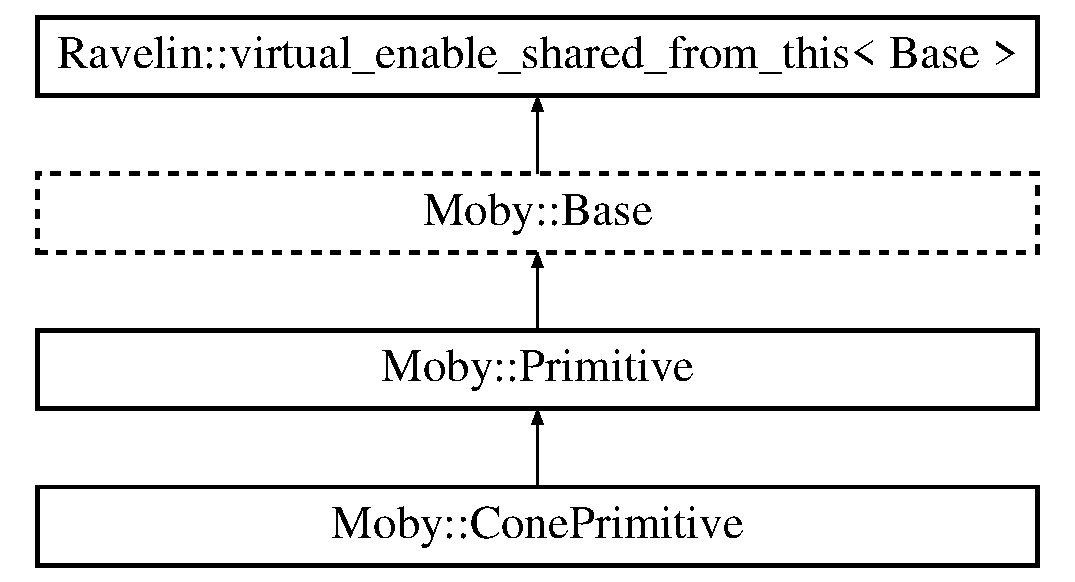
\includegraphics[height=4.000000cm]{classMoby_1_1ConePrimitive}
\end{center}
\end{figure}
\subsection*{Public Member Functions}
\begin{DoxyCompactItemize}
\item 
{\bf Cone\-Primitive} ()\label{classMoby_1_1ConePrimitive_a7e7a6043232e237073e3ffe07135e072}

\begin{DoxyCompactList}\small\item\em Constructs a cone centered at the origin, with the longitudinal axis aligned with the y-\/axis, radius 1.\-0, height 1.\-0, 1 ring and 10 circle points. \end{DoxyCompactList}\item 
{\bf Cone\-Primitive} (double radius, double height)\label{classMoby_1_1ConePrimitive_ada340a7ab2801b710a56e30056acc732}

\begin{DoxyCompactList}\small\item\em Constructs a cone along the y-\/axis with specified radius and height, centered at the origin, with 1 ring and 10 circle points. \end{DoxyCompactList}\item 
{\bfseries Cone\-Primitive} (double radius, double height, unsigned npoints, unsigned nrings, const Ravelin\-::\-Pose3d \&T)\label{classMoby_1_1ConePrimitive_a58ff803e6b380676d86a5bc6b049ee41}

\item 
{\bfseries Cone\-Primitive} (double radius, double height, const Ravelin\-::\-Pose3d \&T)\label{classMoby_1_1ConePrimitive_a20f8169124c41c8a3c5e8dd934ac07db}

\item 
virtual bool {\bf is\-\_\-convex} () const \label{classMoby_1_1ConePrimitive_a5e45656c53f0532b3ac315d58a2c3800}

\begin{DoxyCompactList}\small\item\em Determines whether this primitive is convex. \end{DoxyCompactList}\item 
void {\bf set\-\_\-radius} (double radius)\label{classMoby_1_1ConePrimitive_a5bde5de4ff34f5c6d1e87eca8cff537a}

\begin{DoxyCompactList}\small\item\em Sets the radius for this cone. \end{DoxyCompactList}\item 
void {\bf set\-\_\-height} (double height)\label{classMoby_1_1ConePrimitive_a615e78d4a474b2b4270b6182990fb24a}

\begin{DoxyCompactList}\small\item\em Sets the height for this cone. \end{DoxyCompactList}\item 
void {\bf set\-\_\-circle\-\_\-points} (unsigned n)\label{classMoby_1_1ConePrimitive_a97c846357dcafc281fb024e72e297227}

\begin{DoxyCompactList}\small\item\em Sets the number of points in the rings of the cone. \end{DoxyCompactList}\item 
void {\bf set\-\_\-num\-\_\-rings} (unsigned n)\label{classMoby_1_1ConePrimitive_aadcfd4b1248c4e53167cbe602e757fda}

\begin{DoxyCompactList}\small\item\em Sets the number of rings in the cone. \end{DoxyCompactList}\item 
virtual void {\bf load\-\_\-from\-\_\-xml} (boost\-::shared\-\_\-ptr$<$ const {\bf X\-M\-L\-Tree} $>$ node, std\-::map$<$ std\-::string, {\bf Base\-Ptr} $>$ \&id\-\_\-map)\label{classMoby_1_1ConePrimitive_a5fb7ad4ce31f041a8933cb67e30c3c8b}

\begin{DoxyCompactList}\small\item\em Implements \doxyref{Base\-::load\-\_\-from\-\_\-xml()}{p.}{classMoby_1_1Base_a98b861c1d615a748b576aa613f17389f} for serialization. \end{DoxyCompactList}\item 
virtual void {\bf save\-\_\-to\-\_\-xml} ({\bf X\-M\-L\-Tree\-Ptr} node, std\-::list$<$ boost\-::shared\-\_\-ptr$<$ const {\bf Base} $>$ $>$ \&shared\-\_\-objects) const \label{classMoby_1_1ConePrimitive_a7cf26ee13c1fe73f766d7dba07b55cda}

\begin{DoxyCompactList}\small\item\em Implements \doxyref{Base\-::save\-\_\-to\-\_\-xml()}{p.}{classMoby_1_1Base_aed64905ca39893d02d1e6c3f03f73aa9} for serialization. \end{DoxyCompactList}\item 
virtual {\bf B\-V\-Ptr} {\bf get\-\_\-\-B\-V\-H\-\_\-root} ({\bf Collision\-Geometry\-Ptr} geom)
\begin{DoxyCompactList}\small\item\em Gets vertices from the primitive. \end{DoxyCompactList}\item 
virtual void {\bf get\-\_\-vertices} (boost\-::shared\-\_\-ptr$<$ const Ravelin\-::\-Pose3d $>$ P, std\-::vector$<$ {\bf Point3d} $>$ \&vertices) const \label{classMoby_1_1ConePrimitive_aa4f41bf896b4d1605c508d11d37506d3}

\begin{DoxyCompactList}\small\item\em Gets vertices from the primitive. \end{DoxyCompactList}\item 
virtual void {\bf set\-\_\-pose} (const Ravelin\-::\-Pose3d \&T)\label{classMoby_1_1ConePrimitive_adaf388fdaf4e7fbe9331c768a6211775}

\begin{DoxyCompactList}\small\item\em Transforms the primitive. \end{DoxyCompactList}\item 
virtual double {\bf calc\-\_\-dist\-\_\-and\-\_\-normal} (const {\bf Point3d} \&point, std\-::vector$<$ Ravelin\-::\-Vector3d $>$ \&normals) const \label{classMoby_1_1ConePrimitive_af1d5f382f63f8cbbb7188b2b8413101e}

\begin{DoxyCompactList}\small\item\em Computes the distance and normal from a point on the primitive. \end{DoxyCompactList}\item 
virtual double {\bf calc\-\_\-signed\-\_\-dist} (boost\-::shared\-\_\-ptr$<$ const {\bf Primitive} $>$ p, {\bf Point3d} \&pthis, {\bf Point3d} \&pp) const \label{classMoby_1_1ConePrimitive_a5082277dcf1f1b16333de5b026809855}

\begin{DoxyCompactList}\small\item\em Computes the signed distance between this and another primitive. \end{DoxyCompactList}\item 
virtual boost\-::shared\-\_\-ptr\\*
$<$ const {\bf Indexed\-Tri\-Array} $>$ {\bf get\-\_\-mesh} (boost\-::shared\-\_\-ptr$<$ const Ravelin\-::\-Pose3d $>$ P)\label{classMoby_1_1ConePrimitive_a21873b1161a88b316087413075913d22}

\begin{DoxyCompactList}\small\item\em Gets the triangle mesh for the cone, computing it if necessary. \end{DoxyCompactList}\item 
virtual osg\-::\-Node $\ast$ {\bf create\-\_\-visualization} ()\label{classMoby_1_1ConePrimitive_a5c73da36a3b61b6cc84f76148bb6db7a}

\begin{DoxyCompactList}\small\item\em Creates the visualization for this primitive. \end{DoxyCompactList}\item 
virtual {\bf Point3d} {\bf get\-\_\-supporting\-\_\-point} (const Ravelin\-::\-Vector3d \&d) const \label{classMoby_1_1ConePrimitive_ae25dcfd230a01bf2f93055f85d4cbc37}

\begin{DoxyCompactList}\small\item\em Gets a supporting point in a particular direction. \end{DoxyCompactList}\item 
virtual double {\bf calc\-\_\-signed\-\_\-dist} (const {\bf Point3d} \&p) const \label{classMoby_1_1ConePrimitive_aa3ab279f08fb4deadb656e008144d89f}

\begin{DoxyCompactList}\small\item\em Computes the signed distance from the cylinder. \end{DoxyCompactList}\item 
virtual double {\bfseries get\-\_\-bounding\-\_\-radius} () const \label{classMoby_1_1ConePrimitive_aecd2fdebaaa7356e9b26a88ecb65613e}

\item 
unsigned {\bf get\-\_\-num\-\_\-rings} () const \label{classMoby_1_1ConePrimitive_a6b6e405185d2eb9fdbcf96567d037b0b}

\begin{DoxyCompactList}\small\item\em Gets the number of rings on the cone. \end{DoxyCompactList}\item 
double {\bf get\-\_\-radius} () const \label{classMoby_1_1ConePrimitive_acdea677cfe6803c65a819a201951b0f9}

\begin{DoxyCompactList}\small\item\em Gets the radius of this cone. \end{DoxyCompactList}\item 
double {\bf get\-\_\-height} () const \label{classMoby_1_1ConePrimitive_ac09f06faad30a5746a88fb3f00fcf2dd}

\begin{DoxyCompactList}\small\item\em Gets the height of this cone. \end{DoxyCompactList}\item 
unsigned {\bf get\-\_\-circle\-\_\-points} () const \label{classMoby_1_1ConePrimitive_a819203cb8e6a8e38dba3aebe36738458}

\begin{DoxyCompactList}\small\item\em Gets the number of points in a circle on the cone. \end{DoxyCompactList}\end{DoxyCompactItemize}
\subsection*{Additional Inherited Members}


\subsection{Detailed Description}
Defines a cone primitive. 

The axis of the untransformed cone lies along the global Y-\/axis, and the center of the cone is coincident with the global origin. 

\subsection{Member Function Documentation}
\index{Moby\-::\-Cone\-Primitive@{Moby\-::\-Cone\-Primitive}!get\-\_\-\-B\-V\-H\-\_\-root@{get\-\_\-\-B\-V\-H\-\_\-root}}
\index{get\-\_\-\-B\-V\-H\-\_\-root@{get\-\_\-\-B\-V\-H\-\_\-root}!Moby::ConePrimitive@{Moby\-::\-Cone\-Primitive}}
\subsubsection[{get\-\_\-\-B\-V\-H\-\_\-root}]{\setlength{\rightskip}{0pt plus 5cm}{\bf B\-V\-Ptr} Cone\-Primitive\-::get\-\_\-\-B\-V\-H\-\_\-root (
\begin{DoxyParamCaption}
\item[{{\bf Collision\-Geometry\-Ptr}}]{geom}
\end{DoxyParamCaption}
)\hspace{0.3cm}{\ttfamily [virtual]}}\label{classMoby_1_1ConePrimitive_a6c6f49d922bce62f4d1dccf3fe5ddb9a}


Gets vertices from the primitive. 

Gets the \doxyref{O\-B\-B}{p.}{classMoby_1_1OBB} 

Implements {\bf Moby\-::\-Primitive} \doxyref{}{p.}{classMoby_1_1Primitive_a2c9a61ca714a7b1ac6bc8ae2d9956510}.



References Moby\-::\-Primitive\-::get\-\_\-pose().



The documentation for this class was generated from the following files\-:\begin{DoxyCompactItemize}
\item 
/home/drum/\-Moby/include/\-Moby/Cone\-Primitive.\-h\item 
/home/drum/\-Moby/src/Cone\-Primitive.\-cpp\end{DoxyCompactItemize}

\section{Moby\-:\-:Constraint\-Simulator Class Reference}
\label{classMoby_1_1ConstraintSimulator}\index{Moby\-::\-Constraint\-Simulator@{Moby\-::\-Constraint\-Simulator}}


An virtual class for simulation with constraints.  




{\ttfamily \#include $<$Constraint\-Simulator.\-h$>$}

Inheritance diagram for Moby\-:\-:Constraint\-Simulator\-:\begin{figure}[H]
\begin{center}
\leavevmode
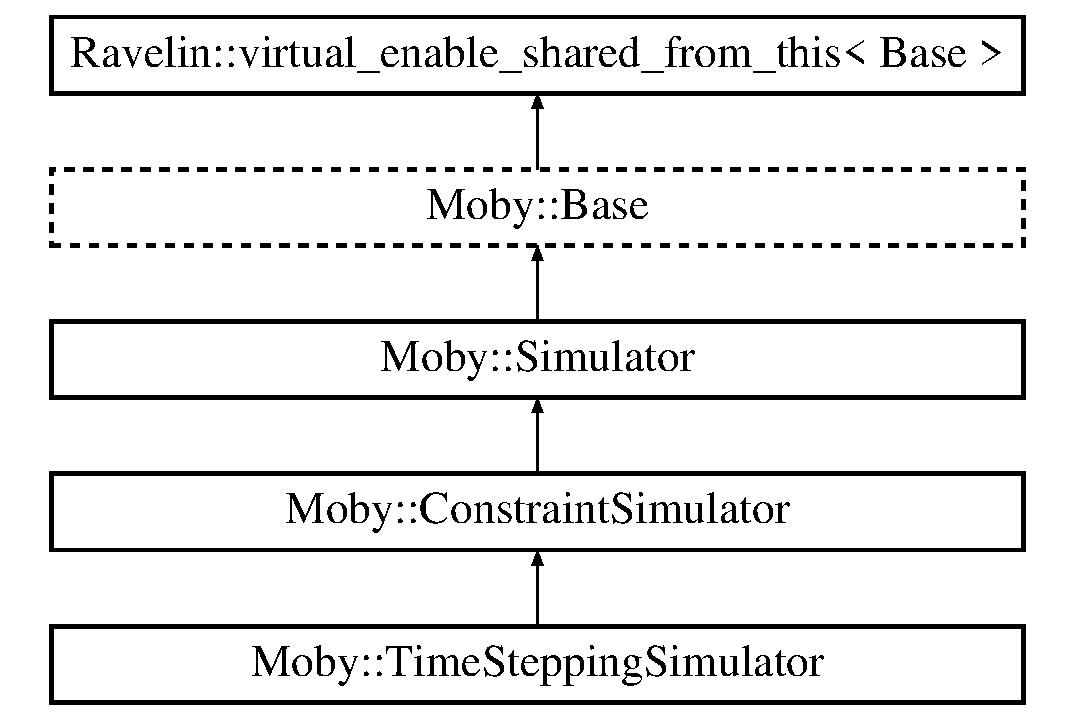
\includegraphics[height=5.000000cm]{classMoby_1_1ConstraintSimulator}
\end{center}
\end{figure}
\subsection*{Public Member Functions}
\begin{DoxyCompactItemize}
\item 
{\bf Constraint\-Simulator} ()\label{classMoby_1_1ConstraintSimulator_aedbfa53caf8953267ea8045841c3aa34}

\begin{DoxyCompactList}\small\item\em Default constructor. \end{DoxyCompactList}\item 
virtual void {\bf load\-\_\-from\-\_\-xml} (boost\-::shared\-\_\-ptr$<$ const {\bf X\-M\-L\-Tree} $>$ node, std\-::map$<$ std\-::string, {\bf Base\-Ptr} $>$ \&id\-\_\-map)\label{classMoby_1_1ConstraintSimulator_aea925f7a62d28833ec377e7176bcca78}

\begin{DoxyCompactList}\small\item\em Implements \doxyref{Base\-::load\-\_\-from\-\_\-xml()}{p.}{classMoby_1_1Base_a98b861c1d615a748b576aa613f17389f} \end{DoxyCompactList}\item 
virtual void {\bf save\-\_\-to\-\_\-xml} ({\bf X\-M\-L\-Tree\-Ptr} node, std\-::list$<$ boost\-::shared\-\_\-ptr$<$ const {\bf Base} $>$ $>$ \&shared\-\_\-objects) const \label{classMoby_1_1ConstraintSimulator_aa97902317a931eb41b6e67069aa3c236}

\begin{DoxyCompactList}\small\item\em Implements \doxyref{Base\-::save\-\_\-to\-\_\-xml()}{p.}{classMoby_1_1Base_aed64905ca39893d02d1e6c3f03f73aa9} \end{DoxyCompactList}\item 
boost\-::shared\-\_\-ptr\\*
$<$ {\bf Contact\-Parameters} $>$ {\bf get\-\_\-contact\-\_\-parameters} ({\bf Collision\-Geometry\-Ptr} geom1, {\bf Collision\-Geometry\-Ptr} geom2) const 
\begin{DoxyCompactList}\small\item\em Gets the contact data between a pair of geometries (if any) \end{DoxyCompactList}\item 
const std\-::vector\\*
$<$ {\bf Pairwise\-Dist\-Info} $>$ \& {\bfseries get\-\_\-pairwise\-\_\-distances} () const \label{classMoby_1_1ConstraintSimulator_a1e22560c8e48a696a627a254bc131267}

\item 
std\-::vector\\*
$<$ {\bf Unilateral\-Constraint} $>$ \& {\bf get\-\_\-compliant\-\_\-constraints} ()\label{classMoby_1_1ConstraintSimulator_a7ce2f9725e1f96f41dcdb4452a0b2d44}

\begin{DoxyCompactList}\small\item\em Gets the (sorted) compliant constraint data. \end{DoxyCompactList}\item 
std\-::vector\\*
$<$ {\bf Unilateral\-Constraint} $>$ \& {\bf get\-\_\-rigid\-\_\-constraints} ()\label{classMoby_1_1ConstraintSimulator_af492f176bd01f46348049ffdef756a72}

\begin{DoxyCompactList}\small\item\em Gets the (sorted) rigid constraint data. \end{DoxyCompactList}\item 
boost\-::shared\-\_\-ptr\\*
$<$ {\bf Collision\-Detection} $>$ {\bf get\-\_\-collision\-\_\-detection} () const \label{classMoby_1_1ConstraintSimulator_abce5ddbc330b074c6c3893fccb4b22c7}

\begin{DoxyCompactList}\small\item\em Gets the collision detection mechanism. \end{DoxyCompactList}\end{DoxyCompactItemize}
\subsection*{Public Attributes}
\begin{DoxyCompactItemize}
\item 
{\bf Constraint\-Stabilization} {\bf cstab}\label{classMoby_1_1ConstraintSimulator_a7fd2315bffefddbc4395d413f60814a2}

\begin{DoxyCompactList}\small\item\em The constraint stabilization mechanism. \end{DoxyCompactList}\item 
std\-::set$<$ Ravelin\-::sorted\-\_\-pair\\*
$<$ {\bf Collision\-Geometry\-Ptr} $>$ $>$ {\bf unchecked\-\_\-pairs}\label{classMoby_1_1ConstraintSimulator_a706d9def5b4e10f8cd4e6f85b4cfc4d7}

\begin{DoxyCompactList}\small\item\em Determines whether two geometries are not checked. \end{DoxyCompactList}\item 
std\-::vector$<$ std\-::pair\\*
$<$ {\bf Controlled\-Body\-Ptr}, \\*
Ravelin\-::\-Vector\-Nd $>$ $>$ {\bf \-\_\-x0}\label{classMoby_1_1ConstraintSimulator_a631b00c84884499fffeffa568a304d94}

\begin{DoxyCompactList}\small\item\em Vectors set and passed to collision detection. \end{DoxyCompactList}\item 
std\-::vector$<$ std\-::pair\\*
$<$ {\bf Controlled\-Body\-Ptr}, \\*
Ravelin\-::\-Vector\-Nd $>$ $>$ {\bfseries \-\_\-x1}\label{classMoby_1_1ConstraintSimulator_a873f6b7a5e8ae98d8bd394243ec7eb77}

\item 
boost\-::shared\-\_\-ptr\\*
$<$ {\bf Contact\-Parameters} $>$($\ast$ {\bf get\-\_\-contact\-\_\-parameters\-\_\-callback\-\_\-fn} )({\bf Collision\-Geometry\-Ptr} g1, {\bf Collision\-Geometry\-Ptr} g2)\label{classMoby_1_1ConstraintSimulator_a03040cb619a75188341b5294ff7b191e}

\begin{DoxyCompactList}\small\item\em Callback function for getting contact parameters. \end{DoxyCompactList}\item 
void($\ast$ {\bf post\-\_\-mini\-\_\-step\-\_\-callback\-\_\-fn} )({\bf Constraint\-Simulator} $\ast$s)\label{classMoby_1_1ConstraintSimulator_aae799e90389294ab8b760fe7f8fcd084}

\begin{DoxyCompactList}\small\item\em Callback function after a mini-\/step is completed. \end{DoxyCompactList}\item 
void($\ast$ {\bf constraint\-\_\-callback\-\_\-fn} )(std\-::vector$<$ {\bf Unilateral\-Constraint} $>$ \&, boost\-::shared\-\_\-ptr$<$ void $>$)
\begin{DoxyCompactList}\small\item\em The callback function (called when constraints have been determined) \end{DoxyCompactList}\item 
void($\ast$ {\bf constraint\-\_\-post\-\_\-callback\-\_\-fn} )(const std\-::vector$<$ {\bf Unilateral\-Constraint} $>$ \&, boost\-::shared\-\_\-ptr$<$ void $>$)\label{classMoby_1_1ConstraintSimulator_aa0442c2de79fba335920e39949617483}

\begin{DoxyCompactList}\small\item\em The callback function (called after forces/impulses are applied) \end{DoxyCompactList}\item 
boost\-::shared\-\_\-ptr$<$ void $>$ {\bf constraint\-\_\-callback\-\_\-data}\label{classMoby_1_1ConstraintSimulator_aee2a305b9783b4df880bc9359244fe46}

\begin{DoxyCompactList}\small\item\em Data passed to unilateral constraint callback. \end{DoxyCompactList}\item 
boost\-::shared\-\_\-ptr$<$ void $>$ {\bf constraint\-\_\-post\-\_\-callback\-\_\-data}\label{classMoby_1_1ConstraintSimulator_afc24fa5f9ccea2c4ae789f4ddd5ae740}

\begin{DoxyCompactList}\small\item\em Data passed to post-\/constraint callback. \end{DoxyCompactList}\item 
std\-::map$<$ Ravelin\-::sorted\-\_\-pair\\*
$<$ {\bf Base\-Ptr} $>$, boost\-::shared\-\_\-ptr\\*
$<$ {\bf Contact\-Parameters} $>$ $>$ {\bf contact\-\_\-params}\label{classMoby_1_1ConstraintSimulator_a03f642db0af706d0e8e5109740853aaa}

\begin{DoxyCompactList}\small\item\em Mapping from objects to contact parameters. \end{DoxyCompactList}\item 
bool {\bf render\-\_\-contact\-\_\-points}\label{classMoby_1_1ConstraintSimulator_a62ea3e938d2119f47ba8a1d778802526}

\begin{DoxyCompactList}\small\item\em If set to 'true' simulator will process contact points for rendering. \end{DoxyCompactList}\end{DoxyCompactItemize}
\subsection*{Protected Member Functions}
\begin{DoxyCompactItemize}
\item 
void {\bf calc\-\_\-impacting\-\_\-unilateral\-\_\-constraint\-\_\-forces} (double dt)\label{classMoby_1_1ConstraintSimulator_ae2492e921775f0b523d4c3e2939d1d83}

\begin{DoxyCompactList}\small\item\em Handles constraints. \end{DoxyCompactList}\item 
void {\bf find\-\_\-unilateral\-\_\-constraints} ()\label{classMoby_1_1ConstraintSimulator_a7fd1a19da75d2726b825e4c2b2bcb577}

\begin{DoxyCompactList}\small\item\em Finds the set of unilateral constraints. \end{DoxyCompactList}\item 
void {\bf calc\-\_\-compliant\-\_\-unilateral\-\_\-constraint\-\_\-forces} ()\label{classMoby_1_1ConstraintSimulator_ad04440352af48ed253da7542b4ac7de7}

\begin{DoxyCompactList}\small\item\em Computes compliant contact forces. \end{DoxyCompactList}\item 
void {\bf preprocess\-\_\-constraint} ({\bf Unilateral\-Constraint} \&e)\label{classMoby_1_1ConstraintSimulator_a35cc1ffe2396ab87b6365beeb799a139}

\begin{DoxyCompactList}\small\item\em Performs necessary preprocessing on an constraint. \end{DoxyCompactList}\item 
void {\bf determine\-\_\-geometries} ()\label{classMoby_1_1ConstraintSimulator_abcaaf895ef05ecfe7c518f9b40f8f807}

\begin{DoxyCompactList}\small\item\em Sets up the list of collision geometries. \end{DoxyCompactList}\item 
void {\bf broad\-\_\-phase} (double dt)\label{classMoby_1_1ConstraintSimulator_a2356991bba83552dea0c6143c0161a7c}

\begin{DoxyCompactList}\small\item\em Does broad phase collision detection, identifying which pairs of geometries may come into contact over time step of dt. \end{DoxyCompactList}\item 
void {\bf calc\-\_\-pairwise\-\_\-distances} ()
\begin{DoxyCompactList}\small\item\em Computes pairwise distances of geometries at their current poses, using broad phase results to determine which pairs should be checked. \end{DoxyCompactList}\item 
void {\bf visualize\-\_\-contact} ({\bf Unilateral\-Constraint} \&constraint)\label{classMoby_1_1ConstraintSimulator_a8b1b58be1d7c22278f7fe233b8ef3598}

\begin{DoxyCompactList}\small\item\em Draws a ray directed from a contact point along the contact normal. \end{DoxyCompactList}\item 
double {\bfseries calc\-\_\-\-C\-A\-\_\-step} ()\label{classMoby_1_1ConstraintSimulator_a99ec1d3bd1dcab394b056b21cb5a4952}

\item 
double {\bfseries calc\-\_\-next\-\_\-\-C\-A\-\_\-\-Euler\-\_\-step} (double contact\-\_\-dist\-\_\-thresh) const \label{classMoby_1_1ConstraintSimulator_a08fbad5eb724574d2fb27a6743f5f9d4}

\end{DoxyCompactItemize}
\subsection*{Protected Attributes}
\begin{DoxyCompactItemize}
\item 
{\bf Impact\-Constraint\-Handler} {\bf \-\_\-impact\-\_\-constraint\-\_\-handler}\label{classMoby_1_1ConstraintSimulator_a80817dedc873e645f6917744095968fc}

\begin{DoxyCompactList}\small\item\em Object for handling impact constraints. \end{DoxyCompactList}\item 
{\bf Penalty\-Constraint\-Handler} {\bf \-\_\-penalty\-\_\-constraint\-\_\-handler}\label{classMoby_1_1ConstraintSimulator_aca16b7cfc19c13d07914fd33e8167907}

\begin{DoxyCompactList}\small\item\em Object for handling penalty constraints. \end{DoxyCompactList}\item 
std\-::vector$<$ {\bf Unilateral\-Constraint} $>$ {\bf \-\_\-rigid\-\_\-constraints}\label{classMoby_1_1ConstraintSimulator_ac363fa58326b6a110c1ec2008fd4b15d}

\begin{DoxyCompactList}\small\item\em The vector of rigid constraints. \end{DoxyCompactList}\item 
std\-::vector$<$ {\bf Unilateral\-Constraint} $>$ {\bf \-\_\-compliant\-\_\-constraints}\label{classMoby_1_1ConstraintSimulator_adba24b0d87ec90a252674e5201905dd0}

\begin{DoxyCompactList}\small\item\em The vector of compliant constraints. \end{DoxyCompactList}\item 
std\-::vector$<$ {\bf Pairwise\-Dist\-Info} $>$ {\bf \-\_\-pairwise\-\_\-distances}\label{classMoby_1_1ConstraintSimulator_a62066a08ab5002a5acccd3ab9a47be5c}

\begin{DoxyCompactList}\small\item\em Pairwise distances at bodies' current configurations. \end{DoxyCompactList}\item 
Ravelin\-::\-Vector\-Nd {\bf \-\_\-work\-V}\label{classMoby_1_1ConstraintSimulator_a29b926f0ab32d7258118d35eb9a2a226}

\begin{DoxyCompactList}\small\item\em Work vector. \end{DoxyCompactList}\item 
boost\-::shared\-\_\-ptr\\*
$<$ {\bf Collision\-Detection} $>$ {\bf \-\_\-coldet}\label{classMoby_1_1ConstraintSimulator_a473a4b5c73c3dc7e1478cfa918bedb68}

\begin{DoxyCompactList}\small\item\em The collision detection mechanism. \end{DoxyCompactList}\item 
std\-::vector$<$ {\bf Collision\-Geometry\-Ptr} $>$ {\bf \-\_\-geometries}\label{classMoby_1_1ConstraintSimulator_a1c0af7852e337d3c63f8f689fc353dc4}

\begin{DoxyCompactList}\small\item\em The geometries in the simulator. \end{DoxyCompactList}\item 
std\-::vector$<$ std\-::pair\\*
$<$ {\bf Collision\-Geometry\-Ptr}, \\*
{\bf Collision\-Geometry\-Ptr} $>$ $>$ {\bf \-\_\-pairs\-\_\-to\-\_\-check}\label{classMoby_1_1ConstraintSimulator_a08f8423e1453a35ff68f18c0a4572b5b}

\begin{DoxyCompactList}\small\item\em Geometric pairs that should be checked for unilateral constraints (according to broad phase collision detection) \end{DoxyCompactList}\end{DoxyCompactItemize}
\subsection*{Friends}
\begin{DoxyCompactItemize}
\item 
class {\bfseries Collision\-Detection}\label{classMoby_1_1ConstraintSimulator_aa87aa6084db35876513fcb4fdd4427ac}

\item 
class {\bfseries Constraint\-Stabilization}\label{classMoby_1_1ConstraintSimulator_a320e2b5d0cb83071af150f47d50ca127}

\end{DoxyCompactItemize}
\subsection*{Additional Inherited Members}


\subsection{Detailed Description}
An virtual class for simulation with constraints. 

\subsection{Member Function Documentation}
\index{Moby\-::\-Constraint\-Simulator@{Moby\-::\-Constraint\-Simulator}!calc\-\_\-pairwise\-\_\-distances@{calc\-\_\-pairwise\-\_\-distances}}
\index{calc\-\_\-pairwise\-\_\-distances@{calc\-\_\-pairwise\-\_\-distances}!Moby::ConstraintSimulator@{Moby\-::\-Constraint\-Simulator}}
\subsubsection[{calc\-\_\-pairwise\-\_\-distances}]{\setlength{\rightskip}{0pt plus 5cm}void Constraint\-Simulator\-::calc\-\_\-pairwise\-\_\-distances (
\begin{DoxyParamCaption}
{}
\end{DoxyParamCaption}
)\hspace{0.3cm}{\ttfamily [protected]}}\label{classMoby_1_1ConstraintSimulator_aef9eb2121d39d21eaae43bfe65e770b6}


Computes pairwise distances of geometries at their current poses, using broad phase results to determine which pairs should be checked. 


\begin{DoxyParams}{Parameters}
{\em pairwise\-\_\-distances} & on return, contains the pairwise distances \\
\hline
\end{DoxyParams}
\index{Moby\-::\-Constraint\-Simulator@{Moby\-::\-Constraint\-Simulator}!get\-\_\-contact\-\_\-parameters@{get\-\_\-contact\-\_\-parameters}}
\index{get\-\_\-contact\-\_\-parameters@{get\-\_\-contact\-\_\-parameters}!Moby::ConstraintSimulator@{Moby\-::\-Constraint\-Simulator}}
\subsubsection[{get\-\_\-contact\-\_\-parameters}]{\setlength{\rightskip}{0pt plus 5cm}shared\-\_\-ptr$<$ {\bf Contact\-Parameters} $>$ Constraint\-Simulator\-::get\-\_\-contact\-\_\-parameters (
\begin{DoxyParamCaption}
\item[{{\bf Collision\-Geometry\-Ptr}}]{geom1, }
\item[{{\bf Collision\-Geometry\-Ptr}}]{geom2}
\end{DoxyParamCaption}
) const}\label{classMoby_1_1ConstraintSimulator_a9657a9a8b0c9c819bb0e635f93cfebf5}


Gets the contact data between a pair of geometries (if any) 

This method looks for contact data not only between the pair of geometries, but also the rigid bodies that the geometries belong to, and any articulated bodies as well. The search proceeds in the following manner\-: \par
 
\begin{DoxyEnumerate}
\item two collision geometries 
\item one collision geometry, one rigid body 
\item two rigid bodies 
\item one collision geometry, one articulated body 
\item one rigid body, one articulated body 
\item two articulated bodies 
\end{DoxyEnumerate}The search order allows for multiple granularities; for example, a collision can easily be specified between two geometries of two of a robot's links (i.\-e., representing different surfaces on the links), between two links, or between two robots. 
\begin{DoxyParams}{Parameters}
{\em g1} & the first collision geometry \\
\hline
{\em g2} & the second collision geometry \\
\hline
\end{DoxyParams}
\begin{DoxyReturn}{Returns}
a pointer to the contact data, if any, found 
\end{DoxyReturn}


\subsection{Member Data Documentation}
\index{Moby\-::\-Constraint\-Simulator@{Moby\-::\-Constraint\-Simulator}!constraint\-\_\-callback\-\_\-fn@{constraint\-\_\-callback\-\_\-fn}}
\index{constraint\-\_\-callback\-\_\-fn@{constraint\-\_\-callback\-\_\-fn}!Moby::ConstraintSimulator@{Moby\-::\-Constraint\-Simulator}}
\subsubsection[{constraint\-\_\-callback\-\_\-fn}]{\setlength{\rightskip}{0pt plus 5cm}void($\ast$ Moby\-::\-Constraint\-Simulator\-::constraint\-\_\-callback\-\_\-fn)(std\-::vector$<$ {\bf Unilateral\-Constraint} $>$ \&, boost\-::shared\-\_\-ptr$<$ void $>$)}\label{classMoby_1_1ConstraintSimulator_a6435646bf05f3a9ae769ea240bdcadf0}


The callback function (called when constraints have been determined) 

The callback function can remove constraints from the list, which will disable their processing (however, doing so may prevent the simulation from making progress, as the simulator attempts to disallow violations. 

The documentation for this class was generated from the following files\-:\begin{DoxyCompactItemize}
\item 
/home/drum/\-Moby/include/\-Moby/Constraint\-Simulator.\-h\item 
/home/drum/\-Moby/src/Constraint\-Simulator.\-cpp\end{DoxyCompactItemize}

\section{Moby\-:\-:Constraint\-Stabilization Class Reference}
\label{classMoby_1_1ConstraintStabilization}\index{Moby\-::\-Constraint\-Stabilization@{Moby\-::\-Constraint\-Stabilization}}


Projected constraint stabilization mechanism.  




{\ttfamily \#include $<$Constraint\-Stabilization.\-h$>$}

\subsection*{Public Member Functions}
\begin{DoxyCompactItemize}
\item 
void {\bf stabilize} (boost\-::shared\-\_\-ptr$<$ {\bf Constraint\-Simulator} $>$ sim)\label{classMoby_1_1ConstraintStabilization_a0e32da79f7bcbf9bb07a2ce0f3c01fff}

\begin{DoxyCompactList}\small\item\em Stabilizes the constraints in the simulator. \end{DoxyCompactList}\end{DoxyCompactItemize}
\subsection*{Public Attributes}
\begin{DoxyCompactItemize}
\item 
double {\bfseries eps}\label{classMoby_1_1ConstraintStabilization_a8f4643aff43cb4ad52e44086a18ce67c}

\item 
double {\bfseries bilateral\-\_\-eps}\label{classMoby_1_1ConstraintStabilization_a0779a49fc72a73df64bac7f75b49a368}

\item 
unsigned {\bfseries max\-\_\-iterations}\label{classMoby_1_1ConstraintStabilization_a31a8459ca9351c79a9ce4e65aeb9cf1a}

\end{DoxyCompactItemize}


\subsection{Detailed Description}
Projected constraint stabilization mechanism. 

The documentation for this class was generated from the following files\-:\begin{DoxyCompactItemize}
\item 
/home/drum/\-Moby/include/\-Moby/Constraint\-Stabilization.\-h\item 
/home/drum/\-Moby/src/Constraint\-Stabilization.\-cpp\end{DoxyCompactItemize}

\section{Moby\-:\-:Contact\-Parameters Class Reference}
\label{classMoby_1_1ContactParameters}\index{Moby\-::\-Contact\-Parameters@{Moby\-::\-Contact\-Parameters}}


Class for storing contact modeling parameters between two bodies.  




{\ttfamily \#include $<$Contact\-Parameters.\-h$>$}

Inheritance diagram for Moby\-:\-:Contact\-Parameters\-:\begin{figure}[H]
\begin{center}
\leavevmode
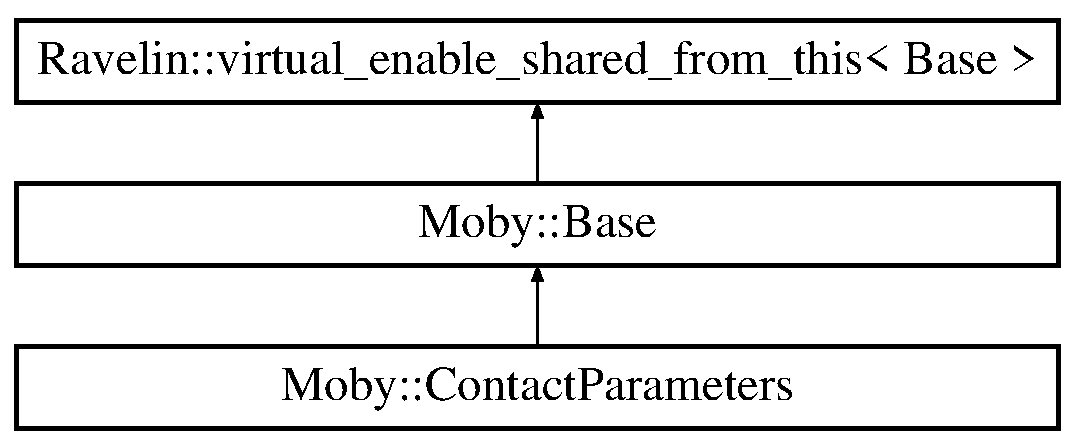
\includegraphics[height=3.000000cm]{classMoby_1_1ContactParameters}
\end{center}
\end{figure}
\subsection*{Public Member Functions}
\begin{DoxyCompactItemize}
\item 
{\bf Contact\-Parameters} ()
\begin{DoxyCompactList}\small\item\em Constructs a \doxyref{Contact\-Parameters}{p.}{classMoby_1_1ContactParameters} object with no object pointers. \end{DoxyCompactList}\item 
{\bf Contact\-Parameters} ({\bf Base\-Ptr} o1, {\bf Base\-Ptr} o2)
\begin{DoxyCompactList}\small\item\em Constructs a \doxyref{Contact\-Parameters}{p.}{classMoby_1_1ContactParameters} object with the given object I\-Ds. \end{DoxyCompactList}\item 
virtual void {\bf load\-\_\-from\-\_\-xml} (boost\-::shared\-\_\-ptr$<$ const {\bf X\-M\-L\-Tree} $>$ node, std\-::map$<$ std\-::string, {\bf Base\-Ptr} $>$ \&id\-\_\-map)
\begin{DoxyCompactList}\small\item\em Implements \doxyref{Base\-::load\-\_\-from\-\_\-xml()}{p.}{classMoby_1_1Base_a98b861c1d615a748b576aa613f17389f} \end{DoxyCompactList}\item 
virtual void {\bf save\-\_\-to\-\_\-xml} ({\bf X\-M\-L\-Tree\-Ptr} node, std\-::list$<$ boost\-::shared\-\_\-ptr$<$ const {\bf Base} $>$ $>$ \&shared\-\_\-objects) const 
\end{DoxyCompactItemize}
\subsection*{Public Attributes}
\begin{DoxyCompactItemize}
\item 
Ravelin\-::sorted\-\_\-pair$<$ {\bf Base\-Ptr} $>$ {\bf objects}\label{classMoby_1_1ContactParameters_ac41104e5f3bb749fd4c0c3ab52d8bd90}

\begin{DoxyCompactList}\small\item\em The objects in contact. \end{DoxyCompactList}\item 
double {\bf epsilon}\label{classMoby_1_1ContactParameters_aac5600571c18d712f29597cd1bf79667}

\begin{DoxyCompactList}\small\item\em Coefficient of restitution for contact (default is 0.\-0) \end{DoxyCompactList}\item 
double {\bf mu\-\_\-coulomb}\label{classMoby_1_1ContactParameters_a2811ce2dc1af06d8e64e0fce66f371d4}

\begin{DoxyCompactList}\small\item\em Coefficient of Coulomb friction for contact (default is 0.\-0) \end{DoxyCompactList}\item 
double {\bf mu\-\_\-viscous}\label{classMoby_1_1ContactParameters_a5220ad24cf8380c8575e352ba210ecd0}

\begin{DoxyCompactList}\small\item\em Coefficient of viscous friction for contact (default is 0.\-0) \end{DoxyCompactList}\item 
double {\bf stiffness}\label{classMoby_1_1ContactParameters_a229814989a7310f8f6a8bad6d579237f}

\begin{DoxyCompactList}\small\item\em contact stiffness (set to zero stiffness for true rigidity) \end{DoxyCompactList}\item 
double {\bf damping}\label{classMoby_1_1ContactParameters_a869398662abf9768886cc72f4ab8ab56}

\begin{DoxyCompactList}\small\item\em contact damping \end{DoxyCompactList}\item 
double {\bf penalty\-\_\-\-Kp}\label{classMoby_1_1ContactParameters_a3972b61941226000594d5513bfc4b7f5}

\begin{DoxyCompactList}\small\item\em Penalty Method Depth Penalty. \end{DoxyCompactList}\item 
double {\bf penalty\-\_\-\-Kv}\label{classMoby_1_1ContactParameters_a890d14656d01524b7dc1b366cc2f091c}

\begin{DoxyCompactList}\small\item\em Penalty Method Interpenetration Speed. \end{DoxyCompactList}\item 
unsigned {\bf N\-K}\label{classMoby_1_1ContactParameters_aee34bedcbf0b6af0359b9a970f54532f}

\begin{DoxyCompactList}\small\item\em Number of edges in the polygon friction cone, minimum of 4 (default 4) \end{DoxyCompactList}\end{DoxyCompactItemize}
\subsection*{Additional Inherited Members}


\subsection{Detailed Description}
Class for storing contact modeling parameters between two bodies. 

\subsection{Constructor \& Destructor Documentation}
\index{Moby\-::\-Contact\-Parameters@{Moby\-::\-Contact\-Parameters}!Contact\-Parameters@{Contact\-Parameters}}
\index{Contact\-Parameters@{Contact\-Parameters}!Moby::ContactParameters@{Moby\-::\-Contact\-Parameters}}
\subsubsection[{Contact\-Parameters}]{\setlength{\rightskip}{0pt plus 5cm}Contact\-Parameters\-::\-Contact\-Parameters (
\begin{DoxyParamCaption}
{}
\end{DoxyParamCaption}
)}\label{classMoby_1_1ContactParameters_a6c65cec9b290adf9a00ea509767b7419}


Constructs a \doxyref{Contact\-Parameters}{p.}{classMoby_1_1ContactParameters} object with no object pointers. 

All gains and coefficients are set to zero. \index{Moby\-::\-Contact\-Parameters@{Moby\-::\-Contact\-Parameters}!Contact\-Parameters@{Contact\-Parameters}}
\index{Contact\-Parameters@{Contact\-Parameters}!Moby::ContactParameters@{Moby\-::\-Contact\-Parameters}}
\subsubsection[{Contact\-Parameters}]{\setlength{\rightskip}{0pt plus 5cm}Contact\-Parameters\-::\-Contact\-Parameters (
\begin{DoxyParamCaption}
\item[{{\bf Base\-Ptr}}]{o1, }
\item[{{\bf Base\-Ptr}}]{o2}
\end{DoxyParamCaption}
)}\label{classMoby_1_1ContactParameters_a14778aeeb916223d1828fd845a0eacc2}


Constructs a \doxyref{Contact\-Parameters}{p.}{classMoby_1_1ContactParameters} object with the given object I\-Ds. 

All gains and coefficients are set to zero. 

\subsection{Member Function Documentation}
\index{Moby\-::\-Contact\-Parameters@{Moby\-::\-Contact\-Parameters}!load\-\_\-from\-\_\-xml@{load\-\_\-from\-\_\-xml}}
\index{load\-\_\-from\-\_\-xml@{load\-\_\-from\-\_\-xml}!Moby::ContactParameters@{Moby\-::\-Contact\-Parameters}}
\subsubsection[{load\-\_\-from\-\_\-xml}]{\setlength{\rightskip}{0pt plus 5cm}void Contact\-Parameters\-::load\-\_\-from\-\_\-xml (
\begin{DoxyParamCaption}
\item[{boost\-::shared\-\_\-ptr$<$ const {\bf X\-M\-L\-Tree} $>$}]{node, }
\item[{std\-::map$<$ std\-::string, {\bf Base\-Ptr} $>$ \&}]{id\-\_\-map}
\end{DoxyParamCaption}
)\hspace{0.3cm}{\ttfamily [virtual]}}\label{classMoby_1_1ContactParameters_a00c9c5d4c9c1f9a5f8235689de2c590d}


Implements \doxyref{Base\-::load\-\_\-from\-\_\-xml()}{p.}{classMoby_1_1Base_a98b861c1d615a748b576aa613f17389f} 

This method does not read the \doxyref{Base}{p.}{classMoby_1_1Base} information (i.\-e., name()), because a name for this object is unnecessary. 

Reimplemented from {\bf Moby\-::\-Base} \doxyref{}{p.}{classMoby_1_1Base_a98b861c1d615a748b576aa613f17389f}.



References Moby\-::\-X\-M\-L\-Attrib\-::get\-\_\-real\-\_\-value().

\index{Moby\-::\-Contact\-Parameters@{Moby\-::\-Contact\-Parameters}!save\-\_\-to\-\_\-xml@{save\-\_\-to\-\_\-xml}}
\index{save\-\_\-to\-\_\-xml@{save\-\_\-to\-\_\-xml}!Moby::ContactParameters@{Moby\-::\-Contact\-Parameters}}
\subsubsection[{save\-\_\-to\-\_\-xml}]{\setlength{\rightskip}{0pt plus 5cm}void Contact\-Parameters\-::save\-\_\-to\-\_\-xml (
\begin{DoxyParamCaption}
\item[{{\bf X\-M\-L\-Tree\-Ptr}}]{node, }
\item[{std\-::list$<$ boost\-::shared\-\_\-ptr$<$ const {\bf Base} $>$ $>$ \&}]{shared\-\_\-objects}
\end{DoxyParamCaption}
) const\hspace{0.3cm}{\ttfamily [virtual]}}\label{classMoby_1_1ContactParameters_aaa6f5a2f71dab3cb2a2bfd750d8ba0f2}
This method does not write the \doxyref{Base}{p.}{classMoby_1_1Base} information, because neither a name nor a unique I\-D are useful. 

Reimplemented from {\bf Moby\-::\-Base} \doxyref{}{p.}{classMoby_1_1Base_aed64905ca39893d02d1e6c3f03f73aa9}.



The documentation for this class was generated from the following files\-:\begin{DoxyCompactItemize}
\item 
/home/drum/\-Moby/include/\-Moby/Contact\-Parameters.\-h\item 
/home/drum/\-Moby/src/Contact\-Parameters.\-cpp\end{DoxyCompactItemize}

\section{Moby\-:\-:Controlled\-Body Class Reference}
\label{classMoby_1_1ControlledBody}\index{Moby\-::\-Controlled\-Body@{Moby\-::\-Controlled\-Body}}


Superclass for controlled bodies.  




{\ttfamily \#include $<$Controlled\-Body.\-h$>$}

Inheritance diagram for Moby\-:\-:Controlled\-Body\-:\begin{figure}[H]
\begin{center}
\leavevmode
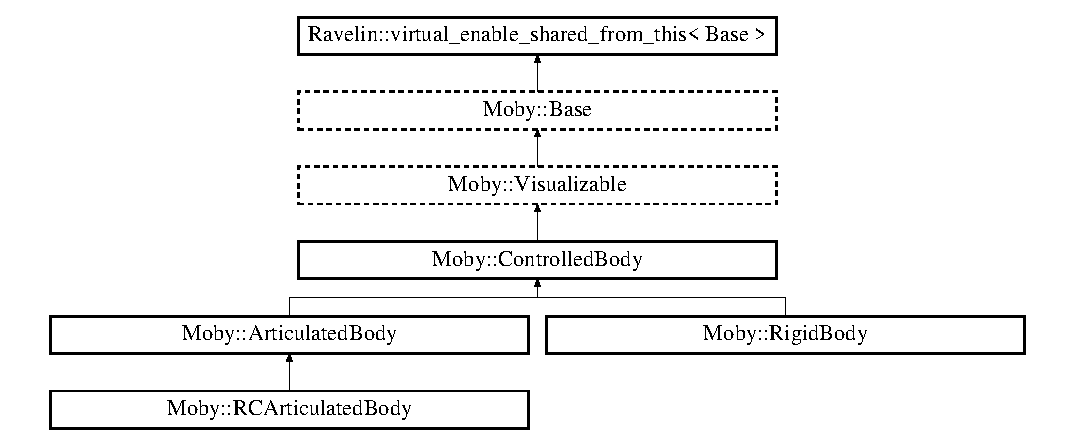
\includegraphics[height=5.526316cm]{classMoby_1_1ControlledBody}
\end{center}
\end{figure}
\subsection*{Public Member Functions}
\begin{DoxyCompactItemize}
\item 
virtual void {\bf load\-\_\-from\-\_\-xml} (boost\-::shared\-\_\-ptr$<$ const {\bf X\-M\-L\-Tree} $>$ node, std\-::map$<$ std\-::string, {\bf Base\-Ptr} $>$ \&id\-\_\-map)\label{classMoby_1_1ControlledBody_aa537fd1b68d720745cd7a7a2580ce9d3}

\begin{DoxyCompactList}\small\item\em Loads the body's state via X\-M\-L. \end{DoxyCompactList}\item 
virtual void {\bf save\-\_\-to\-\_\-xml} ({\bf X\-M\-L\-Tree\-Ptr} node, std\-::list$<$ boost\-::shared\-\_\-ptr$<$ const {\bf Base} $>$ $>$ \&shared\-\_\-objects) const \label{classMoby_1_1ControlledBody_a8652ca9cedf67ee84f29ea004bb1a872}

\begin{DoxyCompactList}\small\item\em Implements \doxyref{Base\-::save\-\_\-to\-\_\-xml()}{p.}{classMoby_1_1Base_aed64905ca39893d02d1e6c3f03f73aa9} \end{DoxyCompactList}\item 
const std\-::list\\*
$<$ {\bf Recurrent\-Force\-Ptr} $>$ \& {\bf get\-\_\-recurrent\-\_\-forces} () const \label{classMoby_1_1ControlledBody_a64e7f87362bcdb718b82f7d30f5d4367}

\begin{DoxyCompactList}\small\item\em Gets the set of recurrent forces applied to this body. \end{DoxyCompactList}\item 
std\-::list$<$ {\bf Recurrent\-Force\-Ptr} $>$ \& {\bf get\-\_\-recurrent\-\_\-forces} ()\label{classMoby_1_1ControlledBody_a872a0c7e78528cfc3dceae7491397384}

\begin{DoxyCompactList}\small\item\em Gets the set of recurrent forces applied to this body. \end{DoxyCompactList}\item 
virtual void {\bf prepare\-\_\-to\-\_\-calc\-\_\-ode\-\_\-sustained\-\_\-constraints} (Ravelin\-::\-Shared\-Const\-Vector\-Nd \&x, double t, double dt, void $\ast$data)=0\label{classMoby_1_1ControlledBody_a6df8a844762bcc3cacd27b21e1e3b0c9}

\begin{DoxyCompactList}\small\item\em Prepares to compute the derivative of the body (sustained constraints) \end{DoxyCompactList}\item 
virtual void {\bf prepare\-\_\-to\-\_\-calc\-\_\-ode} (Ravelin\-::\-Shared\-Const\-Vector\-Nd \&x, double t, double dt, void $\ast$data)=0\label{classMoby_1_1ControlledBody_aa1b930c7402320aee050f6867bd53ef7}

\begin{DoxyCompactList}\small\item\em Prepares to compute the derivative of the body. \end{DoxyCompactList}\item 
virtual void {\bf ode} (double t, double dt, void $\ast$data, Ravelin\-::\-Shared\-Vector\-Nd \&dx)=0\label{classMoby_1_1ControlledBody_a938883c043d39824b1b2353ecb3752b6}

\begin{DoxyCompactList}\small\item\em Computes the derivative of the body. \end{DoxyCompactList}\end{DoxyCompactItemize}
\subsection*{Public Attributes}
\begin{DoxyCompactItemize}
\item 
Ravelin\-::\-Vector\-Nd \&($\ast$ {\bf controller} )(boost\-::shared\-\_\-ptr$<$ {\bf Controlled\-Body} $>$ body, Ravelin\-::\-Vector\-Nd \&, double, void $\ast$)\label{classMoby_1_1ControlledBody_af0f0f287bc6b7201ea2454b180cb7e51}

\begin{DoxyCompactList}\small\item\em The controller callback, if any, for this body. \end{DoxyCompactList}\item 
void $\ast$ {\bf controller\-\_\-arg}\label{classMoby_1_1ControlledBody_a2a8301ec8cd93f152f9a868e531b4f57}

\begin{DoxyCompactList}\small\item\em Argument to be passed to the controller. \end{DoxyCompactList}\end{DoxyCompactItemize}
\subsection*{Protected Attributes}
\begin{DoxyCompactItemize}
\item 
boost\-::weak\-\_\-ptr$<$ {\bf Simulator} $>$ {\bf simulator}\label{classMoby_1_1ControlledBody_ae05a3dda7730a3036867a0726211f078}

\begin{DoxyCompactList}\small\item\em Pointer to the simulator (necessary for applying impulses w/constraints) \end{DoxyCompactList}\end{DoxyCompactItemize}
\subsection*{Friends}
\begin{DoxyCompactItemize}
\item 
class {\bfseries Simulator}\label{classMoby_1_1ControlledBody_a4ba4278eee9a6776d60f4aa6b42c3a76}

\end{DoxyCompactItemize}
\subsection*{Additional Inherited Members}


\subsection{Detailed Description}
Superclass for controlled bodies. 

The documentation for this class was generated from the following files\-:\begin{DoxyCompactItemize}
\item 
/home/drum/\-Moby/include/\-Moby/Controlled\-Body.\-h\item 
/home/drum/\-Moby/src/Controlled\-Body.\-cpp\end{DoxyCompactItemize}

\section{Moby\-:\-:Cylinder\-Primitive Class Reference}
\label{classMoby_1_1CylinderPrimitive}\index{Moby\-::\-Cylinder\-Primitive@{Moby\-::\-Cylinder\-Primitive}}


Defines a cylinder primitive.  




{\ttfamily \#include $<$Cylinder\-Primitive.\-h$>$}

Inheritance diagram for Moby\-:\-:Cylinder\-Primitive\-:\begin{figure}[H]
\begin{center}
\leavevmode
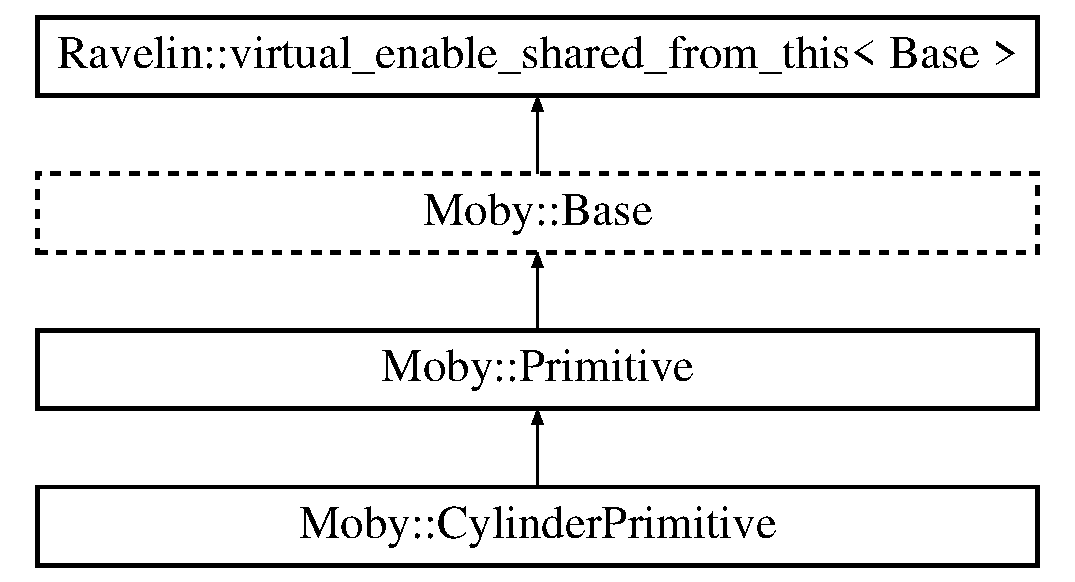
\includegraphics[height=4.000000cm]{classMoby_1_1CylinderPrimitive}
\end{center}
\end{figure}
\subsection*{Public Member Functions}
\begin{DoxyCompactItemize}
\item 
{\bf Cylinder\-Primitive} ()\label{classMoby_1_1CylinderPrimitive_a95a475b49ba2c6b8e07e0ee6a08f9cae}

\begin{DoxyCompactList}\small\item\em Constructs a cylinder centered at the origin, with the longitudinal axis aligned with the y-\/axis, radius 1.\-0, height 1.\-0, 10 circle points, and 2 rings. \end{DoxyCompactList}\item 
{\bf Cylinder\-Primitive} (double radius, double height)\label{classMoby_1_1CylinderPrimitive_ab8ff6b015c8113a91a25df613380ff6e}

\begin{DoxyCompactList}\small\item\em Constructs a cylinder along the y-\/axis with specified radius and height, centered at the origin, with 10 circle points and 2 rings. \end{DoxyCompactList}\item 
{\bfseries Cylinder\-Primitive} (double radius, double height, unsigned n, unsigned nrings, const Ravelin\-::\-Pose3d \&T)\label{classMoby_1_1CylinderPrimitive_a6eb89dcfcf4b6e163fed1adbf27e891b}

\item 
{\bfseries Cylinder\-Primitive} (double radius, double height, const Ravelin\-::\-Pose3d \&T)\label{classMoby_1_1CylinderPrimitive_a7329238ebe6668969c1dcc07cf61d654}

\item 
virtual bool {\bf is\-\_\-convex} () const \label{classMoby_1_1CylinderPrimitive_a028909699862822b0f53b0aa80da2677}

\begin{DoxyCompactList}\small\item\em Determines whether this primitive is convex. \end{DoxyCompactList}\item 
void {\bf set\-\_\-radius} (double radius)\label{classMoby_1_1CylinderPrimitive_aea3d06e1a67321d2ae614be637027613}

\begin{DoxyCompactList}\small\item\em Sets the radius for this cylinder. \end{DoxyCompactList}\item 
void {\bf set\-\_\-height} (double height)\label{classMoby_1_1CylinderPrimitive_a7e52bf96ed47dfc6ac7a78238e4525c9}

\begin{DoxyCompactList}\small\item\em Sets the height for this cylinder. \end{DoxyCompactList}\item 
void {\bf set\-\_\-num\-\_\-circle\-\_\-points} (unsigned n)\label{classMoby_1_1CylinderPrimitive_a3ea640b6a4acbd0af5bfebc0df309041}

\begin{DoxyCompactList}\small\item\em Sets the number of points in the circles of the cylinder. \end{DoxyCompactList}\item 
void {\bf set\-\_\-num\-\_\-rings} (unsigned n)\label{classMoby_1_1CylinderPrimitive_a10a00ff8217f8f799a92a8fe0e686e32}

\begin{DoxyCompactList}\small\item\em Sets the number of rings for determining \char`\"{}virtual points\char`\"{} (points on the tube of the cylinder) \end{DoxyCompactList}\item 
virtual void {\bf set\-\_\-pose} (const Ravelin\-::\-Pose3d \&T)\label{classMoby_1_1CylinderPrimitive_a7a90cb184a9eec9d682da75d544f5c00}

\begin{DoxyCompactList}\small\item\em Transforms the primitive. \end{DoxyCompactList}\item 
virtual void {\bf load\-\_\-from\-\_\-xml} (boost\-::shared\-\_\-ptr$<$ const {\bf X\-M\-L\-Tree} $>$ node, std\-::map$<$ std\-::string, {\bf Base\-Ptr} $>$ \&id\-\_\-map)\label{classMoby_1_1CylinderPrimitive_a8530fa4d6370204c5333e0fe73a570df}

\begin{DoxyCompactList}\small\item\em Implements \doxyref{Base\-::load\-\_\-from\-\_\-xml()}{p.}{classMoby_1_1Base_a98b861c1d615a748b576aa613f17389f} for serialization. \end{DoxyCompactList}\item 
virtual void {\bf save\-\_\-to\-\_\-xml} ({\bf X\-M\-L\-Tree\-Ptr} node, std\-::list$<$ boost\-::shared\-\_\-ptr$<$ const {\bf Base} $>$ $>$ \&shared\-\_\-objects) const \label{classMoby_1_1CylinderPrimitive_acd5e18cdf754052894557d7c84719dfd}

\begin{DoxyCompactList}\small\item\em Implements \doxyref{Base\-::save\-\_\-to\-\_\-xml()}{p.}{classMoby_1_1Base_aed64905ca39893d02d1e6c3f03f73aa9} for serialization. \end{DoxyCompactList}\item 
virtual {\bf B\-V\-Ptr} {\bf get\-\_\-\-B\-V\-H\-\_\-root} ({\bf Collision\-Geometry\-Ptr} geom)\label{classMoby_1_1CylinderPrimitive_a840310d09831d900db41c761059a0eb6}

\begin{DoxyCompactList}\small\item\em Gets the \doxyref{O\-B\-B}{p.}{classMoby_1_1OBB}. \end{DoxyCompactList}\item 
virtual void {\bf get\-\_\-vertices} (boost\-::shared\-\_\-ptr$<$ const Ravelin\-::\-Pose3d $>$ P, std\-::vector$<$ {\bf Point3d} $>$ \&vertices) const \label{classMoby_1_1CylinderPrimitive_a2791b58128eaa481b522aaed9fc7ef60}

\begin{DoxyCompactList}\small\item\em Gets vertices from the primitive. \end{DoxyCompactList}\item 
virtual double {\bf calc\-\_\-dist\-\_\-and\-\_\-normal} (const {\bf Point3d} \&point, std\-::vector$<$ Ravelin\-::\-Vector3d $>$ \&normals) const \label{classMoby_1_1CylinderPrimitive_a0593f2316e3c4795c8af76bcee91669e}

\begin{DoxyCompactList}\small\item\em Computes the signed distance between the cylinder and a point. \end{DoxyCompactList}\item 
virtual double {\bf calc\-\_\-signed\-\_\-dist} (boost\-::shared\-\_\-ptr$<$ const {\bf Primitive} $>$ p, {\bf Point3d} \&pthis, {\bf Point3d} \&pp) const \label{classMoby_1_1CylinderPrimitive_a472e621631f61e3a0d3a4b91d4e5ef06}

\begin{DoxyCompactList}\small\item\em Computes the signed distance between this and another primitive. \end{DoxyCompactList}\item 
virtual boost\-::shared\-\_\-ptr\\*
$<$ const {\bf Indexed\-Tri\-Array} $>$ {\bf get\-\_\-mesh} (boost\-::shared\-\_\-ptr$<$ const Ravelin\-::\-Pose3d $>$ P)\label{classMoby_1_1CylinderPrimitive_a2b31ce48bfc4a622b61b02691776f7ec}

\begin{DoxyCompactList}\small\item\em Gets the triangle mesh for the cylinder, computing it if necessary. \end{DoxyCompactList}\item 
virtual osg\-::\-Node $\ast$ {\bf create\-\_\-visualization} ()\label{classMoby_1_1CylinderPrimitive_a635e3c11e4f7a02a34087fc9d25e3089}

\begin{DoxyCompactList}\small\item\em Creates the visualization for this primitive. \end{DoxyCompactList}\item 
virtual {\bf Point3d} {\bf get\-\_\-supporting\-\_\-point} (const Ravelin\-::\-Vector3d \&d) const \label{classMoby_1_1CylinderPrimitive_a0653d6a555b1ec964552f003bde13087}

\begin{DoxyCompactList}\small\item\em Gets the supporting point in a particular direction. \end{DoxyCompactList}\item 
virtual double {\bf calc\-\_\-signed\-\_\-dist} (const {\bf Point3d} \&p) const \label{classMoby_1_1CylinderPrimitive_af83f6e33ffe1b5df6fd72c04d09035df}

\begin{DoxyCompactList}\small\item\em Computes the signed distance of a point from the cylinder. \end{DoxyCompactList}\item 
virtual double {\bfseries get\-\_\-bounding\-\_\-radius} () const \label{classMoby_1_1CylinderPrimitive_a81fe407bfe26fa42fffcf99717ed5ff9}

\item 
double {\bf get\-\_\-radius} () const \label{classMoby_1_1CylinderPrimitive_a022ac6d08b1b9ae0e9093a31aa5c1ab7}

\begin{DoxyCompactList}\small\item\em Gets the radius of this cylinder. \end{DoxyCompactList}\item 
double {\bf get\-\_\-height} () const \label{classMoby_1_1CylinderPrimitive_af2e61aee2adad36dfd4968646931f5a6}

\begin{DoxyCompactList}\small\item\em Gets the height of this cylinder. \end{DoxyCompactList}\item 
unsigned {\bf get\-\_\-circle\-\_\-points} () const \label{classMoby_1_1CylinderPrimitive_a80308656cd253a237f3b94cc2acae172}

\begin{DoxyCompactList}\small\item\em Gets the number of points in a circle on the cylinder. \end{DoxyCompactList}\end{DoxyCompactItemize}
\subsection*{Additional Inherited Members}


\subsection{Detailed Description}
Defines a cylinder primitive. 

The documentation for this class was generated from the following files\-:\begin{DoxyCompactItemize}
\item 
/home/drum/\-Moby/include/\-Moby/Cylinder\-Primitive.\-h\item 
/home/drum/\-Moby/src/Cylinder\-Primitive.\-cpp\end{DoxyCompactItemize}

\section{Moby\-:\-:Degenerate\-Triangle\-Exception Class Reference}
\label{classMoby_1_1DegenerateTriangleException}\index{Moby\-::\-Degenerate\-Triangle\-Exception@{Moby\-::\-Degenerate\-Triangle\-Exception}}


Exception thrown when trying to perform an operation that requires a normal on a degenerate triangle.  




{\ttfamily \#include $<$Degenerate\-Triangle\-Exception.\-h$>$}

Inheritance diagram for Moby\-:\-:Degenerate\-Triangle\-Exception\-:\begin{figure}[H]
\begin{center}
\leavevmode
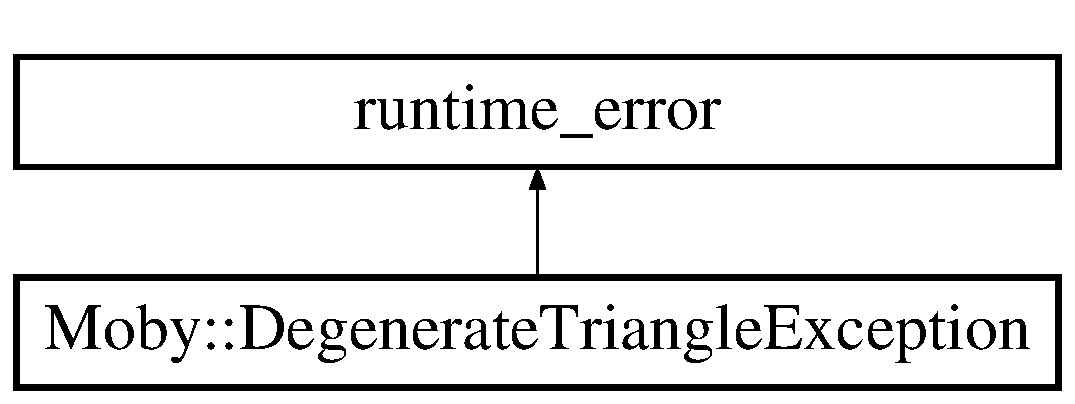
\includegraphics[height=2.000000cm]{classMoby_1_1DegenerateTriangleException}
\end{center}
\end{figure}


\subsection{Detailed Description}
Exception thrown when trying to perform an operation that requires a normal on a degenerate triangle. 

The documentation for this class was generated from the following file\-:\begin{DoxyCompactItemize}
\item 
/home/drum/\-Moby/include/\-Moby/Degenerate\-Triangle\-Exception.\-h\end{DoxyCompactItemize}

\section{Moby\-:\-:Dissipation Class Reference}
\label{classMoby_1_1Dissipation}\index{Moby\-::\-Dissipation@{Moby\-::\-Dissipation}}
Inheritance diagram for Moby\-:\-:Dissipation\-:\begin{figure}[H]
\begin{center}
\leavevmode
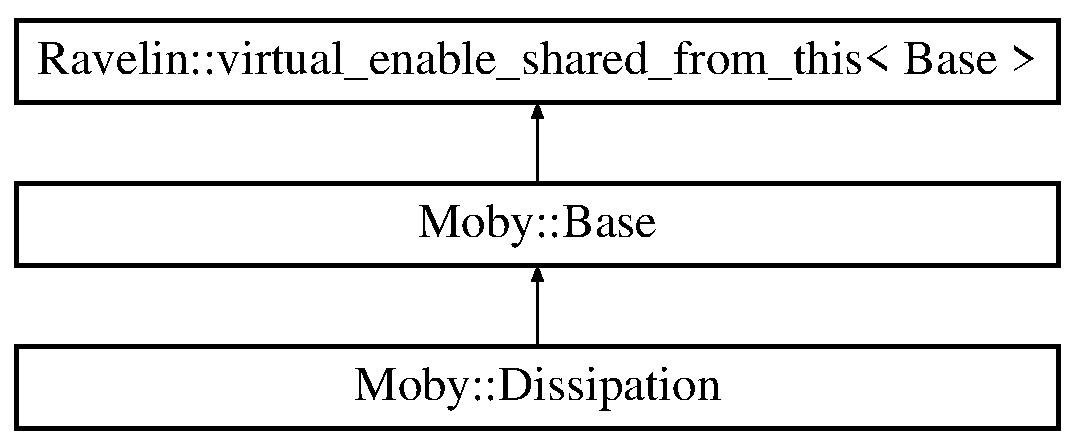
\includegraphics[height=3.000000cm]{classMoby_1_1Dissipation}
\end{center}
\end{figure}
\subsection*{Public Member Functions}
\begin{DoxyCompactItemize}
\item 
void {\bfseries apply} (const std\-::vector$<$ boost\-::shared\-\_\-ptr$<$ Ravelin\-::\-Dynamic\-Bodyd $>$ $>$ \&bodies)\label{classMoby_1_1Dissipation_aa4dc0baa81d59deeb50a71ebcce66599}

\item 
virtual void {\bf load\-\_\-from\-\_\-xml} (boost\-::shared\-\_\-ptr$<$ const {\bf X\-M\-L\-Tree} $>$ node, std\-::map$<$ std\-::string, {\bf Base\-Ptr} $>$ \&id\-\_\-map)\label{classMoby_1_1Dissipation_ac029254a743326952f34aa8ce21b1477}

\begin{DoxyCompactList}\small\item\em Implements \doxyref{Base\-::load\-\_\-from\-\_\-xml()}{p.}{classMoby_1_1Base_a98b861c1d615a748b576aa613f17389f} \end{DoxyCompactList}\item 
virtual void {\bf save\-\_\-to\-\_\-xml} ({\bf X\-M\-L\-Tree\-Ptr} node, std\-::list$<$ boost\-::shared\-\_\-ptr$<$ const {\bf Base} $>$ $>$ \&shared\-\_\-objects) const \label{classMoby_1_1Dissipation_ad064eff747616a8cd13d6385c49f4ff7}

\begin{DoxyCompactList}\small\item\em Implements \doxyref{Base\-::save\-\_\-to\-\_\-xml()}{p.}{classMoby_1_1Base_aed64905ca39893d02d1e6c3f03f73aa9} \end{DoxyCompactList}\end{DoxyCompactItemize}
\subsection*{Public Attributes}
\begin{DoxyCompactItemize}
\item 
std\-::map$<$ boost\-::shared\-\_\-ptr\\*
$<$ Ravelin\-::\-Dynamic\-Bodyd $>$\\*
, double $>$ {\bf \-\_\-coeffs}\label{classMoby_1_1Dissipation_aecfc659294f47db578702e60ad8c9d62}

\begin{DoxyCompactList}\small\item\em The mapping from bodies to decay coefficients. \end{DoxyCompactList}\end{DoxyCompactItemize}
\subsection*{Additional Inherited Members}


The documentation for this class was generated from the following files\-:\begin{DoxyCompactItemize}
\item 
/home/drum/\-Moby/include/\-Moby/Dissipation.\-h\item 
/home/drum/\-Moby/src/Dissipation.\-cpp\end{DoxyCompactItemize}

\section{Moby\-:\-:Dummy\-B\-V Class Reference}
\label{classMoby_1_1DummyBV}\index{Moby\-::\-Dummy\-B\-V@{Moby\-::\-Dummy\-B\-V}}


An abstract bounding volume.  




{\ttfamily \#include $<$Dummy\-B\-V.\-h$>$}

Inheritance diagram for Moby\-:\-:Dummy\-B\-V\-:\begin{figure}[H]
\begin{center}
\leavevmode
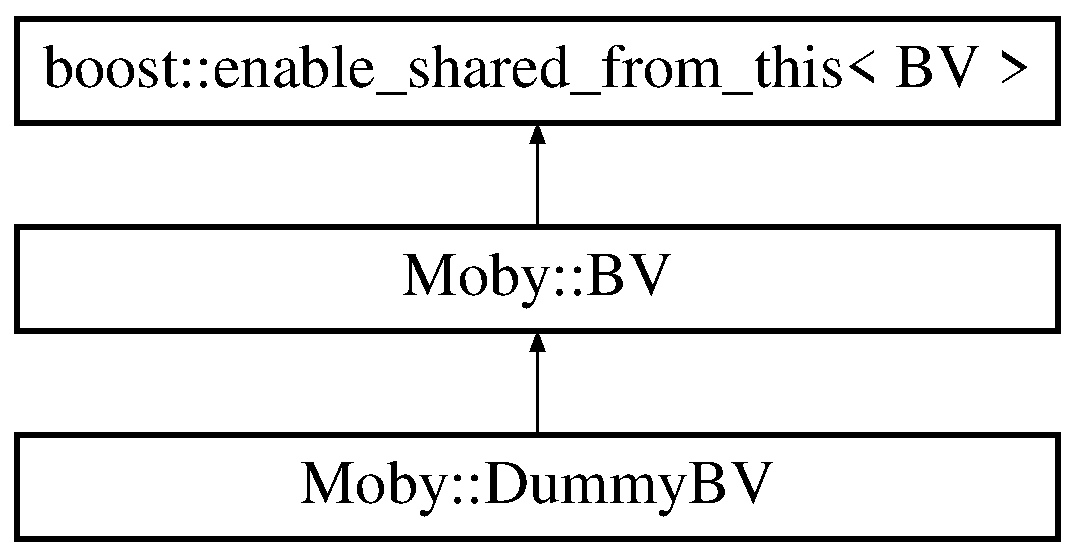
\includegraphics[height=3.000000cm]{classMoby_1_1DummyBV}
\end{center}
\end{figure}
\subsection*{Public Member Functions}
\begin{DoxyCompactItemize}
\item 
std\-::ostream \& {\bf to\-\_\-vrml} (std\-::ostream \&out, const Ravelin\-::\-Pose3d \&T) const \label{classMoby_1_1DummyBV_aed1c7debf70d6ea5d0409f62b8f76138}

\begin{DoxyCompactList}\small\item\em Nothing will be output. \end{DoxyCompactList}\item 
virtual boost\-::shared\-\_\-ptr\\*
$<$ const Ravelin\-::\-Pose3d $>$ {\bf get\-\_\-relative\-\_\-pose} () const \label{classMoby_1_1DummyBV_a1b058556ddb6bf278e4cbfba5f65d94e}

\begin{DoxyCompactList}\small\item\em Gets the associated pose for this bounding volume. \end{DoxyCompactList}\item 
virtual bool {\bf outside} (const {\bf Point3d} \&point, double tol=N\-E\-A\-R\-\_\-\-Z\-E\-R\-O) const \label{classMoby_1_1DummyBV_a8dbed5c75418e7ade58f1c05bcd0e642}

\begin{DoxyCompactList}\small\item\em Determines whether a point is outside the bounding volume. \end{DoxyCompactList}\item 
virtual bool {\bf intersects} (const {\bf Line\-Seg3} \&seg, double \&tmin, double tmax, {\bf Point3d} \&q) const \label{classMoby_1_1DummyBV_ad0b1338078a440a912d7293349f2d9af}

\begin{DoxyCompactList}\small\item\em Determines whether a line segment intersects the bounding volume. \end{DoxyCompactList}\item 
virtual {\bf B\-V\-Ptr} {\bf calc\-\_\-swept\-\_\-\-B\-V} ({\bf Collision\-Geometry\-Ptr} g, const Ravelin\-::\-S\-Velocityd \&v) const 
\begin{DoxyCompactList}\small\item\em Virtual function that calculates a velocity-\/expanded \doxyref{B\-V}{p.}{classMoby_1_1BV}. \end{DoxyCompactList}\item 
virtual double {\bf calc\-\_\-volume} () const \label{classMoby_1_1DummyBV_a0dec635421190be5ad8659bef388a5c4}

\begin{DoxyCompactList}\small\item\em Volume will be zero. \end{DoxyCompactList}\item 
virtual {\bf Point3d} {\bf get\-\_\-lower\-\_\-bounds} () const \label{classMoby_1_1DummyBV_afbe95bd0b88c3172bc85d8b7b11d0729}

\begin{DoxyCompactList}\small\item\em Gets the lower bounds. \end{DoxyCompactList}\item 
virtual {\bf Point3d} {\bf get\-\_\-upper\-\_\-bounds} () const \label{classMoby_1_1DummyBV_ac0a9e6fb85f42791eca7b1537fcd6f1c}

\begin{DoxyCompactList}\small\item\em Gets the upper bounds. \end{DoxyCompactList}\item 
virtual void {\bf transform} (const Ravelin\-::\-Transform3d \&T, {\bf B\-V} $\ast$result) const \label{classMoby_1_1DummyBV_a4b23e7d6e308ef3c1a857e3d6d8f1047}

\begin{DoxyCompactList}\small\item\em Transforms the dummy \doxyref{B\-V}{p.}{classMoby_1_1BV} (does nothing) \end{DoxyCompactList}\end{DoxyCompactItemize}
\subsection*{Additional Inherited Members}


\subsection{Detailed Description}
An abstract bounding volume. 

\begin{DoxyNote}{Note}
the \doxyref{B\-V}{p.}{classMoby_1_1BV} is generally constructed such that its frame is aligned with that of the underlying rigid body (or collision geometry). Therefore, the center of the \doxyref{B\-V}{p.}{classMoby_1_1BV} is computed relative to the center-\/of-\/mass of the body (or the center of the geometry). The orientation of the \doxyref{B\-V}{p.}{classMoby_1_1BV} will always be identical to the orientation of the rigid body (or collision geometry). 
\end{DoxyNote}


\subsection{Member Function Documentation}
\index{Moby\-::\-Dummy\-B\-V@{Moby\-::\-Dummy\-B\-V}!calc\-\_\-swept\-\_\-\-B\-V@{calc\-\_\-swept\-\_\-\-B\-V}}
\index{calc\-\_\-swept\-\_\-\-B\-V@{calc\-\_\-swept\-\_\-\-B\-V}!Moby::DummyBV@{Moby\-::\-Dummy\-B\-V}}
\subsubsection[{calc\-\_\-swept\-\_\-\-B\-V}]{\setlength{\rightskip}{0pt plus 5cm}virtual {\bf B\-V\-Ptr} Moby\-::\-Dummy\-B\-V\-::calc\-\_\-swept\-\_\-\-B\-V (
\begin{DoxyParamCaption}
\item[{{\bf Collision\-Geometry\-Ptr}}]{g, }
\item[{const Ravelin\-::\-S\-Velocityd \&}]{v}
\end{DoxyParamCaption}
) const\hspace{0.3cm}{\ttfamily [inline]}, {\ttfamily [virtual]}}\label{classMoby_1_1DummyBV_a025ef57dac043eb93f23f250e3817b7a}


Virtual function that calculates a velocity-\/expanded \doxyref{B\-V}{p.}{classMoby_1_1BV}. 


\begin{DoxyParams}{Parameters}
{\em g} & the geometry that this bounding volume represents \\
\hline
{\em dt} & the time step \\
\hline
{\em v} & the velocity \\
\hline
\end{DoxyParams}
\begin{DoxyReturn}{Returns}
the velocity-\/expanded bounding volume 
\end{DoxyReturn}


Implements {\bf Moby\-::\-B\-V} \doxyref{}{p.}{classMoby_1_1BV_a6aeddf29519a8d71d7318ca406d84582}.



The documentation for this class was generated from the following file\-:\begin{DoxyCompactItemize}
\item 
/home/drum/\-Moby/include/\-Moby/Dummy\-B\-V.\-h\end{DoxyCompactItemize}

\section{Moby\-:\-:Polyhedron\-:\-:Edge Struct Reference}
\label{structMoby_1_1Polyhedron_1_1Edge}\index{Moby\-::\-Polyhedron\-::\-Edge@{Moby\-::\-Polyhedron\-::\-Edge}}


The edge structure.  




{\ttfamily \#include $<$Polyhedron.\-h$>$}

Inheritance diagram for Moby\-:\-:Polyhedron\-:\-:Edge\-:\begin{figure}[H]
\begin{center}
\leavevmode
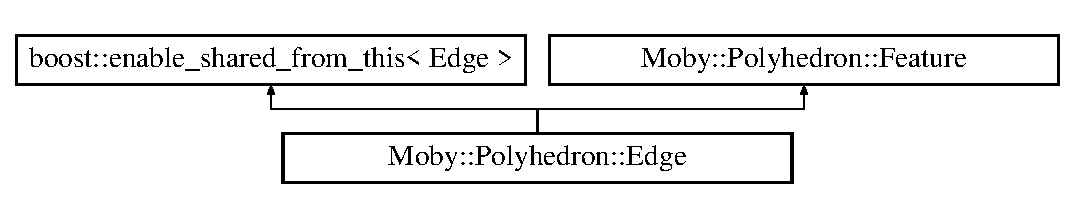
\includegraphics[height=2.000000cm]{structMoby_1_1Polyhedron_1_1Edge}
\end{center}
\end{figure}
\subsection*{Public Attributes}
\begin{DoxyCompactItemize}
\item 
boost\-::shared\-\_\-ptr$<$ {\bf Vertex} $>$ {\bfseries v1}\label{structMoby_1_1Polyhedron_1_1Edge_a51e7bc295faf3f0decef901b7201038b}

\item 
boost\-::shared\-\_\-ptr$<$ {\bf Vertex} $>$ {\bfseries v2}\label{structMoby_1_1Polyhedron_1_1Edge_a118efdc449f8593fcd0a9f4798cdd91f}

\item 
boost\-::shared\-\_\-ptr$<$ {\bf Face} $>$ {\bfseries face1}\label{structMoby_1_1Polyhedron_1_1Edge_a7497c2539606c6b2e26d493ab25ba257}

\item 
boost\-::shared\-\_\-ptr$<$ {\bf Face} $>$ {\bfseries face2}\label{structMoby_1_1Polyhedron_1_1Edge_abf5c19d33d76538d88f7fd2e982ec09d}

\item 
boost\-::shared\-\_\-ptr$<$ void $>$ {\bfseries data}\label{structMoby_1_1Polyhedron_1_1Edge_a068885f4e279d98161db5d7dc5cda343}

\end{DoxyCompactItemize}


\subsection{Detailed Description}
The edge structure. 

The documentation for this struct was generated from the following file\-:\begin{DoxyCompactItemize}
\item 
/home/drum/\-Moby/include/\-Moby/Polyhedron.\-h\end{DoxyCompactItemize}

\section{Moby\-:\-:Polyhedron\-:\-:Face Struct Reference}
\label{structMoby_1_1Polyhedron_1_1Face}\index{Moby\-::\-Polyhedron\-::\-Face@{Moby\-::\-Polyhedron\-::\-Face}}


The face structure.  




{\ttfamily \#include $<$Polyhedron.\-h$>$}

Inheritance diagram for Moby\-:\-:Polyhedron\-:\-:Face\-:\begin{figure}[H]
\begin{center}
\leavevmode
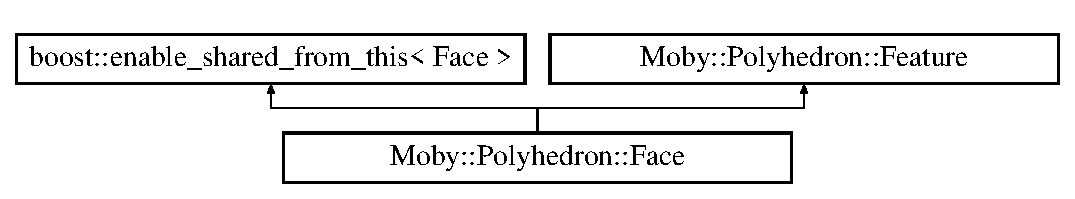
\includegraphics[height=2.000000cm]{structMoby_1_1Polyhedron_1_1Face}
\end{center}
\end{figure}
\subsection*{Public Member Functions}
\begin{DoxyCompactItemize}
\item 
{\bf Plane} {\bf get\-\_\-plane} () const \label{structMoby_1_1Polyhedron_1_1Face_a7974184821525910e93b0a4b1a8ad997}

\begin{DoxyCompactList}\small\item\em Gets the plane containing a face. \end{DoxyCompactList}\end{DoxyCompactItemize}
\subsection*{Public Attributes}
\begin{DoxyCompactItemize}
\item 
std\-::list$<$ boost\-::weak\-\_\-ptr\\*
$<$ {\bf Edge} $>$ $>$ {\bfseries e}\label{structMoby_1_1Polyhedron_1_1Face_a2abe4b7edeab1e97b77fd5026971bbd9}

\item 
boost\-::shared\-\_\-ptr$<$ void $>$ {\bfseries data}\label{structMoby_1_1Polyhedron_1_1Face_abbbcf82287e4200c6dc2ab114cb70cde}

\end{DoxyCompactItemize}


\subsection{Detailed Description}
The face structure. 

The documentation for this struct was generated from the following files\-:\begin{DoxyCompactItemize}
\item 
/home/drum/\-Moby/include/\-Moby/Polyhedron.\-h\item 
/home/drum/\-Moby/src/Polyhedron.\-cpp\end{DoxyCompactItemize}

\section{Moby\-:\-:Polyhedron\-:\-:Feature Struct Reference}
\label{structMoby_1_1Polyhedron_1_1Feature}\index{Moby\-::\-Polyhedron\-::\-Feature@{Moby\-::\-Polyhedron\-::\-Feature}}


A vertex, face, or edge in a polyhedron.  




{\ttfamily \#include $<$Polyhedron.\-h$>$}

Inheritance diagram for Moby\-:\-:Polyhedron\-:\-:Feature\-:\begin{figure}[H]
\begin{center}
\leavevmode
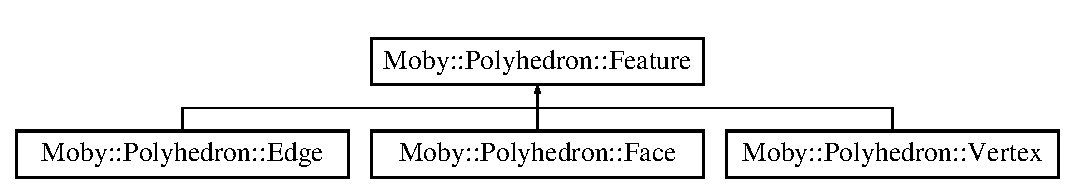
\includegraphics[height=2.000000cm]{structMoby_1_1Polyhedron_1_1Feature}
\end{center}
\end{figure}


\subsection{Detailed Description}
A vertex, face, or edge in a polyhedron. 

The documentation for this struct was generated from the following file\-:\begin{DoxyCompactItemize}
\item 
/home/drum/\-Moby/include/\-Moby/Polyhedron.\-h\end{DoxyCompactItemize}

\section{Moby\-:\-:Fixed\-Joint Class Reference}
\label{classMoby_1_1FixedJoint}\index{Moby\-::\-Fixed\-Joint@{Moby\-::\-Fixed\-Joint}}


Defines a joint for fixing two bodies together or fixing one body to the ground.  




{\ttfamily \#include $<$Fixed\-Joint.\-h$>$}

Inheritance diagram for Moby\-:\-:Fixed\-Joint\-:\begin{figure}[H]
\begin{center}
\leavevmode
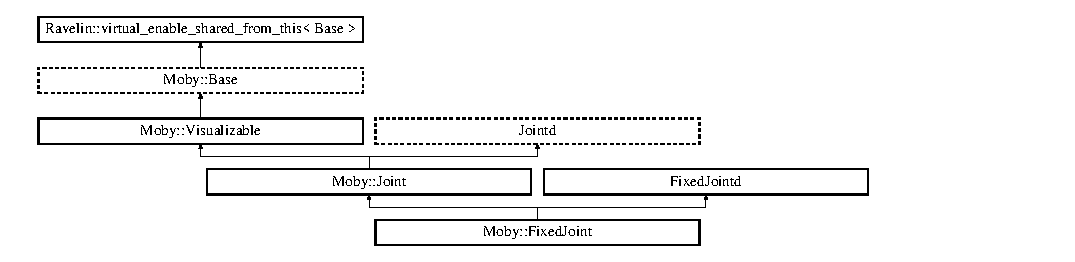
\includegraphics[height=3.070176cm]{classMoby_1_1FixedJoint}
\end{center}
\end{figure}
\subsection*{Public Member Functions}
\begin{DoxyCompactItemize}
\item 
{\bf Fixed\-Joint} ()
\begin{DoxyCompactList}\small\item\em Initializes the joint. \end{DoxyCompactList}\item 
{\bf Fixed\-Joint} (boost\-::weak\-\_\-ptr$<$ {\bf Rigid\-Body} $>$ inboard, boost\-::weak\-\_\-ptr$<$ {\bf Rigid\-Body} $>$ outboard)\label{classMoby_1_1FixedJoint_aa08bb6cd8972ebc448a05a810608fba0}

\begin{DoxyCompactList}\small\item\em Initializes the joint with the specified inboard and outboard links. \end{DoxyCompactList}\item 
virtual unsigned {\bfseries num\-\_\-dof} () const \label{classMoby_1_1FixedJoint_a1c7512ec1d003ca7b67450a479bfc6e8}

\item 
virtual bool {\bfseries is\-\_\-singular\-\_\-config} () const \label{classMoby_1_1FixedJoint_aaa0f02261e54e3c1a40f1bb4ebef5a28}

\item 
virtual void {\bfseries evaluate\-\_\-constraints} (double C[$\,$])\label{classMoby_1_1FixedJoint_aba72f09b9e9bba18d2bbd0a0ba269baf}

\item 
virtual const std\-::vector\\*
$<$ Ravelin\-::\-S\-Velocityd $>$ \& {\bfseries get\-\_\-spatial\-\_\-axes\-\_\-dot} ()\label{classMoby_1_1FixedJoint_a84c5b8f1c91c1f744703209c76c5e225}

\item 
virtual void {\bfseries determine\-\_\-q} (Ravelin\-::\-Vector\-Nd \&q)\label{classMoby_1_1FixedJoint_a63d5ed33ab218c68558ac543d7879db5}

\item 
virtual boost\-::shared\-\_\-ptr\\*
$<$ const Ravelin\-::\-Pose3d $>$ {\bfseries get\-\_\-induced\-\_\-pose} ()\label{classMoby_1_1FixedJoint_ae6cf80897ad8a62deefb8211cfe6eb11}

\item 
virtual void {\bf load\-\_\-from\-\_\-xml} (boost\-::shared\-\_\-ptr$<$ const {\bf X\-M\-L\-Tree} $>$ node, std\-::map$<$ std\-::string, {\bf Base\-Ptr} $>$ \&id\-\_\-map)\label{classMoby_1_1FixedJoint_a02e637422d026f869ab138b3c76de654}

\begin{DoxyCompactList}\small\item\em Implements \doxyref{Base\-::load\-\_\-from\-\_\-xml()}{p.}{classMoby_1_1Base_a98b861c1d615a748b576aa613f17389f} \end{DoxyCompactList}\item 
virtual void {\bf save\-\_\-to\-\_\-xml} ({\bf X\-M\-L\-Tree\-Ptr} node, std\-::list$<$ boost\-::shared\-\_\-ptr$<$ const {\bf Base} $>$ $>$ \&shared\-\_\-objects) const \label{classMoby_1_1FixedJoint_abd170c47b08339efdc26ea5929aea3a3}

\begin{DoxyCompactList}\small\item\em Implements \doxyref{Base\-::save\-\_\-to\-\_\-xml()}{p.}{classMoby_1_1Base_aed64905ca39893d02d1e6c3f03f73aa9} \end{DoxyCompactList}\end{DoxyCompactItemize}
\subsection*{Additional Inherited Members}


\subsection{Detailed Description}
Defines a joint for fixing two bodies together or fixing one body to the ground. 

\subsection{Constructor \& Destructor Documentation}
\index{Moby\-::\-Fixed\-Joint@{Moby\-::\-Fixed\-Joint}!Fixed\-Joint@{Fixed\-Joint}}
\index{Fixed\-Joint@{Fixed\-Joint}!Moby::FixedJoint@{Moby\-::\-Fixed\-Joint}}
\subsubsection[{Fixed\-Joint}]{\setlength{\rightskip}{0pt plus 5cm}Fixed\-Joint\-::\-Fixed\-Joint (
\begin{DoxyParamCaption}
{}
\end{DoxyParamCaption}
)}\label{classMoby_1_1FixedJoint_ab66790cd6e3b1ffb7f6c0acfc7c11540}


Initializes the joint. 

The inboard and outboard links are set to N\-U\-L\-L. 

References Moby\-::\-Joint\-::init\-\_\-data().



The documentation for this class was generated from the following files\-:\begin{DoxyCompactItemize}
\item 
/home/drum/\-Moby/include/\-Moby/Fixed\-Joint.\-h\item 
/home/drum/\-Moby/src/Fixed\-Joint.\-cpp\end{DoxyCompactItemize}

\section{Moby\-:\-:Gears Class Reference}
\label{classMoby_1_1Gears}\index{Moby\-::\-Gears@{Moby\-::\-Gears}}


Defines a gear (\char`\"{}joint\char`\"{}) constraint.  




{\ttfamily \#include $<$Gears.\-h$>$}

Inheritance diagram for Moby\-:\-:Gears\-:\begin{figure}[H]
\begin{center}
\leavevmode
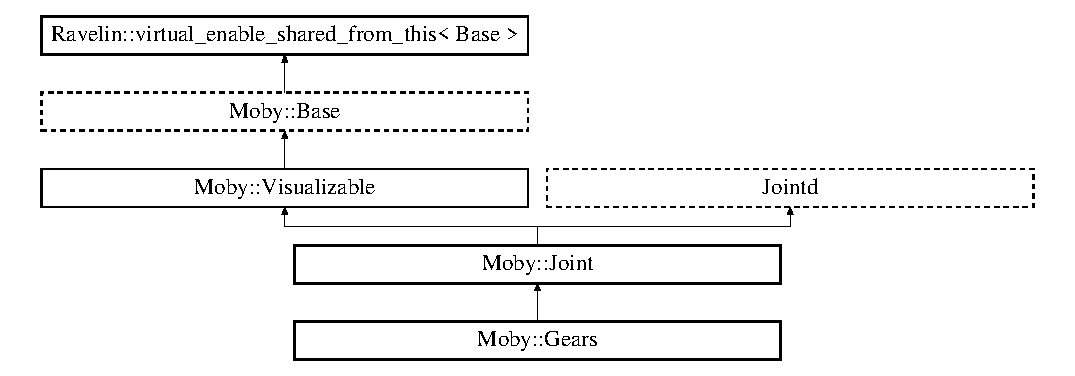
\includegraphics[height=4.605263cm]{classMoby_1_1Gears}
\end{center}
\end{figure}
\subsection*{Public Member Functions}
\begin{DoxyCompactItemize}
\item 
{\bf Gears} ()
\begin{DoxyCompactList}\small\item\em Initializes the joint. \end{DoxyCompactList}\item 
virtual void {\bf save\-\_\-to\-\_\-xml} ({\bf X\-M\-L\-Tree\-Ptr} node, std\-::list$<$ boost\-::shared\-\_\-ptr$<$ const {\bf Base} $>$ $>$ \&shared\-\_\-objects) const \label{classMoby_1_1Gears_a9aa0d3984cc06b49b42bccfe6e86f4dd}

\begin{DoxyCompactList}\small\item\em Implements \doxyref{Base\-::save\-\_\-to\-\_\-xml()}{p.}{classMoby_1_1Base_aed64905ca39893d02d1e6c3f03f73aa9} \end{DoxyCompactList}\item 
virtual void {\bf load\-\_\-from\-\_\-xml} (boost\-::shared\-\_\-ptr$<$ const {\bf X\-M\-L\-Tree} $>$ node, std\-::map$<$ std\-::string, {\bf Base\-Ptr} $>$ \&id\-\_\-map)\label{classMoby_1_1Gears_a5e7fe5c59b73c07c727715640f067dfb}

\begin{DoxyCompactList}\small\item\em Implements \doxyref{Base\-::load\-\_\-from\-\_\-xml()}{p.}{classMoby_1_1Base_a98b861c1d615a748b576aa613f17389f} \end{DoxyCompactList}\item 
virtual void {\bf set\-\_\-inboard\-\_\-pose} (boost\-::shared\-\_\-ptr$<$ const Ravelin\-::\-Pose3d $>$ link, bool update\-\_\-joint\-\_\-pose)\label{classMoby_1_1Gears_ab673b810869c2c8296a86ea15041dbf9}

\begin{DoxyCompactList}\small\item\em Sets the inboard pose. \end{DoxyCompactList}\item 
virtual void {\bf set\-\_\-outboard\-\_\-pose} (boost\-::shared\-\_\-ptr$<$ const Ravelin\-::\-Pose3d $>$ link, bool update\-\_\-joint\-\_\-pose)\label{classMoby_1_1Gears_a4a41bb274fb365d075c907ccbbe7ec50}

\begin{DoxyCompactList}\small\item\em Sets the outboard pose. \end{DoxyCompactList}\item 
virtual void {\bf evaluate\-\_\-constraints} (double C[$\,$])\label{classMoby_1_1Gears_aa9c22bfad46e318c6b0e68eae324053b}

\begin{DoxyCompactList}\small\item\em Evaluates the joint constraint. \end{DoxyCompactList}\item 
virtual void {\bf evaluate\-\_\-constraints\-\_\-dot} (double C[$\,$])\label{classMoby_1_1Gears_a3c88626935ff7a6e7a256a4782d1fa6f}

\begin{DoxyCompactList}\small\item\em Evaluates the time derivative of the constraint. \end{DoxyCompactList}\item 
virtual void {\bf calc\-\_\-constraint\-\_\-jacobian} (bool inboard, Ravelin\-::\-Matrix\-Nd \&Cq)\label{classMoby_1_1Gears_a461175e8767bb8f37287a74ab644e246}

\begin{DoxyCompactList}\small\item\em Computes the constraint Jacobian. \end{DoxyCompactList}\item 
virtual void {\bf calc\-\_\-constraint\-\_\-jacobian\-\_\-dot} (bool inboard, Ravelin\-::\-Matrix\-Nd \&Cq)\label{classMoby_1_1Gears_af1bcda49a7f953ece9f2a33a44ab050a}

\begin{DoxyCompactList}\small\item\em Computes the time derivative of the constraint Jacobian. \end{DoxyCompactList}\item 
virtual unsigned {\bfseries num\-\_\-dof} () const \label{classMoby_1_1Gears_ac01b65eb0c1c8235c94627716986fdd3}

\item 
virtual unsigned {\bfseries num\-\_\-constraint\-\_\-eqns} () const \label{classMoby_1_1Gears_a98c857db3631cb409b1d8530815b859a}

\item 
virtual void {\bfseries determine\-\_\-q} (Ravelin\-::\-Vector\-Nd \&q)\label{classMoby_1_1Gears_a4618fff2d728ecb532633ae8ceeb41c2}

\item 
virtual boost\-::shared\-\_\-ptr\\*
$<$ const Ravelin\-::\-Pose3d $>$ {\bfseries get\-\_\-induced\-\_\-pose} ()\label{classMoby_1_1Gears_a6a02d45cff9423c8060eda79bd4ef228}

\item 
virtual bool {\bfseries is\-\_\-singular\-\_\-config} () const \label{classMoby_1_1Gears_a40b04603fde0c395b93d6ccbe5bc1fae}

\item 
virtual const std\-::vector\\*
$<$ Ravelin\-::\-S\-Velocityd $>$ \& {\bfseries get\-\_\-spatial\-\_\-axes\-\_\-dot} ()\label{classMoby_1_1Gears_ab31482493b1883df6940991877e34f25}

\end{DoxyCompactItemize}
\subsection*{Additional Inherited Members}


\subsection{Detailed Description}
Defines a gear (\char`\"{}joint\char`\"{}) constraint. 

\begin{DoxyRefDesc}{Todo}
\item[{\bf Todo}]implement a rest position for q? \end{DoxyRefDesc}


\subsection{Constructor \& Destructor Documentation}
\index{Moby\-::\-Gears@{Moby\-::\-Gears}!Gears@{Gears}}
\index{Gears@{Gears}!Moby::Gears@{Moby\-::\-Gears}}
\subsubsection[{Gears}]{\setlength{\rightskip}{0pt plus 5cm}Gears\-::\-Gears (
\begin{DoxyParamCaption}
{}
\end{DoxyParamCaption}
)}\label{classMoby_1_1Gears_a53cdddb207f56ccddc9219b42e938724}


Initializes the joint. 

The gear ratio is set to 1\-:1 

References Moby\-::\-Joint\-::init\-\_\-data().



The documentation for this class was generated from the following files\-:\begin{DoxyCompactItemize}
\item 
/home/drum/\-Moby/include/\-Moby/Gears.\-h\item 
/home/drum/\-Moby/src/Gears.\-cpp\end{DoxyCompactItemize}

\section{Moby\-:\-:Gravity\-Force Class Reference}
\label{classMoby_1_1GravityForce}\index{Moby\-::\-Gravity\-Force@{Moby\-::\-Gravity\-Force}}


Gravitational force applied to bodies.  




{\ttfamily \#include $<$Gravity\-Force.\-h$>$}

Inheritance diagram for Moby\-:\-:Gravity\-Force\-:\begin{figure}[H]
\begin{center}
\leavevmode
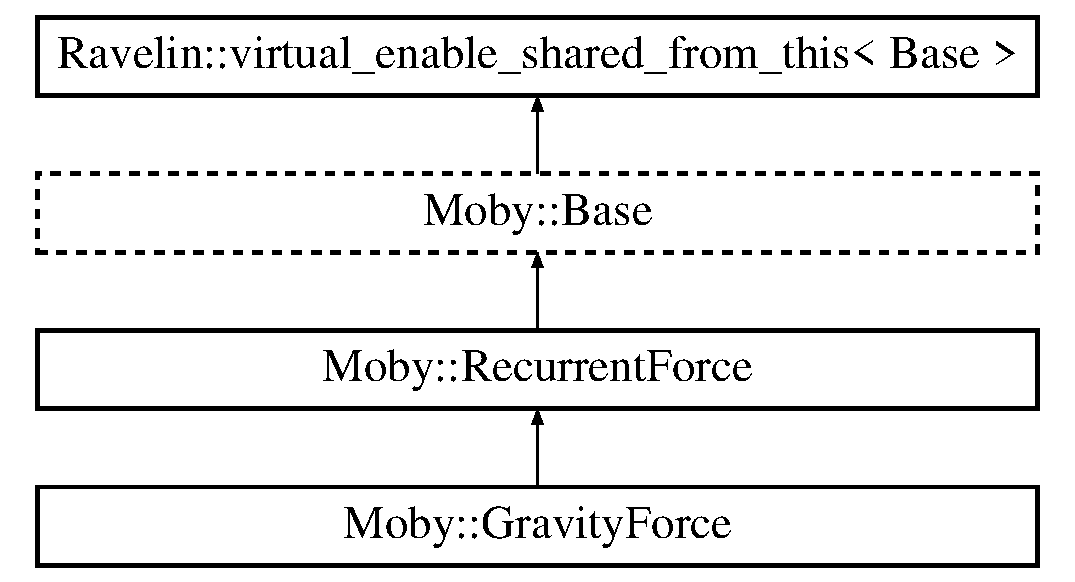
\includegraphics[height=4.000000cm]{classMoby_1_1GravityForce}
\end{center}
\end{figure}
\subsection*{Public Member Functions}
\begin{DoxyCompactItemize}
\item 
{\bf Gravity\-Force} ()\label{classMoby_1_1GravityForce_aeb50d78dec81457555581e491e5a998f}

\begin{DoxyCompactList}\small\item\em Constructs a default gravity vector of [0,0,0]. \end{DoxyCompactList}\item 
{\bf Gravity\-Force} (const {\bf Gravity\-Force} \&source)\label{classMoby_1_1GravityForce_aaafe476d1b53bc0c0099fefd89b475ac}

\begin{DoxyCompactList}\small\item\em Copy constructor. \end{DoxyCompactList}\item 
virtual void {\bf add\-\_\-force} (boost\-::shared\-\_\-ptr$<$ Ravelin\-::\-Dynamic\-Bodyd $>$ body)\label{classMoby_1_1GravityForce_acffa01fe90179839d76a7d695bf8e057}

\begin{DoxyCompactList}\small\item\em Adds gravity to a body. \end{DoxyCompactList}\item 
virtual void {\bf load\-\_\-from\-\_\-xml} (boost\-::shared\-\_\-ptr$<$ const {\bf X\-M\-L\-Tree} $>$ node, std\-::map$<$ std\-::string, {\bf Base\-Ptr} $>$ \&id\-\_\-map)\label{classMoby_1_1GravityForce_a61d8468de9c5bc8d2a8853bec08d14fe}

\begin{DoxyCompactList}\small\item\em Implements \doxyref{Base\-::load\-\_\-from\-\_\-xml()}{p.}{classMoby_1_1Base_a98b861c1d615a748b576aa613f17389f} \end{DoxyCompactList}\item 
virtual void {\bf save\-\_\-to\-\_\-xml} ({\bf X\-M\-L\-Tree\-Ptr} node, std\-::list$<$ boost\-::shared\-\_\-ptr$<$ const {\bf Base} $>$ $>$ \&shared\-\_\-objects) const \label{classMoby_1_1GravityForce_af3d2dc707d49572209c0b24105cecc98}

\begin{DoxyCompactList}\small\item\em Implements \doxyref{Base\-::save\-\_\-to\-\_\-xml()}{p.}{classMoby_1_1Base_aed64905ca39893d02d1e6c3f03f73aa9} \end{DoxyCompactList}\end{DoxyCompactItemize}
\subsection*{Public Attributes}
\begin{DoxyCompactItemize}
\item 
Ravelin\-::\-Vector3d {\bf gravity}\label{classMoby_1_1GravityForce_af8edac4814fd8597ed769b945d71e9c5}

\begin{DoxyCompactList}\small\item\em The gravity vector. \end{DoxyCompactList}\end{DoxyCompactItemize}
\subsection*{Additional Inherited Members}


\subsection{Detailed Description}
Gravitational force applied to bodies. 

The documentation for this class was generated from the following files\-:\begin{DoxyCompactItemize}
\item 
/home/drum/\-Moby/include/\-Moby/Gravity\-Force.\-h\item 
/home/drum/\-Moby/src/Gravity\-Force.\-cpp\end{DoxyCompactItemize}

\section{Moby\-:\-:Heightmap\-Primitive Class Reference}
\label{classMoby_1_1HeightmapPrimitive}\index{Moby\-::\-Heightmap\-Primitive@{Moby\-::\-Heightmap\-Primitive}}


Represents a heightmap with height zero on the xz plane (primitive can be transformed)  




{\ttfamily \#include $<$Heightmap\-Primitive.\-h$>$}

Inheritance diagram for Moby\-:\-:Heightmap\-Primitive\-:\begin{figure}[H]
\begin{center}
\leavevmode
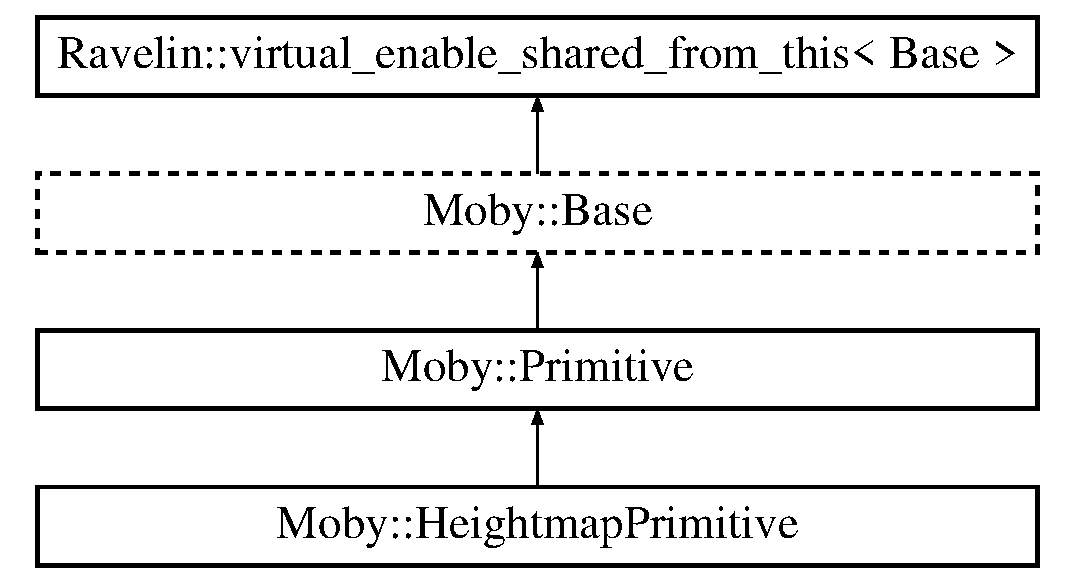
\includegraphics[height=4.000000cm]{classMoby_1_1HeightmapPrimitive}
\end{center}
\end{figure}
\subsection*{Public Member Functions}
\begin{DoxyCompactItemize}
\item 
{\bf Heightmap\-Primitive} ()\label{classMoby_1_1HeightmapPrimitive_aba9f39660ed89b83f7b0391b86e3cc6f}

\begin{DoxyCompactList}\small\item\em Initializes the heightmap primitive. \end{DoxyCompactList}\item 
{\bf Heightmap\-Primitive} (const Ravelin\-::\-Pose3d \&T)\label{classMoby_1_1HeightmapPrimitive_a4e2f7ce5a3ba1bf280d8e372e64c2aaa}

\begin{DoxyCompactList}\small\item\em Initializes the heightmap primitive. \end{DoxyCompactList}\item 
virtual void {\bf set\-\_\-pose} (const Ravelin\-::\-Pose3d \&T)\label{classMoby_1_1HeightmapPrimitive_ab5c28ce6a8384176f3c87e2323ced3c8}

\begin{DoxyCompactList}\small\item\em Transforms the primitive. \end{DoxyCompactList}\item 
virtual void {\bf get\-\_\-vertices} (boost\-::shared\-\_\-ptr$<$ const Ravelin\-::\-Pose3d $>$ P, std\-::vector$<$ {\bf Point3d} $>$ \&vertices) const 
\begin{DoxyCompactList}\small\item\em Get vertices corresponding to this primitive. \end{DoxyCompactList}\item 
void {\bfseries get\-\_\-vertices} ({\bf B\-V\-Ptr} bv, boost\-::shared\-\_\-ptr$<$ const Ravelin\-::\-Pose3d $>$ P, std\-::vector$<$ {\bf Point3d} $>$ \&vertices) const \label{classMoby_1_1HeightmapPrimitive_a88e6528562f1b8f1a91b24bfef2f4650}

\item 
virtual double {\bf calc\-\_\-dist\-\_\-and\-\_\-normal} (const {\bf Point3d} \&point, std\-::vector$<$ Ravelin\-::\-Vector3d $>$ \&normals) const \label{classMoby_1_1HeightmapPrimitive_a40b0fb0723fa1a9e0d5dec65dc70e439}

\begin{DoxyCompactList}\small\item\em Finds the signed distance betwen the heightmap and a point. \end{DoxyCompactList}\item 
virtual double {\bf calc\-\_\-signed\-\_\-dist} (boost\-::shared\-\_\-ptr$<$ const {\bf Primitive} $>$ p, {\bf Point3d} \&pthis, {\bf Point3d} \&pp) const \label{classMoby_1_1HeightmapPrimitive_add7ce488c84ecc7ab03b53e6118c09eb}

\begin{DoxyCompactList}\small\item\em Computes the signed distance between this and another primitive. \end{DoxyCompactList}\item 
double {\bfseries calc\-\_\-signed\-\_\-dist} (boost\-::shared\-\_\-ptr$<$ const {\bf Sphere\-Primitive} $>$ s, {\bf Point3d} \&pthis, {\bf Point3d} \&psph) const \label{classMoby_1_1HeightmapPrimitive_a5057dd025d37deaf8a0e538ee995ac85}

\item 
virtual {\bf Point3d} {\bf get\-\_\-supporting\-\_\-point} (const Ravelin\-::\-Vector3d \&d) const \label{classMoby_1_1HeightmapPrimitive_a0792ec0d3414b63d7439ca19fd47530f}

\begin{DoxyCompactList}\small\item\em Gets the supporting point. \end{DoxyCompactList}\item 
virtual double {\bf calc\-\_\-signed\-\_\-dist} (const {\bf Point3d} \&p) const \label{classMoby_1_1HeightmapPrimitive_a3289cff9c06234c2694b02eec010ac9d}

\begin{DoxyCompactList}\small\item\em Computes the signed distance of the given point from this primitive. \end{DoxyCompactList}\item 
virtual osg\-::\-Node $\ast$ {\bf create\-\_\-visualization} ()\label{classMoby_1_1HeightmapPrimitive_ad258b5f84a0c39fd04019e95ddb69288}

\begin{DoxyCompactList}\small\item\em Computes the O\-S\-G visualization. \end{DoxyCompactList}\item 
virtual boost\-::shared\-\_\-ptr\\*
$<$ const {\bf Indexed\-Tri\-Array} $>$ {\bf get\-\_\-mesh} (boost\-::shared\-\_\-ptr$<$ const Ravelin\-::\-Pose3d $>$ P)\label{classMoby_1_1HeightmapPrimitive_a86d2f9cef6c7c5333fa07c21e4edf9d3}

\begin{DoxyCompactList}\small\item\em Gets the mesh of the heightmap. \end{DoxyCompactList}\item 
virtual void {\bfseries calc\-\_\-mass\-\_\-properties} ()\label{classMoby_1_1HeightmapPrimitive_a20b855c6f3cc2e593370a4dcb6ba888f}

\item 
virtual {\bf B\-V\-Ptr} {\bf get\-\_\-\-B\-V\-H\-\_\-root} ({\bf Collision\-Geometry\-Ptr} geom)\label{classMoby_1_1HeightmapPrimitive_a7e715fc574ff7e8d64312a2960a03d47}

\begin{DoxyCompactList}\small\item\em Gets the B\-V\-H root for the heightmap. \end{DoxyCompactList}\item 
virtual void {\bf load\-\_\-from\-\_\-xml} (boost\-::shared\-\_\-ptr$<$ const {\bf X\-M\-L\-Tree} $>$ node, std\-::map$<$ std\-::string, {\bf Base\-Ptr} $>$ \&id\-\_\-map)\label{classMoby_1_1HeightmapPrimitive_acbe882c1a5fd97b2537a0cbab860e8a4}

\begin{DoxyCompactList}\small\item\em Implements \doxyref{Base\-::load\-\_\-from\-\_\-xml()}{p.}{classMoby_1_1Base_a98b861c1d615a748b576aa613f17389f} for serialization. \end{DoxyCompactList}\item 
virtual void {\bf save\-\_\-to\-\_\-xml} ({\bf X\-M\-L\-Tree\-Ptr} node, std\-::list$<$ boost\-::shared\-\_\-ptr$<$ const {\bf Base} $>$ $>$ \&shared\-\_\-objects) const \label{classMoby_1_1HeightmapPrimitive_a36f1a53d9a69a39f944ff1462ef161b6}

\begin{DoxyCompactList}\small\item\em Implements \doxyref{Base\-::save\-\_\-to\-\_\-xml()}{p.}{classMoby_1_1Base_aed64905ca39893d02d1e6c3f03f73aa9} for serialization. \end{DoxyCompactList}\item 
const Ravelin\-::\-Matrix\-Nd \& {\bfseries get\-\_\-heights} () const \label{classMoby_1_1HeightmapPrimitive_a6cdc4bca5c733fca04f071ff00d2c34f}

\item 
double {\bfseries get\-\_\-width} () const \label{classMoby_1_1HeightmapPrimitive_a63188bfef13a32c61269a65f56cc33dc}

\item 
double {\bfseries get\-\_\-depth} () const \label{classMoby_1_1HeightmapPrimitive_a41eb49505c6a9c7b3870ee3e094ec132}

\item 
virtual double {\bfseries get\-\_\-bounding\-\_\-radius} () const \label{classMoby_1_1HeightmapPrimitive_a5d2147f3b2b2f1508dcaecfed8e8b8f3}

\end{DoxyCompactItemize}
\subsection*{Protected Member Functions}
\begin{DoxyCompactItemize}
\item 
virtual double {\bf calc\-\_\-height} (const {\bf Point3d} \&p) const \label{classMoby_1_1HeightmapPrimitive_a1478f02eef432012d94eb30d3818ccbe}

\begin{DoxyCompactList}\small\item\em Computes the height at a particular point. \end{DoxyCompactList}\item 
void {\bf calc\-\_\-gradient} (const {\bf Point3d} \&p, double \&gx, double \&gz) const \label{classMoby_1_1HeightmapPrimitive_a7d8061c5f8269ba287cc7ecd555eb139}

\begin{DoxyCompactList}\small\item\em Computes the gradient at a particular point. \end{DoxyCompactList}\end{DoxyCompactItemize}
\subsection*{Protected Attributes}
\begin{DoxyCompactItemize}
\item 
double {\bf \-\_\-width}\label{classMoby_1_1HeightmapPrimitive_a976645f4a9374e20d0d639212881dc2b}

\begin{DoxyCompactList}\small\item\em width of the heightmap \end{DoxyCompactList}\item 
double {\bf \-\_\-depth}\label{classMoby_1_1HeightmapPrimitive_a2304ffcc7e1f8e2e0a966552a5a84cb7}

\begin{DoxyCompactList}\small\item\em depth of the heightmap \end{DoxyCompactList}\item 
Ravelin\-::\-Matrix\-Nd {\bfseries \-\_\-heights}\label{classMoby_1_1HeightmapPrimitive_af47bf202e8beb1fcd80f4f11e4291a26}

\item 
std\-::map$<$ {\bf Collision\-Geometry\-Ptr}, \\*
boost\-::shared\-\_\-ptr$<$ {\bf O\-B\-B} $>$ $>$ {\bf \-\_\-obbs}\label{classMoby_1_1HeightmapPrimitive_a1a99852b08ac58a3870868486da4e7fc}

\begin{DoxyCompactList}\small\item\em The bounding volumes for the heightmap. \end{DoxyCompactList}\end{DoxyCompactItemize}
\subsection*{Friends}
\begin{DoxyCompactItemize}
\item 
class {\bfseries C\-C\-D}\label{classMoby_1_1HeightmapPrimitive_aab79385077be6367d4557d44e17ffcf0}

\end{DoxyCompactItemize}
\subsection*{Additional Inherited Members}


\subsection{Detailed Description}
Represents a heightmap with height zero on the xz plane (primitive can be transformed) 

\subsection{Member Function Documentation}
\index{Moby\-::\-Heightmap\-Primitive@{Moby\-::\-Heightmap\-Primitive}!get\-\_\-vertices@{get\-\_\-vertices}}
\index{get\-\_\-vertices@{get\-\_\-vertices}!Moby::HeightmapPrimitive@{Moby\-::\-Heightmap\-Primitive}}
\subsubsection[{get\-\_\-vertices}]{\setlength{\rightskip}{0pt plus 5cm}virtual void Moby\-::\-Heightmap\-Primitive\-::get\-\_\-vertices (
\begin{DoxyParamCaption}
\item[{boost\-::shared\-\_\-ptr$<$ const Ravelin\-::\-Pose3d $>$}]{P, }
\item[{std\-::vector$<$ {\bf Point3d} $>$ \&}]{vertices}
\end{DoxyParamCaption}
) const\hspace{0.3cm}{\ttfamily [virtual]}}\label{classMoby_1_1HeightmapPrimitive_ae24de93fef445d0c3ed621fbd65465a1}


Get vertices corresponding to this primitive. 

Gets the vertex indices from selected facets of an \doxyref{Indexed\-Tri\-Array}{p.}{classMoby_1_1IndexedTriArray}.


\begin{DoxyParams}{Parameters}
{\em tris} & the triangle mesh \\
\hline
{\em fselect\-\_\-begin} & iterator to a container of type unsigned (facet indices) \\
\hline
{\em fselect\-\_\-end} & iterator to a container of type unsigned (facet indices) \\
\hline
{\em output} & beginning iterator to a container of type Point3d; unique vertices are copied here on return \\
\hline
\end{DoxyParams}
\begin{DoxyReturn}{Returns}
ending iterator to a container of type Point3d; unique vertices are copied here on return 
\end{DoxyReturn}


Implements {\bf Moby\-::\-Primitive} \doxyref{}{p.}{classMoby_1_1Primitive_ab50adaba8785794650193def668d4a05}.



Referenced by create\-\_\-visualization().



The documentation for this class was generated from the following files\-:\begin{DoxyCompactItemize}
\item 
/home/drum/\-Moby/include/\-Moby/Heightmap\-Primitive.\-h\item 
/home/drum/\-Moby/src/Heightmap\-Primitive.\-cpp\end{DoxyCompactItemize}

\section{Moby\-:\-:Impact\-Constraint\-Handler Class Reference}
\label{classMoby_1_1ImpactConstraintHandler}\index{Moby\-::\-Impact\-Constraint\-Handler@{Moby\-::\-Impact\-Constraint\-Handler}}


Defines the mechanism for handling impact constraints.  




{\ttfamily \#include $<$Impact\-Constraint\-Handler.\-h$>$}

\subsection*{Public Member Functions}
\begin{DoxyCompactItemize}
\item 
{\bf Impact\-Constraint\-Handler} ()\label{classMoby_1_1ImpactConstraintHandler_ac40db75508e330d0e3506f834b7309d3}

\begin{DoxyCompactList}\small\item\em Sets up the default parameters for the impact event handler. \end{DoxyCompactList}\item 
void {\bf process\-\_\-constraints} (const std\-::vector$<$ {\bf Unilateral\-Constraint} $>$ \&constraints)
\end{DoxyCompactItemize}
\subsection*{Static Public Member Functions}
\begin{DoxyCompactItemize}
\item 
static boost\-::shared\-\_\-ptr\\*
$<$ Ravelin\-::\-Dynamic\-Bodyd $>$ {\bf get\-\_\-super\-\_\-body} (boost\-::shared\-\_\-ptr$<$ Ravelin\-::\-Single\-Bodyd $>$ sb)\label{classMoby_1_1ImpactConstraintHandler_a6a55cfa8839ea011b8586406c85ab0fc}

\begin{DoxyCompactList}\small\item\em Gets the super body (articulated if any) \end{DoxyCompactList}\end{DoxyCompactItemize}
\subsection*{Public Attributes}
\begin{DoxyCompactItemize}
\item 
bool {\bf use\-\_\-ip\-\_\-solver}\label{classMoby_1_1ImpactConstraintHandler_a6f4ce97931e1fdb5e44a3bf81f495b70}

\begin{DoxyCompactList}\small\item\em If set to true, uses the interior-\/point solver (default is false) \end{DoxyCompactList}\item 
unsigned {\bf ip\-\_\-max\-\_\-iterations}\label{classMoby_1_1ImpactConstraintHandler_af221288cc733bff24adf5ca4bd5b1b05}

\begin{DoxyCompactList}\small\item\em The maximum number of iterations to use for the interior-\/point solver. \end{DoxyCompactList}\item 
double {\bf ip\-\_\-eps}\label{classMoby_1_1ImpactConstraintHandler_a46702536fd126e572b11d1f4f941a4d6}

\begin{DoxyCompactList}\small\item\em The tolerance for to the interior-\/point solver (default 1e-\/6) \end{DoxyCompactList}\end{DoxyCompactItemize}
\subsection*{Friends}
\begin{DoxyCompactItemize}
\item 
class {\bfseries Constraint\-Simulator}\label{classMoby_1_1ImpactConstraintHandler_ad5cb48502cbb12b1612870bcf90fca8e}

\item 
class {\bfseries Constraint\-Stabilization}\label{classMoby_1_1ImpactConstraintHandler_a320e2b5d0cb83071af150f47d50ca127}

\end{DoxyCompactItemize}


\subsection{Detailed Description}
Defines the mechanism for handling impact constraints. 

\subsection{Member Function Documentation}
\index{Moby\-::\-Impact\-Constraint\-Handler@{Moby\-::\-Impact\-Constraint\-Handler}!process\-\_\-constraints@{process\-\_\-constraints}}
\index{process\-\_\-constraints@{process\-\_\-constraints}!Moby::ImpactConstraintHandler@{Moby\-::\-Impact\-Constraint\-Handler}}
\subsubsection[{process\-\_\-constraints}]{\setlength{\rightskip}{0pt plus 5cm}void Impact\-Constraint\-Handler\-::process\-\_\-constraints (
\begin{DoxyParamCaption}
\item[{const std\-::vector$<$ {\bf Unilateral\-Constraint} $>$ \&}]{constraints}
\end{DoxyParamCaption}
)}\label{classMoby_1_1ImpactConstraintHandler_a8c8d3b675d0d01ef931dfdc527bcd925}

\begin{DoxyParams}{Parameters}
{\em constraints} & the vector of constraints \\
\hline
\end{DoxyParams}


The documentation for this class was generated from the following files\-:\begin{DoxyCompactItemize}
\item 
/home/drum/\-Moby/include/\-Moby/Impact\-Constraint\-Handler.\-h\item 
/home/drum/\-Moby/src/Impact\-Constraint\-Handler.\-cpp\item 
/home/drum/\-Moby/src/Impact\-Constraint\-Handler\-L\-C\-P.\-cpp\item 
/home/drum/\-Moby/src/Impact\-Constraint\-Handler\-N\-Q\-P.\-cpp\item 
/home/drum/\-Moby/src/Impact\-Constraint\-Handler\-Q\-P.\-cpp\end{DoxyCompactItemize}

\section{Moby\-:\-:Impact\-Tolerance\-Exception Class Reference}
\label{classMoby_1_1ImpactToleranceException}\index{Moby\-::\-Impact\-Tolerance\-Exception@{Moby\-::\-Impact\-Tolerance\-Exception}}


Exception thrown when constraint violation is greater than a desired tolerance.  




{\ttfamily \#include $<$Impact\-Tolerance\-Exception.\-h$>$}

Inheritance diagram for Moby\-:\-:Impact\-Tolerance\-Exception\-:\begin{figure}[H]
\begin{center}
\leavevmode
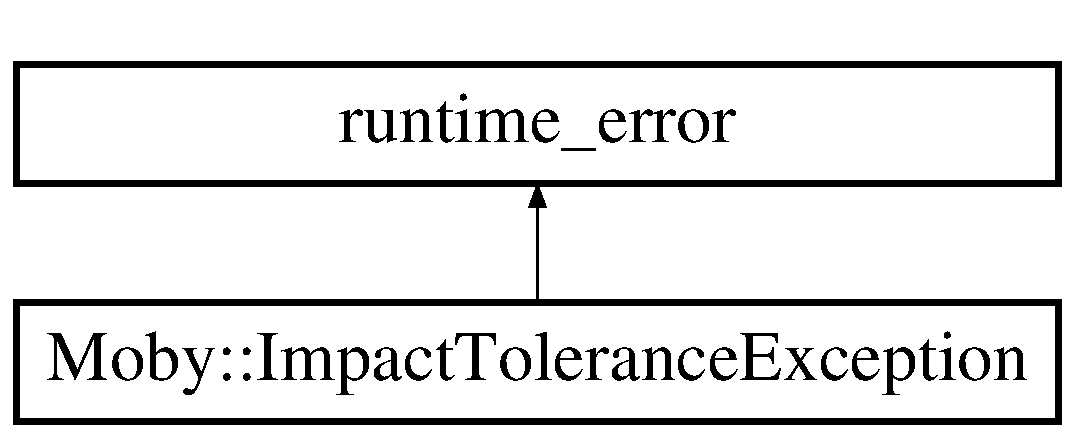
\includegraphics[height=2.000000cm]{classMoby_1_1ImpactToleranceException}
\end{center}
\end{figure}
\subsection*{Public Member Functions}
\begin{DoxyCompactItemize}
\item 
{\bfseries Impact\-Tolerance\-Exception} (const std\-::list$<$ {\bf Unilateral\-Constraint} $\ast$ $>$ \&impacting\-\_\-constraints, double max\-\_\-vio)\label{classMoby_1_1ImpactToleranceException_a2ee5b0db75e99e7c98a6c108df8df469}

\end{DoxyCompactItemize}
\subsection*{Public Attributes}
\begin{DoxyCompactItemize}
\item 
std\-::list$<$ {\bf Unilateral\-Constraint} $\ast$ $>$ {\bfseries constraints}\label{classMoby_1_1ImpactToleranceException_afa84ee489c09193673a1c1dabefe529e}

\item 
double {\bfseries violation}\label{classMoby_1_1ImpactToleranceException_a0364fea9c586d2feddbdbc06c08ddf70}

\end{DoxyCompactItemize}


\subsection{Detailed Description}
Exception thrown when constraint violation is greater than a desired tolerance. 

The documentation for this class was generated from the following file\-:\begin{DoxyCompactItemize}
\item 
/home/drum/\-Moby/include/\-Moby/Impact\-Tolerance\-Exception.\-h\end{DoxyCompactItemize}

\section{Moby\-:\-:Indexed\-Tri Struct Reference}
\label{structMoby_1_1IndexedTri}\index{Moby\-::\-Indexed\-Tri@{Moby\-::\-Indexed\-Tri}}


An indexed triangle.  




{\ttfamily \#include $<$Indexed\-Tri.\-h$>$}

\subsection*{Public Member Functions}
\begin{DoxyCompactItemize}
\item 
{\bfseries Indexed\-Tri} (unsigned v1, unsigned v2, unsigned v3)\label{structMoby_1_1IndexedTri_ac3728317292fe2f795832f2f8a79bfe5}

\item 
{\bf Indexed\-Tri} \& {\bf reverse} ()\label{structMoby_1_1IndexedTri_a3074586a266fdfd428905eec08599c9c}

\begin{DoxyCompactList}\small\item\em Reverses the orientation of the triangle. \end{DoxyCompactList}\item 
bool {\bfseries operator$<$} (const {\bf Indexed\-Tri} \&t) const \label{structMoby_1_1IndexedTri_a9a408cc6d9b7a939845c18edf06becb6}

\end{DoxyCompactItemize}
\subsection*{Public Attributes}
\begin{DoxyCompactItemize}
\item 
unsigned {\bf a}\label{structMoby_1_1IndexedTri_a7193bb478121ac18c21914de18a1f98e}

\begin{DoxyCompactList}\small\item\em Index of the first vertex of the triangle. \end{DoxyCompactList}\item 
unsigned {\bf b}\label{structMoby_1_1IndexedTri_aa00df5b74277e5cf2eec276dbbd15809}

\begin{DoxyCompactList}\small\item\em Index of the second vertex of the triangle. \end{DoxyCompactList}\item 
unsigned {\bf c}\label{structMoby_1_1IndexedTri_a60744804b3de6111e0c7705999a9e3a4}

\begin{DoxyCompactList}\small\item\em Index of the third vertex of the triangle. \end{DoxyCompactList}\end{DoxyCompactItemize}


\subsection{Detailed Description}
An indexed triangle. 

The documentation for this struct was generated from the following file\-:\begin{DoxyCompactItemize}
\item 
/home/drum/\-Moby/include/\-Moby/Indexed\-Tri.\-h\end{DoxyCompactItemize}

\section{Moby\-:\-:Indexed\-Tri\-Array Class Reference}
\label{classMoby_1_1IndexedTriArray}\index{Moby\-::\-Indexed\-Tri\-Array@{Moby\-::\-Indexed\-Tri\-Array}}


An array of triangles indexed into shared vertices.  




{\ttfamily \#include $<$Indexed\-Tri\-Array.\-h$>$}

\subsection*{Public Member Functions}
\begin{DoxyCompactItemize}
\item 
{\bfseries Indexed\-Tri\-Array} (boost\-::shared\-\_\-ptr$<$ const std\-::vector$<$ Ravelin\-::\-Origin3d $>$ $>$ vertices, const std\-::vector$<$ {\bf Indexed\-Tri} $>$ \&facets)\label{classMoby_1_1IndexedTriArray_a22bc8543dd13db0238cb80b08fff0484}

\item 
{\bfseries Indexed\-Tri\-Array} (boost\-::shared\-\_\-ptr$<$ const std\-::vector$<$ Ravelin\-::\-Origin3d $>$ $>$ vertices, boost\-::shared\-\_\-ptr$<$ const std\-::vector$<$ {\bf Indexed\-Tri} $>$ $>$ facets)\label{classMoby_1_1IndexedTriArray_aa886b9d42b2e5d3b610f4ee649fd77b8}

\item 
{\footnotesize template$<$class Forward\-Iterator1 , class Forward\-Iterator2 $>$ }\\{\bf Indexed\-Tri\-Array} (Forward\-Iterator1 vertices, Forward\-Iterator1 verts\-\_\-end, Forward\-Iterator2 facets\-\_\-begin, Forward\-Iterator2 facets\-\_\-end)
\begin{DoxyCompactList}\small\item\em Creates an indexed triangle mesh from containers of vertices and facets. \end{DoxyCompactList}\item 
{\footnotesize template$<$class Output\-Iterator $>$ }\\Output\-Iterator {\bf get\-\_\-tris} (Output\-Iterator output\-\_\-begin, boost\-::shared\-\_\-ptr$<$ const Ravelin\-::\-Pose3d $>$ P) const \label{classMoby_1_1IndexedTriArray_a6cc28fe1ba69b1890ce7d282748d510c}

\begin{DoxyCompactList}\small\item\em Converts an indexed triangle mesh to a container of triangles. \end{DoxyCompactList}\item 
unsigned {\bfseries num\-\_\-tris} () const \label{classMoby_1_1IndexedTriArray_af5b749ac6544676b390da254bce6a031}

\item 
Triangle {\bf get\-\_\-triangle} (unsigned i, boost\-::shared\-\_\-ptr$<$ const Ravelin\-::\-Pose3d $>$ P) const \label{classMoby_1_1IndexedTriArray_a16489b4bc4467ca28b0e633d16f0c56b}

\begin{DoxyCompactList}\small\item\em Gets the i'th triangle from this mesh. \end{DoxyCompactList}\item 
{\bf Indexed\-Tri\-Array} {\bf transform} (const Ravelin\-::\-Transform3d \&T) const \label{classMoby_1_1IndexedTriArray_ae4fc00db00077b5d4d33c92831f21ad3}

\begin{DoxyCompactList}\small\item\em Transforms this mesh to a new mesh. \end{DoxyCompactList}\item 
{\bf Indexed\-Tri\-Array} {\bf compress\-\_\-vertices} () const \label{classMoby_1_1IndexedTriArray_a37fec43458e96f2e785b3a35fc0f1def}

\begin{DoxyCompactList}\small\item\em Compresses the vertices used in an \doxyref{Indexed\-Tri\-Array}{p.}{classMoby_1_1IndexedTriArray} to create a new mesh. \end{DoxyCompactList}\item 
void {\bfseries write\-\_\-to\-\_\-obj} (const std\-::string \&filename) const \label{classMoby_1_1IndexedTriArray_a0227a7d0f0e7c28f72bf9e7c38636b83}

\item 
{\bf Indexed\-Tri\-Array} \& {\bf operator=} (const {\bf Indexed\-Tri\-Array} \&mesh)\label{classMoby_1_1IndexedTriArray_a9f6554fc8f73927a85265a7d30574850}

\begin{DoxyCompactList}\small\item\em Copies one mesh to another. \end{DoxyCompactList}\item 
std\-::vector$<$ std\-::list\\*
$<$ unsigned $>$ $>$ {\bf determine\-\_\-vertex\-\_\-edge\-\_\-map} () const 
\begin{DoxyCompactList}\small\item\em Determines a map from vertices to edges. \end{DoxyCompactList}\item 
std\-::vector$<$ std\-::list\\*
$<$ unsigned $>$ $>$ {\bf determine\-\_\-vertex\-\_\-facet\-\_\-map} () const \label{classMoby_1_1IndexedTriArray_abe943acd02d88d27eef8affa9947ba4a}

\begin{DoxyCompactList}\small\item\em Determines a map from vertices to facet indices. \end{DoxyCompactList}\item 
std\-::map$<$ Ravelin\-::sorted\-\_\-pair\\*
$<$ unsigned $>$, std\-::list\\*
$<$ unsigned $>$ $>$ {\bf determine\-\_\-edge\-\_\-facet\-\_\-map} () const \label{classMoby_1_1IndexedTriArray_a7ec78943c2c285fff89acac35f929ca5}

\begin{DoxyCompactList}\small\item\em Determines a map from edges to facet indices. \end{DoxyCompactList}\item 
void {\bf calc\-\_\-volume\-\_\-ints} (double volume\-\_\-ints[10]) const \label{classMoby_1_1IndexedTriArray_a2548fec85bdafe3bf0bd0efd216c6c25}

\begin{DoxyCompactList}\small\item\em Calculates the volume integrals of this primitive as a triangle mesh. \end{DoxyCompactList}\item 
const std\-::list$<$ unsigned $>$ \& {\bf get\-\_\-incident\-\_\-facets} (unsigned i) const \label{classMoby_1_1IndexedTriArray_aa4e59c05403b17345c3e64d0f1f76663}

\begin{DoxyCompactList}\small\item\em Gets the indices of facets incident to a vertex. \end{DoxyCompactList}\item 
boost\-::shared\-\_\-ptr$<$ const \\*
std\-::vector$<$ {\bf Indexed\-Tri} $>$ $>$ {\bf get\-\_\-facets\-\_\-pointer} () const \label{classMoby_1_1IndexedTriArray_a28944f0e2e4608939ad0b0f539f57123}

\begin{DoxyCompactList}\small\item\em Gets the pointer to the vector of facets. \end{DoxyCompactList}\item 
boost\-::shared\-\_\-ptr$<$ const \\*
std\-::vector$<$ Ravelin\-::\-Origin3d $>$ $>$ {\bf get\-\_\-vertices\-\_\-pointer} () const \label{classMoby_1_1IndexedTriArray_abfeae4937eafc2411d2b904751a1941b}

\begin{DoxyCompactList}\small\item\em Gets the pointer to the vector of vertices. \end{DoxyCompactList}\item 
const std\-::vector$<$ {\bf Indexed\-Tri} $>$ \& {\bf get\-\_\-facets} () const \label{classMoby_1_1IndexedTriArray_a649f40490ab06039203a73d7777bfe9f}

\begin{DoxyCompactList}\small\item\em Gets the vector of facets. \end{DoxyCompactList}\item 
const std\-::vector\\*
$<$ Ravelin\-::\-Origin3d $>$ \& {\bf get\-\_\-vertices} () const \label{classMoby_1_1IndexedTriArray_ad4ab695884f00df367e8e8f9fd17f9e2}

\begin{DoxyCompactList}\small\item\em Gets the vector of verties. \end{DoxyCompactList}\item 
bool {\bf is\-\_\-coplanar} (unsigned vidx) const \label{classMoby_1_1IndexedTriArray_a4471d53875e96208021b0a194d492ca2}

\begin{DoxyCompactList}\small\item\em Determines whether a vertex is coplanar (all faces touching the vertex are coplanar) \end{DoxyCompactList}\item 
bool {\bf is\-\_\-coplanar} (unsigned v1, unsigned v2) const \label{classMoby_1_1IndexedTriArray_a59b5cfa70967fb368d56ea24fa4a96b2}

\begin{DoxyCompactList}\small\item\em Determines whether an edge (v1,v2) is coplanar (all faces touching the edge are coplanar) \end{DoxyCompactList}\item 
{\footnotesize template$<$class Forward\-Iterator1 , class Forward\-Iterator2 $>$ }\\{\bf Indexed\-Tri\-Array} (Forward\-Iterator1 verts\-\_\-begin, Forward\-Iterator1 verts\-\_\-end, Forward\-Iterator2 facets\-\_\-begin, Forward\-Iterator2 facets\-\_\-end)
\begin{DoxyCompactList}\small\item\em Creates an indexed triangle mesh from containers of vertices and facets. \end{DoxyCompactList}\item 
{\footnotesize template$<$class Output\-Iterator $>$ }\\Output\-Iterator {\bf get\-\_\-tris} (Output\-Iterator output\-\_\-begin, boost\-::shared\-\_\-ptr$<$ const Ravelin\-::\-Pose3d $>$ P) const \label{classMoby_1_1IndexedTriArray_a6cc28fe1ba69b1890ce7d282748d510c}

\begin{DoxyCompactList}\small\item\em Converts an indexed triangle mesh to a container of triangles. \end{DoxyCompactList}\item 
{\footnotesize template$<$class Output\-Iterator $>$ }\\Output\-Iterator {\bf intersect} (const {\bf Indexed\-Tri\-Array} \&mesh\-\_\-a, const {\bf Indexed\-Tri\-Array} \&mesh\-\_\-b, Output\-Iterator output\-\_\-begin, boost\-::shared\-\_\-ptr$<$ const Ravelin\-::\-Pose3d $>$ Pa, boost\-::shared\-\_\-ptr$<$ const Ravelin\-::\-Pose3d $>$ Pb, bool exit\-\_\-early)
\begin{DoxyCompactList}\small\item\em Intersects two meshes together and returns indices of intersecting triangles. \end{DoxyCompactList}\end{DoxyCompactItemize}
\subsection*{Static Public Member Functions}
\begin{DoxyCompactItemize}
\item 
{\footnotesize template$<$class Output\-Iterator $>$ }\\static Output\-Iterator {\bf intersect} (const {\bf Indexed\-Tri\-Array} \&mesh\-\_\-a, const {\bf Indexed\-Tri\-Array} \&mesh\-\_\-b, Output\-Iterator output\-\_\-begin, boost\-::shared\-\_\-ptr$<$ const Ravelin\-::\-Pose3d $>$ Pa, boost\-::shared\-\_\-ptr$<$ const Ravelin\-::\-Pose3d $>$ Pb, bool exit\-\_\-early)
\begin{DoxyCompactList}\small\item\em Intersects two meshes together and returns indices of intersecting triangles. \end{DoxyCompactList}\item 
static {\bf Indexed\-Tri\-Array} {\bf read\-\_\-from\-\_\-obj} (const std\-::string \&filename)\label{classMoby_1_1IndexedTriArray_a0c0d473f0a2f0fc7f96088adcf2f6f68}

\begin{DoxyCompactList}\small\item\em Reads triangle mesh from a Wavefront O\-B\-J file. \end{DoxyCompactList}\item 
static void {\bfseries write\-\_\-to\-\_\-obj} (const {\bf Indexed\-Tri\-Array} \&mesh, const std\-::string \&filename)\label{classMoby_1_1IndexedTriArray_a152732a80d0847cbacd681a0bec263c2}

\item 
static {\bf Indexed\-Tri\-Array} {\bf merge} (const {\bf Indexed\-Tri\-Array} \&mesh1, const {\bf Indexed\-Tri\-Array} \&mesh2, double equal\-\_\-tol=0.\-0)
\begin{DoxyCompactList}\small\item\em Merges two meshes together to create a new mesh. \end{DoxyCompactList}\end{DoxyCompactItemize}


\subsection{Detailed Description}
An array of triangles indexed into shared vertices. 

\subsection{Constructor \& Destructor Documentation}
\index{Moby\-::\-Indexed\-Tri\-Array@{Moby\-::\-Indexed\-Tri\-Array}!Indexed\-Tri\-Array@{Indexed\-Tri\-Array}}
\index{Indexed\-Tri\-Array@{Indexed\-Tri\-Array}!Moby::IndexedTriArray@{Moby\-::\-Indexed\-Tri\-Array}}
\subsubsection[{Indexed\-Tri\-Array}]{\setlength{\rightskip}{0pt plus 5cm}template$<$class Forward\-Iterator1 , class Forward\-Iterator2 $>$ Moby\-::\-Indexed\-Tri\-Array\-::\-Indexed\-Tri\-Array (
\begin{DoxyParamCaption}
\item[{Forward\-Iterator1}]{verts\-\_\-begin, }
\item[{Forward\-Iterator1}]{verts\-\_\-end, }
\item[{Forward\-Iterator2}]{facets\-\_\-begin, }
\item[{Forward\-Iterator2}]{facets\-\_\-end}
\end{DoxyParamCaption}
)}\label{classMoby_1_1IndexedTriArray_a3945b2075099e0b41cdcaec73deaf98f}


Creates an indexed triangle mesh from containers of vertices and facets. 


\begin{DoxyParams}{Parameters}
{\em vertices} & an iterator to the beginning of a container of Point3d objects \\
\hline
{\em verts\-\_\-end} & an iterator to the end of a container of Point3d objects \\
\hline
{\em facets\-\_\-begin} & an iterator to the beginning of a container of \doxyref{Indexed\-Tri}{p.}{structMoby_1_1IndexedTri} objects \\
\hline
{\em facets\-\_\-end} & an iterator to the end of a container of \doxyref{Indexed\-Tri}{p.}{structMoby_1_1IndexedTri} objects \\
\hline
\end{DoxyParams}
\index{Moby\-::\-Indexed\-Tri\-Array@{Moby\-::\-Indexed\-Tri\-Array}!Indexed\-Tri\-Array@{Indexed\-Tri\-Array}}
\index{Indexed\-Tri\-Array@{Indexed\-Tri\-Array}!Moby::IndexedTriArray@{Moby\-::\-Indexed\-Tri\-Array}}
\subsubsection[{Indexed\-Tri\-Array}]{\setlength{\rightskip}{0pt plus 5cm}template$<$class Forward\-Iterator1 , class Forward\-Iterator2 $>$ Moby\-::\-Indexed\-Tri\-Array\-::\-Indexed\-Tri\-Array (
\begin{DoxyParamCaption}
\item[{Forward\-Iterator1}]{verts\-\_\-begin, }
\item[{Forward\-Iterator1}]{verts\-\_\-end, }
\item[{Forward\-Iterator2}]{facets\-\_\-begin, }
\item[{Forward\-Iterator2}]{facets\-\_\-end}
\end{DoxyParamCaption}
)}\label{classMoby_1_1IndexedTriArray_a8c9bb0ca489c52ef328939dc4b9f8bb5}


Creates an indexed triangle mesh from containers of vertices and facets. 


\begin{DoxyParams}{Parameters}
{\em vertices} & an iterator to the beginning of a container of Point3d objects \\
\hline
{\em verts\-\_\-end} & an iterator to the end of a container of Point3d objects \\
\hline
{\em facets\-\_\-begin} & an iterator to the beginning of a container of \doxyref{Indexed\-Tri}{p.}{structMoby_1_1IndexedTri} objects \\
\hline
{\em facets\-\_\-end} & an iterator to the end of a container of \doxyref{Indexed\-Tri}{p.}{structMoby_1_1IndexedTri} objects \\
\hline
\end{DoxyParams}


\subsection{Member Function Documentation}
\index{Moby\-::\-Indexed\-Tri\-Array@{Moby\-::\-Indexed\-Tri\-Array}!determine\-\_\-vertex\-\_\-edge\-\_\-map@{determine\-\_\-vertex\-\_\-edge\-\_\-map}}
\index{determine\-\_\-vertex\-\_\-edge\-\_\-map@{determine\-\_\-vertex\-\_\-edge\-\_\-map}!Moby::IndexedTriArray@{Moby\-::\-Indexed\-Tri\-Array}}
\subsubsection[{determine\-\_\-vertex\-\_\-edge\-\_\-map}]{\setlength{\rightskip}{0pt plus 5cm}vector$<$ list$<$ unsigned $>$ $>$ Indexed\-Tri\-Array\-::determine\-\_\-vertex\-\_\-edge\-\_\-map (
\begin{DoxyParamCaption}
{}
\end{DoxyParamCaption}
) const}\label{classMoby_1_1IndexedTriArray_a1a57addac80e6a8d74ddc81caff82e1a}


Determines a map from vertices to edges. 

\begin{DoxyReturn}{Returns}
a map from vertices to edges; each element in the map repesents the second vertex of the edge (the key is the first) 
\end{DoxyReturn}


Referenced by Moby\-::\-O\-B\-B\-::calc\-\_\-min\-\_\-volume\-\_\-\-O\-B\-B().

\index{Moby\-::\-Indexed\-Tri\-Array@{Moby\-::\-Indexed\-Tri\-Array}!intersect@{intersect}}
\index{intersect@{intersect}!Moby::IndexedTriArray@{Moby\-::\-Indexed\-Tri\-Array}}
\subsubsection[{intersect}]{\setlength{\rightskip}{0pt plus 5cm}template$<$class Output\-Iterator $>$ Output\-Iterator Moby\-::\-Indexed\-Tri\-Array\-::intersect (
\begin{DoxyParamCaption}
\item[{const {\bf Indexed\-Tri\-Array} \&}]{mesh\-\_\-a, }
\item[{const {\bf Indexed\-Tri\-Array} \&}]{mesh\-\_\-b, }
\item[{Output\-Iterator}]{output\-\_\-begin, }
\item[{boost\-::shared\-\_\-ptr$<$ const Ravelin\-::\-Pose3d $>$}]{Pa, }
\item[{boost\-::shared\-\_\-ptr$<$ const Ravelin\-::\-Pose3d $>$}]{Pb, }
\item[{bool}]{exit\-\_\-early}
\end{DoxyParamCaption}
)\hspace{0.3cm}{\ttfamily [static]}}\label{classMoby_1_1IndexedTriArray_a1ea78f2d40caf44c843dc67ecd7472b5}


Intersects two meshes together and returns indices of intersecting triangles. 


\begin{DoxyParams}{Parameters}
{\em mesh\-\_\-a} & the first mesh \\
\hline
{\em mesh\-\_\-b} & the second mesh \\
\hline
{\em output\-\_\-begin} & an iterator pointing to the beginning of a container of std\-::pair$<$unsigned, unsigned$>$ objects (on return, container will hold indices of intersecting triangles of mesh\-\_\-a and mesh\-\_\-b) \\
\hline
{\em exit\-\_\-early} & if {\bfseries true}, exits after first intersection detected \\
\hline
\end{DoxyParams}
\begin{DoxyReturn}{Returns}
an iterator pointing to the end of a container of std\-::pair$<$unsigned, unsigned$>$ objects (on return, container will hold indices of intersecting triangles of mesh\-\_\-a and mesh\-\_\-b) 
\end{DoxyReturn}
\index{Moby\-::\-Indexed\-Tri\-Array@{Moby\-::\-Indexed\-Tri\-Array}!intersect@{intersect}}
\index{intersect@{intersect}!Moby::IndexedTriArray@{Moby\-::\-Indexed\-Tri\-Array}}
\subsubsection[{intersect}]{\setlength{\rightskip}{0pt plus 5cm}template$<$class Output\-Iterator $>$ Output\-Iterator Moby\-::\-Indexed\-Tri\-Array\-::intersect (
\begin{DoxyParamCaption}
\item[{const {\bf Indexed\-Tri\-Array} \&}]{mesh\-\_\-a, }
\item[{const {\bf Indexed\-Tri\-Array} \&}]{mesh\-\_\-b, }
\item[{Output\-Iterator}]{output\-\_\-begin, }
\item[{boost\-::shared\-\_\-ptr$<$ const Ravelin\-::\-Pose3d $>$}]{Pa, }
\item[{boost\-::shared\-\_\-ptr$<$ const Ravelin\-::\-Pose3d $>$}]{Pb, }
\item[{bool}]{exit\-\_\-early}
\end{DoxyParamCaption}
)}\label{classMoby_1_1IndexedTriArray_a1ea78f2d40caf44c843dc67ecd7472b5}


Intersects two meshes together and returns indices of intersecting triangles. 


\begin{DoxyParams}{Parameters}
{\em mesh\-\_\-a} & the first mesh \\
\hline
{\em mesh\-\_\-b} & the second mesh \\
\hline
{\em output\-\_\-begin} & an iterator pointing to the beginning of a container of std\-::pair$<$unsigned, unsigned$>$ objects (on return, container will hold indices of intersecting triangles of mesh\-\_\-a and mesh\-\_\-b) \\
\hline
{\em exit\-\_\-early} & if {\bfseries true}, exits after first intersection detected \\
\hline
\end{DoxyParams}
\begin{DoxyReturn}{Returns}
an iterator pointing to the end of a container of std\-::pair$<$unsigned, unsigned$>$ objects (on return, container will hold indices of intersecting triangles of mesh\-\_\-a and mesh\-\_\-b) 
\end{DoxyReturn}


References get\-\_\-tris().

\index{Moby\-::\-Indexed\-Tri\-Array@{Moby\-::\-Indexed\-Tri\-Array}!merge@{merge}}
\index{merge@{merge}!Moby::IndexedTriArray@{Moby\-::\-Indexed\-Tri\-Array}}
\subsubsection[{merge}]{\setlength{\rightskip}{0pt plus 5cm}{\bf Indexed\-Tri\-Array} Indexed\-Tri\-Array\-::merge (
\begin{DoxyParamCaption}
\item[{const {\bf Indexed\-Tri\-Array} \&}]{mesh1, }
\item[{const {\bf Indexed\-Tri\-Array} \&}]{mesh2, }
\item[{double}]{equal\-\_\-tol = {\ttfamily 0.0}}
\end{DoxyParamCaption}
)\hspace{0.3cm}{\ttfamily [static]}}\label{classMoby_1_1IndexedTriArray_a3a9a4d32a18987a780a8494ff9af5fe0}


Merges two meshes together to create a new mesh. 

\begin{DoxyNote}{Note}
this method runs in time O(nm) 
\end{DoxyNote}


References get\-\_\-facets(), and get\-\_\-vertices().



The documentation for this class was generated from the following files\-:\begin{DoxyCompactItemize}
\item 
/home/drum/\-Moby/include/\-Moby/Indexed\-Tri\-Array.\-h\item 
/home/drum/\-Moby/include/\-Moby/Indexed\-Tri\-Array.\-inl\item 
/home/drum/\-Moby/src/Indexed\-Tri\-Array.\-cpp\end{DoxyCompactItemize}

\section{Moby\-:\-:Invalid\-Index\-Exception Class Reference}
\label{classMoby_1_1InvalidIndexException}\index{Moby\-::\-Invalid\-Index\-Exception@{Moby\-::\-Invalid\-Index\-Exception}}


Exception thrown when trying to access the index beyond the range of the data.  




{\ttfamily \#include $<$Invalid\-Index\-Exception.\-h$>$}

Inheritance diagram for Moby\-:\-:Invalid\-Index\-Exception\-:\begin{figure}[H]
\begin{center}
\leavevmode
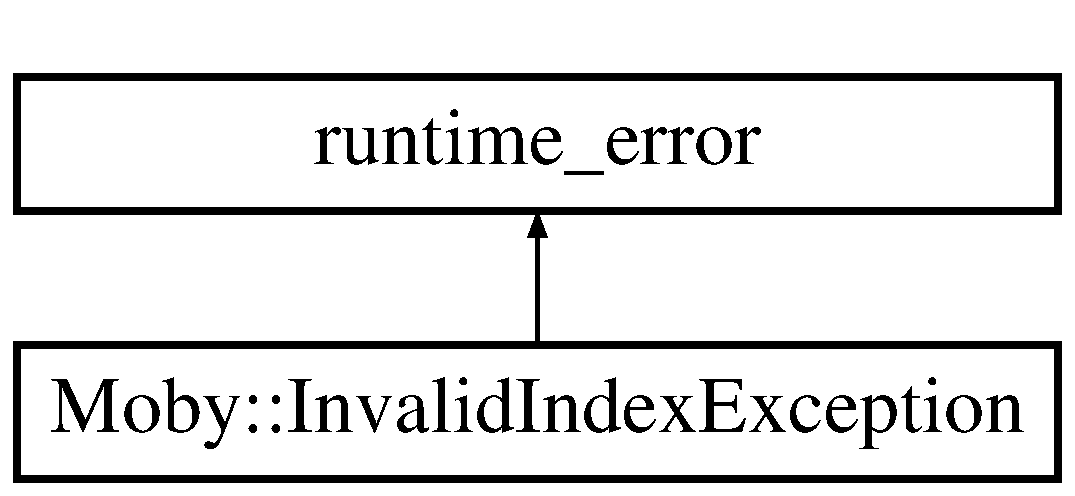
\includegraphics[height=2.000000cm]{classMoby_1_1InvalidIndexException}
\end{center}
\end{figure}


\subsection{Detailed Description}
Exception thrown when trying to access the index beyond the range of the data. 

The documentation for this class was generated from the following file\-:\begin{DoxyCompactItemize}
\item 
/home/drum/\-Moby/include/\-Moby/Invalid\-Index\-Exception.\-h\end{DoxyCompactItemize}

\section{Moby\-:\-:Invalid\-State\-Exception Class Reference}
\label{classMoby_1_1InvalidStateException}\index{Moby\-::\-Invalid\-State\-Exception@{Moby\-::\-Invalid\-State\-Exception}}


Exception thrown when an integrator tries to evaluate a derivative at an invalid state.  




{\ttfamily \#include $<$Invalid\-State\-Exception.\-h$>$}

Inheritance diagram for Moby\-:\-:Invalid\-State\-Exception\-:\begin{figure}[H]
\begin{center}
\leavevmode
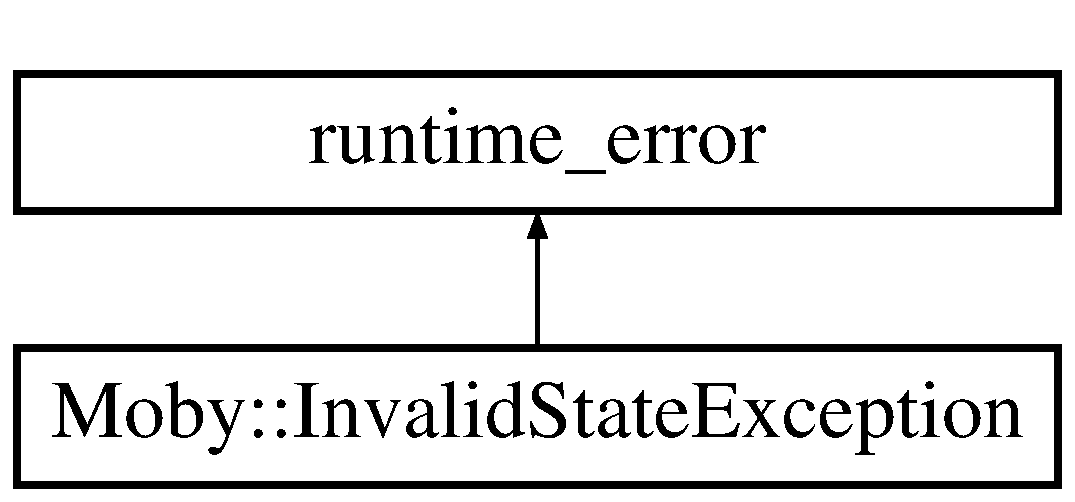
\includegraphics[height=2.000000cm]{classMoby_1_1InvalidStateException}
\end{center}
\end{figure}
\subsection*{Public Member Functions}
\begin{DoxyCompactItemize}
\item 
{\bfseries Invalid\-State\-Exception} (const char $\ast$error)\label{classMoby_1_1InvalidStateException_ac486490708afd97dd3babf746cdefcf8}

\end{DoxyCompactItemize}


\subsection{Detailed Description}
Exception thrown when an integrator tries to evaluate a derivative at an invalid state. 

The documentation for this class was generated from the following file\-:\begin{DoxyCompactItemize}
\item 
/home/drum/\-Moby/include/\-Moby/Invalid\-State\-Exception.\-h\end{DoxyCompactItemize}

\section{Moby\-:\-:Invalid\-Velocity\-Exception Class Reference}
\label{classMoby_1_1InvalidVelocityException}\index{Moby\-::\-Invalid\-Velocity\-Exception@{Moby\-::\-Invalid\-Velocity\-Exception}}


Exception thrown when an integrator tries to evaluate a derivative at an invalid velocity.  




{\ttfamily \#include $<$Invalid\-Velocity\-Exception.\-h$>$}

Inheritance diagram for Moby\-:\-:Invalid\-Velocity\-Exception\-:\begin{figure}[H]
\begin{center}
\leavevmode
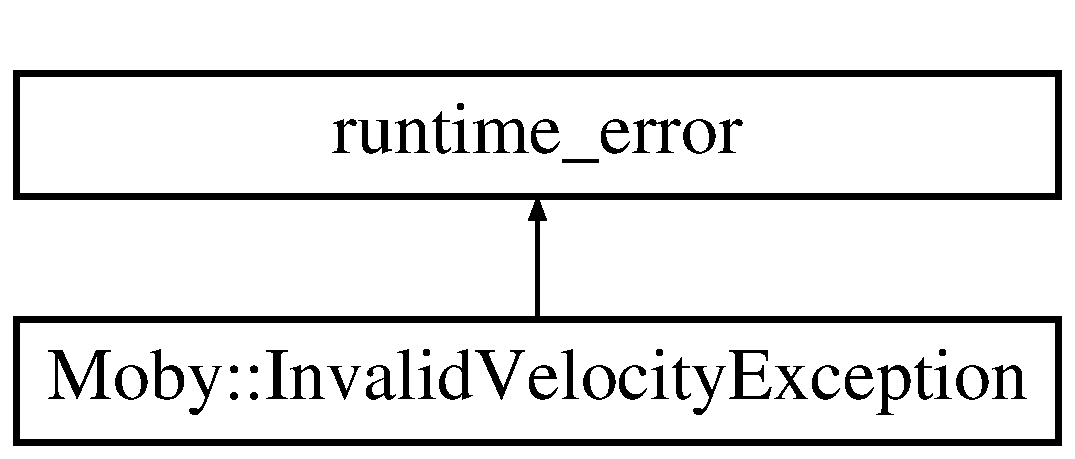
\includegraphics[height=2.000000cm]{classMoby_1_1InvalidVelocityException}
\end{center}
\end{figure}
\subsection*{Public Member Functions}
\begin{DoxyCompactItemize}
\item 
{\bfseries Invalid\-Velocity\-Exception} (double t)\label{classMoby_1_1InvalidVelocityException_ac1fd7df3c0891e04b2292ee51c119163}

\end{DoxyCompactItemize}
\subsection*{Public Attributes}
\begin{DoxyCompactItemize}
\item 
double {\bfseries evaluation\-\_\-time}\label{classMoby_1_1InvalidVelocityException_a414ec52bc7893290faa3595d1c9a7518}

\end{DoxyCompactItemize}


\subsection{Detailed Description}
Exception thrown when an integrator tries to evaluate a derivative at an invalid velocity. 

The documentation for this class was generated from the following file\-:\begin{DoxyCompactItemize}
\item 
/home/drum/\-Moby/include/\-Moby/Invalid\-Velocity\-Exception.\-h\end{DoxyCompactItemize}

\section{Moby\-:\-:Joint Class Reference}
\label{classMoby_1_1Joint}\index{Moby\-::\-Joint@{Moby\-::\-Joint}}


Defines a joint used in articulated rigid body dynamics simulation.  




{\ttfamily \#include $<$Joint.\-h$>$}

Inheritance diagram for Moby\-:\-:Joint\-:\begin{figure}[H]
\begin{center}
\leavevmode
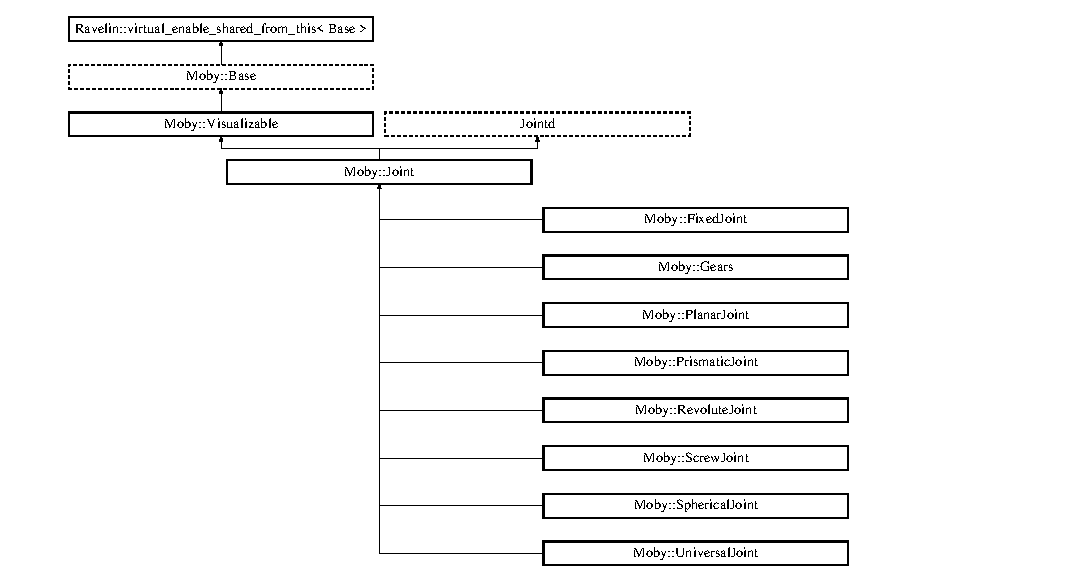
\includegraphics[height=7.368422cm]{classMoby_1_1Joint}
\end{center}
\end{figure}
\subsection*{Public Types}
\begin{DoxyCompactItemize}
\item 
enum {\bf Constraint\-Type} \{ {\bfseries e\-Unknown}, 
{\bfseries e\-Explicit}, 
{\bfseries e\-Implicit}
 \}
\item 
enum {\bfseries D\-O\-Fs} \{ \\*
{\bfseries D\-O\-F\-\_\-1} =0, 
{\bfseries D\-O\-F\-\_\-2} =1, 
{\bfseries D\-O\-F\-\_\-3} =2, 
{\bfseries D\-O\-F\-\_\-4} =3, 
\\*
{\bfseries D\-O\-F\-\_\-5} =4, 
{\bfseries D\-O\-F\-\_\-6} =5
 \}
\end{DoxyCompactItemize}
\subsection*{Public Member Functions}
\begin{DoxyCompactItemize}
\item 
{\bf Joint} ()
\begin{DoxyCompactList}\small\item\em Initializes the joint. \end{DoxyCompactList}\item 
{\bf Joint} (boost\-::weak\-\_\-ptr$<$ {\bf Rigid\-Body} $>$ inboard, boost\-::weak\-\_\-ptr$<$ {\bf Rigid\-Body} $>$ outboard)
\begin{DoxyCompactList}\small\item\em Initializes the joint with the specified inboard and outboard links. \end{DoxyCompactList}\item 
void {\bf set\-\_\-location} (const {\bf Point3d} \&p, {\bf Rigid\-Body\-Ptr} inboard, {\bf Rigid\-Body\-Ptr} outboard)\label{classMoby_1_1Joint_afd574362724420c8efa455fa9b98808a}

\begin{DoxyCompactList}\small\item\em Sets the location of this joint with specified inboard and outboard links. \end{DoxyCompactList}\item 
Ravelin\-::\-Vector\-Nd \& {\bf get\-\_\-scaled\-\_\-force} (Ravelin\-::\-Vector\-Nd \&f)
\begin{DoxyCompactList}\small\item\em Gets the scaled actuator forces. \end{DoxyCompactList}\item 
virtual void {\bf save\-\_\-to\-\_\-xml} ({\bf X\-M\-L\-Tree\-Ptr} node, std\-::list$<$ boost\-::shared\-\_\-ptr$<$ const {\bf Base} $>$ $>$ \&shared\-\_\-objects) const \label{classMoby_1_1Joint_ab5ad56ab0008dfd54a78aa3289854af7}

\begin{DoxyCompactList}\small\item\em Implements \doxyref{Base\-::save\-\_\-to\-\_\-xml()}{p.}{classMoby_1_1Base_aed64905ca39893d02d1e6c3f03f73aa9} \end{DoxyCompactList}\item 
virtual void {\bf load\-\_\-from\-\_\-xml} (boost\-::shared\-\_\-ptr$<$ const {\bf X\-M\-L\-Tree} $>$ node, std\-::map$<$ std\-::string, {\bf Base\-Ptr} $>$ \&id\-\_\-map)\label{classMoby_1_1Joint_a5e0c23575a509a152d212b2b7dc3ffa6}

\begin{DoxyCompactList}\small\item\em Implements \doxyref{Base\-::load\-\_\-from\-\_\-xml()}{p.}{classMoby_1_1Base_a98b861c1d615a748b576aa613f17389f} \end{DoxyCompactList}\item 
virtual void {\bf set\-\_\-inboard\-\_\-link} ({\bf Rigid\-Body\-Ptr} link, bool update\-\_\-pose)\label{classMoby_1_1Joint_a99fa85e0b9d7011b8c68f81b1a6174fd}

\begin{DoxyCompactList}\small\item\em Sets the pointer to the inboard link for this joint (and updates the spatial axes, if the outboard link has been set) \end{DoxyCompactList}\item 
virtual void {\bf set\-\_\-outboard\-\_\-link} ({\bf Rigid\-Body\-Ptr} link, bool update\-\_\-pose)
\begin{DoxyCompactList}\small\item\em Sets the pointer to the outboard link for this joint. \end{DoxyCompactList}\item 
void {\bf set\-\_\-articulated\-\_\-body} ({\bf Articulated\-Body\-Ptr} abody)
\begin{DoxyCompactList}\small\item\em Sets the articulated body corresponding to this body. \end{DoxyCompactList}\item 
{\bf Articulated\-Body\-Ptr} {\bf get\-\_\-articulated\-\_\-body} ()
\begin{DoxyCompactList}\small\item\em Gets the articulated body corresponding to this body. \end{DoxyCompactList}\item 
{\bf Rigid\-Body\-Ptr} {\bf get\-\_\-inboard\-\_\-link} () const \label{classMoby_1_1Joint_ad1568079a879ef854eb3f75eac01a7a4}

\begin{DoxyCompactList}\small\item\em Gets the inboard link for this joint. \end{DoxyCompactList}\item 
{\bf Rigid\-Body\-Ptr} {\bf get\-\_\-outboard\-\_\-link} () const \label{classMoby_1_1Joint_a34ebb19de0943fa0d1b4679fea81ea04}

\begin{DoxyCompactList}\small\item\em Gets the outboard link for this joint. \end{DoxyCompactList}\end{DoxyCompactItemize}
\subsection*{Public Attributes}
\begin{DoxyCompactItemize}
\item 
Ravelin\-::\-Vector\-Nd {\bf lolimit}\label{classMoby_1_1Joint_acabab537c9c909dcbdbce43947880081}

\begin{DoxyCompactList}\small\item\em The lower joint limit. \end{DoxyCompactList}\item 
Ravelin\-::\-Vector\-Nd {\bf hilimit}\label{classMoby_1_1Joint_a19cdc15da08714e00415f5a94fffa50d}

\begin{DoxyCompactList}\small\item\em The upper joint limit. \end{DoxyCompactList}\item 
double {\bf limit\-\_\-restitution}\label{classMoby_1_1Joint_a2eb51b2bd2e2e029794480eb7dfd6e1d}

\begin{DoxyCompactList}\small\item\em The coefficient of restitution applied when this joint reaches a limit. \end{DoxyCompactList}\item 
double {\bf mu\-\_\-fc}\label{classMoby_1_1Joint_a00d23e7dc39568e83c1685a6a244d5ce}

\begin{DoxyCompactList}\small\item\em The coulomb friction coefficient for this joint. \end{DoxyCompactList}\item 
double {\bf mu\-\_\-fv}\label{classMoby_1_1Joint_ad77c028abff83b4e4177f34b2c4fb0c4}

\begin{DoxyCompactList}\small\item\em The viscous friction coefficient for this joint. \end{DoxyCompactList}\item 
double {\bf compliant\-\_\-layer\-\_\-depth}\label{classMoby_1_1Joint_a9989b3b0b92662b7a0d7949334355429}

\begin{DoxyCompactList}\small\item\em The depth of the compliant layer around the joint limit. \end{DoxyCompactList}\end{DoxyCompactItemize}
\subsection*{Protected Member Functions}
\begin{DoxyCompactItemize}
\item 
void {\bf determine\-\_\-q\-\_\-dot} ()\label{classMoby_1_1Joint_abe44fa8bbfec2483a2f73e5729b7e580}

\begin{DoxyCompactList}\small\item\em (Relatively slow) method for determining the joint velocity from current link velocities \end{DoxyCompactList}\item 
virtual void {\bf init\-\_\-data} ()
\begin{DoxyCompactList}\small\item\em Computes the constraint Jacobian for this joint with respect to the given body in Rodrigues parameters. \end{DoxyCompactList}\end{DoxyCompactItemize}
\subsection*{Friends}
\begin{DoxyCompactItemize}
\item 
class {\bfseries Articulated\-Body}\label{classMoby_1_1Joint_a7d29a1ee423a6e8dab5bf1a58b001f17}

\end{DoxyCompactItemize}
\subsection*{Additional Inherited Members}


\subsection{Detailed Description}
Defines a joint used in articulated rigid body dynamics simulation. 

\begin{DoxyRefDesc}{Todo}
\item[{\bf Todo}]implement a rest position for q? \end{DoxyRefDesc}


\subsection{Member Enumeration Documentation}
\index{Moby\-::\-Joint@{Moby\-::\-Joint}!Constraint\-Type@{Constraint\-Type}}
\index{Constraint\-Type@{Constraint\-Type}!Moby::Joint@{Moby\-::\-Joint}}
\subsubsection[{Constraint\-Type}]{\setlength{\rightskip}{0pt plus 5cm}enum {\bf Moby\-::\-Joint\-::\-Constraint\-Type}}\label{classMoby_1_1Joint_aea02c1460a96e29fdc5fa9bc82c77d1d}
The constraint type is implicit if constraint forces must be determined to hold the inner and outer links together and explicit otherwise. 

\subsection{Constructor \& Destructor Documentation}
\index{Moby\-::\-Joint@{Moby\-::\-Joint}!Joint@{Joint}}
\index{Joint@{Joint}!Moby::Joint@{Moby\-::\-Joint}}
\subsubsection[{Joint}]{\setlength{\rightskip}{0pt plus 5cm}Joint\-::\-Joint (
\begin{DoxyParamCaption}
{}
\end{DoxyParamCaption}
)}\label{classMoby_1_1Joint_a79a7a4715b2166714e039d7c7c5ea3b4}


Initializes the joint. 

The inboard and outboard links are set to N\-U\-L\-L. 

References Moby\-::\-Visualizable\-::\-\_\-v\-F, compliant\-\_\-layer\-\_\-depth, limit\-\_\-restitution, mu\-\_\-fc, and mu\-\_\-fv.

\index{Moby\-::\-Joint@{Moby\-::\-Joint}!Joint@{Joint}}
\index{Joint@{Joint}!Moby::Joint@{Moby\-::\-Joint}}
\subsubsection[{Joint}]{\setlength{\rightskip}{0pt plus 5cm}Joint\-::\-Joint (
\begin{DoxyParamCaption}
\item[{boost\-::weak\-\_\-ptr$<$ {\bf Rigid\-Body} $>$}]{inboard, }
\item[{boost\-::weak\-\_\-ptr$<$ {\bf Rigid\-Body} $>$}]{outboard}
\end{DoxyParamCaption}
)}\label{classMoby_1_1Joint_ae1909595061a35c097bd3f5f4532ddee}


Initializes the joint with the specified inboard and outboard links. 

\begin{DoxyNote}{Note}
does not set the inner joint for the outboard link or add the outboard as a child of the inboard link 
\end{DoxyNote}


References Moby\-::\-Visualizable\-::\-\_\-v\-F, compliant\-\_\-layer\-\_\-depth, limit\-\_\-restitution, mu\-\_\-fc, and mu\-\_\-fv.



\subsection{Member Function Documentation}
\index{Moby\-::\-Joint@{Moby\-::\-Joint}!get\-\_\-articulated\-\_\-body@{get\-\_\-articulated\-\_\-body}}
\index{get\-\_\-articulated\-\_\-body@{get\-\_\-articulated\-\_\-body}!Moby::Joint@{Moby\-::\-Joint}}
\subsubsection[{get\-\_\-articulated\-\_\-body}]{\setlength{\rightskip}{0pt plus 5cm}{\bf Articulated\-Body\-Ptr} Joint\-::get\-\_\-articulated\-\_\-body (
\begin{DoxyParamCaption}
{}
\end{DoxyParamCaption}
)}\label{classMoby_1_1Joint_abb7699b566e8670182a27cec6647804a}


Gets the articulated body corresponding to this body. 

\begin{DoxyReturn}{Returns}
a pointer to the articulated body, or N\-U\-L\-L if this body is not a link an articulated body 
\end{DoxyReturn}
\index{Moby\-::\-Joint@{Moby\-::\-Joint}!get\-\_\-scaled\-\_\-force@{get\-\_\-scaled\-\_\-force}}
\index{get\-\_\-scaled\-\_\-force@{get\-\_\-scaled\-\_\-force}!Moby::Joint@{Moby\-::\-Joint}}
\subsubsection[{get\-\_\-scaled\-\_\-force}]{\setlength{\rightskip}{0pt plus 5cm}Vector\-Nd \& Joint\-::get\-\_\-scaled\-\_\-force (
\begin{DoxyParamCaption}
\item[{Ravelin\-::\-Vector\-Nd \&}]{f}
\end{DoxyParamCaption}
)}\label{classMoby_1_1Joint_a07406fd8c0e415fbfbee5f090a872912}


Gets the scaled actuator forces. 

\begin{DoxyNote}{Note}
relevant only to reduced-\/coordinate articulated bodies 
\end{DoxyNote}
\index{Moby\-::\-Joint@{Moby\-::\-Joint}!init\-\_\-data@{init\-\_\-data}}
\index{init\-\_\-data@{init\-\_\-data}!Moby::Joint@{Moby\-::\-Joint}}
\subsubsection[{init\-\_\-data}]{\setlength{\rightskip}{0pt plus 5cm}void Joint\-::init\-\_\-data (
\begin{DoxyParamCaption}
{}
\end{DoxyParamCaption}
)\hspace{0.3cm}{\ttfamily [protected]}, {\ttfamily [virtual]}}\label{classMoby_1_1Joint_ae884303111aa3dc7700bda55d70b38eb}


Computes the constraint Jacobian for this joint with respect to the given body in Rodrigues parameters. 

Sets the number of degrees-\/of-\/freedom for this joint.


\begin{DoxyParams}{Parameters}
{\em body} & the body with which the constraint Jacobian will be calculated; if the body is not either the inner or outer link, the constraint Jacobian will be a zero matrix \\
\hline
{\em index} & the index of the constraint equation for which to calculate \\
\hline
{\em Cq} & a vector that contains the corresponding column of the constraint Jacobian on return\-Computes the time derivative of the constraint Jacobian for this joint with respect to the given body in Rodrigues parameters \\
\hline
{\em body} & the body with which the constraint Jacobian will be calculated; if the body is not either the inner or outer link, the constraint Jacobian will be a zero matrix \\
\hline
{\em index} & the index of the constraint equation for which to calculate \\
\hline
{\em Cq} & a vector that contains the corresponding column of the constraint Jacobian on return\-Method for initializing all variables in the joint This method should be called at the beginning of all constructors of all derived classes.\\
\hline
\end{DoxyParams}
\begin{DoxyNote}{Note}
resets all joint values (q, qd, qdd) to zero, limits to -\//+ infinity, actuator forces to zero, and actuator limit to infinity. 
\end{DoxyNote}


References hilimit, and lolimit.



Referenced by Moby\-::\-Fixed\-Joint\-::\-Fixed\-Joint(), Moby\-::\-Gears\-::\-Gears(), Moby\-::\-Planar\-Joint\-::\-Planar\-Joint(), Moby\-::\-Prismatic\-Joint\-::\-Prismatic\-Joint(), Moby\-::\-Revolute\-Joint\-::\-Revolute\-Joint(), Moby\-::\-Screw\-Joint\-::\-Screw\-Joint(), Moby\-::\-Spherical\-Joint\-::\-Spherical\-Joint(), and Moby\-::\-Universal\-Joint\-::\-Universal\-Joint().

\index{Moby\-::\-Joint@{Moby\-::\-Joint}!set\-\_\-articulated\-\_\-body@{set\-\_\-articulated\-\_\-body}}
\index{set\-\_\-articulated\-\_\-body@{set\-\_\-articulated\-\_\-body}!Moby::Joint@{Moby\-::\-Joint}}
\subsubsection[{set\-\_\-articulated\-\_\-body}]{\setlength{\rightskip}{0pt plus 5cm}void Joint\-::set\-\_\-articulated\-\_\-body (
\begin{DoxyParamCaption}
\item[{{\bf Articulated\-Body\-Ptr}}]{abody}
\end{DoxyParamCaption}
)}\label{classMoby_1_1Joint_adabbf5e404df798c371f59d9c0e343e3}


Sets the articulated body corresponding to this body. 


\begin{DoxyParams}{Parameters}
{\em body} & a pointer to the articulated body or N\-U\-L\-L if this body is not a link in an articulated body \\
\hline
\end{DoxyParams}


Referenced by load\-\_\-from\-\_\-xml().

\index{Moby\-::\-Joint@{Moby\-::\-Joint}!set\-\_\-outboard\-\_\-link@{set\-\_\-outboard\-\_\-link}}
\index{set\-\_\-outboard\-\_\-link@{set\-\_\-outboard\-\_\-link}!Moby::Joint@{Moby\-::\-Joint}}
\subsubsection[{set\-\_\-outboard\-\_\-link}]{\setlength{\rightskip}{0pt plus 5cm}void Joint\-::set\-\_\-outboard\-\_\-link (
\begin{DoxyParamCaption}
\item[{{\bf Rigid\-Body\-Ptr}}]{outboard, }
\item[{bool}]{update\-\_\-pose}
\end{DoxyParamCaption}
)\hspace{0.3cm}{\ttfamily [virtual]}}\label{classMoby_1_1Joint_a5e294552d064f9e756baf726690962d1}


Sets the pointer to the outboard link for this joint. 

\begin{DoxyNote}{Note}
also points the outboard link to this joint 
\end{DoxyNote}


Referenced by load\-\_\-from\-\_\-xml(), and set\-\_\-location().



The documentation for this class was generated from the following files\-:\begin{DoxyCompactItemize}
\item 
/home/drum/\-Moby/include/\-Moby/Joint.\-h\item 
/home/drum/\-Moby/src/Joint.\-cpp\end{DoxyCompactItemize}

\section{Moby\-:\-:L\-C\-P\-Solver\-Exception Class Reference}
\label{classMoby_1_1LCPSolverException}\index{Moby\-::\-L\-C\-P\-Solver\-Exception@{Moby\-::\-L\-C\-P\-Solver\-Exception}}


Exception thrown when L\-C\-P solver can't solve.  




{\ttfamily \#include $<$L\-C\-P\-Solver\-Exception.\-h$>$}

Inheritance diagram for Moby\-:\-:L\-C\-P\-Solver\-Exception\-:\begin{figure}[H]
\begin{center}
\leavevmode
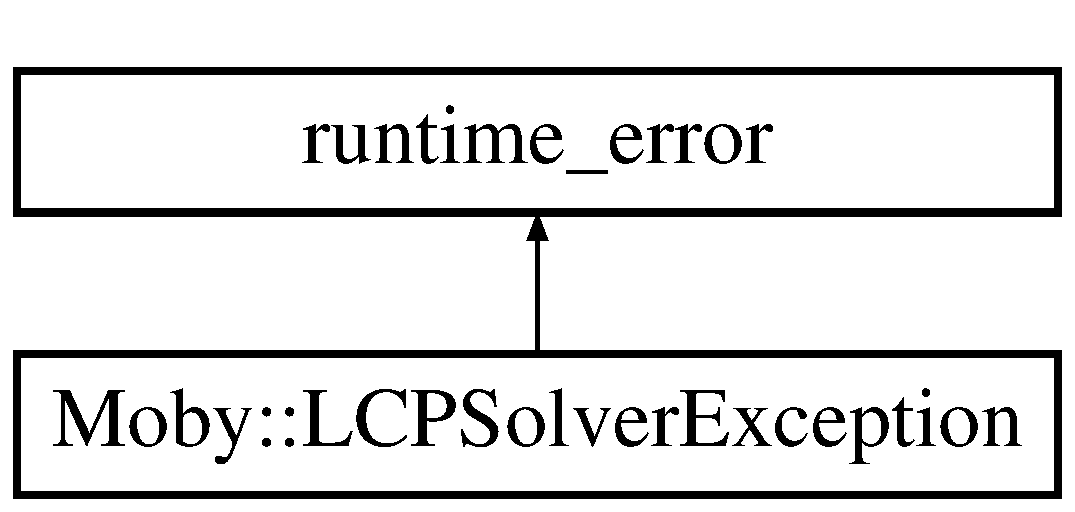
\includegraphics[height=2.000000cm]{classMoby_1_1LCPSolverException}
\end{center}
\end{figure}


\subsection{Detailed Description}
Exception thrown when L\-C\-P solver can't solve. 

The documentation for this class was generated from the following file\-:\begin{DoxyCompactItemize}
\item 
/home/drum/\-Moby/include/\-Moby/L\-C\-P\-Solver\-Exception.\-h\end{DoxyCompactItemize}

\section{Moby\-:\-:Log$<$ Output\-Policy $>$ Class Template Reference}
\label{classMoby_1_1Log}\index{Moby\-::\-Log$<$ Output\-Policy $>$@{Moby\-::\-Log$<$ Output\-Policy $>$}}


\doxyref{Moby}{p.}{namespaceMoby}'s logging utility.  




{\ttfamily \#include $<$Log.\-h$>$}

\subsection*{Public Member Functions}
\begin{DoxyCompactItemize}
\item 
std\-::ostringstream \& {\bfseries get} (unsigned level=0)\label{classMoby_1_1Log_acbee11b723d5f2173e929ff86dbbe90f}

\end{DoxyCompactItemize}
\subsection*{Static Public Attributes}
\begin{DoxyCompactItemize}
\item 
static unsigned {\bfseries reporting\-\_\-level} = 0\label{classMoby_1_1Log_a6848985c90dcce0b86a9d541e32d5770}

\end{DoxyCompactItemize}


\subsection{Detailed Description}
\subsubsection*{template$<$typename Output\-Policy$>$class Moby\-::\-Log$<$ Output\-Policy $>$}

\doxyref{Moby}{p.}{namespaceMoby}'s logging utility. 

The documentation for this class was generated from the following file\-:\begin{DoxyCompactItemize}
\item 
/home/drum/\-Moby/include/\-Moby/Log.\-h\end{DoxyCompactItemize}

\section{Moby\-:\-:Matrix\-Block Struct Reference}
\label{structMoby_1_1MatrixBlock}\index{Moby\-::\-Matrix\-Block@{Moby\-::\-Matrix\-Block}}


Matrix block.  




{\ttfamily \#include $<$Sparse\-Jacobian.\-h$>$}

\subsection*{Public Member Functions}
\begin{DoxyCompactItemize}
\item 
unsigned {\bfseries rows} () const \label{structMoby_1_1MatrixBlock_aea229067d1ba93b738fd900c6b679e09}

\item 
unsigned {\bfseries columns} () const \label{structMoby_1_1MatrixBlock_a9c092dd6dc9708c1653292c81f7e24b5}

\end{DoxyCompactItemize}
\subsection*{Public Attributes}
\begin{DoxyCompactItemize}
\item 
unsigned {\bfseries st\-\_\-col\-\_\-idx}\label{structMoby_1_1MatrixBlock_aa643de96dcb5e1dc098a1c7b31ce90ca}

\item 
unsigned {\bfseries st\-\_\-row\-\_\-idx}\label{structMoby_1_1MatrixBlock_ab2ad71843925ebe0b047e3c66ffad2ad}

\item 
Ravelin\-::\-Matrix\-Nd {\bfseries block}\label{structMoby_1_1MatrixBlock_aa289ae627e4f3be31c60c3cf8bcf0f07}

\end{DoxyCompactItemize}


\subsection{Detailed Description}
Matrix block. 

The block itself is dense and starts at row st\-\_\-row\-\_\-idx and column st\-\_\-col\-\_\-idx of the dense matrix. 

The documentation for this struct was generated from the following file\-:\begin{DoxyCompactItemize}
\item 
/home/drum/\-Moby/include/\-Moby/Sparse\-Jacobian.\-h\end{DoxyCompactItemize}

\section{Moby\-:\-:O\-B\-B Class Reference}
\label{classMoby_1_1OBB}\index{Moby\-::\-O\-B\-B@{Moby\-::\-O\-B\-B}}


An oriented bounding box that optionally allows building an \doxyref{O\-B\-B}{p.}{classMoby_1_1OBB} tree.  




{\ttfamily \#include $<$O\-B\-B.\-h$>$}

Inheritance diagram for Moby\-:\-:O\-B\-B\-:\begin{figure}[H]
\begin{center}
\leavevmode
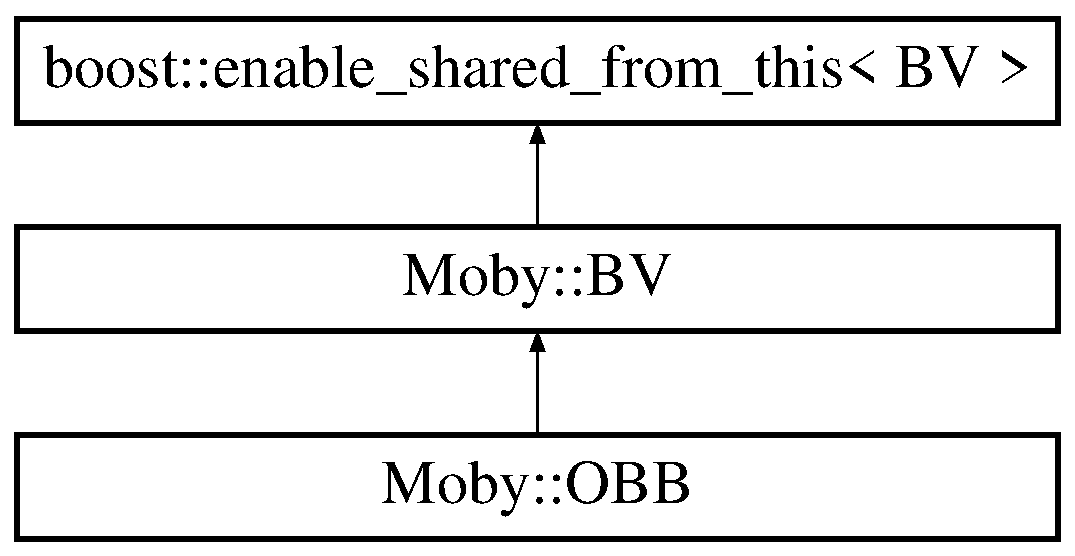
\includegraphics[height=3.000000cm]{classMoby_1_1OBB}
\end{center}
\end{figure}
\subsection*{Public Member Functions}
\begin{DoxyCompactItemize}
\item 
{\bfseries O\-B\-B} (const {\bf O\-B\-B} \&obb)\label{classMoby_1_1OBB_abefec5f3646a09b2bca7df4135ffa21b}

\item 
{\bfseries O\-B\-B} (const {\bf Point3d} \&{\bf center}, const Ravelin\-::\-Matrix3d \&{\bf R}, const Ravelin\-::\-Vector3d \&{\bf l})\label{classMoby_1_1OBB_a709458c4b204c926205f0b77cee09e49}

\item 
{\bfseries O\-B\-B} (const {\bf O\-B\-B} \&o, const Ravelin\-::\-Vector3d \&v)\label{classMoby_1_1OBB_aa41360d0cdb313a5868d69b76ba01fe9}

\item 
{\bf O\-B\-B} \& {\bf operator=} (const {\bf O\-B\-B} \&obb)
\begin{DoxyCompactList}\small\item\em Copies an \doxyref{O\-B\-B}{p.}{classMoby_1_1OBB}. \end{DoxyCompactList}\item 
virtual void {\bf transform} (const Ravelin\-::\-Transform3d \&T, {\bf B\-V} $\ast$result) const \label{classMoby_1_1OBB_a29e0026603c5ab2a421580a40f10e811}

\begin{DoxyCompactList}\small\item\em Transforms the \doxyref{O\-B\-B}{p.}{classMoby_1_1OBB} using the given transform. \end{DoxyCompactList}\item 
virtual {\bf B\-V\-Ptr} {\bf calc\-\_\-swept\-\_\-\-B\-V} ({\bf Collision\-Geometry\-Ptr} g, const Ravelin\-::\-S\-Velocityd \&v) const \label{classMoby_1_1OBB_af319672a637c35433069cc1d84c1288c}

\begin{DoxyCompactList}\small\item\em Calculates the velocity-\/expanded \doxyref{O\-B\-B}{p.}{classMoby_1_1OBB} for a body. \end{DoxyCompactList}\item 
virtual bool {\bf intersects} (const {\bf Line\-Seg3} \&seg, double \&tmin, double tmax, {\bf Point3d} \&q) const \label{classMoby_1_1OBB_a066a51130966a57ce8b09def10431b86}

\begin{DoxyCompactList}\small\item\em Determines whether a line segment intersects the bounding volume. \end{DoxyCompactList}\item 
virtual bool {\bf outside} (const {\bf Point3d} \&point, double tol=N\-E\-A\-R\-\_\-\-Z\-E\-R\-O) const \label{classMoby_1_1OBB_a3450eb0e546b28447917873e4be28916}

\begin{DoxyCompactList}\small\item\em Determines whether a point is outside the bounding volume. \end{DoxyCompactList}\item 
virtual std\-::ostream \& {\bf to\-\_\-vrml} (std\-::ostream \&out, const Ravelin\-::\-Pose3d \&T) const \label{classMoby_1_1OBB_af465225b2600da92a3890d773946f985}

\begin{DoxyCompactList}\small\item\em Outputs the \doxyref{O\-B\-B}{p.}{classMoby_1_1OBB} in V\-R\-M\-L format to the given stream. \end{DoxyCompactList}\item 
unsigned {\bf calc\-\_\-size} () const 
\begin{DoxyCompactList}\small\item\em Constructs an \doxyref{O\-B\-B}{p.}{classMoby_1_1OBB} from a triangle mesh using the mesh inertia method [Ericson, 2003]. \end{DoxyCompactList}\item 
{\bf X\-M\-L\-Tree\-Ptr} {\bf save\-\_\-to\-\_\-xml\-\_\-tree} () const \label{classMoby_1_1OBB_a5a888d661cb639cbd3f59891addb3d68}

\begin{DoxyCompactList}\small\item\em Saves a \doxyref{O\-B\-B}{p.}{classMoby_1_1OBB} hiearchy to a \doxyref{X\-M\-L\-Tree}{p.}{classMoby_1_1XMLTree}. \end{DoxyCompactList}\item 
virtual boost\-::shared\-\_\-ptr\\*
$<$ const Ravelin\-::\-Pose3d $>$ {\bf get\-\_\-relative\-\_\-pose} () const \label{classMoby_1_1OBB_ade3147889bc58cff845dfa73e72650d5}

\begin{DoxyCompactList}\small\item\em Gets the associated pose for this bounding volume. \end{DoxyCompactList}\item 
virtual {\bf Point3d} {\bf get\-\_\-lower\-\_\-bounds} () const \label{classMoby_1_1OBB_ab515ed55a8de4d2d2b5ce79dc051a975}

\begin{DoxyCompactList}\small\item\em Gets the lower bounds on the \doxyref{O\-B\-B}{p.}{classMoby_1_1OBB}. \end{DoxyCompactList}\item 
virtual {\bf Point3d} {\bf get\-\_\-upper\-\_\-bounds} () const \label{classMoby_1_1OBB_a31919685083c0236598c0feb8de48a80}

\begin{DoxyCompactList}\small\item\em Gets the upper bounds on the \doxyref{O\-B\-B}{p.}{classMoby_1_1OBB}. \end{DoxyCompactList}\item 
{\footnotesize template$<$class Forward\-Iterator $>$ }\\void {\bf expand\-\_\-to\-\_\-fit} (Forward\-Iterator begin, Forward\-Iterator end)
\begin{DoxyCompactList}\small\item\em Expands this \doxyref{O\-B\-B}{p.}{classMoby_1_1OBB} (if necessary) to fit the given points. \end{DoxyCompactList}\item 
{\footnotesize template$<$class Forward\-Iterator $>$ }\\{\bf O\-B\-B} (Forward\-Iterator begin, Forward\-Iterator end)
\begin{DoxyCompactList}\small\item\em Computes an \doxyref{O\-B\-B}{p.}{classMoby_1_1OBB} from a set of points. \end{DoxyCompactList}\item 
{\footnotesize template$<$class Output\-Iterator $>$ }\\Output\-Iterator {\bf get\-\_\-vertices} (Output\-Iterator begin) const 
\begin{DoxyCompactList}\small\item\em Gets the eight vertices of the bounding box. \end{DoxyCompactList}\item 
virtual double {\bf calc\-\_\-volume} () const \label{classMoby_1_1OBB_a33ff505f3a3e775c2a43efbea484952b}

\begin{DoxyCompactList}\small\item\em Calculates 1/8th of the volume of the bounding box. \end{DoxyCompactList}\item 
{\footnotesize template$<$class Forward\-Iterator $>$ }\\{\bf O\-B\-B} {\bf calc\-\_\-low\-\_\-dim\-\_\-\-O\-B\-B} (Forward\-Iterator begin, Forward\-Iterator end)
\begin{DoxyCompactList}\small\item\em Computes the minimum \doxyref{O\-B\-B}{p.}{classMoby_1_1OBB} from a set of lower dimensional ($<$ 3d) points. \end{DoxyCompactList}\item 
{\footnotesize template$<$class Forward\-Iterator $>$ }\\{\bf O\-B\-B} {\bf calc\-\_\-min\-\_\-volume\-\_\-\-O\-B\-B} (Forward\-Iterator begin, Forward\-Iterator end)
\begin{DoxyCompactList}\small\item\em Computes the minimum \doxyref{O\-B\-B}{p.}{classMoby_1_1OBB} from a set of points. \end{DoxyCompactList}\item 
{\footnotesize template$<$class Forward\-Iterator $>$ }\\{\bf O\-B\-B} (Forward\-Iterator begin, Forward\-Iterator end)
\begin{DoxyCompactList}\small\item\em Computes an \doxyref{O\-B\-B}{p.}{classMoby_1_1OBB} from a set of points. \end{DoxyCompactList}\item 
{\footnotesize template$<$class Forward\-Iterator $>$ }\\void {\bf expand\-\_\-to\-\_\-fit} (Forward\-Iterator begin, Forward\-Iterator end)
\begin{DoxyCompactList}\small\item\em Expands this \doxyref{O\-B\-B}{p.}{classMoby_1_1OBB} (if necessary) to fit the given points. \end{DoxyCompactList}\item 
{\footnotesize template$<$class Forward\-Iterator $>$ }\\void {\bf align} (Forward\-Iterator begin, Forward\-Iterator end, const Ravelin\-::\-Vector3d \&d1, Ravelin\-::\-Vector3d \&d2)\label{classMoby_1_1OBB_a4cc3a6e9c3d92cd3f2b7b71069b4ccc3}

\begin{DoxyCompactList}\small\item\em Aligns this \doxyref{O\-B\-B}{p.}{classMoby_1_1OBB} with the minimum area bounding rectangle projected along the first dimension of the \doxyref{O\-B\-B}{p.}{classMoby_1_1OBB}. \end{DoxyCompactList}\item 
{\footnotesize template$<$class Output\-Iterator $>$ }\\Output\-Iterator {\bf get\-\_\-vertices} (Output\-Iterator begin) const 
\begin{DoxyCompactList}\small\item\em Gets the eight vertices of the bounding box. \end{DoxyCompactList}\item 
{\footnotesize template$<$class Forward\-Iterator $>$ }\\void {\bfseries calc\-\_\-lengths} (const Ravelin\-::\-Vector3d \&d1, const Ravelin\-::\-Vector3d \&d2, const Ravelin\-::\-Vector3d \&d3, const {\bf Point3d} \&{\bf center}, Forward\-Iterator begin, Forward\-Iterator end, double lengths[3])\label{classMoby_1_1OBB_adca65c7aa27b377bfc2da428eaba9ff8}

\end{DoxyCompactItemize}
\subsection*{Static Public Member Functions}
\begin{DoxyCompactItemize}
\item 
static double {\bf calc\-\_\-sq\-\_\-dist} (const {\bf O\-B\-B} \&o, const {\bf Point3d} \&p)\label{classMoby_1_1OBB_a899812e2c1eac02d0ca19b4fee1d9945}

\begin{DoxyCompactList}\small\item\em Computes the squared distance from a point to an \doxyref{O\-B\-B}{p.}{classMoby_1_1OBB}. \end{DoxyCompactList}\item 
static double {\bf calc\-\_\-dist} (const {\bf O\-B\-B} \&a, const {\bf O\-B\-B} \&b, {\bf Point3d} \&cpa, {\bf Point3d} \&cpb)\label{classMoby_1_1OBB_ad47199249136e149b49e5e31cfe092f2}

\begin{DoxyCompactList}\small\item\em Determines the distance between two O\-B\-Bs. \end{DoxyCompactList}\item 
static double {\bfseries calc\-\_\-dist} (const {\bf O\-B\-B} \&a, const {\bf O\-B\-B} \&b, const Ravelin\-::\-Transform3d \&a\-Tb, {\bf Point3d} \&cpa, {\bf Point3d} \&cpb)\label{classMoby_1_1OBB_abbed0a3a9766ab23beb8cce5cadf40be}

\item 
static bool {\bf intersects} (const {\bf O\-B\-B} \&a, const {\bf O\-B\-B} \&b)
\begin{DoxyCompactList}\small\item\em Determines whether two O\-B\-Bs intersect another. \end{DoxyCompactList}\item 
static bool {\bfseries intersects} (const {\bf O\-B\-B} \&a, const {\bf O\-B\-B} \&b, const Ravelin\-::\-Transform3d \&a\-Tb)\label{classMoby_1_1OBB_abf3fdc71269375625e633ac359c91fdf}

\item 
static bool {\bf intersects} (const {\bf O\-B\-B} \&a, const {\bf Line\-Seg3} \&seg, double \&tmin, double tmax, {\bf Point3d} \&q)
\begin{DoxyCompactList}\small\item\em Determines whether an \doxyref{O\-B\-B}{p.}{classMoby_1_1OBB} and a line/ray/line segment intersect. \end{DoxyCompactList}\item 
static bool {\bf outside} (const {\bf O\-B\-B} \&a, const {\bf Point3d} \&point, double tol=N\-E\-A\-R\-\_\-\-Z\-E\-R\-O)\label{classMoby_1_1OBB_aac6bc5e8a9f05c6a426c6adfededffe7}

\begin{DoxyCompactList}\small\item\em Determines whether a point is outside a \doxyref{O\-B\-B}{p.}{classMoby_1_1OBB} to within the given tolerance. \end{DoxyCompactList}\item 
static {\bf O\-B\-B\-Ptr} {\bf load\-\_\-from\-\_\-xml} (boost\-::shared\-\_\-ptr$<$ const {\bf X\-M\-L\-Tree} $>$ root)\label{classMoby_1_1OBB_ab9b00912d0db0ee09e989b746e4f4924}

\begin{DoxyCompactList}\small\item\em Loads an \doxyref{O\-B\-B}{p.}{classMoby_1_1OBB} hierarchy from a X\-M\-L tree. \end{DoxyCompactList}\item 
{\footnotesize template$<$class Forward\-Iterator $>$ }\\static {\bf O\-B\-B} {\bf calc\-\_\-min\-\_\-volume\-\_\-\-O\-B\-B} (Forward\-Iterator begin, Forward\-Iterator end)
\begin{DoxyCompactList}\small\item\em Computes the minimum \doxyref{O\-B\-B}{p.}{classMoby_1_1OBB} from a set of points. \end{DoxyCompactList}\end{DoxyCompactItemize}
\subsection*{Public Attributes}
\begin{DoxyCompactItemize}
\item 
{\bf Point3d} {\bf center}\label{classMoby_1_1OBB_a2ad27c78cba9efc6a756246373b39120}

\begin{DoxyCompactList}\small\item\em Center of the bounding box. \end{DoxyCompactList}\item 
Ravelin\-::\-Vector3d {\bf l}\label{classMoby_1_1OBB_aedaed5e28878b1af8061960cccbf8fa8}

\begin{DoxyCompactList}\small\item\em Half-\/lengths of the O\-B\-Bs in the three axes directions (i.\-e., in the box frame) \end{DoxyCompactList}\item 
Ravelin\-::\-Matrix3d {\bf R}\label{classMoby_1_1OBB_a13412537178bf91e676be2b96ccbaec7}

\begin{DoxyCompactList}\small\item\em Orientation of this \doxyref{O\-B\-B}{p.}{classMoby_1_1OBB}. \end{DoxyCompactList}\end{DoxyCompactItemize}


\subsection{Detailed Description}
An oriented bounding box that optionally allows building an \doxyref{O\-B\-B}{p.}{classMoby_1_1OBB} tree. 

\begin{DoxyNote}{Note}
the \doxyref{O\-B\-B}{p.}{classMoby_1_1OBB} is generally constructed such that its frame is aligned with that of the underlying rigid body (or collision geometry). Therefore, the center of the \doxyref{O\-B\-B}{p.}{classMoby_1_1OBB} is computed relative to the center-\/of-\/mass of the body (or the center of the geometry). The orientation of the \doxyref{O\-B\-B}{p.}{classMoby_1_1OBB} will always be identical to the orientation of the rigid body (or collision geometry). 
\end{DoxyNote}


\subsection{Constructor \& Destructor Documentation}
\index{Moby\-::\-O\-B\-B@{Moby\-::\-O\-B\-B}!O\-B\-B@{O\-B\-B}}
\index{O\-B\-B@{O\-B\-B}!Moby::OBB@{Moby\-::\-O\-B\-B}}
\subsubsection[{O\-B\-B}]{\setlength{\rightskip}{0pt plus 5cm}template$<$class Forward\-Iterator $>$ Moby\-::\-O\-B\-B\-::\-O\-B\-B (
\begin{DoxyParamCaption}
\item[{Forward\-Iterator}]{begin, }
\item[{Forward\-Iterator}]{end}
\end{DoxyParamCaption}
)}\label{classMoby_1_1OBB_a753abf6baacb9ce0dac16751aaf8fbb1}


Computes an \doxyref{O\-B\-B}{p.}{classMoby_1_1OBB} from a set of points. 


\begin{DoxyParams}{Parameters}
{\em begin} & an iterator to type Point3d \\
\hline
{\em end} & an iterator to type Point3d Algorithm taken from [Ericson, 2005] \\
\hline
\end{DoxyParams}
\index{Moby\-::\-O\-B\-B@{Moby\-::\-O\-B\-B}!O\-B\-B@{O\-B\-B}}
\index{O\-B\-B@{O\-B\-B}!Moby::OBB@{Moby\-::\-O\-B\-B}}
\subsubsection[{O\-B\-B}]{\setlength{\rightskip}{0pt plus 5cm}template$<$class Forward\-Iterator $>$ Moby\-::\-O\-B\-B\-::\-O\-B\-B (
\begin{DoxyParamCaption}
\item[{Forward\-Iterator}]{begin, }
\item[{Forward\-Iterator}]{end}
\end{DoxyParamCaption}
)}\label{classMoby_1_1OBB_a753abf6baacb9ce0dac16751aaf8fbb1}


Computes an \doxyref{O\-B\-B}{p.}{classMoby_1_1OBB} from a set of points. 


\begin{DoxyParams}{Parameters}
{\em begin} & an iterator to type Point3d \\
\hline
{\em end} & an iterator to type Point3d Algorithm taken from [Ericson, 2005] \\
\hline
\end{DoxyParams}


References Moby\-::\-Indexed\-Tri\-::a, Moby\-::\-Indexed\-Tri\-::b, and Moby\-::\-Indexed\-Tri\-::c.



\subsection{Member Function Documentation}
\index{Moby\-::\-O\-B\-B@{Moby\-::\-O\-B\-B}!calc\-\_\-low\-\_\-dim\-\_\-\-O\-B\-B@{calc\-\_\-low\-\_\-dim\-\_\-\-O\-B\-B}}
\index{calc\-\_\-low\-\_\-dim\-\_\-\-O\-B\-B@{calc\-\_\-low\-\_\-dim\-\_\-\-O\-B\-B}!Moby::OBB@{Moby\-::\-O\-B\-B}}
\subsubsection[{calc\-\_\-low\-\_\-dim\-\_\-\-O\-B\-B}]{\setlength{\rightskip}{0pt plus 5cm}template$<$class Forward\-Iterator $>$ {\bf O\-B\-B} Moby\-::\-O\-B\-B\-::calc\-\_\-low\-\_\-dim\-\_\-\-O\-B\-B (
\begin{DoxyParamCaption}
\item[{Forward\-Iterator}]{begin, }
\item[{Forward\-Iterator}]{end}
\end{DoxyParamCaption}
)}\label{classMoby_1_1OBB_ad77112101fc980bc79739d00cfdd163a}


Computes the minimum \doxyref{O\-B\-B}{p.}{classMoby_1_1OBB} from a set of lower dimensional ($<$ 3d) points. 


\begin{DoxyParams}{Parameters}
{\em begin} & an iterator to type Point3d \\
\hline
{\em end} & an iterator to type Point3d \\
\hline
\end{DoxyParams}


References center, l, and R.

\index{Moby\-::\-O\-B\-B@{Moby\-::\-O\-B\-B}!calc\-\_\-min\-\_\-volume\-\_\-\-O\-B\-B@{calc\-\_\-min\-\_\-volume\-\_\-\-O\-B\-B}}
\index{calc\-\_\-min\-\_\-volume\-\_\-\-O\-B\-B@{calc\-\_\-min\-\_\-volume\-\_\-\-O\-B\-B}!Moby::OBB@{Moby\-::\-O\-B\-B}}
\subsubsection[{calc\-\_\-min\-\_\-volume\-\_\-\-O\-B\-B}]{\setlength{\rightskip}{0pt plus 5cm}template$<$class Forward\-Iterator $>$ {\bf O\-B\-B} Moby\-::\-O\-B\-B\-::calc\-\_\-min\-\_\-volume\-\_\-\-O\-B\-B (
\begin{DoxyParamCaption}
\item[{Forward\-Iterator}]{begin, }
\item[{Forward\-Iterator}]{end}
\end{DoxyParamCaption}
)\hspace{0.3cm}{\ttfamily [static]}}\label{classMoby_1_1OBB_aa0c199492e8198f4c3a321d3da8bc5d3}


Computes the minimum \doxyref{O\-B\-B}{p.}{classMoby_1_1OBB} from a set of points. 


\begin{DoxyParams}{Parameters}
{\em begin} & an iterator to type Point3d \\
\hline
{\em end} & an iterator to type Point3d Algorithm taken from {\tt http\-://www.\-geometrictools.\-com} -\/ thanks Dave Eberly! \\
\hline
\end{DoxyParams}
\index{Moby\-::\-O\-B\-B@{Moby\-::\-O\-B\-B}!calc\-\_\-min\-\_\-volume\-\_\-\-O\-B\-B@{calc\-\_\-min\-\_\-volume\-\_\-\-O\-B\-B}}
\index{calc\-\_\-min\-\_\-volume\-\_\-\-O\-B\-B@{calc\-\_\-min\-\_\-volume\-\_\-\-O\-B\-B}!Moby::OBB@{Moby\-::\-O\-B\-B}}
\subsubsection[{calc\-\_\-min\-\_\-volume\-\_\-\-O\-B\-B}]{\setlength{\rightskip}{0pt plus 5cm}template$<$class Forward\-Iterator $>$ {\bf O\-B\-B} Moby\-::\-O\-B\-B\-::calc\-\_\-min\-\_\-volume\-\_\-\-O\-B\-B (
\begin{DoxyParamCaption}
\item[{Forward\-Iterator}]{begin, }
\item[{Forward\-Iterator}]{end}
\end{DoxyParamCaption}
)}\label{classMoby_1_1OBB_aa0c199492e8198f4c3a321d3da8bc5d3}


Computes the minimum \doxyref{O\-B\-B}{p.}{classMoby_1_1OBB} from a set of points. 


\begin{DoxyParams}{Parameters}
{\em begin} & an iterator to type Point3d \\
\hline
{\em end} & an iterator to type Point3d Algorithm taken from {\tt http\-://www.\-geometrictools.\-com} -\/ thanks Dave Eberly! \\
\hline
\end{DoxyParams}


References calc\-\_\-volume(), center, Moby\-::\-Indexed\-Tri\-Array\-::determine\-\_\-edge\-\_\-facet\-\_\-map(), Moby\-::\-Indexed\-Tri\-Array\-::determine\-\_\-vertex\-\_\-edge\-\_\-map(), Moby\-::\-Indexed\-Tri\-Array\-::get\-\_\-triangle(), Moby\-::\-Indexed\-Tri\-Array\-::get\-\_\-vertices(), Moby\-::\-Indexed\-Tri\-Array\-::is\-\_\-coplanar(), l, and R.

\index{Moby\-::\-O\-B\-B@{Moby\-::\-O\-B\-B}!calc\-\_\-size@{calc\-\_\-size}}
\index{calc\-\_\-size@{calc\-\_\-size}!Moby::OBB@{Moby\-::\-O\-B\-B}}
\subsubsection[{calc\-\_\-size}]{\setlength{\rightskip}{0pt plus 5cm}unsigned O\-B\-B\-::calc\-\_\-size (
\begin{DoxyParamCaption}
{}
\end{DoxyParamCaption}
) const}\label{classMoby_1_1OBB_a77342d5b6ba7350ca765da4bc489827a}


Constructs an \doxyref{O\-B\-B}{p.}{classMoby_1_1OBB} from a triangle mesh using the mesh inertia method [Ericson, 2003]. 

Requires a O(n) operation to compute the inertial properties of the triangle mesh\-Calculates the size (number of elements in) of an \doxyref{O\-B\-B}{p.}{classMoby_1_1OBB} tree \index{Moby\-::\-O\-B\-B@{Moby\-::\-O\-B\-B}!expand\-\_\-to\-\_\-fit@{expand\-\_\-to\-\_\-fit}}
\index{expand\-\_\-to\-\_\-fit@{expand\-\_\-to\-\_\-fit}!Moby::OBB@{Moby\-::\-O\-B\-B}}
\subsubsection[{expand\-\_\-to\-\_\-fit}]{\setlength{\rightskip}{0pt plus 5cm}template$<$class Forward\-Iterator $>$ void Moby\-::\-O\-B\-B\-::expand\-\_\-to\-\_\-fit (
\begin{DoxyParamCaption}
\item[{Forward\-Iterator}]{begin, }
\item[{Forward\-Iterator}]{end}
\end{DoxyParamCaption}
)}\label{classMoby_1_1OBB_a683af13d508d7f0a34d74d8e9ef3420f}


Expands this \doxyref{O\-B\-B}{p.}{classMoby_1_1OBB} (if necessary) to fit the given points. 


\begin{DoxyParams}{Parameters}
{\em begin} & an iterator to the beginning of a container of type Ravelin\-:\-Point3d\-: \\
\hline
{\em end} & an iterator to the end of a container of type Point3d \\
\hline
\end{DoxyParams}
\index{Moby\-::\-O\-B\-B@{Moby\-::\-O\-B\-B}!expand\-\_\-to\-\_\-fit@{expand\-\_\-to\-\_\-fit}}
\index{expand\-\_\-to\-\_\-fit@{expand\-\_\-to\-\_\-fit}!Moby::OBB@{Moby\-::\-O\-B\-B}}
\subsubsection[{expand\-\_\-to\-\_\-fit}]{\setlength{\rightskip}{0pt plus 5cm}template$<$class Forward\-Iterator $>$ void Moby\-::\-O\-B\-B\-::expand\-\_\-to\-\_\-fit (
\begin{DoxyParamCaption}
\item[{Forward\-Iterator}]{begin, }
\item[{Forward\-Iterator}]{end}
\end{DoxyParamCaption}
)}\label{classMoby_1_1OBB_a683af13d508d7f0a34d74d8e9ef3420f}


Expands this \doxyref{O\-B\-B}{p.}{classMoby_1_1OBB} (if necessary) to fit the given points. 


\begin{DoxyParams}{Parameters}
{\em begin} & an iterator to the beginning of a container of type Ravelin\-:\-Point3d\-: \\
\hline
{\em end} & an iterator to the end of a container of type Point3d \\
\hline
\end{DoxyParams}
\index{Moby\-::\-O\-B\-B@{Moby\-::\-O\-B\-B}!get\-\_\-vertices@{get\-\_\-vertices}}
\index{get\-\_\-vertices@{get\-\_\-vertices}!Moby::OBB@{Moby\-::\-O\-B\-B}}
\subsubsection[{get\-\_\-vertices}]{\setlength{\rightskip}{0pt plus 5cm}template$<$class Output\-Iterator $>$ Output\-Iterator Moby\-::\-O\-B\-B\-::get\-\_\-vertices (
\begin{DoxyParamCaption}
\item[{Output\-Iterator}]{begin}
\end{DoxyParamCaption}
) const}\label{classMoby_1_1OBB_a8407723ec562bdedceb065a57ada6059}


Gets the eight vertices of the bounding box. 

\begin{DoxyNote}{Note}
vertices are output in no particular order 
\end{DoxyNote}
\index{Moby\-::\-O\-B\-B@{Moby\-::\-O\-B\-B}!get\-\_\-vertices@{get\-\_\-vertices}}
\index{get\-\_\-vertices@{get\-\_\-vertices}!Moby::OBB@{Moby\-::\-O\-B\-B}}
\subsubsection[{get\-\_\-vertices}]{\setlength{\rightskip}{0pt plus 5cm}template$<$class Output\-Iterator $>$ Output\-Iterator Moby\-::\-O\-B\-B\-::get\-\_\-vertices (
\begin{DoxyParamCaption}
\item[{Output\-Iterator}]{begin}
\end{DoxyParamCaption}
) const}\label{classMoby_1_1OBB_a8407723ec562bdedceb065a57ada6059}


Gets the eight vertices of the bounding box. 

\begin{DoxyNote}{Note}
vertices are output in no particular order 
\end{DoxyNote}
\index{Moby\-::\-O\-B\-B@{Moby\-::\-O\-B\-B}!intersects@{intersects}}
\index{intersects@{intersects}!Moby::OBB@{Moby\-::\-O\-B\-B}}
\subsubsection[{intersects}]{\setlength{\rightskip}{0pt plus 5cm}bool O\-B\-B\-::intersects (
\begin{DoxyParamCaption}
\item[{const {\bf O\-B\-B} \&}]{a, }
\item[{const {\bf O\-B\-B} \&}]{b}
\end{DoxyParamCaption}
)\hspace{0.3cm}{\ttfamily [static]}}\label{classMoby_1_1OBB_ab49f1da0e75866cc05a24ea20eca69ae}


Determines whether two O\-B\-Bs intersect another. 

Code adapted from [Ericson, 2005] 

References get\-\_\-relative\-\_\-pose().



Referenced by intersects().

\index{Moby\-::\-O\-B\-B@{Moby\-::\-O\-B\-B}!intersects@{intersects}}
\index{intersects@{intersects}!Moby::OBB@{Moby\-::\-O\-B\-B}}
\subsubsection[{intersects}]{\setlength{\rightskip}{0pt plus 5cm}bool O\-B\-B\-::intersects (
\begin{DoxyParamCaption}
\item[{const {\bf O\-B\-B} \&}]{a, }
\item[{const {\bf Line\-Seg3} \&}]{seg, }
\item[{double \&}]{tmin, }
\item[{double}]{tmax, }
\item[{{\bf Point3d} \&}]{q}
\end{DoxyParamCaption}
)\hspace{0.3cm}{\ttfamily [static]}}\label{classMoby_1_1OBB_aa2d13175c15026999a37fb61487e31a0}


Determines whether an \doxyref{O\-B\-B}{p.}{classMoby_1_1OBB} and a line/ray/line segment intersect. 

When intersecting, return intersection distance tmin and point q of intersection. 
\begin{DoxyParams}{Parameters}
{\em a} & the \doxyref{O\-B\-B}{p.}{classMoby_1_1OBB} to check for intersection \\
\hline
{\em seg} & the line segment to check for intersection \\
\hline
{\em tmin} & on entry, contains the minimum value of the line parameter-\/ for a line segment, this will generally be 0; when an intersection occurs, this will contain the distance of intersection from the tmin that was input on return \\
\hline
{\em tmax} & the maximum value of the line parameter-\/ for a line segment, this will generally be 1 \\
\hline
{\em q} & contains the point of intersection, if any, on return \\
\hline
\end{DoxyParams}
\begin{DoxyReturn}{Returns}
{\bfseries true} if the \doxyref{O\-B\-B}{p.}{classMoby_1_1OBB} and line intersect, {\bfseries false} otherwise 
\end{DoxyReturn}
\begin{DoxyNote}{Note}
code adapted from [Ericson, 2005], pp. 180-\/181 
\end{DoxyNote}


References center, get\-\_\-relative\-\_\-pose(), and R.

\index{Moby\-::\-O\-B\-B@{Moby\-::\-O\-B\-B}!operator=@{operator=}}
\index{operator=@{operator=}!Moby::OBB@{Moby\-::\-O\-B\-B}}
\subsubsection[{operator=}]{\setlength{\rightskip}{0pt plus 5cm}{\bf O\-B\-B} \& O\-B\-B\-::operator= (
\begin{DoxyParamCaption}
\item[{const {\bf O\-B\-B} \&}]{obb}
\end{DoxyParamCaption}
)}\label{classMoby_1_1OBB_a62679c416b02e7e255395a517f5ade7d}


Copies an \doxyref{O\-B\-B}{p.}{classMoby_1_1OBB}. 

\begin{DoxyNote}{Note}
userdata and node info (children) are not copied 
\end{DoxyNote}


References center, Moby\-::\-B\-V\-::geom, l, and R.



The documentation for this class was generated from the following files\-:\begin{DoxyCompactItemize}
\item 
/home/drum/\-Moby/include/\-Moby/O\-B\-B.\-h\item 
/home/drum/\-Moby/include/\-Moby/O\-B\-B.\-inl\item 
/home/drum/\-Moby/src/O\-B\-B.\-cpp\end{DoxyCompactItemize}

\section{Moby\-:\-:O\-S\-G\-Group\-Wrapper Class Reference}
\label{classMoby_1_1OSGGroupWrapper}\index{Moby\-::\-O\-S\-G\-Group\-Wrapper@{Moby\-::\-O\-S\-G\-Group\-Wrapper}}


A wrapper for Open\-Inventor O\-S\-G\-Group class, supporting serialization.  




{\ttfamily \#include $<$O\-S\-G\-Group\-Wrapper.\-h$>$}

Inheritance diagram for Moby\-:\-:O\-S\-G\-Group\-Wrapper\-:\begin{figure}[H]
\begin{center}
\leavevmode
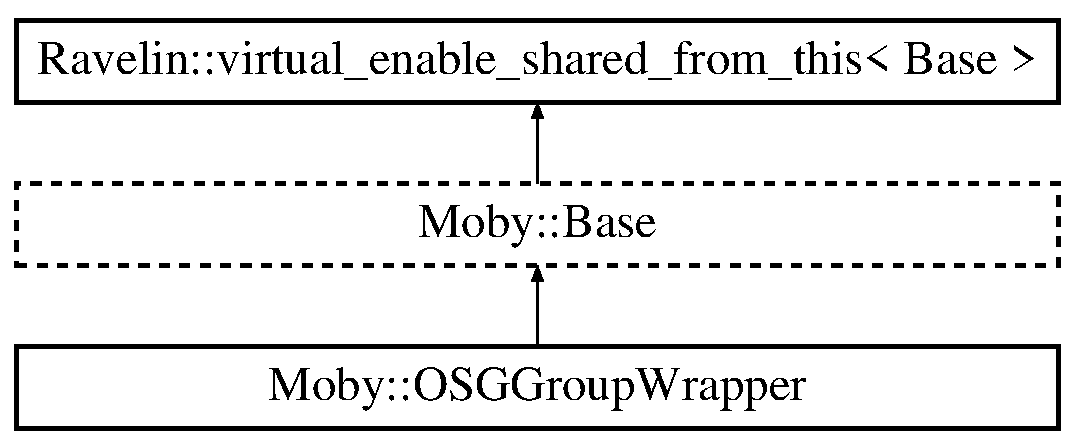
\includegraphics[height=3.000000cm]{classMoby_1_1OSGGroupWrapper}
\end{center}
\end{figure}
\subsection*{Public Member Functions}
\begin{DoxyCompactItemize}
\item 
{\bfseries O\-S\-G\-Group\-Wrapper} (osg\-::\-Node $\ast$n)\label{classMoby_1_1OSGGroupWrapper_a94c0e71c82f79a7bb5cfc1affafe25f4}

\item 
{\bf O\-S\-G\-Group\-Wrapper} (const std\-::string \&filename)\label{classMoby_1_1OSGGroupWrapper_a5d19d8ae45fc443c4a5a02824937ef55}

\begin{DoxyCompactList}\small\item\em Creates an O\-S\-G\-Group wrapper given a filename. \end{DoxyCompactList}\item 
virtual void {\bf load\-\_\-from\-\_\-xml} (boost\-::shared\-\_\-ptr$<$ const {\bf X\-M\-L\-Tree} $>$ node, std\-::map$<$ std\-::string, {\bf Base\-Ptr} $>$ \&id\-\_\-map)\label{classMoby_1_1OSGGroupWrapper_a9d5827d7a78065b9bc376d90e0bac2f9}

\begin{DoxyCompactList}\small\item\em Implements \doxyref{Base\-::load\-\_\-from\-\_\-xml()}{p.}{classMoby_1_1Base_a98b861c1d615a748b576aa613f17389f} \end{DoxyCompactList}\item 
virtual void {\bf save\-\_\-to\-\_\-xml} ({\bf X\-M\-L\-Tree\-Ptr} node, std\-::list$<$ boost\-::shared\-\_\-ptr$<$ const {\bf Base} $>$ $>$ \&shared\-\_\-objects) const \label{classMoby_1_1OSGGroupWrapper_ae407d4e31677c2516bd5ed795de535f7}

\begin{DoxyCompactList}\small\item\em Implements \doxyref{Base\-::save\-\_\-to\-\_\-xml()}{p.}{classMoby_1_1Base_aed64905ca39893d02d1e6c3f03f73aa9} \end{DoxyCompactList}\item 
osg\-::\-Group $\ast$ {\bfseries get\-\_\-group} ()\label{classMoby_1_1OSGGroupWrapper_a0398989589343df6e3f33b8e1919dde8}

\end{DoxyCompactItemize}
\subsection*{Additional Inherited Members}


\subsection{Detailed Description}
A wrapper for Open\-Inventor O\-S\-G\-Group class, supporting serialization. 

The documentation for this class was generated from the following files\-:\begin{DoxyCompactItemize}
\item 
/home/drum/\-Moby/include/\-Moby/O\-S\-G\-Group\-Wrapper.\-h\item 
/home/drum/\-Moby/src/O\-S\-G\-Group\-Wrapper.\-cpp\end{DoxyCompactItemize}

\section{osg\-:\-:Osg\-Torus Class Reference}
\label{classosg_1_1OsgTorus}\index{osg\-::\-Osg\-Torus@{osg\-::\-Osg\-Torus}}
\subsection*{Public Member Functions}
\begin{DoxyCompactItemize}
\item 
{\bfseries Osg\-Torus} (float inner, float outer, float start\-\_\-angle=0.\-0f, float end\-\_\-angle=360.\-0f, unsigned int cross=50, unsigned int sweep=50)\label{classosg_1_1OsgTorus_a1cdee09d1a089d8ee6e1fa8d2209f259}

\item 
{\bfseries Osg\-Torus} (const {\bf Osg\-Torus} \&torus)\label{classosg_1_1OsgTorus_a2a3338b9d7fcc1360aea800384bf577d}

\item 
bool {\bfseries valid} () const \label{classosg_1_1OsgTorus_afdacac9241e1c4a404e57e8e70286a48}

\item 
void {\bfseries set} (float i, float o)\label{classosg_1_1OsgTorus_a3f7956c72d7942eb1b0981bae40c8e6b}

\item 
osg\-::\-Geode $\ast$ {\bfseries operator()} () const \label{classosg_1_1OsgTorus_a3bba248565198907dae7d96a54e8159a}

\item 
void {\bfseries set\-Color} (const osg\-::\-Vec4 \&c)\label{classosg_1_1OsgTorus_a47b24fe31f43d4a4a1750e346cc612fb}

\item 
const osg\-::\-Vec4 \& {\bfseries get\-Color} () const \label{classosg_1_1OsgTorus_aef2c9183f791ceaf0b1c5e66aa756b17}

\item 
void {\bfseries set\-Major\-Radius} (float inner)\label{classosg_1_1OsgTorus_a2dd54eb69fec958fddbcb23ceabc26a1}

\item 
float {\bfseries get\-Major\-Radius} () const \label{classosg_1_1OsgTorus_aa2201bb7be1b26215ae1331d6bd88071}

\item 
void {\bfseries set\-Minor\-Radius} (float outer)\label{classosg_1_1OsgTorus_a14a4432d6d107c8a6c08a5c6a701fe73}

\item 
float {\bfseries get\-Minor\-Radius} () const \label{classosg_1_1OsgTorus_ab83c02747957a245f17c4e5756f18054}

\item 
void {\bfseries set\-Start\-Sweep} (float angle)\label{classosg_1_1OsgTorus_afbd60e210e8a88464e505cf63cdb31ce}

\item 
float {\bfseries get\-Start\-Sweep} () const \label{classosg_1_1OsgTorus_ae2c0e6f29f8b36caeea5553149ff0d9b}

\item 
void {\bfseries set\-End\-Sweep} (float angle)\label{classosg_1_1OsgTorus_a8116e35bd3dcedc8cc021c5396ea1136}

\item 
float {\bfseries get\-End\-Sweep} () const \label{classosg_1_1OsgTorus_a0ff2ee8495ea4f9c8d42362430d746a6}

\item 
void {\bfseries set\-Circle\-Cuts} (int cuts)\label{classosg_1_1OsgTorus_a1f587ce2a5d8afa4b0ce0769219d21a4}

\item 
int {\bfseries get\-Circle\-Cuts} () const \label{classosg_1_1OsgTorus_a3df2d359cdb61a6fe8be7a2e759a6c10}

\item 
void {\bfseries set\-Sweep\-Cuts} (int cuts)\label{classosg_1_1OsgTorus_af3a98ebc372399393131d42d7d82c25b}

\item 
int {\bfseries get\-Sweep\-Cuts} () const \label{classosg_1_1OsgTorus_ad46769d293629f45cab343c3ca62e4bc}

\end{DoxyCompactItemize}


The documentation for this class was generated from the following files\-:\begin{DoxyCompactItemize}
\item 
/home/drum/\-Moby/src/Osg\-Torus.\-h\item 
/home/drum/\-Moby/src/Osg\-Torus.\-cpp\end{DoxyCompactItemize}

\section{Moby\-:\-:Output\-To\-File Struct Reference}
\label{structMoby_1_1OutputToFile}\index{Moby\-::\-Output\-To\-File@{Moby\-::\-Output\-To\-File}}
\subsection*{Static Public Member Functions}
\begin{DoxyCompactItemize}
\item 
static void {\bfseries output} (const std\-::string \&msg)\label{structMoby_1_1OutputToFile_a44c6bba677a52dfe1214b04f96c85814}

\end{DoxyCompactItemize}
\subsection*{Static Public Attributes}
\begin{DoxyCompactItemize}
\item 
static std\-::ofstream {\bfseries stream}\label{structMoby_1_1OutputToFile_a74e58c5a617461375ce7e4fadabdf839}

\end{DoxyCompactItemize}


The documentation for this struct was generated from the following files\-:\begin{DoxyCompactItemize}
\item 
/home/drum/\-Moby/include/\-Moby/Log.\-h\item 
/home/drum/\-Moby/src/Log.\-cpp\end{DoxyCompactItemize}

\section{Moby\-:\-:Pairwise\-Dist\-Info Struct Reference}
\label{structMoby_1_1PairwiseDistInfo}\index{Moby\-::\-Pairwise\-Dist\-Info@{Moby\-::\-Pairwise\-Dist\-Info}}


Structure for storing the pairwise distance between pointers to two \doxyref{Collision\-Geometry}{p.}{classMoby_1_1CollisionGeometry} objects.  




{\ttfamily \#include $<$Pairwise\-Dist\-Info.\-h$>$}

\subsection*{Public Attributes}
\begin{DoxyCompactItemize}
\item 
{\bf Collision\-Geometry\-Ptr} {\bfseries a}\label{structMoby_1_1PairwiseDistInfo_a8fe6b87866eb8addd1fb07655a4851a5}

\item 
{\bf Collision\-Geometry\-Ptr} {\bfseries b}\label{structMoby_1_1PairwiseDistInfo_a466fd3b1374a0d486703cc3b7e76dd5a}

\item 
double {\bfseries dist}\label{structMoby_1_1PairwiseDistInfo_a08ab895e839297f4944dd99f854e04e2}

\item 
{\bf Point3d} {\bfseries pa}\label{structMoby_1_1PairwiseDistInfo_a6bc86c2db72fc677df5c97109269be87}

\item 
{\bf Point3d} {\bfseries pb}\label{structMoby_1_1PairwiseDistInfo_a8f71e9e4378c4d56990888a9792cd682}

\end{DoxyCompactItemize}


\subsection{Detailed Description}
Structure for storing the pairwise distance between pointers to two \doxyref{Collision\-Geometry}{p.}{classMoby_1_1CollisionGeometry} objects. 

The documentation for this struct was generated from the following file\-:\begin{DoxyCompactItemize}
\item 
/home/drum/\-Moby/include/\-Moby/Pairwise\-Dist\-Info.\-h\end{DoxyCompactItemize}

\section{Moby\-:\-:Penalty\-Constraint\-Handler Class Reference}
\label{classMoby_1_1PenaltyConstraintHandler}\index{Moby\-::\-Penalty\-Constraint\-Handler@{Moby\-::\-Penalty\-Constraint\-Handler}}


Defines the mechanism for handling Penalty constraints.  




{\ttfamily \#include $<$Penalty\-Constraint\-Handler.\-h$>$}

\subsection*{Public Member Functions}
\begin{DoxyCompactItemize}
\item 
{\bf Penalty\-Constraint\-Handler} ()\label{classMoby_1_1PenaltyConstraintHandler_a3be02bf3562a8432b0cd020f39aae026}

\begin{DoxyCompactList}\small\item\em Sets up the default parameters for the Penalty constraint handler. \end{DoxyCompactList}\item 
void {\bfseries process\-\_\-constraints} (const std\-::vector$<$ {\bf Unilateral\-Constraint} $>$ \&constraints) const \label{classMoby_1_1PenaltyConstraintHandler_a779dba3e53057f3a824c63ba4f3564e1}

\end{DoxyCompactItemize}


\subsection{Detailed Description}
Defines the mechanism for handling Penalty constraints. 

The documentation for this class was generated from the following files\-:\begin{DoxyCompactItemize}
\item 
/home/drum/\-Moby/include/\-Moby/Penalty\-Constraint\-Handler.\-h\item 
/home/drum/\-Moby/src/Penalty\-Constraint\-Handler.\-cpp\end{DoxyCompactItemize}

\section{Moby\-:\-:Planar\-Joint Class Reference}
\label{classMoby_1_1PlanarJoint}\index{Moby\-::\-Planar\-Joint@{Moby\-::\-Planar\-Joint}}


Defines an actuated spherical joint.  




{\ttfamily \#include $<$Planar\-Joint.\-h$>$}

Inheritance diagram for Moby\-:\-:Planar\-Joint\-:\begin{figure}[H]
\begin{center}
\leavevmode
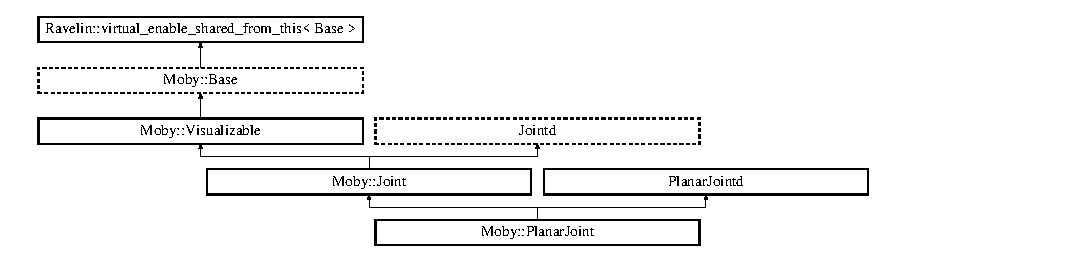
\includegraphics[height=3.070176cm]{classMoby_1_1PlanarJoint}
\end{center}
\end{figure}
\subsection*{Public Member Functions}
\begin{DoxyCompactItemize}
\item 
{\bf Planar\-Joint} ()
\begin{DoxyCompactList}\small\item\em Initializes the joint. \end{DoxyCompactList}\item 
{\bf Planar\-Joint} (boost\-::weak\-\_\-ptr$<$ {\bf Rigid\-Body} $>$ inboard, boost\-::weak\-\_\-ptr$<$ {\bf Rigid\-Body} $>$ outboard)
\begin{DoxyCompactList}\small\item\em Initializes the joint with the specified inboard and outboard links. \end{DoxyCompactList}\item 
virtual unsigned {\bfseries num\-\_\-dof} () const \label{classMoby_1_1PlanarJoint_a0933a67e787a8c1510551356ea62e7c5}

\item 
virtual bool {\bfseries is\-\_\-singular\-\_\-config} () const \label{classMoby_1_1PlanarJoint_a3cd2bfbd203ee41b8d093f3950853932}

\item 
virtual void {\bfseries evaluate\-\_\-constraints} (double C[$\,$])\label{classMoby_1_1PlanarJoint_ab4a4b8a9235c71c9cb228280a877338c}

\item 
virtual const std\-::vector\\*
$<$ Ravelin\-::\-S\-Velocityd $>$ \& {\bfseries get\-\_\-spatial\-\_\-axes\-\_\-dot} ()\label{classMoby_1_1PlanarJoint_adc7a0dee7253ed2fd4cbeff9cff37b6c}

\item 
virtual void {\bfseries determine\-\_\-q} (Ravelin\-::\-Vector\-Nd \&q)\label{classMoby_1_1PlanarJoint_acc0879d3f08a40b05beaf915dad07d5c}

\item 
virtual boost\-::shared\-\_\-ptr\\*
$<$ const Ravelin\-::\-Pose3d $>$ {\bfseries get\-\_\-induced\-\_\-pose} ()\label{classMoby_1_1PlanarJoint_ab9c9a213d0296de995f0ebe822aad527}

\item 
virtual void {\bf load\-\_\-from\-\_\-xml} (boost\-::shared\-\_\-ptr$<$ const {\bf X\-M\-L\-Tree} $>$ node, std\-::map$<$ std\-::string, {\bf Base\-Ptr} $>$ \&id\-\_\-map)\label{classMoby_1_1PlanarJoint_abc73fa718eff71b90bbd0ce4ba92106d}

\begin{DoxyCompactList}\small\item\em Implements \doxyref{Base\-::load\-\_\-from\-\_\-xml()}{p.}{classMoby_1_1Base_a98b861c1d615a748b576aa613f17389f} \end{DoxyCompactList}\item 
virtual void {\bf save\-\_\-to\-\_\-xml} ({\bf X\-M\-L\-Tree\-Ptr} node, std\-::list$<$ boost\-::shared\-\_\-ptr$<$ const {\bf Base} $>$ $>$ \&shared\-\_\-objects) const \label{classMoby_1_1PlanarJoint_a3614b2d0ff84262b8eb3656320e484a1}

\begin{DoxyCompactList}\small\item\em Implements \doxyref{Base\-::save\-\_\-to\-\_\-xml()}{p.}{classMoby_1_1Base_aed64905ca39893d02d1e6c3f03f73aa9} \end{DoxyCompactList}\end{DoxyCompactItemize}
\subsection*{Additional Inherited Members}


\subsection{Detailed Description}
Defines an actuated spherical joint. 

\subsection{Constructor \& Destructor Documentation}
\index{Moby\-::\-Planar\-Joint@{Moby\-::\-Planar\-Joint}!Planar\-Joint@{Planar\-Joint}}
\index{Planar\-Joint@{Planar\-Joint}!Moby::PlanarJoint@{Moby\-::\-Planar\-Joint}}
\subsubsection[{Planar\-Joint}]{\setlength{\rightskip}{0pt plus 5cm}Planar\-Joint\-::\-Planar\-Joint (
\begin{DoxyParamCaption}
{}
\end{DoxyParamCaption}
)}\label{classMoby_1_1PlanarJoint_a97e2084bce8d998d891aac3f281f70ca}


Initializes the joint. 

The axes of rotation are each set to [0 0 0]. The inboard and outboard links are set to N\-U\-L\-L. 

References Moby\-::\-Joint\-::init\-\_\-data().

\index{Moby\-::\-Planar\-Joint@{Moby\-::\-Planar\-Joint}!Planar\-Joint@{Planar\-Joint}}
\index{Planar\-Joint@{Planar\-Joint}!Moby::PlanarJoint@{Moby\-::\-Planar\-Joint}}
\subsubsection[{Planar\-Joint}]{\setlength{\rightskip}{0pt plus 5cm}Planar\-Joint\-::\-Planar\-Joint (
\begin{DoxyParamCaption}
\item[{boost\-::weak\-\_\-ptr$<$ {\bf Rigid\-Body} $>$}]{inboard, }
\item[{boost\-::weak\-\_\-ptr$<$ {\bf Rigid\-Body} $>$}]{outboard}
\end{DoxyParamCaption}
)}\label{classMoby_1_1PlanarJoint_a24b1e7f2b4317f4a91b020bed31abbde}


Initializes the joint with the specified inboard and outboard links. 

The axis of rotation is set to [0 0 0]. 

The documentation for this class was generated from the following files\-:\begin{DoxyCompactItemize}
\item 
/home/drum/\-Moby/include/\-Moby/Planar\-Joint.\-h\item 
/home/drum/\-Moby/src/Planar\-Joint.\-cpp\end{DoxyCompactItemize}

\section{Moby\-:\-:Plane Class Reference}
\label{classMoby_1_1Plane}\index{Moby\-::\-Plane@{Moby\-::\-Plane}}


Defines a plane using the equation $<$n, x$>$ = d.  




{\ttfamily \#include $<$Plane.\-h$>$}

\subsection*{Public Member Functions}
\begin{DoxyCompactItemize}
\item 
{\bfseries Plane} (double nx, double ny, double nz, double d)\label{classMoby_1_1Plane_a37d5c13a0133d6c55eee5af96e16575b}

\item 
{\bfseries Plane} (const Triangle \&t)\label{classMoby_1_1Plane_ab4803d0bc581e56d2f5cf9c48e2a2044}

\item 
{\bfseries Plane} (const Ravelin\-::\-Vector3d \&n, double d)\label{classMoby_1_1Plane_a84f280d1d73658bf227357c6940797a9}

\item 
{\bfseries Plane} (const Ravelin\-::\-Vector3d \&normal, const {\bf Point3d} \&point)\label{classMoby_1_1Plane_a71722c6521f295bddf1d1924f43b0f30}

\item 
{\bfseries Plane} (const {\bf Plane} \&p)\label{classMoby_1_1Plane_a48ac08a469ed2e23012e155780bb4551}

\item 
void {\bfseries operator=} (const {\bf Plane} \&p)\label{classMoby_1_1Plane_a799034ea4bec6820f37e73fd43adad00}

\item 
double {\bfseries calc\-\_\-signed\-\_\-distance} (const {\bf Point3d} \&p) const \label{classMoby_1_1Plane_ab81f0d7cd2d017bd67424575135201b2}

\item 
bool {\bfseries on\-\_\-plane} (const {\bf Point3d} \&p)\label{classMoby_1_1Plane_a995274cd185b194bf5b9a951a2e41755}

\item 
bool {\bfseries operator==} (const {\bf Plane} \&p) const \label{classMoby_1_1Plane_a1286cb4e4ce40ec860a7a8323331286f}

\item 
bool {\bfseries operator$<$} (const {\bf Plane} \&p) const \label{classMoby_1_1Plane_ae09c64e9d1b9932a983f374ce6daaf61}

\item 
boost\-::shared\-\_\-ptr$<$ const \\*
Ravelin\-::\-Pose3d $>$ {\bfseries get\-\_\-pose} () const \label{classMoby_1_1Plane_ab84e59e12388876e8633d6a015b0e134}

\item 
{\bf Point3d} {\bf project} (const {\bf Point3d} \&p) const \label{classMoby_1_1Plane_ad111c206860bc0686214e63e76b992f7}

\begin{DoxyCompactList}\small\item\em Projects a point onto the plane. \end{DoxyCompactList}\item 
Ravelin\-::\-Origin2d {\bf to\-\_\-2\-D} (const {\bf Point3d} \&p) const \label{classMoby_1_1Plane_a0e3d453d95102cbe683cd2e2640c4c53}

\begin{DoxyCompactList}\small\item\em Transforms a point to 2\-D. \end{DoxyCompactList}\item 
{\bf Plane} {\bf transform} (const Ravelin\-::\-Transform3d \&T) const \label{classMoby_1_1Plane_a60cce749de640f995fed06f27311f666}

\begin{DoxyCompactList}\small\item\em Transforms a plane. \end{DoxyCompactList}\item 
{\bf Plane} {\bf operator-\/} () const \label{classMoby_1_1Plane_a59ab48628909d11c1c4ae274783b582d}

\begin{DoxyCompactList}\small\item\em Assuming this plane represents a half-\/space, negates the half-\/space. \end{DoxyCompactList}\item 
const Ravelin\-::\-Vector3d \& {\bf get\-\_\-normal} () const \label{classMoby_1_1Plane_a08bcde4941f96fc528f66a49db24d70e}

\begin{DoxyCompactList}\small\item\em Gets the outward pointing normal to the plane. \end{DoxyCompactList}\item 
void {\bf set\-\_\-normal} (const Ravelin\-::\-Vector3d \&n)\label{classMoby_1_1Plane_aac985aefe61a33b73679599428d63a53}

\begin{DoxyCompactList}\small\item\em Sets the outward pointing normal to the plane. \end{DoxyCompactList}\end{DoxyCompactItemize}
\subsection*{Public Attributes}
\begin{DoxyCompactItemize}
\item 
double {\bf offset}\label{classMoby_1_1Plane_a3fdbe9871db062971473121a87b68194}

\begin{DoxyCompactList}\small\item\em The plane offset such that the plane equation is given by $<$n, x$>$ = offset. \end{DoxyCompactList}\end{DoxyCompactItemize}


\subsection{Detailed Description}
Defines a plane using the equation $<$n, x$>$ = d. 

The documentation for this class was generated from the following file\-:\begin{DoxyCompactItemize}
\item 
/home/drum/\-Moby/include/\-Moby/Plane.\-h\end{DoxyCompactItemize}

\section{Moby\-:\-:Plane\-Primitive Class Reference}
\label{classMoby_1_1PlanePrimitive}\index{Moby\-::\-Plane\-Primitive@{Moby\-::\-Plane\-Primitive}}


Represents a heightmap with height zero on the xz plane (primitive can be transformed)  




{\ttfamily \#include $<$Plane\-Primitive.\-h$>$}

Inheritance diagram for Moby\-:\-:Plane\-Primitive\-:\begin{figure}[H]
\begin{center}
\leavevmode
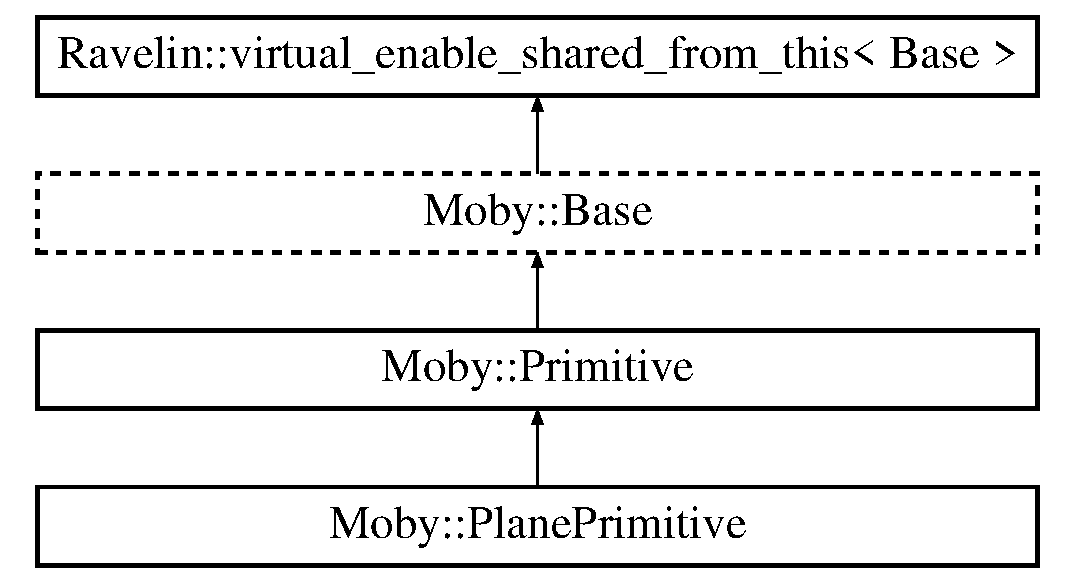
\includegraphics[height=4.000000cm]{classMoby_1_1PlanePrimitive}
\end{center}
\end{figure}
\subsection*{Public Member Functions}
\begin{DoxyCompactItemize}
\item 
{\bf Plane\-Primitive} ()\label{classMoby_1_1PlanePrimitive_a46a405787b15f20af7e822a6bf716aff}

\begin{DoxyCompactList}\small\item\em Initializes the heightmap primitive. \end{DoxyCompactList}\item 
{\bf Plane\-Primitive} (const Ravelin\-::\-Pose3d \&T)\label{classMoby_1_1PlanePrimitive_acec87827c1f4e6628f6f8e3f1b0e75a9}

\begin{DoxyCompactList}\small\item\em Initializes the heightmap primitive. \end{DoxyCompactList}\item 
virtual {\bf Point3d} {\bf get\-\_\-supporting\-\_\-point} (const Ravelin\-::\-Vector3d \&dir) const \label{classMoby_1_1PlanePrimitive_a4c43337b907d7eca31dd7d0ee6732217}

\begin{DoxyCompactList}\small\item\em Gets the supporting point for the plane (for G\-J\-K) \end{DoxyCompactList}\item 
virtual void {\bf set\-\_\-pose} (const Ravelin\-::\-Pose3d \&T)\label{classMoby_1_1PlanePrimitive_a54252ae40e4b18255a441336a98865eb}

\begin{DoxyCompactList}\small\item\em Transforms the primitive. \end{DoxyCompactList}\item 
virtual void {\bf get\-\_\-vertices} (boost\-::shared\-\_\-ptr$<$ const Ravelin\-::\-Pose3d $>$ P, std\-::vector$<$ {\bf Point3d} $>$ \&vertices) const 
\begin{DoxyCompactList}\small\item\em Get vertices corresponding to this primitive. \end{DoxyCompactList}\item 
void {\bfseries get\-\_\-vertices} ({\bf B\-V\-Ptr} bv, boost\-::shared\-\_\-ptr$<$ const Ravelin\-::\-Pose3d $>$ P, std\-::vector$<$ {\bf Point3d} $>$ \&vertices) const \label{classMoby_1_1PlanePrimitive_a44de9591a27ac02b236b41b24e34523d}

\item 
virtual double {\bf calc\-\_\-dist\-\_\-and\-\_\-normal} (const {\bf Point3d} \&point, std\-::vector$<$ Ravelin\-::\-Vector3d $>$ \&normals) const \label{classMoby_1_1PlanePrimitive_a754e5aa58e1feaf4f701ebed8609e67d}

\begin{DoxyCompactList}\small\item\em Finds the signed distance betwen the plane and a point. \end{DoxyCompactList}\item 
virtual double {\bf calc\-\_\-signed\-\_\-dist} (boost\-::shared\-\_\-ptr$<$ const {\bf Primitive} $>$ p, {\bf Point3d} \&pthis, {\bf Point3d} \&pp) const \label{classMoby_1_1PlanePrimitive_a5a04eeb1d16afc20e832414cc67829bb}

\begin{DoxyCompactList}\small\item\em Computes the signed distance between this and another primitive. \end{DoxyCompactList}\item 
double {\bfseries calc\-\_\-signed\-\_\-dist} (boost\-::shared\-\_\-ptr$<$ const {\bf Polyhedral\-Primitive} $>$ b, {\bf Point3d} \&pthis, {\bf Point3d} \&pb) const \label{classMoby_1_1PlanePrimitive_aad41d8cae67e5f20c3aaf86641358134}

\item 
double {\bfseries calc\-\_\-signed\-\_\-dist} (boost\-::shared\-\_\-ptr$<$ const {\bf Cylinder\-Primitive} $>$ s, {\bf Point3d} \&pthis, {\bf Point3d} \&psph) const \label{classMoby_1_1PlanePrimitive_a6c7d5253f56dc7f5dc45b69f04bb8fda}

\item 
double {\bfseries calc\-\_\-signed\-\_\-dist} (boost\-::shared\-\_\-ptr$<$ const {\bf Sphere\-Primitive} $>$ s, {\bf Point3d} \&pthis, {\bf Point3d} \&psph) const \label{classMoby_1_1PlanePrimitive_a9c618fc47c58185ac290354df59b534c}

\item 
virtual double {\bf calc\-\_\-signed\-\_\-dist} (const {\bf Point3d} \&p) const \label{classMoby_1_1PlanePrimitive_a64d68735d467ea55423a1421f108977d}

\begin{DoxyCompactList}\small\item\em Computes the signed distance of the given point from this primitive. \end{DoxyCompactList}\item 
virtual osg\-::\-Node $\ast$ {\bf create\-\_\-visualization} ()\label{classMoby_1_1PlanePrimitive_a2df0aabf6403ae528adbc1b72da179b8}

\begin{DoxyCompactList}\small\item\em Computes the O\-S\-G visualization. \end{DoxyCompactList}\item 
virtual boost\-::shared\-\_\-ptr\\*
$<$ const {\bf Indexed\-Tri\-Array} $>$ {\bf get\-\_\-mesh} (boost\-::shared\-\_\-ptr$<$ const Ravelin\-::\-Pose3d $>$ P)\label{classMoby_1_1PlanePrimitive_a706451877352783453f5141a0a5209ee}

\begin{DoxyCompactList}\small\item\em Gets the mesh of the heightmap. \end{DoxyCompactList}\item 
virtual void {\bfseries calc\-\_\-mass\-\_\-properties} ()\label{classMoby_1_1PlanePrimitive_a05b7ebabe00deb1d511e6f0775e62d88}

\item 
virtual {\bf B\-V\-Ptr} {\bf get\-\_\-\-B\-V\-H\-\_\-root} ({\bf Collision\-Geometry\-Ptr} geom)\label{classMoby_1_1PlanePrimitive_a0366101dd2af4d62e2804f5e4c8722a1}

\begin{DoxyCompactList}\small\item\em Gets the B\-V\-H root for the heightmap. \end{DoxyCompactList}\item 
virtual void {\bf load\-\_\-from\-\_\-xml} (boost\-::shared\-\_\-ptr$<$ const {\bf X\-M\-L\-Tree} $>$ node, std\-::map$<$ std\-::string, {\bf Base\-Ptr} $>$ \&id\-\_\-map)\label{classMoby_1_1PlanePrimitive_ac8093c3e57621aab0884ae91b1e37f5d}

\begin{DoxyCompactList}\small\item\em Implements \doxyref{Base\-::load\-\_\-from\-\_\-xml()}{p.}{classMoby_1_1Base_a98b861c1d615a748b576aa613f17389f} for serialization. \end{DoxyCompactList}\item 
virtual void {\bf save\-\_\-to\-\_\-xml} ({\bf X\-M\-L\-Tree\-Ptr} node, std\-::list$<$ boost\-::shared\-\_\-ptr$<$ const {\bf Base} $>$ $>$ \&shared\-\_\-objects) const \label{classMoby_1_1PlanePrimitive_a860a58e5f0a52e8b6a6c94996e0886d6}

\begin{DoxyCompactList}\small\item\em Implements \doxyref{Base\-::save\-\_\-to\-\_\-xml()}{p.}{classMoby_1_1Base_aed64905ca39893d02d1e6c3f03f73aa9} for serialization. \end{DoxyCompactList}\item 
virtual bool {\bf is\-\_\-convex} () const \label{classMoby_1_1PlanePrimitive_abdd9fe990ba386cf892c90f010506d03}

\begin{DoxyCompactList}\small\item\em Determines whether this primitive is convex. \end{DoxyCompactList}\item 
virtual double {\bfseries get\-\_\-bounding\-\_\-radius} () const \label{classMoby_1_1PlanePrimitive_a90fa0e7cc5427358437b16be1ab60d31}

\end{DoxyCompactItemize}
\subsection*{Protected Member Functions}
\begin{DoxyCompactItemize}
\item 
virtual double {\bf calc\-\_\-height} (const {\bf Point3d} \&p) const \label{classMoby_1_1PlanePrimitive_aa0dde7637cb2abb21195d0dab1fd7657}

\begin{DoxyCompactList}\small\item\em Computes the height at a particular point. \end{DoxyCompactList}\end{DoxyCompactItemize}
\subsection*{Protected Attributes}
\begin{DoxyCompactItemize}
\item 
std\-::map$<$ {\bf Collision\-Geometry\-Ptr}, \\*
boost\-::shared\-\_\-ptr$<$ {\bf O\-B\-B} $>$ $>$ {\bf \-\_\-obbs}\label{classMoby_1_1PlanePrimitive_a76df108c0786d99c484709d174dd1548}

\begin{DoxyCompactList}\small\item\em The bounding volumes for the heightmap. \end{DoxyCompactList}\end{DoxyCompactItemize}
\subsection*{Friends}
\begin{DoxyCompactItemize}
\item 
class {\bfseries C\-C\-D}\label{classMoby_1_1PlanePrimitive_aab79385077be6367d4557d44e17ffcf0}

\end{DoxyCompactItemize}
\subsection*{Additional Inherited Members}


\subsection{Detailed Description}
Represents a heightmap with height zero on the xz plane (primitive can be transformed) 

\subsection{Member Function Documentation}
\index{Moby\-::\-Plane\-Primitive@{Moby\-::\-Plane\-Primitive}!get\-\_\-vertices@{get\-\_\-vertices}}
\index{get\-\_\-vertices@{get\-\_\-vertices}!Moby::PlanePrimitive@{Moby\-::\-Plane\-Primitive}}
\subsubsection[{get\-\_\-vertices}]{\setlength{\rightskip}{0pt plus 5cm}virtual void Moby\-::\-Plane\-Primitive\-::get\-\_\-vertices (
\begin{DoxyParamCaption}
\item[{boost\-::shared\-\_\-ptr$<$ const Ravelin\-::\-Pose3d $>$}]{P, }
\item[{std\-::vector$<$ {\bf Point3d} $>$ \&}]{vertices}
\end{DoxyParamCaption}
) const\hspace{0.3cm}{\ttfamily [virtual]}}\label{classMoby_1_1PlanePrimitive_a86473e30acbf8dd05b8c4305b5f44bc8}


Get vertices corresponding to this primitive. 

Gets the vertex indices from selected facets of an \doxyref{Indexed\-Tri\-Array}{p.}{classMoby_1_1IndexedTriArray}.


\begin{DoxyParams}{Parameters}
{\em tris} & the triangle mesh \\
\hline
{\em fselect\-\_\-begin} & iterator to a container of type unsigned (facet indices) \\
\hline
{\em fselect\-\_\-end} & iterator to a container of type unsigned (facet indices) \\
\hline
{\em output} & beginning iterator to a container of type Point3d; unique vertices are copied here on return \\
\hline
\end{DoxyParams}
\begin{DoxyReturn}{Returns}
ending iterator to a container of type Point3d; unique vertices are copied here on return 
\end{DoxyReturn}


Implements {\bf Moby\-::\-Primitive} \doxyref{}{p.}{classMoby_1_1Primitive_ab50adaba8785794650193def668d4a05}.



The documentation for this class was generated from the following files\-:\begin{DoxyCompactItemize}
\item 
/home/drum/\-Moby/include/\-Moby/Plane\-Primitive.\-h\item 
/home/drum/\-Moby/src/Plane\-Primitive.\-cpp\end{DoxyCompactItemize}

\section{Moby\-:\-:Polyhedral\-Primitive Class Reference}
\label{classMoby_1_1PolyhedralPrimitive}\index{Moby\-::\-Polyhedral\-Primitive@{Moby\-::\-Polyhedral\-Primitive}}


Defines a triangle-\/mesh-\/based primitive type used for inertial property calculation and geometry provisions.  




{\ttfamily \#include $<$Polyhedral\-Primitive.\-h$>$}

Inheritance diagram for Moby\-:\-:Polyhedral\-Primitive\-:\begin{figure}[H]
\begin{center}
\leavevmode
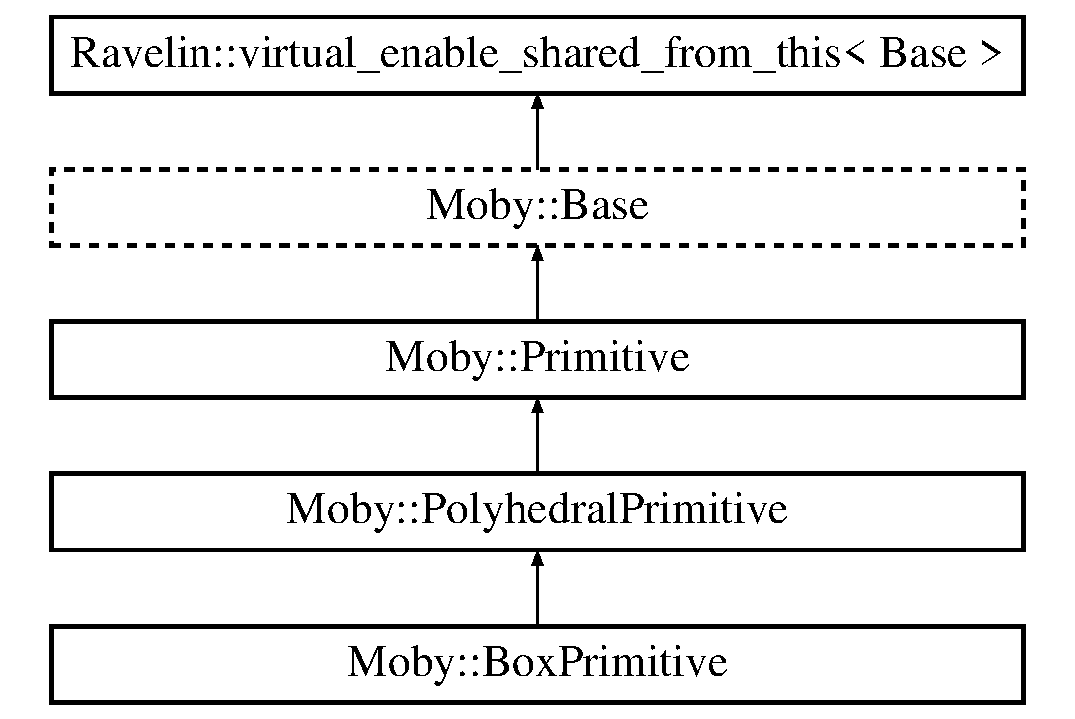
\includegraphics[height=5.000000cm]{classMoby_1_1PolyhedralPrimitive}
\end{center}
\end{figure}
\subsection*{Public Member Functions}
\begin{DoxyCompactItemize}
\item 
{\bfseries Polyhedral\-Primitive} (const Ravelin\-::\-Pose3d \&T)\label{classMoby_1_1PolyhedralPrimitive_a012665335ba4902b7799fd6debf18f4d}

\item 
virtual double {\bf calc\-\_\-signed\-\_\-dist} (boost\-::shared\-\_\-ptr$<$ const {\bf Primitive} $>$ p, {\bf Point3d} \&pthis, {\bf Point3d} \&pp) const \label{classMoby_1_1PolyhedralPrimitive_a61245f02fe06f76859b66392adfd2299}

\begin{DoxyCompactList}\small\item\em Computes the signed distance between this and another primitive. \end{DoxyCompactList}\item 
virtual double {\bf calc\-\_\-dist\-\_\-and\-\_\-normal} (const {\bf Point3d} \&p, std\-::vector$<$ Ravelin\-::\-Vector3d $>$ \&normals) const \label{classMoby_1_1PolyhedralPrimitive_a22722fd738a89219d3b908cb1a4ad01b}

\begin{DoxyCompactList}\small\item\em Computes the distance between a point and this primitive. \end{DoxyCompactList}\item 
virtual osg\-::\-Node $\ast$ {\bf create\-\_\-visualization} ()\label{classMoby_1_1PolyhedralPrimitive_afa28b33a3714c5a0b1289fff75f6caf4}

\begin{DoxyCompactList}\small\item\em creates the visualization for the primitive \end{DoxyCompactList}\item 
virtual {\bf B\-V\-Ptr} {\bf get\-\_\-\-B\-V\-H\-\_\-root} ({\bf Collision\-Geometry\-Ptr} geom)\label{classMoby_1_1PolyhedralPrimitive_ae10c91e74bfff9bbef18669cffd801cc}

\begin{DoxyCompactList}\small\item\em Gets the root bounding volume for this primitive. \end{DoxyCompactList}\item 
virtual void {\bf set\-\_\-polyhedron} (const {\bf Polyhedron} \&p)
\begin{DoxyCompactList}\small\item\em Sets the polyhedron corresponding to this primitive. \end{DoxyCompactList}\item 
virtual void {\bf get\-\_\-vertices} (boost\-::shared\-\_\-ptr$<$ const Ravelin\-::\-Pose3d $>$ P, std\-::vector$<$ {\bf Point3d} $>$ \&vertices) const 
\begin{DoxyCompactList}\small\item\em Get vertices corresponding to this primitive. \end{DoxyCompactList}\item 
virtual boost\-::shared\-\_\-ptr\\*
$<$ const {\bf Indexed\-Tri\-Array} $>$ {\bf get\-\_\-mesh} (boost\-::shared\-\_\-ptr$<$ const Ravelin\-::\-Pose3d $>$ P)\label{classMoby_1_1PolyhedralPrimitive_a33762e3c23305eb7802287e2c8526b6c}

\begin{DoxyCompactList}\small\item\em Gets the underlying triangle mesh for this primitive. \end{DoxyCompactList}\item 
virtual bool {\bf is\-\_\-convex} () const \label{classMoby_1_1PolyhedralPrimitive_a82c2d78f556315969eac46c42e6698ef}

\begin{DoxyCompactList}\small\item\em Determines whether the primitive is convex. \end{DoxyCompactList}\item 
virtual void {\bf load\-\_\-from\-\_\-xml} (boost\-::shared\-\_\-ptr$<$ const {\bf X\-M\-L\-Tree} $>$ node, std\-::map$<$ std\-::string, {\bf Base\-Ptr} $>$ \&id\-\_\-map)\label{classMoby_1_1PolyhedralPrimitive_a54ede66e39b6ae57827a6cbeb9480335}

\begin{DoxyCompactList}\small\item\em Implements \doxyref{Base\-::load\-\_\-from\-\_\-xml()}{p.}{classMoby_1_1Base_a98b861c1d615a748b576aa613f17389f} for serialization. \end{DoxyCompactList}\item 
virtual void {\bf save\-\_\-to\-\_\-xml} ({\bf X\-M\-L\-Tree\-Ptr} node, std\-::list$<$ boost\-::shared\-\_\-ptr$<$ const {\bf Base} $>$ $>$ \&shared\-\_\-objects) const \label{classMoby_1_1PolyhedralPrimitive_a2c023ea6208e9817586997ac753d506e}

\begin{DoxyCompactList}\small\item\em Implements \doxyref{Base\-::save\-\_\-to\-\_\-xml()}{p.}{classMoby_1_1Base_aed64905ca39893d02d1e6c3f03f73aa9} for serialization. \end{DoxyCompactList}\item 
virtual void {\bf set\-\_\-pose} (const Ravelin\-::\-Pose3d \&P)\label{classMoby_1_1PolyhedralPrimitive_a30ccf2649b4f3b48c92db6b444e5790f}

\begin{DoxyCompactList}\small\item\em Sets the pose of this primitive. \end{DoxyCompactList}\item 
const {\bf Polyhedron} \& {\bf get\-\_\-polyhedron} () const \label{classMoby_1_1PolyhedralPrimitive_a1f8940bc0f00cd65855538cbe58ab6c2}

\begin{DoxyCompactList}\small\item\em Gets the polyhedron corresponding to this primitive (in its transformed state) \end{DoxyCompactList}\item 
virtual unsigned {\bfseries num\-\_\-facets} () const \label{classMoby_1_1PolyhedralPrimitive_a2b61a8d162299d0ecbaca9960f72a022}

\item 
virtual double {\bfseries get\-\_\-bounding\-\_\-radius} () const \label{classMoby_1_1PolyhedralPrimitive_ad5fd6180e5a653b11fcdd0939c6dc6b4}

\item 
{\footnotesize template$<$class Output\-Iterator $>$ }\\Output\-Iterator {\bfseries get\-\_\-halfspaces} (const {\bf Polyhedron} \&poly, boost\-::shared\-\_\-ptr$<$ const Ravelin\-::\-Pose3d $>$ pose, const Ravelin\-::\-Transform3d \&w\-Tpose, Output\-Iterator output\-\_\-begin)\label{classMoby_1_1PolyhedralPrimitive_a7352a6f8dbbf7ccdd143d6dea7bb30cd}

\end{DoxyCompactItemize}
\subsection*{Static Public Member Functions}
\begin{DoxyCompactItemize}
\item 
{\footnotesize template$<$class Output\-Iterator $>$ }\\static Output\-Iterator {\bfseries get\-\_\-halfspaces} (const {\bf Polyhedron} \&poly, boost\-::shared\-\_\-ptr$<$ const Ravelin\-::\-Pose3d $>$ pose, const Ravelin\-::\-Transform3d \&w\-Tpose, Output\-Iterator output\-\_\-begin)\label{classMoby_1_1PolyhedralPrimitive_a7352a6f8dbbf7ccdd143d6dea7bb30cd}

\end{DoxyCompactItemize}
\subsection*{Protected Member Functions}
\begin{DoxyCompactItemize}
\item 
void {\bf calc\-\_\-mass\-\_\-properties} ()\label{classMoby_1_1PolyhedralPrimitive_a0fba37da49ac3145ec9e32b0d274c579}

\begin{DoxyCompactList}\small\item\em Calculates mass properties for the polyhedron. \end{DoxyCompactList}\item 
double {\bfseries calc\-\_\-signed\-\_\-dist} (boost\-::shared\-\_\-ptr$<$ const {\bf Polyhedral\-Primitive} $>$ p, {\bf Point3d} \&pthis, {\bf Point3d} \&pp) const \label{classMoby_1_1PolyhedralPrimitive_aaf38b41346a68e7b80918c556b01fd32}

\end{DoxyCompactItemize}
\subsection*{Protected Attributes}
\begin{DoxyCompactItemize}
\item 
{\bf Polyhedron} {\bfseries \-\_\-poly}\label{classMoby_1_1PolyhedralPrimitive_abe686fe1473a0d38257ad086f2f6fc58}

\end{DoxyCompactItemize}
\subsection*{Additional Inherited Members}


\subsection{Detailed Description}
Defines a triangle-\/mesh-\/based primitive type used for inertial property calculation and geometry provisions. 

The center-\/of-\/mass of derived types may be at the origin of the world, or not. Additionally, \doxyref{Primitive}{p.}{classMoby_1_1Primitive} can take a transformation matrix in its constructor, with which the primitive data (com, inertia matrix, and geometry) can be transformed. 

\subsection{Member Function Documentation}
\index{Moby\-::\-Polyhedral\-Primitive@{Moby\-::\-Polyhedral\-Primitive}!get\-\_\-vertices@{get\-\_\-vertices}}
\index{get\-\_\-vertices@{get\-\_\-vertices}!Moby::PolyhedralPrimitive@{Moby\-::\-Polyhedral\-Primitive}}
\subsubsection[{get\-\_\-vertices}]{\setlength{\rightskip}{0pt plus 5cm}void Polyhedral\-Primitive\-::get\-\_\-vertices (
\begin{DoxyParamCaption}
\item[{boost\-::shared\-\_\-ptr$<$ const Ravelin\-::\-Pose3d $>$}]{P, }
\item[{std\-::vector$<$ {\bf Point3d} $>$ \&}]{vertices}
\end{DoxyParamCaption}
) const\hspace{0.3cm}{\ttfamily [virtual]}}\label{classMoby_1_1PolyhedralPrimitive_a7466ac4071e3710894bf8c002026cd3f}


Get vertices corresponding to this primitive. 

Gets the vertex indices from selected facets of an \doxyref{Indexed\-Tri\-Array}{p.}{classMoby_1_1IndexedTriArray}.


\begin{DoxyParams}{Parameters}
{\em tris} & the triangle mesh \\
\hline
{\em fselect\-\_\-begin} & iterator to a container of type unsigned (facet indices) \\
\hline
{\em fselect\-\_\-end} & iterator to a container of type unsigned (facet indices) \\
\hline
{\em output} & beginning iterator to a container of type Point3d; unique vertices are copied here on return \\
\hline
\end{DoxyParams}
\begin{DoxyReturn}{Returns}
ending iterator to a container of type Point3d; unique vertices are copied here on return 
\end{DoxyReturn}


Implements {\bf Moby\-::\-Primitive} \doxyref{}{p.}{classMoby_1_1Primitive_ab50adaba8785794650193def668d4a05}.



Reimplemented in {\bf Moby\-::\-Box\-Primitive} \doxyref{}{p.}{classMoby_1_1BoxPrimitive_a329b84ac213b791173b787fb54996e6c}.

\index{Moby\-::\-Polyhedral\-Primitive@{Moby\-::\-Polyhedral\-Primitive}!set\-\_\-polyhedron@{set\-\_\-polyhedron}}
\index{set\-\_\-polyhedron@{set\-\_\-polyhedron}!Moby::PolyhedralPrimitive@{Moby\-::\-Polyhedral\-Primitive}}
\subsubsection[{set\-\_\-polyhedron}]{\setlength{\rightskip}{0pt plus 5cm}void Polyhedral\-Primitive\-::set\-\_\-polyhedron (
\begin{DoxyParamCaption}
\item[{const {\bf Polyhedron} \&}]{p}
\end{DoxyParamCaption}
)\hspace{0.3cm}{\ttfamily [virtual]}}\label{classMoby_1_1PolyhedralPrimitive_ae5f4a9141ad1b6d74b6997fe5d829c6f}


Sets the polyhedron corresponding to this primitive. 

Should only be done when the primitive hasn't been transformed. 

Reimplemented in {\bf Moby\-::\-Box\-Primitive} \doxyref{}{p.}{classMoby_1_1BoxPrimitive_a6a4bb0ee868ece8fdf982e7058de6714}.



The documentation for this class was generated from the following files\-:\begin{DoxyCompactItemize}
\item 
/home/drum/\-Moby/include/\-Moby/Polyhedral\-Primitive.\-h\item 
/home/drum/\-Moby/include/\-Moby/Polyhedral\-Primitive.\-inl\item 
/home/drum/\-Moby/src/Polyhedral\-Primitive.\-cpp\end{DoxyCompactItemize}

\section{Moby\-:\-:Polyhedron Class Reference}
\label{classMoby_1_1Polyhedron}\index{Moby\-::\-Polyhedron@{Moby\-::\-Polyhedron}}


A potentially-\/non-\/convex polyhedron of genus 0.  




{\ttfamily \#include $<$Polyhedron.\-h$>$}

\subsection*{Classes}
\begin{DoxyCompactItemize}
\item 
struct {\bf Edge}
\begin{DoxyCompactList}\small\item\em The edge structure. \end{DoxyCompactList}\item 
struct {\bf Face}
\begin{DoxyCompactList}\small\item\em The face structure. \end{DoxyCompactList}\item 
struct {\bf Feature}
\begin{DoxyCompactList}\small\item\em A vertex, face, or edge in a polyhedron. \end{DoxyCompactList}\item 
struct {\bf Vertex}
\begin{DoxyCompactList}\small\item\em The vertex structure. \end{DoxyCompactList}\item 
class {\bf Vertex\-Face\-Iterator}
\begin{DoxyCompactList}\small\item\em iterates over the vertices in a face \end{DoxyCompactList}\end{DoxyCompactItemize}
\subsection*{Public Types}
\begin{DoxyCompactItemize}
\item 
enum {\bfseries Location\-Type} \{ \\*
{\bfseries e\-Inside}, 
{\bfseries e\-Outside}, 
{\bfseries e\-On\-Vertex}, 
{\bfseries e\-On\-Edge}, 
\\*
{\bfseries e\-On\-Face}
 \}
\item 
enum {\bf Feature\-Type} \{ {\bfseries e\-Vertex}, 
{\bfseries e\-Edge}, 
{\bfseries e\-Face}
 \}
\begin{DoxyCompactList}\small\item\em Gets the Voronoi plane from two input features. \end{DoxyCompactList}\end{DoxyCompactItemize}
\subsection*{Public Member Functions}
\begin{DoxyCompactItemize}
\item 
{\bf Polyhedron} ()\label{classMoby_1_1Polyhedron_aebdf7ee85eb636069bf93afb4e6a483f}

\begin{DoxyCompactList}\small\item\em Creates a minimum polyhedron. \end{DoxyCompactList}\item 
{\bfseries Polyhedron} (const {\bf Polyhedron} \&p)\label{classMoby_1_1Polyhedron_a78d58f579539183b64839e85a7886c7f}

\item 
boost\-::shared\-\_\-ptr\\*
$<$ {\bf Polyhedron\-::\-Feature} $>$ {\bf find\-\_\-closest\-\_\-feature} (const Ravelin\-::\-Origin3d \&p, unsigned closest\-\_\-facet) const 
\begin{DoxyCompactList}\small\item\em Finds the closest feature of the polyhedron to the point, given the closest facet. \end{DoxyCompactList}\item 
{\bf Polyhedron} \& {\bf operator=} (const {\bf Polyhedron} \&p)\label{classMoby_1_1Polyhedron_a4cee7a5bf6546f2d6c4a0904f005a40a}

\begin{DoxyCompactList}\small\item\em Assignment operator. \end{DoxyCompactList}\item 
{\bf Polyhedron} {\bf shallow\-\_\-copy} () const \label{classMoby_1_1Polyhedron_a649f6aa1c7f3707e955be1544751c4ea}

\begin{DoxyCompactList}\small\item\em Does a shallow copy of this polyhedron. \end{DoxyCompactList}\item 
std\-::vector$<$ boost\-::shared\-\_\-ptr\\*
$<$ {\bf Vertex} $>$ $>$ \& {\bfseries get\-\_\-vertices} ()\label{classMoby_1_1Polyhedron_ade11893c4a4825958f0a21fc3cfa587f}

\item 
const std\-::vector\\*
$<$ boost\-::shared\-\_\-ptr$<$ {\bf Vertex} $>$ $>$ \& {\bfseries get\-\_\-vertices} () const \label{classMoby_1_1Polyhedron_a43576df898c75c40c036fdffba2d97fe}

\item 
const std\-::vector\\*
$<$ boost\-::shared\-\_\-ptr$<$ {\bf Edge} $>$ $>$ \& {\bfseries get\-\_\-edges} () const \label{classMoby_1_1Polyhedron_ad3c45794cf83d79fb425d667e571f4a9}

\item 
const std\-::vector\\*
$<$ boost\-::shared\-\_\-ptr$<$ {\bf Face} $>$ $>$ \& {\bfseries get\-\_\-faces} () const \label{classMoby_1_1Polyhedron_a2a2974b6fa0f1c42fdaa3267f6ab2c1b}

\item 
bool {\bfseries inside} (const Ravelin\-::\-Origin3d \&point, double tol=N\-E\-A\-R\-\_\-\-Z\-E\-R\-O)\label{classMoby_1_1Polyhedron_a9da6cd5a5dbf85e81a1c3c218d7d9112}

\item 
bool {\bfseries inside\-\_\-or\-\_\-on} (const Ravelin\-::\-Origin3d \&point, double tol=N\-E\-A\-R\-\_\-\-Z\-E\-R\-O)\label{classMoby_1_1Polyhedron_a1c0701c018cb23aca27a6eef2752f3cc}

\item 
Location\-Type {\bfseries location} (const Ravelin\-::\-Origin3d \&point, boost\-::shared\-\_\-ptr$<$ {\bf Polyhedron\-::\-Feature} $>$ \&closest\-\_\-feature, double tol=N\-E\-A\-R\-\_\-\-Z\-E\-R\-O) const \label{classMoby_1_1Polyhedron_a1079176623c9cce5d821f528c6397c28}

\item 
double {\bfseries calc\-\_\-volume} () const \label{classMoby_1_1Polyhedron_a9b96a5f4b186cbaed6d38d8470ee52db}

\item 
bool {\bfseries degenerate} () const \label{classMoby_1_1Polyhedron_a8341c94887c6f4489ecbb0954394e2a5}

\item 
void {\bf write\-\_\-to\-\_\-obj} (const std\-::string \&filename) const \label{classMoby_1_1Polyhedron_aad211929a05398f8df28f932c7a73888}

\begin{DoxyCompactList}\small\item\em Writes the polyhedron to Wavefront O\-B\-J format. \end{DoxyCompactList}\item 
{\bf Polyhedron} {\bf transform} (const Ravelin\-::\-Transform3d \&T) const \label{classMoby_1_1Polyhedron_a2d054dfef9a6039cc661e5ebe9a1f100}

\begin{DoxyCompactList}\small\item\em Transforms a polyhedron. \end{DoxyCompactList}\item 
double {\bf calc\-\_\-signed\-\_\-distance} (const Ravelin\-::\-Origin3d \&point, unsigned \&closest\-\_\-facet) const \label{classMoby_1_1Polyhedron_a75fe654af8a515961ee498115b7f9bfc}

\begin{DoxyCompactList}\small\item\em Gets the signed distance and closest facet to a point. \end{DoxyCompactList}\item 
double {\bf calc\-\_\-signed\-\_\-distance} (const Ravelin\-::\-Origin3d \&point) const \label{classMoby_1_1Polyhedron_a5ecb8756efc37a78f3c2a7a6833ae367}

\begin{DoxyCompactList}\small\item\em Gets the signed distance from a point to the polyhedron. \end{DoxyCompactList}\item 
std\-::pair$<$ Ravelin\-::\-Origin3d, \\*
Ravelin\-::\-Origin3d $>$ {\bf get\-\_\-bounding\-\_\-box\-\_\-corners} () const \label{classMoby_1_1Polyhedron_aa812e2865477420a867ec58e0192eba8}

\begin{DoxyCompactList}\small\item\em Gets the corners of the axis-\/aligned bounding box of this polyhedron. \end{DoxyCompactList}\item 
bool {\bf is\-\_\-convex} ()\label{classMoby_1_1Polyhedron_a0517cc02de0d0df45b1c30333303ed29}

\begin{DoxyCompactList}\small\item\em Determines whether this polyhedron convex (to w/in floating point tolerance) \end{DoxyCompactList}\item 
double {\bf convexity} ()
\begin{DoxyCompactList}\small\item\em Gets the convexity of this polyhedron. \end{DoxyCompactList}\item 
{\footnotesize template$<$class Forward\-Iterator $>$ }\\{\bf Polyhedron} {\bf calc\-\_\-convex\-\_\-hull} (Forward\-Iterator begin, Forward\-Iterator end)\label{classMoby_1_1Polyhedron_ab5c6b4a9e78a7f780cd94148340c705b}

\begin{DoxyCompactList}\small\item\em Computes the convex hull for a polyhedron. \end{DoxyCompactList}\end{DoxyCompactItemize}
\subsection*{Static Public Member Functions}
\begin{DoxyCompactItemize}
\item 
static double {\bf vclip} (boost\-::shared\-\_\-ptr$<$ const {\bf Polyhedral\-Primitive} $>$ p\-A, boost\-::shared\-\_\-ptr$<$ const {\bf Polyhedral\-Primitive} $>$ p\-B, boost\-::shared\-\_\-ptr$<$ const Ravelin\-::\-Pose3d $>$ pose\-A, boost\-::shared\-\_\-ptr$<$ const Ravelin\-::\-Pose3d $>$ pose\-B, boost\-::shared\-\_\-ptr$<$ const {\bf Polyhedron\-::\-Feature} $>$ \&closest\-A, boost\-::shared\-\_\-ptr$<$ const {\bf Polyhedron\-::\-Feature} $>$ \&closest\-B)\label{classMoby_1_1Polyhedron_a5d653baf20939d27fe37787c79432b31}

\begin{DoxyCompactList}\small\item\em Executes the V-\/\-Clip algorithm on two polyhedra, determining closest features and signed distance. \end{DoxyCompactList}\item 
static {\bf Polyhedron} {\bf calc\-\_\-minkowski\-\_\-diff} (boost\-::shared\-\_\-ptr$<$ const {\bf Polyhedral\-Primitive} $>$ p\-A, boost\-::shared\-\_\-ptr$<$ const {\bf Polyhedral\-Primitive} $>$ p\-B, boost\-::shared\-\_\-ptr$<$ const Ravelin\-::\-Pose3d $>$ pose\-A, boost\-::shared\-\_\-ptr$<$ const Ravelin\-::\-Pose3d $>$ pose\-B)
\begin{DoxyCompactList}\small\item\em Computes the Minkowski difference of two polyhedral primitives. \end{DoxyCompactList}\item 
static void {\bf to\-\_\-vrml} (std\-::ostream \&out, const {\bf Polyhedron} \&p, Ravelin\-::\-Origin3d diffuse\-\_\-color=Ravelin\-::\-Origin3d(1, 1, 1), bool wireframe=false)
\begin{DoxyCompactList}\small\item\em Finds the feature(s) of this polyhedron closest to the point. \end{DoxyCompactList}\item 
{\footnotesize template$<$class Forward\-Iterator $>$ }\\static {\bf Polyhedron} {\bf calc\-\_\-convex\-\_\-hull} (Forward\-Iterator begin, Forward\-Iterator end)\label{classMoby_1_1Polyhedron_ab5c6b4a9e78a7f780cd94148340c705b}

\begin{DoxyCompactList}\small\item\em Computes the convex hull for a polyhedron. \end{DoxyCompactList}\item 
static double {\bf calc\-\_\-dist} ({\bf Feature\-Type} f\-A, {\bf Feature\-Type} f\-B, boost\-::shared\-\_\-ptr$<$ const {\bf Polyhedron\-::\-Feature} $>$ closest\-A, boost\-::shared\-\_\-ptr$<$ const {\bf Polyhedron\-::\-Feature} $>$ closest\-B, Ravelin\-::\-Transform3d \&a\-Tb)\label{classMoby_1_1Polyhedron_a7f6f47191dcb708b10f04c9cf1786ff7}

\begin{DoxyCompactList}\small\item\em Computes the distance between two features. \end{DoxyCompactList}\end{DoxyCompactItemize}
\subsection*{Friends}
\begin{DoxyCompactItemize}
\item 
class {\bfseries Tessellated\-Polyhedron}\label{classMoby_1_1Polyhedron_aa256fdce053f102562b540cceee239f1}

\end{DoxyCompactItemize}


\subsection{Detailed Description}
A potentially-\/non-\/convex polyhedron of genus 0. 

\subsection{Member Enumeration Documentation}
\index{Moby\-::\-Polyhedron@{Moby\-::\-Polyhedron}!Feature\-Type@{Feature\-Type}}
\index{Feature\-Type@{Feature\-Type}!Moby::Polyhedron@{Moby\-::\-Polyhedron}}
\subsubsection[{Feature\-Type}]{\setlength{\rightskip}{0pt plus 5cm}enum {\bf Moby\-::\-Polyhedron\-::\-Feature\-Type}}\label{classMoby_1_1Polyhedron_a9eeae159b2e4a6fbbfb0948dd0bbbfeb}


Gets the Voronoi plane from two input features. 

The function takes the tyoes and the pointers of the two features and returns a plane If a point is a positive distance away from the plane, then the point is closer to the first feature If a point is a negative distance away from the plane, then the point is closer to the second feature 

\subsection{Member Function Documentation}
\index{Moby\-::\-Polyhedron@{Moby\-::\-Polyhedron}!calc\-\_\-minkowski\-\_\-diff@{calc\-\_\-minkowski\-\_\-diff}}
\index{calc\-\_\-minkowski\-\_\-diff@{calc\-\_\-minkowski\-\_\-diff}!Moby::Polyhedron@{Moby\-::\-Polyhedron}}
\subsubsection[{calc\-\_\-minkowski\-\_\-diff}]{\setlength{\rightskip}{0pt plus 5cm}{\bf Polyhedron} Polyhedron\-::calc\-\_\-minkowski\-\_\-diff (
\begin{DoxyParamCaption}
\item[{boost\-::shared\-\_\-ptr$<$ const {\bf Polyhedral\-Primitive} $>$}]{p\-A, }
\item[{boost\-::shared\-\_\-ptr$<$ const {\bf Polyhedral\-Primitive} $>$}]{p\-B, }
\item[{boost\-::shared\-\_\-ptr$<$ const Ravelin\-::\-Pose3d $>$}]{pose\-A, }
\item[{boost\-::shared\-\_\-ptr$<$ const Ravelin\-::\-Pose3d $>$}]{pose\-B}
\end{DoxyParamCaption}
)\hspace{0.3cm}{\ttfamily [static]}}\label{classMoby_1_1Polyhedron_abf2470d62080fd4749866623fdb5a012}


Computes the Minkowski difference of two polyhedral primitives. 

\begin{DoxyReturn}{Returns}
a polyhedron-\/ the 'data' field of each vertex is of type boost\-::shared\-\_\-ptr$<$std\-::pair$<$int, int$>$ $>$, where the first integer is the index of a vertex from the first polyhedron and the second integer is the index of a vertex from the second polyhedron. 
\end{DoxyReturn}
\index{Moby\-::\-Polyhedron@{Moby\-::\-Polyhedron}!convexity@{convexity}}
\index{convexity@{convexity}!Moby::Polyhedron@{Moby\-::\-Polyhedron}}
\subsubsection[{convexity}]{\setlength{\rightskip}{0pt plus 5cm}double Moby\-::\-Polyhedron\-::convexity (
\begin{DoxyParamCaption}
{}
\end{DoxyParamCaption}
)\hspace{0.3cm}{\ttfamily [inline]}}\label{classMoby_1_1Polyhedron_a3b4fe0b22821116e8360c5e70f1ead58}


Gets the convexity of this polyhedron. 

Convexity values less than epsilon (where epsilon is some number near zero) indicate that the polyhedron is convex; greater values indicate that the polyhedron is non-\/convex. 

Referenced by is\-\_\-convex().

\index{Moby\-::\-Polyhedron@{Moby\-::\-Polyhedron}!find\-\_\-closest\-\_\-feature@{find\-\_\-closest\-\_\-feature}}
\index{find\-\_\-closest\-\_\-feature@{find\-\_\-closest\-\_\-feature}!Moby::Polyhedron@{Moby\-::\-Polyhedron}}
\subsubsection[{find\-\_\-closest\-\_\-feature}]{\setlength{\rightskip}{0pt plus 5cm}boost\-::shared\-\_\-ptr$<$ {\bf Polyhedron\-::\-Feature} $>$ Polyhedron\-::find\-\_\-closest\-\_\-feature (
\begin{DoxyParamCaption}
\item[{const Ravelin\-::\-Origin3d \&}]{p, }
\item[{unsigned}]{closest\-\_\-facet}
\end{DoxyParamCaption}
) const}\label{classMoby_1_1Polyhedron_aba14204a10759717c3ac6c29ea192bf6}


Finds the closest feature of the polyhedron to the point, given the closest facet. 


\begin{DoxyParams}{Parameters}
{\em closest\-\_\-facet} & the closest facet to the point on return \\
\hline
\end{DoxyParams}
\index{Moby\-::\-Polyhedron@{Moby\-::\-Polyhedron}!to\-\_\-vrml@{to\-\_\-vrml}}
\index{to\-\_\-vrml@{to\-\_\-vrml}!Moby::Polyhedron@{Moby\-::\-Polyhedron}}
\subsubsection[{to\-\_\-vrml}]{\setlength{\rightskip}{0pt plus 5cm}void Polyhedron\-::to\-\_\-vrml (
\begin{DoxyParamCaption}
\item[{std\-::ostream \&}]{out, }
\item[{const {\bf Polyhedron} \&}]{p, }
\item[{Ravelin\-::\-Origin3d}]{diffuse\-\_\-color = {\ttfamily Ravelin\-:\-:Origin3d(1,1,1)}, }
\item[{bool}]{wireframe = {\ttfamily false}}
\end{DoxyParamCaption}
)\hspace{0.3cm}{\ttfamily [static]}}\label{classMoby_1_1Polyhedron_a25e33c1c9b67e8bb297c8fb70f037a72}


Finds the feature(s) of this polyhedron closest to the point. 


\begin{DoxyParams}{Parameters}
{\em p} & the query point \\
\hline
{\em closest\-\_\-features} & the closest features on return \\
\hline
{\em inside} & whether the point is inside or outside the polyhedron on return \\
\hline
\end{DoxyParams}
\begin{DoxyReturn}{Returns}
the distance\-Sends this polyhedron to the specified stream using V\-R\-M\-L 
\end{DoxyReturn}


References Moby\-::\-Polyhedron\-::\-Vertex\-Face\-Iterator\-::advance(), and Moby\-::\-Polyhedron\-::\-Vertex\-Face\-Iterator\-::has\-\_\-next().



The documentation for this class was generated from the following files\-:\begin{DoxyCompactItemize}
\item 
/home/drum/\-Moby/include/\-Moby/Polyhedron.\-h\item 
/home/drum/\-Moby/include/\-Moby/Polyhedron.\-inl\item 
/home/drum/\-Moby/src/Polyhedron.\-cpp\end{DoxyCompactItemize}

\section{Moby\-:\-:Primitive Class Reference}
\label{classMoby_1_1Primitive}\index{Moby\-::\-Primitive@{Moby\-::\-Primitive}}


Defines a triangle-\/mesh-\/based primitive type used for inertial property calculation and geometry provisions.  




{\ttfamily \#include $<$Primitive.\-h$>$}

Inheritance diagram for Moby\-:\-:Primitive\-:\begin{figure}[H]
\begin{center}
\leavevmode
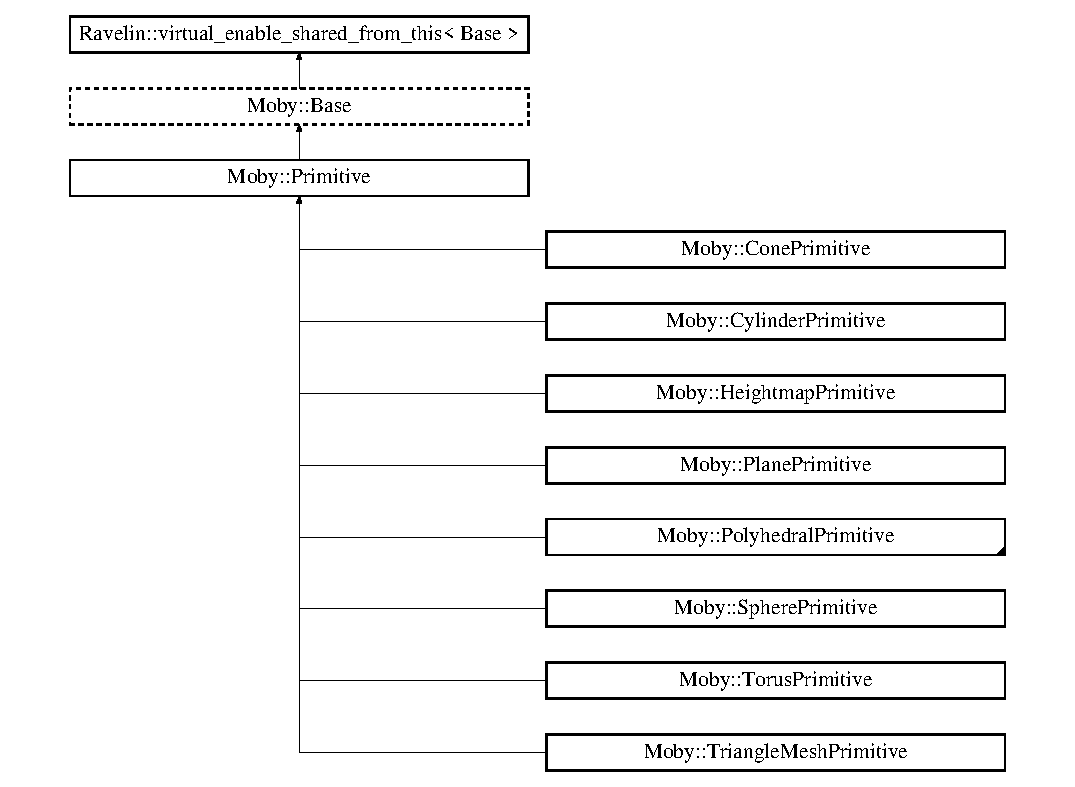
\includegraphics[height=10.131579cm]{classMoby_1_1Primitive}
\end{center}
\end{figure}
\subsection*{Public Member Functions}
\begin{DoxyCompactItemize}
\item 
{\bf Primitive} ()\label{classMoby_1_1Primitive_ae6b6e9440d482575d1dcbf77a936c201}

\begin{DoxyCompactList}\small\item\em Constructs a primitive under the identity transformation. \end{DoxyCompactList}\item 
{\bfseries Primitive} (const Ravelin\-::\-Pose3d \&T)\label{classMoby_1_1Primitive_ac005739f92deab6182ad9b887413e5cf}

\item 
virtual void {\bf load\-\_\-from\-\_\-xml} (boost\-::shared\-\_\-ptr$<$ const {\bf X\-M\-L\-Tree} $>$ node, std\-::map$<$ std\-::string, {\bf Base\-Ptr} $>$ \&id\-\_\-map)\label{classMoby_1_1Primitive_ab2cb5a7043032a8a3df736909740d1f7}

\begin{DoxyCompactList}\small\item\em Implements \doxyref{Base\-::load\-\_\-from\-\_\-xml()}{p.}{classMoby_1_1Base_a98b861c1d615a748b576aa613f17389f} for serialization. \end{DoxyCompactList}\item 
virtual void {\bf save\-\_\-to\-\_\-xml} ({\bf X\-M\-L\-Tree\-Ptr} node, std\-::list$<$ boost\-::shared\-\_\-ptr$<$ const {\bf Base} $>$ $>$ \&shared\-\_\-objects) const \label{classMoby_1_1Primitive_aa5925c970e939796f5fd07d1c8198437}

\begin{DoxyCompactList}\small\item\em Implements \doxyref{Base\-::save\-\_\-to\-\_\-xml()}{p.}{classMoby_1_1Base_aed64905ca39893d02d1e6c3f03f73aa9} for serialization. \end{DoxyCompactList}\item 
void {\bf update\-\_\-visualization} ()\label{classMoby_1_1Primitive_a89ee97934a86698bbfedeb603e7b17ad}

\begin{DoxyCompactList}\small\item\em Updates the visualization on the primitive. \end{DoxyCompactList}\item 
void {\bf set\-\_\-mass} (double mass)
\begin{DoxyCompactList}\small\item\em Sets the mass of this primitive. \end{DoxyCompactList}\item 
void {\bf set\-\_\-density} (double density)\label{classMoby_1_1Primitive_a4237eca57396dbb01e07a8ebb376b5e9}

\begin{DoxyCompactList}\small\item\em Sets the density of this primitive. \end{DoxyCompactList}\item 
virtual void {\bf set\-\_\-pose} (const Ravelin\-::\-Pose3d \&T)\label{classMoby_1_1Primitive_a136eb09810531c47a0da93ef70534950}

\begin{DoxyCompactList}\small\item\em Sets the transform for this primitive -- transforms mesh and inertial properties (if calculated) \end{DoxyCompactList}\item 
virtual {\bf Point3d} {\bf get\-\_\-supporting\-\_\-point} (const Ravelin\-::\-Vector3d \&d) const \label{classMoby_1_1Primitive_a497607bdbb73e48cd4eaa4cfb3a34502}

\begin{DoxyCompactList}\small\item\em Gets a supporting point from a primitive. \end{DoxyCompactList}\item 
virtual double {\bf calc\-\_\-signed\-\_\-dist} (const {\bf Point3d} \&p) const \label{classMoby_1_1Primitive_a06829f79f039faea7f23460036c913b5}

\begin{DoxyCompactList}\small\item\em Calculates the signed distance from this primitive. \end{DoxyCompactList}\item 
void {\bf add\-\_\-collision\-\_\-geometry} ({\bf Collision\-Geometry\-Ptr} cg)\label{classMoby_1_1Primitive_aa6db4769773cc5fd99032df52f73d681}

\begin{DoxyCompactList}\small\item\em Adds a collision geometry. \end{DoxyCompactList}\item 
void {\bf remove\-\_\-collision\-\_\-geometry} ({\bf Collision\-Geometry\-Ptr} cg)\label{classMoby_1_1Primitive_afb386d7c5d657b773084647e6ce81b6d}

\begin{DoxyCompactList}\small\item\em Removes a collision geometry. \end{DoxyCompactList}\item 
boost\-::shared\-\_\-ptr$<$ const \\*
Ravelin\-::\-Pose3d $>$ {\bf get\-\_\-pose} ({\bf Collision\-Geometry\-Ptr} g) const \label{classMoby_1_1Primitive_a15029c143c9a8b28c454bbfc7146aa2b}

\begin{DoxyCompactList}\small\item\em Gets the pose of this primitive relative to a particular collision geometry. \end{DoxyCompactList}\item 
virtual double {\bfseries get\-\_\-bounding\-\_\-radius} () const =0\label{classMoby_1_1Primitive_a291847b5c5eb652edb56116240a29fe7}

\item 
virtual double {\bf calc\-\_\-max\-\_\-dist} (double lin\-\_\-cont, double ang\-\_\-cont, double dist, const Ravelin\-::\-Vector3d \&d0, const Ravelin\-::\-Vector3d \&w0, boost\-::shared\-\_\-ptr$<$ const Ravelin\-::\-Pose3d $>$ P)\label{classMoby_1_1Primitive_ae9ec4a781a67b5b223acf0c25eb3637d}

\begin{DoxyCompactList}\small\item\em Computes the maximum distance by a point on the geometry. \end{DoxyCompactList}\item 
virtual bool {\bf is\-\_\-convex} () const \label{classMoby_1_1Primitive_a0be49e3c40dfcbd264f9f7f4e0dcde8c}

\begin{DoxyCompactList}\small\item\em Determines whether this primitive is convex. \end{DoxyCompactList}\item 
virtual double {\bf calc\-\_\-dist\-\_\-and\-\_\-normal} (const {\bf Point3d} \&p, std\-::vector$<$ Ravelin\-::\-Vector3d $>$ \&normals) const =0\label{classMoby_1_1Primitive_affd613f067f7962071a0be583d5b96e3}

\begin{DoxyCompactList}\small\item\em Computes the distance between a point and this primitive. \end{DoxyCompactList}\item 
virtual double {\bf calc\-\_\-signed\-\_\-dist} (boost\-::shared\-\_\-ptr$<$ const {\bf Primitive} $>$ p, {\bf Point3d} \&pthis, {\bf Point3d} \&pp) const =0\label{classMoby_1_1Primitive_aa1145109efb717cc8f2fa2913333432a}

\begin{DoxyCompactList}\small\item\em Computes the signed distance between this and another primitive. \end{DoxyCompactList}\item 
virtual osg\-::\-Node $\ast$ {\bf get\-\_\-visualization} ()
\begin{DoxyCompactList}\small\item\em Gets the visualization for this primitive. \end{DoxyCompactList}\item 
virtual osg\-::\-Node $\ast$ {\bfseries create\-\_\-visualization} ()=0\label{classMoby_1_1Primitive_aaa0bfdcbffd208c94e6ee9106ed6df11}

\item 
virtual {\bf B\-V\-Ptr} {\bf get\-\_\-\-B\-V\-H\-\_\-root} ({\bf Collision\-Geometry\-Ptr} geom)=0\label{classMoby_1_1Primitive_a2c9a61ca714a7b1ac6bc8ae2d9956510}

\begin{DoxyCompactList}\small\item\em Gets the root bounding volume for this primitive. \end{DoxyCompactList}\item 
virtual void {\bf get\-\_\-vertices} (boost\-::shared\-\_\-ptr$<$ const Ravelin\-::\-Pose3d $>$ P, std\-::vector$<$ {\bf Point3d} $>$ \&vertices) const =0
\begin{DoxyCompactList}\small\item\em Get vertices corresponding to this primitive. \end{DoxyCompactList}\item 
boost\-::shared\-\_\-ptr$<$ const \\*
Ravelin\-::\-Pose3d $>$ {\bf get\-\_\-inertial\-\_\-pose} () const \label{classMoby_1_1Primitive_aaf23611e6d4ce55c1c2addfb8a01ef86}

\begin{DoxyCompactList}\small\item\em Gets the inertial frame of this primitive. \end{DoxyCompactList}\item 
boost\-::shared\-\_\-ptr$<$ const \\*
Ravelin\-::\-Pose3d $>$ {\bf get\-\_\-pose} () const \label{classMoby_1_1Primitive_abe4bd32862d6751eefffe027b9c73dfb}

\begin{DoxyCompactList}\small\item\em Gets the pose of this primitive. \end{DoxyCompactList}\item 
virtual boost\-::shared\-\_\-ptr\\*
$<$ const {\bf Indexed\-Tri\-Array} $>$ {\bf get\-\_\-mesh} (boost\-::shared\-\_\-ptr$<$ const Ravelin\-::\-Pose3d $>$ P)=0\label{classMoby_1_1Primitive_a052f0ffce62cd6a4cc70b3a502805680}

\begin{DoxyCompactList}\small\item\em Gets the underlying triangle mesh for this primitive. \end{DoxyCompactList}\item 
const Ravelin\-::\-Spatial\-R\-B\-Inertiad \& {\bf get\-\_\-inertia} () const \label{classMoby_1_1Primitive_a8432a999408274b19c0cff7f8b88e9c7}

\begin{DoxyCompactList}\small\item\em Gets the inertia for this primitive. \end{DoxyCompactList}\end{DoxyCompactItemize}
\subsection*{Protected Member Functions}
\begin{DoxyCompactItemize}
\item 
virtual void {\bfseries calc\-\_\-mass\-\_\-properties} ()=0\label{classMoby_1_1Primitive_aab0913166b78dc4edd0e3a4ee711b155}

\end{DoxyCompactItemize}
\subsection*{Protected Attributes}
\begin{DoxyCompactItemize}
\item 
boost\-::shared\-\_\-ptr\\*
$<$ Ravelin\-::\-Pose3d $>$ {\bf \-\_\-\-F}\label{classMoby_1_1Primitive_ad98d98a5dfa37697a1f4521cb99ae141}

\begin{DoxyCompactList}\small\item\em The pose of this primitive (relative to the global frame) \end{DoxyCompactList}\item 
boost\-::shared\-\_\-ptr\\*
$<$ Ravelin\-::\-Pose3d $>$ {\bf \-\_\-j\-F}\label{classMoby_1_1Primitive_a30db12a0347ecce27ee5aa65a15119f1}

\begin{DoxyCompactList}\small\item\em The inertial pose of this primitive (relative to the global frame) \end{DoxyCompactList}\item 
boost\-::shared\-\_\-ptr$<$ double $>$ {\bf \-\_\-density}\label{classMoby_1_1Primitive_ac672dec61e0aa326af42295b9296fbd7}

\begin{DoxyCompactList}\small\item\em The density of this primitive. \end{DoxyCompactList}\item 
Ravelin\-::\-Spatial\-R\-B\-Inertiad {\bf \-\_\-\-J}\label{classMoby_1_1Primitive_aa94527ec165d3f13f4ab09930ddd2b2c}

\begin{DoxyCompactList}\small\item\em The inertia of the primitive. \end{DoxyCompactList}\item 
std\-::map$<$ boost\-::weak\-\_\-ptr\\*
$<$ {\bf Collision\-Geometry} $>$\\*
, boost\-::shared\-\_\-ptr\\*
$<$ Ravelin\-::\-Pose3d $>$ $>$ {\bf \-\_\-cg\-\_\-poses}\label{classMoby_1_1Primitive_a105d49633f38c853caf6755d8751483a}

\begin{DoxyCompactList}\small\item\em The poses of this primitive, relative to a collision geometry. \end{DoxyCompactList}\item 
std\-::set$<$ boost\-::shared\-\_\-ptr\\*
$<$ Ravelin\-::\-Pose3d $>$ $>$ {\bf \-\_\-poses}\label{classMoby_1_1Primitive_a050112e1cf40938a8f38804903f62930}

\begin{DoxyCompactList}\small\item\em The poses, relative to a particular collision geometry. \end{DoxyCompactList}\end{DoxyCompactItemize}
\subsection*{Friends}
\begin{DoxyCompactItemize}
\item 
class {\bfseries C\-S\-G}\label{classMoby_1_1Primitive_ad0d3fb1bc236a9a5a29b058e7fc522fc}

\end{DoxyCompactItemize}
\subsection*{Additional Inherited Members}


\subsection{Detailed Description}
Defines a triangle-\/mesh-\/based primitive type used for inertial property calculation and geometry provisions. 

The center-\/of-\/mass of derived types may be at the origin of the world, or not. Additionally, \doxyref{Primitive}{p.}{classMoby_1_1Primitive} can take a transformation matrix in its constructor, with which the primitive data (com, inertia matrix, and geometry) can be transformed. 

\subsection{Member Function Documentation}
\index{Moby\-::\-Primitive@{Moby\-::\-Primitive}!get\-\_\-vertices@{get\-\_\-vertices}}
\index{get\-\_\-vertices@{get\-\_\-vertices}!Moby::Primitive@{Moby\-::\-Primitive}}
\subsubsection[{get\-\_\-vertices}]{\setlength{\rightskip}{0pt plus 5cm}Output\-Iterator Primitive\-::get\-\_\-vertices (
\begin{DoxyParamCaption}
\item[{boost\-::shared\-\_\-ptr$<$ const Ravelin\-::\-Pose3d $>$}]{P, }
\item[{std\-::vector$<$ {\bf Point3d} $>$ \&}]{vertices}
\end{DoxyParamCaption}
) const\hspace{0.3cm}{\ttfamily [pure virtual]}}\label{classMoby_1_1Primitive_ab50adaba8785794650193def668d4a05}


Get vertices corresponding to this primitive. 

Gets the vertex indices from selected facets of an \doxyref{Indexed\-Tri\-Array}{p.}{classMoby_1_1IndexedTriArray}.


\begin{DoxyParams}{Parameters}
{\em tris} & the triangle mesh \\
\hline
{\em fselect\-\_\-begin} & iterator to a container of type unsigned (facet indices) \\
\hline
{\em fselect\-\_\-end} & iterator to a container of type unsigned (facet indices) \\
\hline
{\em output} & beginning iterator to a container of type Point3d; unique vertices are copied here on return \\
\hline
\end{DoxyParams}
\begin{DoxyReturn}{Returns}
ending iterator to a container of type Point3d; unique vertices are copied here on return 
\end{DoxyReturn}


Implemented in {\bf Moby\-::\-Box\-Primitive} \doxyref{}{p.}{classMoby_1_1BoxPrimitive_a329b84ac213b791173b787fb54996e6c}, {\bf Moby\-::\-Triangle\-Mesh\-Primitive} \doxyref{}{p.}{classMoby_1_1TriangleMeshPrimitive_a357c2548745c24131a308cc976ea54f6}, {\bf Moby\-::\-Cone\-Primitive} \doxyref{}{p.}{classMoby_1_1ConePrimitive_aa4f41bf896b4d1605c508d11d37506d3}, {\bf Moby\-::\-Cylinder\-Primitive} \doxyref{}{p.}{classMoby_1_1CylinderPrimitive_a2791b58128eaa481b522aaed9fc7ef60}, {\bf Moby\-::\-Torus\-Primitive} \doxyref{}{p.}{classMoby_1_1TorusPrimitive_a798df248235219ce892fe41bb3323afb}, {\bf Moby\-::\-Polyhedral\-Primitive} \doxyref{}{p.}{classMoby_1_1PolyhedralPrimitive_a7466ac4071e3710894bf8c002026cd3f}, {\bf Moby\-::\-Sphere\-Primitive} \doxyref{}{p.}{classMoby_1_1SpherePrimitive_a5d19a009a35bf70fe6532a1d286c913a}, {\bf Moby\-::\-Plane\-Primitive} \doxyref{}{p.}{classMoby_1_1PlanePrimitive_a86473e30acbf8dd05b8c4305b5f44bc8}, and {\bf Moby\-::\-Heightmap\-Primitive} \doxyref{}{p.}{classMoby_1_1HeightmapPrimitive_ae24de93fef445d0c3ed621fbd65465a1}.



References Moby\-::\-Indexed\-Tri\-::a, Moby\-::\-Indexed\-Tri\-::b, Moby\-::\-Indexed\-Tri\-::c, Moby\-::\-Indexed\-Tri\-Array\-::get\-\_\-facets(), and Moby\-::\-Indexed\-Tri\-Array\-::get\-\_\-vertices().

\index{Moby\-::\-Primitive@{Moby\-::\-Primitive}!get\-\_\-visualization@{get\-\_\-visualization}}
\index{get\-\_\-visualization@{get\-\_\-visualization}!Moby::Primitive@{Moby\-::\-Primitive}}
\subsubsection[{get\-\_\-visualization}]{\setlength{\rightskip}{0pt plus 5cm}osg\-::\-Node $\ast$ Primitive\-::get\-\_\-visualization (
\begin{DoxyParamCaption}
{}
\end{DoxyParamCaption}
)\hspace{0.3cm}{\ttfamily [virtual]}}\label{classMoby_1_1Primitive_ab53d48258100bd1abbc22e95bc462f8e}


Gets the visualization for this primitive. 

Gets the visualization for this primitive, creating it if necessary. \index{Moby\-::\-Primitive@{Moby\-::\-Primitive}!set\-\_\-mass@{set\-\_\-mass}}
\index{set\-\_\-mass@{set\-\_\-mass}!Moby::Primitive@{Moby\-::\-Primitive}}
\subsubsection[{set\-\_\-mass}]{\setlength{\rightskip}{0pt plus 5cm}void Primitive\-::set\-\_\-mass (
\begin{DoxyParamCaption}
\item[{double}]{mass}
\end{DoxyParamCaption}
)}\label{classMoby_1_1Primitive_ad4b74c3405a4ef73103fea91e83d8fcd}


Sets the mass of this primitive. 

\begin{DoxyNote}{Note}
sets the density too 
\end{DoxyNote}


The documentation for this class was generated from the following files\-:\begin{DoxyCompactItemize}
\item 
/home/drum/\-Moby/include/\-Moby/Primitive.\-h\item 
/home/drum/\-Moby/include/\-Moby/Primitive.\-inl\item 
/home/drum/\-Moby/src/Primitive.\-cpp\end{DoxyCompactItemize}

\section{Moby\-:\-:Prismatic\-Joint Class Reference}
\label{classMoby_1_1PrismaticJoint}\index{Moby\-::\-Prismatic\-Joint@{Moby\-::\-Prismatic\-Joint}}


Defines an actuated prismatic joint.  




{\ttfamily \#include $<$Prismatic\-Joint.\-h$>$}

Inheritance diagram for Moby\-:\-:Prismatic\-Joint\-:\begin{figure}[H]
\begin{center}
\leavevmode
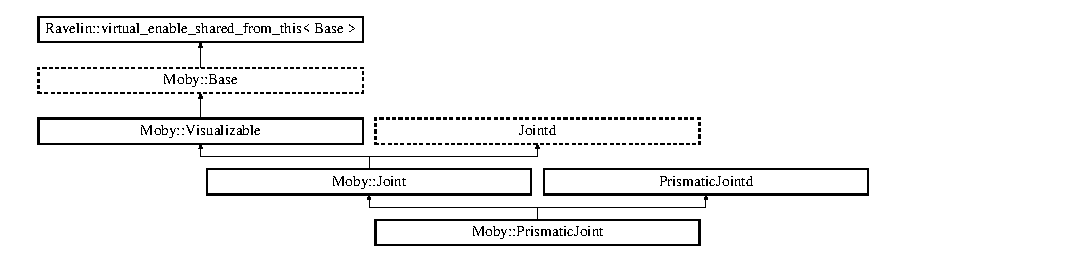
\includegraphics[height=3.070176cm]{classMoby_1_1PrismaticJoint}
\end{center}
\end{figure}
\subsection*{Public Member Functions}
\begin{DoxyCompactItemize}
\item 
{\bf Prismatic\-Joint} ()
\begin{DoxyCompactList}\small\item\em Initializes the joint. \end{DoxyCompactList}\item 
{\bf Prismatic\-Joint} (boost\-::weak\-\_\-ptr$<$ {\bf Rigid\-Body} $>$ inboard, boost\-::weak\-\_\-ptr$<$ {\bf Rigid\-Body} $>$ outboard)
\begin{DoxyCompactList}\small\item\em Initializes the joint with the specified inboard and outboard links. \end{DoxyCompactList}\item 
virtual unsigned {\bfseries num\-\_\-dof} () const \label{classMoby_1_1PrismaticJoint_ad4cf2215b4f41f6f1383ae4635e7c0e4}

\item 
virtual bool {\bfseries is\-\_\-singular\-\_\-config} () const \label{classMoby_1_1PrismaticJoint_a81a0107883c2a688c6c95cb3bbf55a04}

\item 
virtual void {\bfseries evaluate\-\_\-constraints} (double C[$\,$])\label{classMoby_1_1PrismaticJoint_a8b61e8338f4a9d4797b5f7ab65a2dfa5}

\item 
virtual const std\-::vector\\*
$<$ Ravelin\-::\-S\-Velocityd $>$ \& {\bfseries get\-\_\-spatial\-\_\-axes\-\_\-dot} ()\label{classMoby_1_1PrismaticJoint_a3dd12d8f3d283223f107a86583f26f85}

\item 
virtual void {\bfseries determine\-\_\-q} (Ravelin\-::\-Vector\-Nd \&q)\label{classMoby_1_1PrismaticJoint_a498035832680da0091e868c9c52990fa}

\item 
virtual boost\-::shared\-\_\-ptr\\*
$<$ const Ravelin\-::\-Pose3d $>$ {\bfseries get\-\_\-induced\-\_\-pose} ()\label{classMoby_1_1PrismaticJoint_af002260f11d6e4d183db6d6638c31e96}

\item 
virtual void {\bf load\-\_\-from\-\_\-xml} (boost\-::shared\-\_\-ptr$<$ const {\bf X\-M\-L\-Tree} $>$ node, std\-::map$<$ std\-::string, {\bf Base\-Ptr} $>$ \&id\-\_\-map)\label{classMoby_1_1PrismaticJoint_a32fce63f6af0d1508aeb741941f58996}

\begin{DoxyCompactList}\small\item\em Implements \doxyref{Base\-::load\-\_\-from\-\_\-xml()}{p.}{classMoby_1_1Base_a98b861c1d615a748b576aa613f17389f} \end{DoxyCompactList}\item 
virtual void {\bf save\-\_\-to\-\_\-xml} ({\bf X\-M\-L\-Tree\-Ptr} node, std\-::list$<$ boost\-::shared\-\_\-ptr$<$ const {\bf Base} $>$ $>$ \&shared\-\_\-objects) const \label{classMoby_1_1PrismaticJoint_ac5d2ef542aa70f2efe38b59cfade8ced}

\begin{DoxyCompactList}\small\item\em Implements \doxyref{Base\-::save\-\_\-to\-\_\-xml()}{p.}{classMoby_1_1Base_aed64905ca39893d02d1e6c3f03f73aa9} \end{DoxyCompactList}\end{DoxyCompactItemize}
\subsection*{Additional Inherited Members}


\subsection{Detailed Description}
Defines an actuated prismatic joint. 

\begin{DoxyRefDesc}{Todo}
\item[{\bf Todo}]implement a rest position for q? \end{DoxyRefDesc}


\subsection{Constructor \& Destructor Documentation}
\index{Moby\-::\-Prismatic\-Joint@{Moby\-::\-Prismatic\-Joint}!Prismatic\-Joint@{Prismatic\-Joint}}
\index{Prismatic\-Joint@{Prismatic\-Joint}!Moby::PrismaticJoint@{Moby\-::\-Prismatic\-Joint}}
\subsubsection[{Prismatic\-Joint}]{\setlength{\rightskip}{0pt plus 5cm}Prismatic\-Joint\-::\-Prismatic\-Joint (
\begin{DoxyParamCaption}
{}
\end{DoxyParamCaption}
)}\label{classMoby_1_1PrismaticJoint_a8ca0b8c847a3593ec5ffbb21c3b8373b}


Initializes the joint. 

The axis of rotation is set to [0 0 0]. The inboard and outboard links are set to N\-U\-L\-L. 

References Moby\-::\-Joint\-::init\-\_\-data().

\index{Moby\-::\-Prismatic\-Joint@{Moby\-::\-Prismatic\-Joint}!Prismatic\-Joint@{Prismatic\-Joint}}
\index{Prismatic\-Joint@{Prismatic\-Joint}!Moby::PrismaticJoint@{Moby\-::\-Prismatic\-Joint}}
\subsubsection[{Prismatic\-Joint}]{\setlength{\rightskip}{0pt plus 5cm}Prismatic\-Joint\-::\-Prismatic\-Joint (
\begin{DoxyParamCaption}
\item[{boost\-::weak\-\_\-ptr$<$ {\bf Rigid\-Body} $>$}]{inboard, }
\item[{boost\-::weak\-\_\-ptr$<$ {\bf Rigid\-Body} $>$}]{outboard}
\end{DoxyParamCaption}
)}\label{classMoby_1_1PrismaticJoint_a5120edb291a7ea06ffc15cc70417da7b}


Initializes the joint with the specified inboard and outboard links. 

The axis of rotation is set to [0 0 0]. 

The documentation for this class was generated from the following files\-:\begin{DoxyCompactItemize}
\item 
/home/drum/\-Moby/include/\-Moby/Prismatic\-Joint.\-h\item 
/home/drum/\-Moby/src/Prismatic\-Joint.\-cpp\end{DoxyCompactItemize}

\section{Moby\-:\-:R\-C\-Articulated\-Body Class Reference}
\label{classMoby_1_1RCArticulatedBody}\index{Moby\-::\-R\-C\-Articulated\-Body@{Moby\-::\-R\-C\-Articulated\-Body}}


Defines an articulated body for use with reduced-\/coordinate dynamics algorithms.  




{\ttfamily \#include $<$R\-C\-Articulated\-Body.\-h$>$}

Inheritance diagram for Moby\-:\-:R\-C\-Articulated\-Body\-:\begin{figure}[H]
\begin{center}
\leavevmode
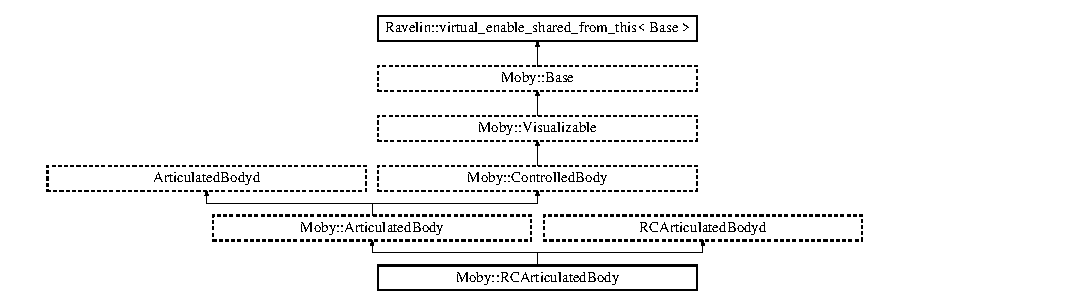
\includegraphics[height=3.684211cm]{classMoby_1_1RCArticulatedBody}
\end{center}
\end{figure}
\subsection*{Public Member Functions}
\begin{DoxyCompactItemize}
\item 
{\bf R\-C\-Articulated\-Body} ()
\begin{DoxyCompactList}\small\item\em Default constructor. \end{DoxyCompactList}\item 
{\bf R\-C\-Articulated\-Body\-Ptr} {\bf clone} () const \label{classMoby_1_1RCArticulatedBody_a87ca0a3a688c4febb29083fa16368f51}

\begin{DoxyCompactList}\small\item\em Clones this. \end{DoxyCompactList}\item 
virtual void {\bf load\-\_\-from\-\_\-xml} (boost\-::shared\-\_\-ptr$<$ const {\bf X\-M\-L\-Tree} $>$ node, std\-::map$<$ std\-::string, {\bf Base\-Ptr} $>$ \&id\-\_\-map)
\begin{DoxyCompactList}\small\item\em Implements \doxyref{Base\-::load\-\_\-from\-\_\-xml()}{p.}{classMoby_1_1Base_a98b861c1d615a748b576aa613f17389f} \end{DoxyCompactList}\item 
virtual void {\bf save\-\_\-to\-\_\-xml} ({\bf X\-M\-L\-Tree\-Ptr} node, std\-::list$<$ boost\-::shared\-\_\-ptr$<$ const {\bf Base} $>$ $>$ \&shared\-\_\-objects) const \label{classMoby_1_1RCArticulatedBody_a08ce8cf881fda06a41bb2323da25f802}

\begin{DoxyCompactList}\small\item\em Implements \doxyref{Base\-::save\-\_\-to\-\_\-xml()}{p.}{classMoby_1_1Base_aed64905ca39893d02d1e6c3f03f73aa9} \end{DoxyCompactList}\item 
virtual void {\bf set\-\_\-links\-\_\-and\-\_\-joints} (const std\-::vector$<$ {\bf Rigid\-Body\-Ptr} $>$ \&links, const std\-::vector$<$ {\bf Joint\-Ptr} $>$ \&joints)\label{classMoby_1_1RCArticulatedBody_a764f142ff0c758d9e49a674ea1206466}

\begin{DoxyCompactList}\small\item\em Sets the vector of links and joints. \end{DoxyCompactList}\item 
virtual void {\bf apply\-\_\-generalized\-\_\-impulse} (const Ravelin\-::\-Shared\-Vector\-Nd \&gj)\label{classMoby_1_1RCArticulatedBody_a620e93f720f7cf69a4bf0d87cfa08640}

\begin{DoxyCompactList}\small\item\em Applies a generalized impulse to the rigid body (calls the simulator) \end{DoxyCompactList}\end{DoxyCompactItemize}
\subsection*{Protected Member Functions}
\begin{DoxyCompactItemize}
\item 
virtual void {\bf compile} ()\label{classMoby_1_1RCArticulatedBody_a4b88af6624948c9e5c74b8ff7ef9e3ca}

\begin{DoxyCompactList}\small\item\em Compiles this body (updates the link transforms and velocities) \end{DoxyCompactList}\end{DoxyCompactItemize}
\subsection*{Additional Inherited Members}


\subsection{Detailed Description}
Defines an articulated body for use with reduced-\/coordinate dynamics algorithms. 

Reduced-\/coordinate articulated bodies cannot rely upon the integrator to automatically update the states (i.\-e., positions, velocities) of the links, as is done with maximal-\/coordinate articulated bodies. Rather, the integrator updates the joint positions and velocities; the states are obtained from this reduced-\/coordinate representation. Notes about concurrency\-: \par
\par


It is generally desirable to be able to run forward dynamics and inverse dynamics algorithms concurrently to simulate actual robotic systems. In general, derived classes should not operate on state variables (joint positions, velocities, accelerations and floating base positions, velocites, and accelerations) directly during execution of the algorithm. Rather, derived classes should operate on copies of the state variables, updating the state variables on conclusion of the algorithms. 

\subsection{Constructor \& Destructor Documentation}
\index{Moby\-::\-R\-C\-Articulated\-Body@{Moby\-::\-R\-C\-Articulated\-Body}!R\-C\-Articulated\-Body@{R\-C\-Articulated\-Body}}
\index{R\-C\-Articulated\-Body@{R\-C\-Articulated\-Body}!Moby::RCArticulatedBody@{Moby\-::\-R\-C\-Articulated\-Body}}
\subsubsection[{R\-C\-Articulated\-Body}]{\setlength{\rightskip}{0pt plus 5cm}R\-C\-Articulated\-Body\-::\-R\-C\-Articulated\-Body (
\begin{DoxyParamCaption}
{}
\end{DoxyParamCaption}
)}\label{classMoby_1_1RCArticulatedBody_add3181d88841c6ea6d3c132be9be8085}


Default constructor. 

Constructs a reduced-\/coordinate articulated body with no joints and no links. 

\subsection{Member Function Documentation}
\index{Moby\-::\-R\-C\-Articulated\-Body@{Moby\-::\-R\-C\-Articulated\-Body}!load\-\_\-from\-\_\-xml@{load\-\_\-from\-\_\-xml}}
\index{load\-\_\-from\-\_\-xml@{load\-\_\-from\-\_\-xml}!Moby::RCArticulatedBody@{Moby\-::\-R\-C\-Articulated\-Body}}
\subsubsection[{load\-\_\-from\-\_\-xml}]{\setlength{\rightskip}{0pt plus 5cm}void R\-C\-Articulated\-Body\-::load\-\_\-from\-\_\-xml (
\begin{DoxyParamCaption}
\item[{boost\-::shared\-\_\-ptr$<$ const {\bf X\-M\-L\-Tree} $>$}]{node, }
\item[{std\-::map$<$ std\-::string, {\bf Base\-Ptr} $>$ \&}]{id\-\_\-map}
\end{DoxyParamCaption}
)\hspace{0.3cm}{\ttfamily [virtual]}}\label{classMoby_1_1RCArticulatedBody_a8e694464f29ac406b4b9ecef5e0d8bac}


Implements \doxyref{Base\-::load\-\_\-from\-\_\-xml()}{p.}{classMoby_1_1Base_a98b861c1d615a748b576aa613f17389f} 

\begin{DoxyPrecond}{Precondition}
all links and joints must be loaded using their respective serialization methods before this method is called 
\end{DoxyPrecond}


Reimplemented from {\bf Moby\-::\-Articulated\-Body} \doxyref{}{p.}{classMoby_1_1ArticulatedBody_a7d86b8e81bee372ba5cd5de35ccfde59}.



References Moby\-::\-X\-M\-L\-Attrib\-::get\-\_\-bool\-\_\-value(), Moby\-::\-X\-M\-L\-Attrib\-::get\-\_\-origin\-\_\-value(), and Moby\-::\-X\-M\-L\-Attrib\-::get\-\_\-rpy\-\_\-value().



The documentation for this class was generated from the following files\-:\begin{DoxyCompactItemize}
\item 
/home/drum/\-Moby/include/\-Moby/R\-C\-Articulated\-Body.\-h\item 
/home/drum/\-Moby/src/R\-C\-Articulated\-Body.\-cpp\end{DoxyCompactItemize}

\section{Moby\-:\-:R\-C\-Articulated\-Body\-Inv\-Dyn\-Algo Class Reference}
\label{classMoby_1_1RCArticulatedBodyInvDynAlgo}\index{Moby\-::\-R\-C\-Articulated\-Body\-Inv\-Dyn\-Algo@{Moby\-::\-R\-C\-Articulated\-Body\-Inv\-Dyn\-Algo}}


Abstract class for performing inverse dynamics computation on a reduced-\/coordinate articulatedc body.  




{\ttfamily \#include $<$R\-C\-Articulated\-Body\-Inv\-Dyn\-Algo.\-h$>$}

Inheritance diagram for Moby\-:\-:R\-C\-Articulated\-Body\-Inv\-Dyn\-Algo\-:\begin{figure}[H]
\begin{center}
\leavevmode
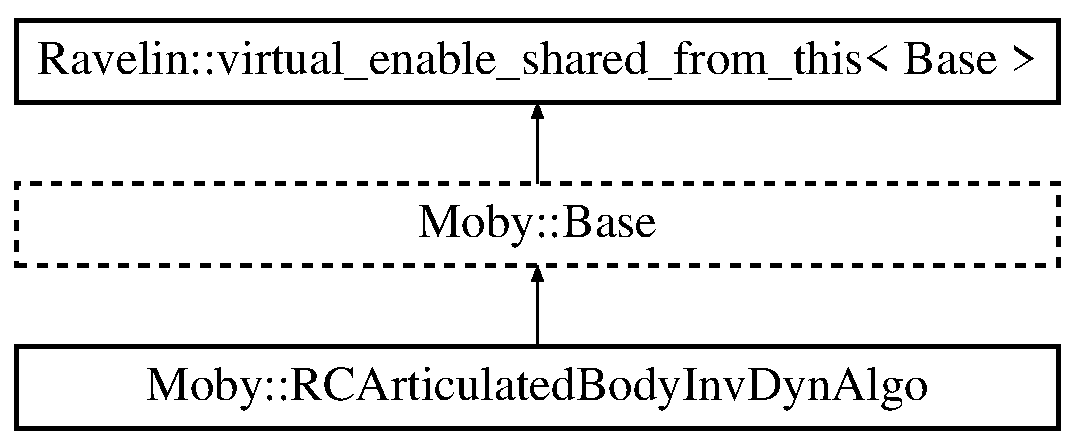
\includegraphics[height=3.000000cm]{classMoby_1_1RCArticulatedBodyInvDynAlgo}
\end{center}
\end{figure}
\subsection*{Public Member Functions}
\begin{DoxyCompactItemize}
\item 
virtual std\-::map\\*
$<$ boost\-::shared\-\_\-ptr$<$ {\bf Joint} $>$\\*
, Ravelin\-::\-Vector\-Nd $>$ {\bf calc\-\_\-inv\-\_\-dyn} (boost\-::shared\-\_\-ptr$<$ {\bf R\-C\-Articulated\-Body} $>$ body, const std\-::map$<$ boost\-::shared\-\_\-ptr$<$ {\bf Rigid\-Body} $>$, {\bf R\-C\-Articulated\-Body\-Inv\-Dyn\-Data} $>$ \&inv\-\_\-dyn\-\_\-data)=0
\begin{DoxyCompactList}\small\item\em Classes must implement the method below. \end{DoxyCompactList}\end{DoxyCompactItemize}
\subsection*{Additional Inherited Members}


\subsection{Detailed Description}
Abstract class for performing inverse dynamics computation on a reduced-\/coordinate articulatedc body. 

\subsection{Member Function Documentation}
\index{Moby\-::\-R\-C\-Articulated\-Body\-Inv\-Dyn\-Algo@{Moby\-::\-R\-C\-Articulated\-Body\-Inv\-Dyn\-Algo}!calc\-\_\-inv\-\_\-dyn@{calc\-\_\-inv\-\_\-dyn}}
\index{calc\-\_\-inv\-\_\-dyn@{calc\-\_\-inv\-\_\-dyn}!Moby::RCArticulatedBodyInvDynAlgo@{Moby\-::\-R\-C\-Articulated\-Body\-Inv\-Dyn\-Algo}}
\subsubsection[{calc\-\_\-inv\-\_\-dyn}]{\setlength{\rightskip}{0pt plus 5cm}virtual std\-::map$<$boost\-::shared\-\_\-ptr$<${\bf Joint}$>$, Ravelin\-::\-Vector\-Nd$>$ Moby\-::\-R\-C\-Articulated\-Body\-Inv\-Dyn\-Algo\-::calc\-\_\-inv\-\_\-dyn (
\begin{DoxyParamCaption}
\item[{boost\-::shared\-\_\-ptr$<$ {\bf R\-C\-Articulated\-Body} $>$}]{body, }
\item[{const std\-::map$<$ boost\-::shared\-\_\-ptr$<$ {\bf Rigid\-Body} $>$, {\bf R\-C\-Articulated\-Body\-Inv\-Dyn\-Data} $>$ \&}]{inv\-\_\-dyn\-\_\-data}
\end{DoxyParamCaption}
)\hspace{0.3cm}{\ttfamily [pure virtual]}}\label{classMoby_1_1RCArticulatedBodyInvDynAlgo_acb5f5edb8cb4ed336570c7519350ad9a}


Classes must implement the method below. 

Given the current base position and velocity, the joint positions and joint velocities, the external forces on all links (including the base), and the desired joint and base accelerations, the inverse dynamics method must compute the forces applied to the joint actuators to achieve these accelerations. \begin{DoxyReturn}{Returns}
a map from joints to computed actuator forces 
\end{DoxyReturn}


The documentation for this class was generated from the following file\-:\begin{DoxyCompactItemize}
\item 
/home/drum/\-Moby/include/\-Moby/R\-C\-Articulated\-Body\-Inv\-Dyn\-Algo.\-h\end{DoxyCompactItemize}

\section{Moby\-:\-:R\-C\-Articulated\-Body\-Inv\-Dyn\-Data Class Reference}
\label{classMoby_1_1RCArticulatedBodyInvDynData}\index{Moby\-::\-R\-C\-Articulated\-Body\-Inv\-Dyn\-Data@{Moby\-::\-R\-C\-Articulated\-Body\-Inv\-Dyn\-Data}}


Wrapper class for passing data to and from inverse dynamics algorithms.  




{\ttfamily \#include $<$R\-C\-Articulated\-Body\-Inv\-Dyn\-Algo.\-h$>$}

\subsection*{Public Attributes}
\begin{DoxyCompactItemize}
\item 
Ravelin\-::\-S\-Forced {\bf wext}\label{classMoby_1_1RCArticulatedBodyInvDynData_ae9364585293b12472b1ea9f95cffa1de}

\begin{DoxyCompactList}\small\item\em External force applied to this link. \end{DoxyCompactList}\item 
Ravelin\-::\-Vector\-Nd {\bf qdd}\label{classMoby_1_1RCArticulatedBodyInvDynData_a258a1da2fbd02c1b4aae0b5ac1a4c6ea}

\begin{DoxyCompactList}\small\item\em Inner joint acceleration (desired) \end{DoxyCompactList}\end{DoxyCompactItemize}


\subsection{Detailed Description}
Wrapper class for passing data to and from inverse dynamics algorithms. 

The documentation for this class was generated from the following file\-:\begin{DoxyCompactItemize}
\item 
/home/drum/\-Moby/include/\-Moby/R\-C\-Articulated\-Body\-Inv\-Dyn\-Algo.\-h\end{DoxyCompactItemize}

\section{Moby\-:\-:Recurrent\-Force Class Reference}
\label{classMoby_1_1RecurrentForce}\index{Moby\-::\-Recurrent\-Force@{Moby\-::\-Recurrent\-Force}}


Used for applying forces to the simulation on every time step.  




{\ttfamily \#include $<$Recurrent\-Force.\-h$>$}

Inheritance diagram for Moby\-:\-:Recurrent\-Force\-:\begin{figure}[H]
\begin{center}
\leavevmode
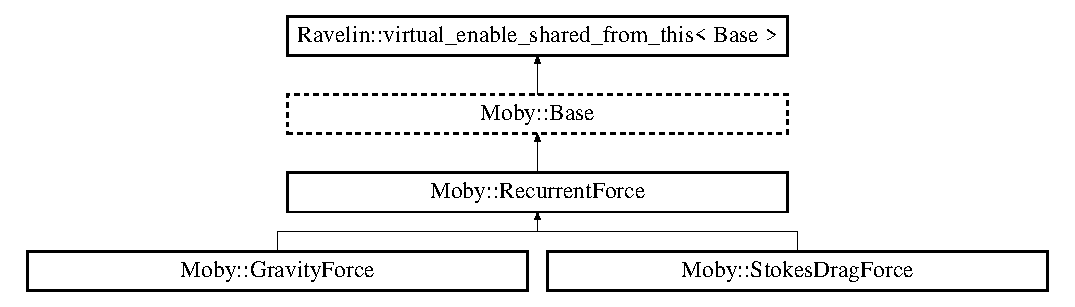
\includegraphics[height=3.684211cm]{classMoby_1_1RecurrentForce}
\end{center}
\end{figure}
\subsection*{Public Member Functions}
\begin{DoxyCompactItemize}
\item 
virtual void {\bf add\-\_\-force} (boost\-::shared\-\_\-ptr$<$ Ravelin\-::\-Dynamic\-Bodyd $>$ body)=0\label{classMoby_1_1RecurrentForce_a51481753177921d9896e3bfa04c24724}

\begin{DoxyCompactList}\small\item\em Abstract method for applying this force/torque to a body. \end{DoxyCompactList}\end{DoxyCompactItemize}
\subsection*{Additional Inherited Members}


\subsection{Detailed Description}
Used for applying forces to the simulation on every time step. 

Recurrent forces may be constant (like gravity) or vary by the velocity of the body (like wind resistance). The recurrent force can be either an actual force, or a torque, or both. 

The documentation for this class was generated from the following file\-:\begin{DoxyCompactItemize}
\item 
/home/drum/\-Moby/include/\-Moby/Recurrent\-Force.\-h\end{DoxyCompactItemize}

\section{Moby\-:\-:Revolute\-Joint Class Reference}
\label{classMoby_1_1RevoluteJoint}\index{Moby\-::\-Revolute\-Joint@{Moby\-::\-Revolute\-Joint}}


Defines an actuated revolute joint.  




{\ttfamily \#include $<$Revolute\-Joint.\-h$>$}

Inheritance diagram for Moby\-:\-:Revolute\-Joint\-:\begin{figure}[H]
\begin{center}
\leavevmode
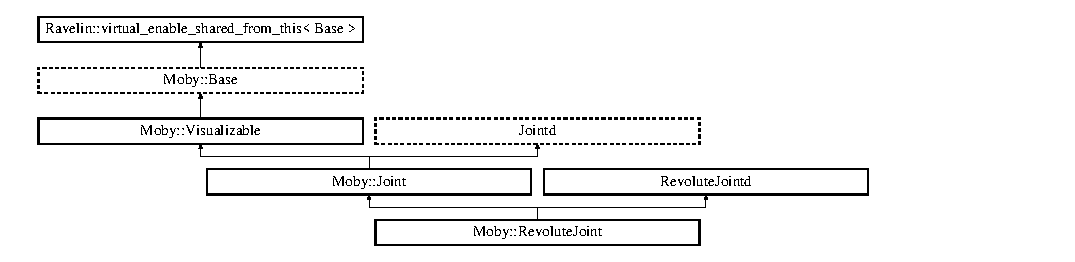
\includegraphics[height=3.070176cm]{classMoby_1_1RevoluteJoint}
\end{center}
\end{figure}
\subsection*{Public Member Functions}
\begin{DoxyCompactItemize}
\item 
{\bf Revolute\-Joint} ()
\begin{DoxyCompactList}\small\item\em Initializes the joint. \end{DoxyCompactList}\item 
{\bf Revolute\-Joint} (boost\-::weak\-\_\-ptr$<$ {\bf Rigid\-Body} $>$ inboard, boost\-::weak\-\_\-ptr$<$ {\bf Rigid\-Body} $>$ outboard)
\begin{DoxyCompactList}\small\item\em Initializes the joint with the specified inboard and outboard links. \end{DoxyCompactList}\item 
virtual unsigned {\bfseries num\-\_\-dof} () const \label{classMoby_1_1RevoluteJoint_ab0b80e92ddf0b9726d48c6ec73470ea5}

\item 
virtual bool {\bfseries is\-\_\-singular\-\_\-config} () const \label{classMoby_1_1RevoluteJoint_a4be56bf8fbf338cff6c4354220e9f99b}

\item 
virtual void {\bfseries evaluate\-\_\-constraints} (double C[$\,$])\label{classMoby_1_1RevoluteJoint_a555e5b5ef08d7598b5c59c973a0e3fb9}

\item 
virtual const std\-::vector\\*
$<$ Ravelin\-::\-S\-Velocityd $>$ \& {\bfseries get\-\_\-spatial\-\_\-axes\-\_\-dot} ()\label{classMoby_1_1RevoluteJoint_a42c7b2a5e37860c3c0cc96f76a10efbe}

\item 
virtual void {\bfseries determine\-\_\-q} (Ravelin\-::\-Vector\-Nd \&q)\label{classMoby_1_1RevoluteJoint_a8035f5b87dd890e55cf4bcbab321e3dd}

\item 
virtual boost\-::shared\-\_\-ptr\\*
$<$ const Ravelin\-::\-Pose3d $>$ {\bfseries get\-\_\-induced\-\_\-pose} ()\label{classMoby_1_1RevoluteJoint_ab13d9a0845aa59083792f23aac5c174d}

\item 
virtual void {\bf load\-\_\-from\-\_\-xml} (boost\-::shared\-\_\-ptr$<$ const {\bf X\-M\-L\-Tree} $>$ node, std\-::map$<$ std\-::string, {\bf Base\-Ptr} $>$ \&id\-\_\-map)\label{classMoby_1_1RevoluteJoint_af72df350d32e71d76b3505f29a633cce}

\begin{DoxyCompactList}\small\item\em Implements \doxyref{Base\-::load\-\_\-from\-\_\-xml()}{p.}{classMoby_1_1Base_a98b861c1d615a748b576aa613f17389f} \end{DoxyCompactList}\item 
virtual void {\bf save\-\_\-to\-\_\-xml} ({\bf X\-M\-L\-Tree\-Ptr} node, std\-::list$<$ boost\-::shared\-\_\-ptr$<$ const {\bf Base} $>$ $>$ \&shared\-\_\-objects) const \label{classMoby_1_1RevoluteJoint_a97b43695c74e98937997e30f71b3b26d}

\begin{DoxyCompactList}\small\item\em Implements \doxyref{Base\-::save\-\_\-to\-\_\-xml()}{p.}{classMoby_1_1Base_aed64905ca39893d02d1e6c3f03f73aa9} \end{DoxyCompactList}\end{DoxyCompactItemize}
\subsection*{Additional Inherited Members}


\subsection{Detailed Description}
Defines an actuated revolute joint. 

\subsection{Constructor \& Destructor Documentation}
\index{Moby\-::\-Revolute\-Joint@{Moby\-::\-Revolute\-Joint}!Revolute\-Joint@{Revolute\-Joint}}
\index{Revolute\-Joint@{Revolute\-Joint}!Moby::RevoluteJoint@{Moby\-::\-Revolute\-Joint}}
\subsubsection[{Revolute\-Joint}]{\setlength{\rightskip}{0pt plus 5cm}Revolute\-Joint\-::\-Revolute\-Joint (
\begin{DoxyParamCaption}
{}
\end{DoxyParamCaption}
)}\label{classMoby_1_1RevoluteJoint_aa36d84d49ebe6bed2aaf93cc1de46a84}


Initializes the joint. 

The axis of rotation is set to [0 0 0]. The inboard and outboard links are set to N\-U\-L\-L. 

References Moby\-::\-Joint\-::init\-\_\-data().

\index{Moby\-::\-Revolute\-Joint@{Moby\-::\-Revolute\-Joint}!Revolute\-Joint@{Revolute\-Joint}}
\index{Revolute\-Joint@{Revolute\-Joint}!Moby::RevoluteJoint@{Moby\-::\-Revolute\-Joint}}
\subsubsection[{Revolute\-Joint}]{\setlength{\rightskip}{0pt plus 5cm}Revolute\-Joint\-::\-Revolute\-Joint (
\begin{DoxyParamCaption}
\item[{boost\-::weak\-\_\-ptr$<$ {\bf Rigid\-Body} $>$}]{inboard, }
\item[{boost\-::weak\-\_\-ptr$<$ {\bf Rigid\-Body} $>$}]{outboard}
\end{DoxyParamCaption}
)}\label{classMoby_1_1RevoluteJoint_a6d20f72ec980aa64f2731ef055d2e0e6}


Initializes the joint with the specified inboard and outboard links. 

The axis of rotation is set to [0 0 0]. 

The documentation for this class was generated from the following files\-:\begin{DoxyCompactItemize}
\item 
/home/drum/\-Moby/include/\-Moby/Revolute\-Joint.\-h\item 
/home/drum/\-Moby/src/Revolute\-Joint.\-cpp\end{DoxyCompactItemize}

\section{Moby\-:\-:Rigid\-Body Class Reference}
\label{classMoby_1_1RigidBody}\index{Moby\-::\-Rigid\-Body@{Moby\-::\-Rigid\-Body}}


Represents a single rigid body.  




{\ttfamily \#include $<$Rigid\-Body.\-h$>$}

Inheritance diagram for Moby\-:\-:Rigid\-Body\-:\begin{figure}[H]
\begin{center}
\leavevmode
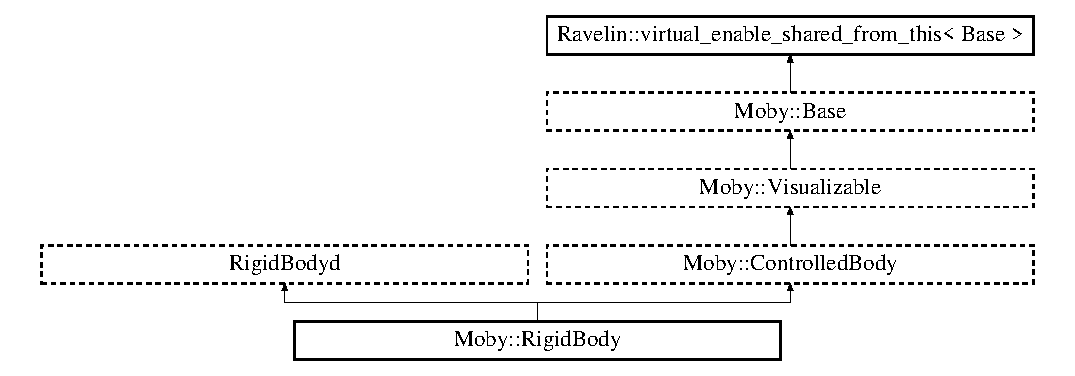
\includegraphics[height=4.605263cm]{classMoby_1_1RigidBody}
\end{center}
\end{figure}
\subsection*{Public Types}
\begin{DoxyCompactItemize}
\item 
enum {\bfseries Compliance} \{ {\bfseries e\-Rigid}, 
{\bfseries e\-Compliant}
 \}
\end{DoxyCompactItemize}
\subsection*{Public Member Functions}
\begin{DoxyCompactItemize}
\item 
{\bf Rigid\-Body} ()
\begin{DoxyCompactList}\small\item\em Default constructor. \end{DoxyCompactList}\item 
virtual void {\bf set\-\_\-visualization\-\_\-data} (osg\-::\-Node $\ast$vdata)\label{classMoby_1_1RigidBody_aa920d8cc52cd38f7282b4c192a57ed08}

\begin{DoxyCompactList}\small\item\em Sets the visualization data from a node. \end{DoxyCompactList}\item 
virtual void {\bf load\-\_\-from\-\_\-xml} (boost\-::shared\-\_\-ptr$<$ const {\bf X\-M\-L\-Tree} $>$ node, std\-::map$<$ std\-::string, {\bf Base\-Ptr} $>$ \&id\-\_\-map)\label{classMoby_1_1RigidBody_a26bee5f435e488d8048e0b827ee91004}

\begin{DoxyCompactList}\small\item\em Implements \doxyref{Base\-::load\-\_\-from\-\_\-xml()}{p.}{classMoby_1_1Base_a98b861c1d615a748b576aa613f17389f} \end{DoxyCompactList}\item 
virtual void {\bf save\-\_\-to\-\_\-xml} ({\bf X\-M\-L\-Tree\-Ptr} node, std\-::list$<$ boost\-::shared\-\_\-ptr$<$ const {\bf Base} $>$ $>$ \&shared\-\_\-objects) const \label{classMoby_1_1RigidBody_a071ed106863e0cd018b5ccf3bce5f5e2}

\begin{DoxyCompactList}\small\item\em Implements \doxyref{Base\-::save\-\_\-to\-\_\-xml()}{p.}{classMoby_1_1Base_aed64905ca39893d02d1e6c3f03f73aa9} \end{DoxyCompactList}\item 
bool {\bf is\-\_\-child\-\_\-link} (boost\-::shared\-\_\-ptr$<$ const {\bf Rigid\-Body} $>$ query) const \label{classMoby_1_1RigidBody_a7907871ed17117ec16d59de2a0932ff0}

\begin{DoxyCompactList}\small\item\em Determines whether the given link is a child link of this. \end{DoxyCompactList}\item 
bool {\bf is\-\_\-descendant\-\_\-link} (boost\-::shared\-\_\-ptr$<$ const {\bf Rigid\-Body} $>$ query) const 
\begin{DoxyCompactList}\small\item\em Determines whether the given link is a descendant of this. \end{DoxyCompactList}\item 
{\bf Rigid\-Body\-Ptr} {\bf get\-\_\-parent\-\_\-link} () const \label{classMoby_1_1RigidBody_aef849d722736091bde943426f72b2f65}

\begin{DoxyCompactList}\small\item\em Gets the first parent link of this link; returns N\-U\-L\-L if there is no parent. \end{DoxyCompactList}\item 
{\bf Joint\-Ptr} {\bf get\-\_\-inner\-\_\-joint\-\_\-explicit} () const 
\begin{DoxyCompactList}\small\item\em Gets the explicit inner joint of this link; returns N\-U\-L\-L if there is no explicit inner joint. \end{DoxyCompactList}\item 
virtual void {\bf prepare\-\_\-to\-\_\-calc\-\_\-ode} (Ravelin\-::\-Shared\-Const\-Vector\-Nd \&x, double t, double dt, void $\ast$data)\label{classMoby_1_1RigidBody_ab39581c787c03702e3c38186625890dc}

\begin{DoxyCompactList}\small\item\em Prepares to compute the O\-D\-E. \end{DoxyCompactList}\item 
virtual void {\bf prepare\-\_\-to\-\_\-calc\-\_\-ode\-\_\-sustained\-\_\-constraints} (Ravelin\-::\-Shared\-Const\-Vector\-Nd \&x, double t, double dt, void $\ast$data)\label{classMoby_1_1RigidBody_a34766f49520ffd4fa25e1b148ac7df15}

\begin{DoxyCompactList}\small\item\em Prepares to compute the derivative of the body (sustained constraints) \end{DoxyCompactList}\item 
virtual void {\bf ode} (double t, double dt, void $\ast$data, Ravelin\-::\-Shared\-Vector\-Nd \&dx)\label{classMoby_1_1RigidBody_add1c713a00195f49a20196ae4196c8b6}

\begin{DoxyCompactList}\small\item\em Computes the O\-D\-E. \end{DoxyCompactList}\item 
virtual void {\bf set\-\_\-articulated\-\_\-body} (boost\-::shared\-\_\-ptr$<$ {\bf Articulated\-Body} $>$ body)
\begin{DoxyCompactList}\small\item\em Sets the articulated body corresponding to this body. \end{DoxyCompactList}\item 
virtual void {\bf set\-\_\-inertia} (const Ravelin\-::\-Spatial\-R\-B\-Inertiad \&J)\label{classMoby_1_1RigidBody_a95342ceec35b4ed59270acb3152201da}

\begin{DoxyCompactList}\small\item\em Sets the rigid body inertia for this body. \end{DoxyCompactList}\item 
virtual void {\bf apply\-\_\-generalized\-\_\-impulse} (const Ravelin\-::\-Shared\-Vector\-Nd \&gj)\label{classMoby_1_1RigidBody_a143af073f492eca104c916554b4d2b8d}

\begin{DoxyCompactList}\small\item\em Applies a generalized impulse to the rigid body (calls the simulator) \end{DoxyCompactList}\item 
{\footnotesize template$<$class Output\-Iterator $>$ }\\Output\-Iterator {\bfseries get\-\_\-parent\-\_\-links} (Output\-Iterator begin) const \label{classMoby_1_1RigidBody_a1bccd0004208c2f4fdad476616f10b67}

\item 
{\footnotesize template$<$class Output\-Iterator $>$ }\\Output\-Iterator {\bfseries get\-\_\-child\-\_\-links} (Output\-Iterator begin) const \label{classMoby_1_1RigidBody_a4361f780f430975b6a7db6aa845f5af5}

\item 
{\footnotesize template$<$class Output\-Iterator $>$ }\\Output\-Iterator {\bfseries get\-\_\-parent\-\_\-links} (Output\-Iterator begin) const \label{classMoby_1_1RigidBody_a1bccd0004208c2f4fdad476616f10b67}

\item 
{\footnotesize template$<$class Output\-Iterator $>$ }\\Output\-Iterator {\bfseries get\-\_\-child\-\_\-links} (Output\-Iterator begin) const \label{classMoby_1_1RigidBody_a4361f780f430975b6a7db6aa845f5af5}

\end{DoxyCompactItemize}
\subsection*{Public Attributes}
\begin{DoxyCompactItemize}
\item 
std\-::list$<$ {\bf Collision\-Geometry\-Ptr} $>$ {\bf geometries}\label{classMoby_1_1RigidBody_add39aaa78b528ce6af4f3c2c8c491787}

\begin{DoxyCompactList}\small\item\em Collision geometries, if any, for this rigid body. \end{DoxyCompactList}\item 
Compliance {\bf compliance}\label{classMoby_1_1RigidBody_a8a6469c96b4c444dcebb50c8c86f4915}

\begin{DoxyCompactList}\small\item\em Compliance value, determines event type. \end{DoxyCompactList}\end{DoxyCompactItemize}
\subsection*{Friends}
\begin{DoxyCompactItemize}
\item 
class {\bfseries Articulated\-Body}\label{classMoby_1_1RigidBody_a7d29a1ee423a6e8dab5bf1a58b001f17}

\item 
class {\bfseries R\-C\-Articulated\-Body}\label{classMoby_1_1RigidBody_af04ff9fbc4b43045d831b0922dfad60c}

\item 
class {\bfseries M\-C\-Articulated\-Body}\label{classMoby_1_1RigidBody_a8671e4c6b33a082e8cbbc13466bdd6f4}

\item 
class {\bfseries Time\-Stepping\-Simulator}\label{classMoby_1_1RigidBody_a9a45dd70a5ca67a83fe0954e77276589}

\item 
class {\bfseries Joint}\label{classMoby_1_1RigidBody_a2b27269e818d7b63995be0e0f812bf54}

\end{DoxyCompactItemize}
\subsection*{Additional Inherited Members}


\subsection{Detailed Description}
Represents a single rigid body. 

Contains information needed to represent a rigid body, including position and velocity (both linear and angular), mass, center of mass, inertia matrix, collision data, and visualization data. This class is used for both non-\/articulated and articulated rigid bodies, though not all member data may be used in the latter. \begin{DoxyRefDesc}{Todo}
\item[{\bf Todo}]implement rest matrix \end{DoxyRefDesc}


\subsection{Constructor \& Destructor Documentation}
\index{Moby\-::\-Rigid\-Body@{Moby\-::\-Rigid\-Body}!Rigid\-Body@{Rigid\-Body}}
\index{Rigid\-Body@{Rigid\-Body}!Moby::RigidBody@{Moby\-::\-Rigid\-Body}}
\subsubsection[{Rigid\-Body}]{\setlength{\rightskip}{0pt plus 5cm}Rigid\-Body\-::\-Rigid\-Body (
\begin{DoxyParamCaption}
{}
\end{DoxyParamCaption}
)}\label{classMoby_1_1RigidBody_a28203d38d278da0695ace20c66ee5f0a}


Default constructor. 

Constructs a rigid body with zero mass, zero inertia tensor, and center of mass at [0,0,0] with position at [0,0,0], identity orientation, and zero linear and angular velocity. Body is enabled by default. 

\subsection{Member Function Documentation}
\index{Moby\-::\-Rigid\-Body@{Moby\-::\-Rigid\-Body}!get\-\_\-inner\-\_\-joint\-\_\-explicit@{get\-\_\-inner\-\_\-joint\-\_\-explicit}}
\index{get\-\_\-inner\-\_\-joint\-\_\-explicit@{get\-\_\-inner\-\_\-joint\-\_\-explicit}!Moby::RigidBody@{Moby\-::\-Rigid\-Body}}
\subsubsection[{get\-\_\-inner\-\_\-joint\-\_\-explicit}]{\setlength{\rightskip}{0pt plus 5cm}{\bf Joint\-Ptr} Rigid\-Body\-::get\-\_\-inner\-\_\-joint\-\_\-explicit (
\begin{DoxyParamCaption}
{}
\end{DoxyParamCaption}
) const}\label{classMoby_1_1RigidBody_af1e9ffb4be18421ac010d7c41666b567}


Gets the explicit inner joint of this link; returns N\-U\-L\-L if there is no explicit inner joint. 

Throws an exception if this link has multiple explicit inner joints \index{Moby\-::\-Rigid\-Body@{Moby\-::\-Rigid\-Body}!is\-\_\-descendant\-\_\-link@{is\-\_\-descendant\-\_\-link}}
\index{is\-\_\-descendant\-\_\-link@{is\-\_\-descendant\-\_\-link}!Moby::RigidBody@{Moby\-::\-Rigid\-Body}}
\subsubsection[{is\-\_\-descendant\-\_\-link}]{\setlength{\rightskip}{0pt plus 5cm}bool Rigid\-Body\-::is\-\_\-descendant\-\_\-link (
\begin{DoxyParamCaption}
\item[{boost\-::shared\-\_\-ptr$<$ const {\bf Rigid\-Body} $>$}]{query}
\end{DoxyParamCaption}
) const}\label{classMoby_1_1RigidBody_ae488e06d52ec66cd4a7d170e7654717a}


Determines whether the given link is a descendant of this. 

\begin{DoxyNote}{Note}
returns {\bfseries true} if query == this 
\end{DoxyNote}
\index{Moby\-::\-Rigid\-Body@{Moby\-::\-Rigid\-Body}!set\-\_\-articulated\-\_\-body@{set\-\_\-articulated\-\_\-body}}
\index{set\-\_\-articulated\-\_\-body@{set\-\_\-articulated\-\_\-body}!Moby::RigidBody@{Moby\-::\-Rigid\-Body}}
\subsubsection[{set\-\_\-articulated\-\_\-body}]{\setlength{\rightskip}{0pt plus 5cm}void Rigid\-Body\-::set\-\_\-articulated\-\_\-body (
\begin{DoxyParamCaption}
\item[{boost\-::shared\-\_\-ptr$<$ {\bf Articulated\-Body} $>$}]{body}
\end{DoxyParamCaption}
)\hspace{0.3cm}{\ttfamily [virtual]}}\label{classMoby_1_1RigidBody_a49d971ac0c958ec133df664008b8af21}


Sets the articulated body corresponding to this body. 


\begin{DoxyParams}{Parameters}
{\em body} & a pointer to the articulated body or N\-U\-L\-L if this body is not a link in an articulated body \\
\hline
\end{DoxyParams}


The documentation for this class was generated from the following files\-:\begin{DoxyCompactItemize}
\item 
/home/drum/\-Moby/include/\-Moby/Rigid\-Body.\-h\item 
/home/drum/\-Moby/include/\-Moby/Rigid\-Body.\-inl\item 
/home/drum/\-Moby/src/Rigid\-Body.\-cpp\end{DoxyCompactItemize}

\section{Moby\-:\-:Screw\-Joint Class Reference}
\label{classMoby_1_1ScrewJoint}\index{Moby\-::\-Screw\-Joint@{Moby\-::\-Screw\-Joint}}


Defines an actuated screw (helical) joint.  




{\ttfamily \#include $<$Screw\-Joint.\-h$>$}

Inheritance diagram for Moby\-:\-:Screw\-Joint\-:\begin{figure}[H]
\begin{center}
\leavevmode
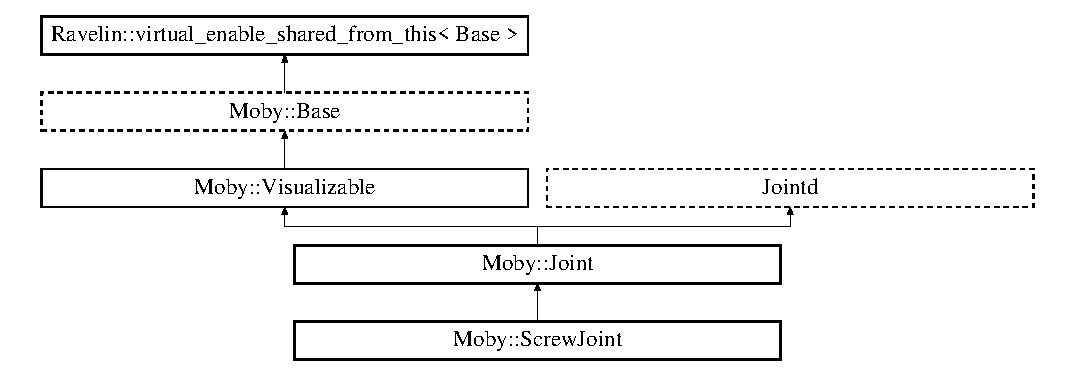
\includegraphics[height=4.605263cm]{classMoby_1_1ScrewJoint}
\end{center}
\end{figure}
\subsection*{Public Member Functions}
\begin{DoxyCompactItemize}
\item 
{\bf Screw\-Joint} ()
\begin{DoxyCompactList}\small\item\em Initializes the joint. \end{DoxyCompactList}\item 
{\bf Screw\-Joint} (boost\-::weak\-\_\-ptr$<$ {\bf Rigid\-Body} $>$ inboard, boost\-::weak\-\_\-ptr$<$ {\bf Rigid\-Body} $>$ outboard)
\begin{DoxyCompactList}\small\item\em Initializes the joint with the specified inboard and outboard links. \end{DoxyCompactList}\item 
const Ravelin\-::\-Vector3d \& {\bfseries get\-\_\-axis} () const \label{classMoby_1_1ScrewJoint_ad1aecf6b9694eef1ef200dcc5f4dd600}

\item 
void {\bf set\-\_\-axis} (const Ravelin\-::\-Vector3d \&axis)
\begin{DoxyCompactList}\small\item\em Sets the global axis for this joint. \end{DoxyCompactList}\item 
virtual void {\bf update\-\_\-spatial\-\_\-axes} ()\label{classMoby_1_1ScrewJoint_a698fdfee9b94db32a7e5b75a8bcc49bb}

\begin{DoxyCompactList}\small\item\em Updates the spatial axis for this joint. \end{DoxyCompactList}\item 
virtual void {\bf determine\-\_\-q} (Vector\-N \&q)\label{classMoby_1_1ScrewJoint_a9570aa8c5471c8c36cc65905925b5db5}

\begin{DoxyCompactList}\small\item\em Determines (and sets) the value of Q from the axis and the inboard link and outboard link transforms. \end{DoxyCompactList}\item 
virtual boost\-::shared\-\_\-ptr\\*
$<$ const Ravelin\-::\-Pose3d $>$ \& {\bf get\-\_\-induced\-\_\-pose} ()\label{classMoby_1_1ScrewJoint_a6902884b5cf370f78508d7e59ad16740}

\begin{DoxyCompactList}\small\item\em Gets the (local) transform for this joint. \end{DoxyCompactList}\item 
virtual const std\-::vector\\*
$<$ Ravelin\-::\-S\-Velocityd $>$ \& {\bf get\-\_\-spatial\-\_\-axes\-\_\-dot} ()\label{classMoby_1_1ScrewJoint_ad47c2af36fe8372836aed65aecd309da}

\begin{DoxyCompactList}\small\item\em Gets the derivative for the spatial axes for this joint. \end{DoxyCompactList}\item 
virtual void {\bf load\-\_\-from\-\_\-xml} (boost\-::shared\-\_\-ptr$<$ const {\bf X\-M\-L\-Tree} $>$ node, std\-::map$<$ std\-::string, {\bf Base\-Ptr} $>$ \&id\-\_\-map)\label{classMoby_1_1ScrewJoint_a6fd5ddb252a077e791697bc90718ab5d}

\begin{DoxyCompactList}\small\item\em Implements \doxyref{Base\-::load\-\_\-from\-\_\-xml()}{p.}{classMoby_1_1Base_a98b861c1d615a748b576aa613f17389f} \end{DoxyCompactList}\item 
virtual void {\bf save\-\_\-to\-\_\-xml} ({\bf X\-M\-L\-Tree\-Ptr} node, std\-::list$<$ boost\-::shared\-\_\-ptr$<$ const {\bf Base} $>$ $>$ \&shared\-\_\-objects) const \label{classMoby_1_1ScrewJoint_a3310bc567f4fa3a82bae87d5d35dcffb}

\begin{DoxyCompactList}\small\item\em Implements \doxyref{Base\-::save\-\_\-to\-\_\-xml()}{p.}{classMoby_1_1Base_aed64905ca39893d02d1e6c3f03f73aa9} \end{DoxyCompactList}\item 
virtual unsigned {\bfseries num\-\_\-dof} () const \label{classMoby_1_1ScrewJoint_a370cdad1db58c8c537161c034884d51f}

\item 
virtual void {\bf evaluate\-\_\-constraints} (double C[$\,$])\label{classMoby_1_1ScrewJoint_ad9057164b54e8860957e3bdeda08e788}

\begin{DoxyCompactList}\small\item\em Evaluates the constraint equations. \end{DoxyCompactList}\item 
double {\bf get\-\_\-pitch} () const \label{classMoby_1_1ScrewJoint_af912552d21c87c02c62adc4edfdf95d6}

\begin{DoxyCompactList}\small\item\em Gets the pitch of the joint. \end{DoxyCompactList}\item 
virtual bool {\bf is\-\_\-sngular\-\_\-config} () const \label{classMoby_1_1ScrewJoint_ac1aededa24916908492efe43a402dbbc}

\begin{DoxyCompactList}\small\item\em Screw joint can never be in a singular configuration. \end{DoxyCompactList}\item 
void {\bf set\-\_\-pitch} (double pitch)\label{classMoby_1_1ScrewJoint_ab507aa73cf13d2e08c2d4e84f006d145}

\begin{DoxyCompactList}\small\item\em Sets the pitch of the joint. \end{DoxyCompactList}\end{DoxyCompactItemize}
\subsection*{Additional Inherited Members}


\subsection{Detailed Description}
Defines an actuated screw (helical) joint. 

\subsection{Constructor \& Destructor Documentation}
\index{Moby\-::\-Screw\-Joint@{Moby\-::\-Screw\-Joint}!Screw\-Joint@{Screw\-Joint}}
\index{Screw\-Joint@{Screw\-Joint}!Moby::ScrewJoint@{Moby\-::\-Screw\-Joint}}
\subsubsection[{Screw\-Joint}]{\setlength{\rightskip}{0pt plus 5cm}Screw\-Joint\-::\-Screw\-Joint (
\begin{DoxyParamCaption}
{}
\end{DoxyParamCaption}
)}\label{classMoby_1_1ScrewJoint_aafc0af75c0f0952883e61584704c6cb6}


Initializes the joint. 

The axis is set to [0 0 0]. The pitch is set to 1.\-0. The inboard and outboard links are set to N\-U\-L\-L. 

References Moby\-::\-Joint\-::init\-\_\-data().

\index{Moby\-::\-Screw\-Joint@{Moby\-::\-Screw\-Joint}!Screw\-Joint@{Screw\-Joint}}
\index{Screw\-Joint@{Screw\-Joint}!Moby::ScrewJoint@{Moby\-::\-Screw\-Joint}}
\subsubsection[{Screw\-Joint}]{\setlength{\rightskip}{0pt plus 5cm}Screw\-Joint\-::\-Screw\-Joint (
\begin{DoxyParamCaption}
\item[{boost\-::weak\-\_\-ptr$<$ {\bf Rigid\-Body} $>$}]{inboard, }
\item[{boost\-::weak\-\_\-ptr$<$ {\bf Rigid\-Body} $>$}]{outboard}
\end{DoxyParamCaption}
)}\label{classMoby_1_1ScrewJoint_a2a7ebea679b4aa94af8ed066e1f05719}


Initializes the joint with the specified inboard and outboard links. 

The axis is set to [0 0 0] and the pitch is set to 1.\-0. 

References Moby\-::\-Joint\-::init\-\_\-data().



\subsection{Member Function Documentation}
\index{Moby\-::\-Screw\-Joint@{Moby\-::\-Screw\-Joint}!set\-\_\-axis@{set\-\_\-axis}}
\index{set\-\_\-axis@{set\-\_\-axis}!Moby::ScrewJoint@{Moby\-::\-Screw\-Joint}}
\subsubsection[{set\-\_\-axis}]{\setlength{\rightskip}{0pt plus 5cm}void Screw\-Joint\-::set\-\_\-axis (
\begin{DoxyParamCaption}
\item[{const Ravelin\-::\-Vector3d \&}]{axis}
\end{DoxyParamCaption}
)}\label{classMoby_1_1ScrewJoint_a94fd759a71c671d666f8e700191485c4}


Sets the global axis for this joint. 

The global axis for this joint takes the orientation of the inboard link into account; thus, if the orientation of the inboard link changes, then the global axis changes. \begin{DoxySeeAlso}{See Also}
get\-Axis\-Local() 

set\-Axis\-Local() 
\end{DoxySeeAlso}


References Moby\-::\-Joint\-::get\-\_\-inboard\-\_\-link(), Moby\-::\-Joint\-::get\-\_\-outboard\-\_\-link(), and update\-\_\-spatial\-\_\-axes().



Referenced by load\-\_\-from\-\_\-xml().



The documentation for this class was generated from the following files\-:\begin{DoxyCompactItemize}
\item 
/home/drum/\-Moby/include/\-Moby/Screw\-Joint.\-h\item 
/home/drum/\-Moby/src/Screw\-Joint.\-cpp\end{DoxyCompactItemize}

\section{Moby\-:\-:S\-D\-F\-Reader Class Reference}
\label{classMoby_1_1SDFReader}\index{Moby\-::\-S\-D\-F\-Reader@{Moby\-::\-S\-D\-F\-Reader}}


Used to read the simulator state from X\-M\-L.  




{\ttfamily \#include $<$S\-D\-F\-Reader.\-h$>$}

\subsection*{Static Public Member Functions}
\begin{DoxyCompactItemize}
\item 
static boost\-::shared\-\_\-ptr\\*
$<$ {\bf Time\-Stepping\-Simulator} $>$ {\bf read} (const std\-::string \&fname)
\begin{DoxyCompactList}\small\item\em Reads an X\-M\-L file and constructs all read objects. \end{DoxyCompactList}\item 
static std\-::map$<$ std\-::string, \\*
{\bf Controlled\-Body\-Ptr} $>$ {\bf read\-\_\-models} (const std\-::string \&fname)
\begin{DoxyCompactList}\small\item\em Reads models only from S\-D\-F file. \end{DoxyCompactList}\end{DoxyCompactItemize}


\subsection{Detailed Description}
Used to read the simulator state from X\-M\-L. 

\subsection{Member Function Documentation}
\index{Moby\-::\-S\-D\-F\-Reader@{Moby\-::\-S\-D\-F\-Reader}!read@{read}}
\index{read@{read}!Moby::SDFReader@{Moby\-::\-S\-D\-F\-Reader}}
\subsubsection[{read}]{\setlength{\rightskip}{0pt plus 5cm}shared\-\_\-ptr$<$ {\bf Time\-Stepping\-Simulator} $>$ S\-D\-F\-Reader\-::read (
\begin{DoxyParamCaption}
\item[{const std\-::string \&}]{fname}
\end{DoxyParamCaption}
)\hspace{0.3cm}{\ttfamily [static]}}\label{classMoby_1_1SDFReader_a89ab64e69a1189a01b3e0c4d0204d714}


Reads an X\-M\-L file and constructs all read objects. 

\begin{DoxyReturn}{Returns}
a map of I\-Ds to read objects 
\end{DoxyReturn}


References Moby\-::\-X\-M\-L\-Tree\-::processed.

\index{Moby\-::\-S\-D\-F\-Reader@{Moby\-::\-S\-D\-F\-Reader}!read\-\_\-models@{read\-\_\-models}}
\index{read\-\_\-models@{read\-\_\-models}!Moby::SDFReader@{Moby\-::\-S\-D\-F\-Reader}}
\subsubsection[{read\-\_\-models}]{\setlength{\rightskip}{0pt plus 5cm}std\-::map$<$ std\-::string, {\bf Controlled\-Body\-Ptr} $>$ S\-D\-F\-Reader\-::read\-\_\-models (
\begin{DoxyParamCaption}
\item[{const std\-::string \&}]{fname}
\end{DoxyParamCaption}
)\hspace{0.3cm}{\ttfamily [static]}}\label{classMoby_1_1SDFReader_aa0050780256411dad5169a4d7b1ddc13}


Reads models only from S\-D\-F file. 

\begin{DoxyReturn}{Returns}
a map of I\-Ds to read objects 
\end{DoxyReturn}


References Moby\-::\-X\-M\-L\-Tree\-::processed.



The documentation for this class was generated from the following files\-:\begin{DoxyCompactItemize}
\item 
/home/drum/\-Moby/include/\-Moby/S\-D\-F\-Reader.\-h\item 
/home/drum/\-Moby/src/S\-D\-F\-Reader.\-cpp\end{DoxyCompactItemize}

\section{Moby\-:\-:Simulator Class Reference}
\label{classMoby_1_1Simulator}\index{Moby\-::\-Simulator@{Moby\-::\-Simulator}}


\doxyref{Simulator}{p.}{classMoby_1_1Simulator} for both unarticulated and articulated rigid bodies without contact.  




{\ttfamily \#include $<$Simulator.\-h$>$}

Inheritance diagram for Moby\-:\-:Simulator\-:\begin{figure}[H]
\begin{center}
\leavevmode
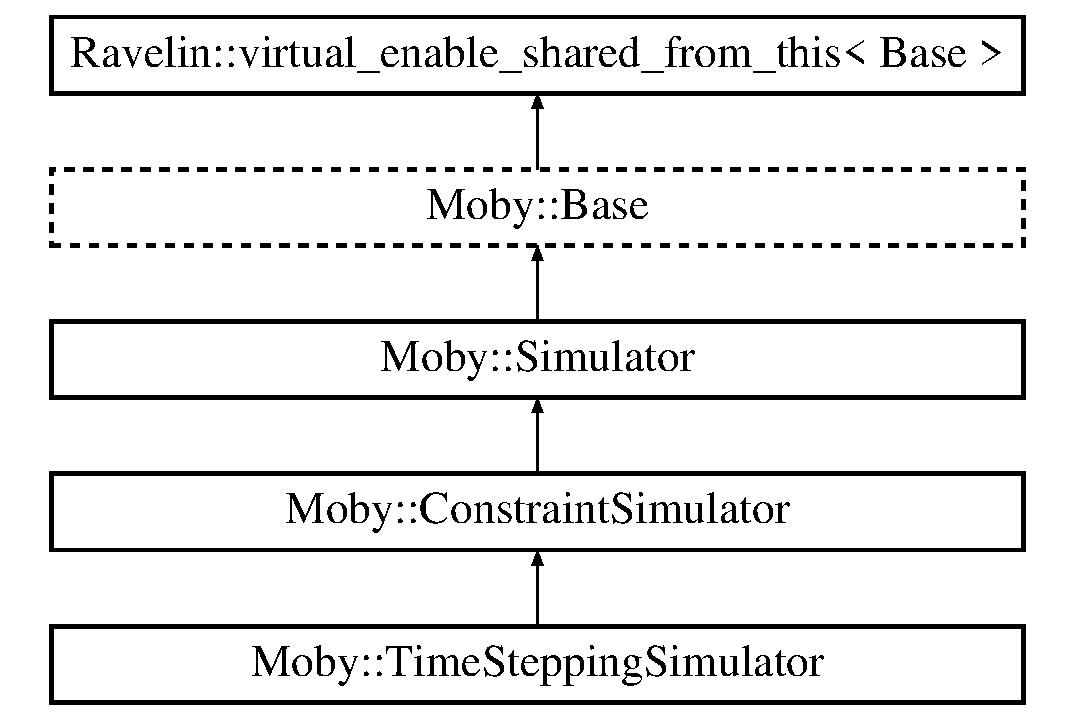
\includegraphics[height=5.000000cm]{classMoby_1_1Simulator}
\end{center}
\end{figure}
\subsection*{Public Member Functions}
\begin{DoxyCompactItemize}
\item 
{\bf Simulator} ()
\begin{DoxyCompactList}\small\item\em Sets up the simulator. \end{DoxyCompactList}\item 
virtual double {\bf step} (double step\-\_\-size)
\begin{DoxyCompactList}\small\item\em Steps the \doxyref{Simulator}{p.}{classMoby_1_1Simulator} forward in time without contact. \end{DoxyCompactList}\item 
{\bf Controlled\-Body\-Ptr} {\bf find\-\_\-dynamic\-\_\-body} (const std\-::string \&name) const 
\begin{DoxyCompactList}\small\item\em Finds the dynamic body in the simulator, if any. \end{DoxyCompactList}\item 
void {\bf add\-\_\-dynamic\-\_\-body} ({\bf Controlled\-Body\-Ptr} body)
\begin{DoxyCompactList}\small\item\em Adds a dynamic body to the simulator. \end{DoxyCompactList}\item 
void {\bf remove\-\_\-dynamic\-\_\-body} ({\bf Controlled\-Body\-Ptr} body)\label{classMoby_1_1Simulator_a60c79b3fdabb58929a54a0781cd6e5f6}

\begin{DoxyCompactList}\small\item\em Removes a dynamic body from the simulator. \end{DoxyCompactList}\item 
void {\bf update\-\_\-visualization} ()\label{classMoby_1_1Simulator_a1e96ca21836ff515d60a6d37645f3643}

\begin{DoxyCompactList}\small\item\em Updates all visualization under the simulator. \end{DoxyCompactList}\item 
virtual void {\bf save\-\_\-to\-\_\-xml} ({\bf X\-M\-L\-Tree\-Ptr} node, std\-::list$<$ boost\-::shared\-\_\-ptr$<$ const {\bf Base} $>$ $>$ \&shared\-\_\-objects) const \label{classMoby_1_1Simulator_a95b0ea5486c10f5c80d088e85f330b12}

\begin{DoxyCompactList}\small\item\em Implements \doxyref{Base\-::save\-\_\-to\-\_\-xml()}{p.}{classMoby_1_1Base_aed64905ca39893d02d1e6c3f03f73aa9} \end{DoxyCompactList}\item 
virtual void {\bf load\-\_\-from\-\_\-xml} (boost\-::shared\-\_\-ptr$<$ const {\bf X\-M\-L\-Tree} $>$ node, std\-::map$<$ std\-::string, {\bf Base\-Ptr} $>$ \&id\-\_\-map)\label{classMoby_1_1Simulator_a8fc61be0cf1e142e0ce9c188eb5b0871}

\begin{DoxyCompactList}\small\item\em Implements \doxyref{Base\-::load\-\_\-from\-\_\-xml()}{p.}{classMoby_1_1Base_a98b861c1d615a748b576aa613f17389f} \end{DoxyCompactList}\item 
const std\-::vector\\*
$<$ {\bf Controlled\-Body\-Ptr} $>$ \& {\bf get\-\_\-dynamic\-\_\-bodies} () const 
\begin{DoxyCompactList}\small\item\em Gets the list of dynamic bodies in the simulator. \end{DoxyCompactList}\item 
void {\bf add\-\_\-transient\-\_\-vdata} (osg\-::\-Node $\ast$vdata)\label{classMoby_1_1Simulator_a648da58d5b65d0543701461203eef60d}

\begin{DoxyCompactList}\small\item\em Adds transient visualization data to the simulator. \end{DoxyCompactList}\item 
osg\-::\-Node $\ast$ {\bf get\-\_\-persistent\-\_\-vdata} () const \label{classMoby_1_1Simulator_ab8e07759b05afd0ec9e9ec3328341750}

\begin{DoxyCompactList}\small\item\em Gets the persistent visualization data. \end{DoxyCompactList}\item 
osg\-::\-Node $\ast$ {\bf get\-\_\-transient\-\_\-vdata} () const \label{classMoby_1_1Simulator_a3929530290f47dcf1983267df5eeae1d}

\begin{DoxyCompactList}\small\item\em Gets the transient (one-\/step) visualization data. \end{DoxyCompactList}\item 
{\footnotesize template$<$class Forward\-Iterator $>$ }\\double {\bf integrate} (double dt, Forward\-Iterator begin, Forward\-Iterator end)
\begin{DoxyCompactList}\small\item\em Integrates both position and velocity of rigid \-\_\-bodies. \end{DoxyCompactList}\end{DoxyCompactItemize}
\subsection*{Public Attributes}
\begin{DoxyCompactItemize}
\item 
double {\bf current\-\_\-time}\label{classMoby_1_1Simulator_a7e49aeda306a8deb91620d1360da30d0}

\begin{DoxyCompactList}\small\item\em The current simulation time. \end{DoxyCompactList}\item 
boost\-::shared\-\_\-ptr$<$ {\bf Dissipation} $>$ {\bf dissipator}\label{classMoby_1_1Simulator_a9769329c255b3054510d869bb1010e81}

\begin{DoxyCompactList}\small\item\em The dissipation mechanism for larger time steps. \end{DoxyCompactList}\item 
void($\ast$ {\bf post\-\_\-step\-\_\-callback\-\_\-fn} )({\bf Simulator} $\ast$s)\label{classMoby_1_1Simulator_a029ab42bc5008ebdda6a74a39466d99b}

\begin{DoxyCompactList}\small\item\em Callback function after a step is completed. \end{DoxyCompactList}\item 
double {\bf dynamics\-\_\-time}\label{classMoby_1_1Simulator_a6d8231190cbe5637d906cc9a8fdf8a54}

\begin{DoxyCompactList}\small\item\em User time spent by dynamics on the last step. \end{DoxyCompactList}\item 
std\-::vector$<$ {\bf Joint\-Ptr} $>$ {\bf implicit\-\_\-joints}\label{classMoby_1_1Simulator_a4327b0b1595b57aeee505d26e986e7af}

\begin{DoxyCompactList}\small\item\em Set of implicit joints maintained in the simulation (does not include implicit joints belonging to \doxyref{R\-C\-Articulated\-Body}{p.}{classMoby_1_1RCArticulatedBody} objects) \end{DoxyCompactList}\end{DoxyCompactItemize}
\subsection*{Protected Member Functions}
\begin{DoxyCompactItemize}
\item 
void {\bf apply\-\_\-impulse} (boost\-::shared\-\_\-ptr$<$ Ravelin\-::\-Dynamic\-Bodyd $>$ db, const Ravelin\-::\-Shared\-Vector\-Nd \&gj)
\begin{DoxyCompactList}\small\item\em Applies a generalized impulse to a dynamic body. \end{DoxyCompactList}\item 
void {\bfseries solve} (const std\-::vector$<$ boost\-::shared\-\_\-ptr$<$ Ravelin\-::\-Dynamic\-Bodyd $>$ $>$ \&island, const std\-::vector$<$ {\bf Joint\-Ptr} $>$ \&island\-\_\-joints, const Ravelin\-::\-Vector\-Nd \&v, const Ravelin\-::\-Vector\-Nd \&f, double dt, Ravelin\-::\-Vector\-Nd \&a, Ravelin\-::\-Vector\-Nd \&lambda) const \label{classMoby_1_1Simulator_a2de1e6596ca7dfc4347b71a7e00ea2fa}

\item 
virtual double {\bfseries check\-\_\-pairwise\-\_\-constraint\-\_\-violations} (double t)\label{classMoby_1_1Simulator_a06649f5f5c3c61fe5bcf9ab97f1b5eee}

\item 
void {\bf find\-\_\-islands} (std\-::vector$<$ std\-::vector$<$ boost\-::shared\-\_\-ptr$<$ Ravelin\-::\-Dynamic\-Bodyd $>$ $>$ $>$ \&islands)\label{classMoby_1_1Simulator_a3f620c8470c2d9452fe6cdc2d0fad78c}

\begin{DoxyCompactList}\small\item\em Finds islands. \end{DoxyCompactList}\item 
unsigned {\bf num\-\_\-generalized\-\_\-coordinates} (const std\-::vector$<$ boost\-::shared\-\_\-ptr$<$ Ravelin\-::\-Dynamic\-Bodyd $>$ $>$ \&island) const \label{classMoby_1_1Simulator_a9a621586cf272fd510a31233ccb3f6ad}

\begin{DoxyCompactList}\small\item\em Gets the number of generalized coordinates in an island. \end{DoxyCompactList}\item 
void {\bf calc\-\_\-fwd\-\_\-dyn} (double dt)\label{classMoby_1_1Simulator_af7c88560f08ca4e9ea567193be931753}

\begin{DoxyCompactList}\small\item\em Calculates forward dynamics for bodies (does not consider unilateral constraints) \end{DoxyCompactList}\item 
void {\bf precalc\-\_\-fwd\-\_\-dyn} ()\label{classMoby_1_1Simulator_a29e3aab680df24c9d153ff7410a1e55a}

\begin{DoxyCompactList}\small\item\em Prepares to calculate forward dynamics for bodies. \end{DoxyCompactList}\item 
{\footnotesize template$<$class Forward\-Iterator $>$ }\\double {\bf integrate} (double step\-\_\-size, Forward\-Iterator begin, Forward\-Iterator end)
\begin{DoxyCompactList}\small\item\em Integrates both position and velocity of rigid \-\_\-bodies. \end{DoxyCompactList}\item 
double {\bf integrate} (double step\-\_\-size)\label{classMoby_1_1Simulator_afe697eeba0574c0767b810c0b417d597}

\begin{DoxyCompactList}\small\item\em Integrates all dynamic bodies. \end{DoxyCompactList}\end{DoxyCompactItemize}
\subsection*{Protected Attributes}
\begin{DoxyCompactItemize}
\item 
osg\-::\-Group $\ast$ {\bfseries \-\_\-persistent\-\_\-vdata}\label{classMoby_1_1Simulator_a0864456d7d22c9bf4727943f004dfa27}

\item 
osg\-::\-Group $\ast$ {\bfseries \-\_\-transient\-\_\-vdata}\label{classMoby_1_1Simulator_aae6b8603ff01832381c7884fb36a8453}

\item 
std\-::vector$<$ {\bf Controlled\-Body\-Ptr} $>$ {\bf \-\_\-bodies}\label{classMoby_1_1Simulator_a93a02b23e0579e76bf8edaa46c0b7f4d}

\begin{DoxyCompactList}\small\item\em The set of bodies in the simulation. \end{DoxyCompactList}\item 
Ravelin\-::\-Vector\-Nd {\bf \-\_\-current\-\_\-dx}\label{classMoby_1_1Simulator_aef259604415abf4d42972ebb203ec109}

\begin{DoxyCompactList}\small\item\em The derivative at the current time. \end{DoxyCompactList}\end{DoxyCompactItemize}
\subsection*{Friends}
\begin{DoxyCompactItemize}
\item 
class {\bfseries Constraint\-Stabilization}\label{classMoby_1_1Simulator_a320e2b5d0cb83071af150f47d50ca127}

\item 
class {\bfseries Impact\-Constraint\-Handler}\label{classMoby_1_1Simulator_a4406c4b5d545224c9183c13d57bca137}

\item 
class {\bfseries Rigid\-Body}\label{classMoby_1_1Simulator_abb8b03bec6b0a8e0834c8358c93039d2}

\item 
class {\bfseries R\-C\-Articulated\-Body}\label{classMoby_1_1Simulator_af04ff9fbc4b43045d831b0922dfad60c}

\end{DoxyCompactItemize}
\subsection*{Additional Inherited Members}


\subsection{Detailed Description}
\doxyref{Simulator}{p.}{classMoby_1_1Simulator} for both unarticulated and articulated rigid bodies without contact. 

Class used for performing dynamics simulation of rigid bodies without contact. Rigid body simulation of articulated bodies is supported using both maximal and reduced coordinate approaches. 

\subsection{Constructor \& Destructor Documentation}
\index{Moby\-::\-Simulator@{Moby\-::\-Simulator}!Simulator@{Simulator}}
\index{Simulator@{Simulator}!Moby::Simulator@{Moby\-::\-Simulator}}
\subsubsection[{Simulator}]{\setlength{\rightskip}{0pt plus 5cm}Simulator\-::\-Simulator (
\begin{DoxyParamCaption}
{}
\end{DoxyParamCaption}
)}\label{classMoby_1_1Simulator_a031573bfcfe2e0f5c9539bcc1c7fc5d9}


Sets up the simulator. 

The simulator properties are set as follows\-: 
\begin{DoxyItemize}
\item simulator time = 0 
\item no integrator 
\end{DoxyItemize}

\subsection{Member Function Documentation}
\index{Moby\-::\-Simulator@{Moby\-::\-Simulator}!add\-\_\-dynamic\-\_\-body@{add\-\_\-dynamic\-\_\-body}}
\index{add\-\_\-dynamic\-\_\-body@{add\-\_\-dynamic\-\_\-body}!Moby::Simulator@{Moby\-::\-Simulator}}
\subsubsection[{add\-\_\-dynamic\-\_\-body}]{\setlength{\rightskip}{0pt plus 5cm}void Simulator\-::add\-\_\-dynamic\-\_\-body (
\begin{DoxyParamCaption}
\item[{{\bf Controlled\-Body\-Ptr}}]{body}
\end{DoxyParamCaption}
)}\label{classMoby_1_1Simulator_ab707346c15456aa36c22d2ae617d583c}


Adds a dynamic body to the simulator. 

\begin{DoxyPrecond}{Precondition}
list of bodies is sorted 
\end{DoxyPrecond}


References Moby\-::\-Visualizable\-::get\-\_\-visualization\-\_\-data().

\index{Moby\-::\-Simulator@{Moby\-::\-Simulator}!apply\-\_\-impulse@{apply\-\_\-impulse}}
\index{apply\-\_\-impulse@{apply\-\_\-impulse}!Moby::Simulator@{Moby\-::\-Simulator}}
\subsubsection[{apply\-\_\-impulse}]{\setlength{\rightskip}{0pt plus 5cm}void Simulator\-::apply\-\_\-impulse (
\begin{DoxyParamCaption}
\item[{boost\-::shared\-\_\-ptr$<$ Ravelin\-::\-Dynamic\-Bodyd $>$}]{db, }
\item[{const Ravelin\-::\-Shared\-Vector\-Nd \&}]{gj}
\end{DoxyParamCaption}
)\hspace{0.3cm}{\ttfamily [protected]}}\label{classMoby_1_1Simulator_a156421c99a5d58eba4bebc6e01594e0c}


Applies a generalized impulse to a dynamic body. 

This function takes implicit constraints into account. \index{Moby\-::\-Simulator@{Moby\-::\-Simulator}!find\-\_\-dynamic\-\_\-body@{find\-\_\-dynamic\-\_\-body}}
\index{find\-\_\-dynamic\-\_\-body@{find\-\_\-dynamic\-\_\-body}!Moby::Simulator@{Moby\-::\-Simulator}}
\subsubsection[{find\-\_\-dynamic\-\_\-body}]{\setlength{\rightskip}{0pt plus 5cm}{\bf Controlled\-Body\-Ptr} Simulator\-::find\-\_\-dynamic\-\_\-body (
\begin{DoxyParamCaption}
\item[{const std\-::string \&}]{name}
\end{DoxyParamCaption}
) const}\label{classMoby_1_1Simulator_abff4d195d3bbb0916ca665446722bdcd}


Finds the dynamic body in the simulator, if any. 

Searches unarticulated bodies, articulated bodies, and links of articulated bodies. \index{Moby\-::\-Simulator@{Moby\-::\-Simulator}!get\-\_\-dynamic\-\_\-bodies@{get\-\_\-dynamic\-\_\-bodies}}
\index{get\-\_\-dynamic\-\_\-bodies@{get\-\_\-dynamic\-\_\-bodies}!Moby::Simulator@{Moby\-::\-Simulator}}
\subsubsection[{get\-\_\-dynamic\-\_\-bodies}]{\setlength{\rightskip}{0pt plus 5cm}const std\-::vector$<${\bf Controlled\-Body\-Ptr}$>$\& Moby\-::\-Simulator\-::get\-\_\-dynamic\-\_\-bodies (
\begin{DoxyParamCaption}
{}
\end{DoxyParamCaption}
) const\hspace{0.3cm}{\ttfamily [inline]}}\label{classMoby_1_1Simulator_a64ecdb2a56b7f76ea91b632f746cdd65}


Gets the list of dynamic bodies in the simulator. 

\begin{DoxyNote}{Note}
if a dynamic body is articulated, only the articulated body is returned, not the links 
\end{DoxyNote}


References \-\_\-bodies.

\index{Moby\-::\-Simulator@{Moby\-::\-Simulator}!integrate@{integrate}}
\index{integrate@{integrate}!Moby::Simulator@{Moby\-::\-Simulator}}
\subsubsection[{integrate}]{\setlength{\rightskip}{0pt plus 5cm}template$<$class Forward\-Iterator $>$ double Moby\-::\-Simulator\-::integrate (
\begin{DoxyParamCaption}
\item[{double}]{dt, }
\item[{Forward\-Iterator}]{begin, }
\item[{Forward\-Iterator}]{end}
\end{DoxyParamCaption}
)}\label{classMoby_1_1Simulator_aeecbb6e84e86c3a7537da15b99d676d7}


Integrates both position and velocity of rigid \-\_\-bodies. 

\begin{DoxyReturn}{Returns}
the size of step taken 
\end{DoxyReturn}
\index{Moby\-::\-Simulator@{Moby\-::\-Simulator}!integrate@{integrate}}
\index{integrate@{integrate}!Moby::Simulator@{Moby\-::\-Simulator}}
\subsubsection[{integrate}]{\setlength{\rightskip}{0pt plus 5cm}template$<$class Forward\-Iterator $>$ double Moby\-::\-Simulator\-::integrate (
\begin{DoxyParamCaption}
\item[{double}]{dt, }
\item[{Forward\-Iterator}]{begin, }
\item[{Forward\-Iterator}]{end}
\end{DoxyParamCaption}
)\hspace{0.3cm}{\ttfamily [protected]}}\label{classMoby_1_1Simulator_a3b3009399c48c49cc71a462cde8c9ca7}


Integrates both position and velocity of rigid \-\_\-bodies. 

\begin{DoxyReturn}{Returns}
the size of step taken 
\end{DoxyReturn}
\index{Moby\-::\-Simulator@{Moby\-::\-Simulator}!step@{step}}
\index{step@{step}!Moby::Simulator@{Moby\-::\-Simulator}}
\subsubsection[{step}]{\setlength{\rightskip}{0pt plus 5cm}double Simulator\-::step (
\begin{DoxyParamCaption}
\item[{double}]{step\-\_\-size}
\end{DoxyParamCaption}
)\hspace{0.3cm}{\ttfamily [virtual]}}\label{classMoby_1_1Simulator_ae22438cc4ed4d1066feda2a2ef0ec0c7}


Steps the \doxyref{Simulator}{p.}{classMoby_1_1Simulator} forward in time without contact. 

This pseudocode was inspired from [Baraff 1997] and [Mirtich 1996]. 
\begin{DoxyParams}{Parameters}
{\em step\-\_\-size} & the step size \\
\hline
\end{DoxyParams}
\begin{DoxyReturn}{Returns}
step\-\_\-size 
\end{DoxyReturn}


Reimplemented in {\bf Moby\-::\-Time\-Stepping\-Simulator} \doxyref{}{p.}{classMoby_1_1TimeSteppingSimulator_a6103f28ca2b879c2edb590ec21a19916}.



The documentation for this class was generated from the following files\-:\begin{DoxyCompactItemize}
\item 
/home/drum/\-Moby/include/\-Moby/Simulator.\-h\item 
/home/drum/\-Moby/include/\-Moby/Simulator.\-inl\item 
/home/drum/\-Moby/src/Simulator.\-cpp\end{DoxyCompactItemize}

\section{Moby\-:\-:Singular\-Exception Class Reference}
\label{classMoby_1_1SingularException}\index{Moby\-::\-Singular\-Exception@{Moby\-::\-Singular\-Exception}}


Exception thrown when trying to invert/solve with a non-\/invertible matrix.  




{\ttfamily \#include $<$Singular\-Exception.\-h$>$}

Inheritance diagram for Moby\-:\-:Singular\-Exception\-:\begin{figure}[H]
\begin{center}
\leavevmode
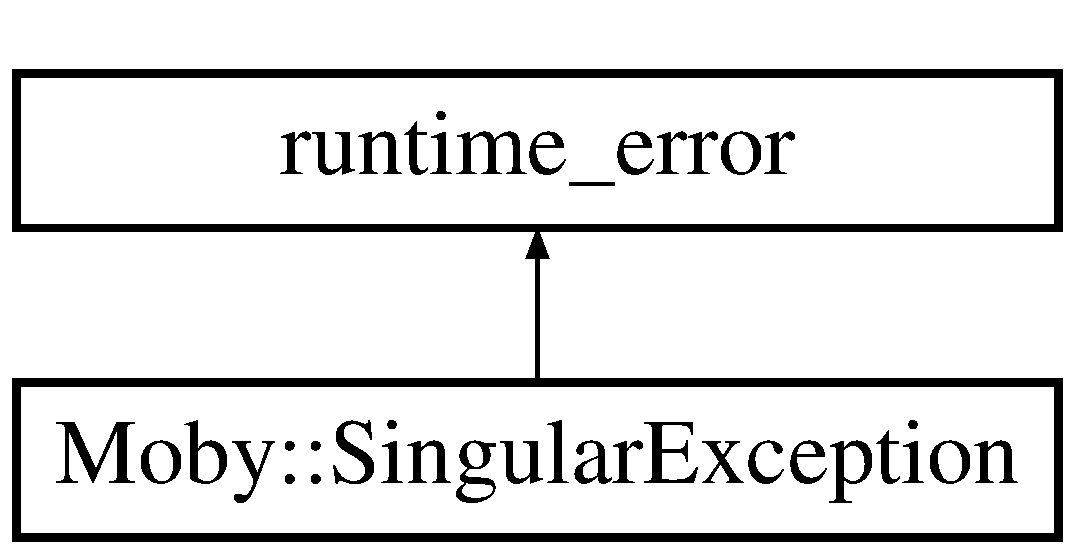
\includegraphics[height=2.000000cm]{classMoby_1_1SingularException}
\end{center}
\end{figure}


\subsection{Detailed Description}
Exception thrown when trying to invert/solve with a non-\/invertible matrix. 

The documentation for this class was generated from the following file\-:\begin{DoxyCompactItemize}
\item 
/home/drum/\-Moby/include/\-Moby/Singular\-Exception.\-h\end{DoxyCompactItemize}

\section{Moby\-:\-:Sparse\-Jacobian Class Reference}
\label{classMoby_1_1SparseJacobian}\index{Moby\-::\-Sparse\-Jacobian@{Moby\-::\-Sparse\-Jacobian}}


A Sparse Jacobian representation along with multiplication routines.  




{\ttfamily \#include $<$Sparse\-Jacobian.\-h$>$}

\subsection*{Public Member Functions}
\begin{DoxyCompactItemize}
\item 
Ravelin\-::\-Vector\-Nd \& {\bfseries mult} (const Ravelin\-::\-Vector\-Nd \&x, Ravelin\-::\-Vector\-Nd \&result) const \label{classMoby_1_1SparseJacobian_a2b1aa47ef0bbeec1929893fabf123bae}

\item 
Ravelin\-::\-Matrix\-Nd \& {\bfseries mult} (const Ravelin\-::\-Matrix\-Nd \&x, Ravelin\-::\-Matrix\-Nd \&result) const \label{classMoby_1_1SparseJacobian_a7e635a806c0446adea1c239fa4242339}

\item 
Ravelin\-::\-Matrix\-Nd \& {\bf transpose\-\_\-mult} (const Ravelin\-::\-Matrix\-Nd \&x, Ravelin\-::\-Matrix\-Nd \&result) const \label{classMoby_1_1SparseJacobian_a9c3ae8255c2125855fe0af74a5e4703d}

\begin{DoxyCompactList}\small\item\em Multiplies the transpose of this sparse Jacobian by a matrix. \end{DoxyCompactList}\item 
Ravelin\-::\-Matrix\-Nd \& {\bfseries mult} (const std\-::vector$<$ {\bf Matrix\-Block} $>$ \&M, unsigned result\-\_\-cols, Ravelin\-::\-Matrix\-Nd \&result) const \label{classMoby_1_1SparseJacobian_ad8fcddbb89a88fef95521b08eff2d650}

\item 
Ravelin\-::\-Matrix\-Nd \& {\bfseries mult} (const std\-::vector$<$ Ravelin\-::\-Matrix\-Nd $>$ \&M, Ravelin\-::\-Matrix\-Nd \&result) const \label{classMoby_1_1SparseJacobian_aa4c84db851ed6e9f2156f680a35dc616}

\item 
Ravelin\-::\-Matrix\-Nd \& {\bf mult\-\_\-transpose} (const {\bf Sparse\-Jacobian} \&M, Ravelin\-::\-Matrix\-Nd \&result) const \label{classMoby_1_1SparseJacobian_af8e6586d8a2ae78ae8970c00e710e84b}

\begin{DoxyCompactList}\small\item\em Multiples this sparse Jacobian by the transpose of another sparse Jacobian. \end{DoxyCompactList}\item 
Ravelin\-::\-Matrix\-Nd \& {\bf to\-\_\-dense} (Ravelin\-::\-Matrix\-Nd \&M) const \label{classMoby_1_1SparseJacobian_a14a24234cbdffea0932d87429a8b3894}

\begin{DoxyCompactList}\small\item\em Converts a sparse Jacobian to a dense matrix (for debugging purposes) \end{DoxyCompactList}\end{DoxyCompactItemize}
\subsection*{Public Attributes}
\begin{DoxyCompactItemize}
\item 
std\-::vector$<$ {\bf Matrix\-Block} $>$ {\bfseries blocks}\label{classMoby_1_1SparseJacobian_aa936e2f4139757a34b44276c3b42f03c}

\item 
unsigned {\bfseries rows}\label{classMoby_1_1SparseJacobian_a920752c96655a2bbfd8869f62665c2b9}

\item 
unsigned {\bfseries cols}\label{classMoby_1_1SparseJacobian_aa1a371cfee664e89cdbf2226714ed3a9}

\end{DoxyCompactItemize}


\subsection{Detailed Description}
A Sparse Jacobian representation along with multiplication routines. 

The documentation for this class was generated from the following files\-:\begin{DoxyCompactItemize}
\item 
/home/drum/\-Moby/include/\-Moby/Sparse\-Jacobian.\-h\item 
/home/drum/\-Moby/src/Sparse\-Jacobian.\-cpp\end{DoxyCompactItemize}

\section{Moby\-:\-:Sphere\-Primitive Class Reference}
\label{classMoby_1_1SpherePrimitive}\index{Moby\-::\-Sphere\-Primitive@{Moby\-::\-Sphere\-Primitive}}


Represents a sphere primitive for inertia properties, collision detection, and visualization.  




{\ttfamily \#include $<$Sphere\-Primitive.\-h$>$}

Inheritance diagram for Moby\-:\-:Sphere\-Primitive\-:\begin{figure}[H]
\begin{center}
\leavevmode
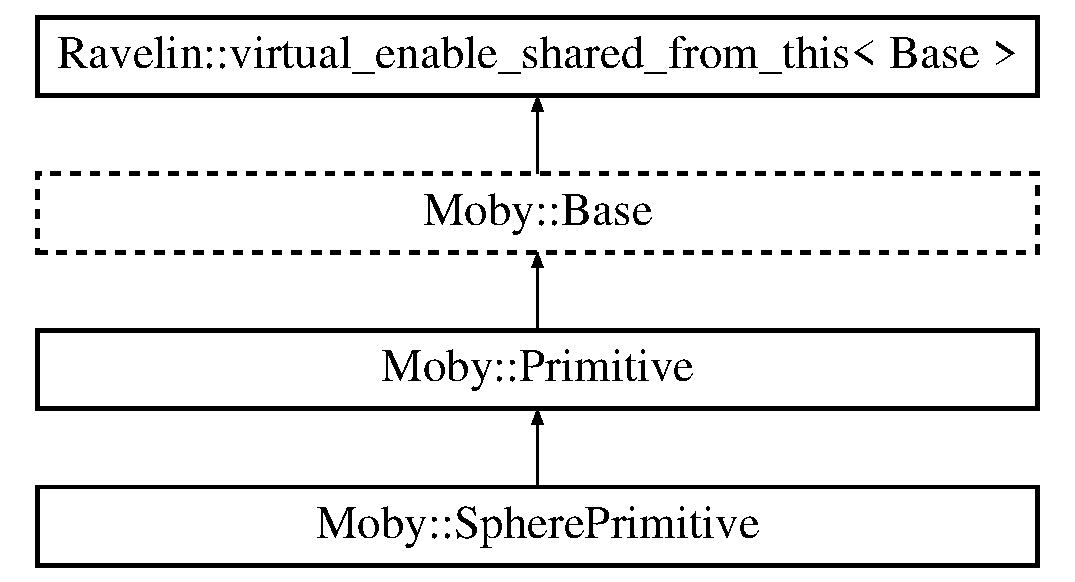
\includegraphics[height=4.000000cm]{classMoby_1_1SpherePrimitive}
\end{center}
\end{figure}
\subsection*{Public Member Functions}
\begin{DoxyCompactItemize}
\item 
{\bf Sphere\-Primitive} ()\label{classMoby_1_1SpherePrimitive_abadd5fec1e03a4e474d7852241b39ed6}

\begin{DoxyCompactList}\small\item\em Creates a sphere with radius 1.\-0 and 100 points. \end{DoxyCompactList}\item 
{\bf Sphere\-Primitive} (double radius)\label{classMoby_1_1SpherePrimitive_a4f26c8a931d27c2eb757000cf43d2eaa}

\begin{DoxyCompactList}\small\item\em Creates a sphere with the specified radius and 100 points. \end{DoxyCompactList}\item 
{\bfseries Sphere\-Primitive} (const Ravelin\-::\-Pose3d \&T)\label{classMoby_1_1SpherePrimitive_a145ad56339b489416f96a900efb16134}

\item 
{\bf Sphere\-Primitive} (double radius, unsigned n)\label{classMoby_1_1SpherePrimitive_a15685e469910c6eeda53c7b1d5cfa907}

\begin{DoxyCompactList}\small\item\em Creates a sphere with the specified radius and number of points. \end{DoxyCompactList}\item 
{\bfseries Sphere\-Primitive} (double radius, const Ravelin\-::\-Pose3d \&T)\label{classMoby_1_1SpherePrimitive_ae57b45e60f11d3ebb006ca5c521c2bb1}

\item 
{\bfseries Sphere\-Primitive} (double radius, unsigned n, const Ravelin\-::\-Pose3d \&T)\label{classMoby_1_1SpherePrimitive_aefe4bcbc7b67726a0b504f4cd442dd90}

\item 
void {\bf set\-\_\-radius} (double radius)\label{classMoby_1_1SpherePrimitive_a7f9757b79fa7bdcb524a2a82fb5886c5}

\begin{DoxyCompactList}\small\item\em Sets the radius for this sphere (forces redetermination of the mesh) \end{DoxyCompactList}\item 
void {\bf set\-\_\-num\-\_\-points} (unsigned n)
\begin{DoxyCompactList}\small\item\em Sets the number of points used in this sphere. \end{DoxyCompactList}\item 
virtual bool {\bf is\-\_\-convex} () const \label{classMoby_1_1SpherePrimitive_a905cde16a1dc04fa37eafc4322b9f7e4}

\begin{DoxyCompactList}\small\item\em Determines whether this primitive is convex. \end{DoxyCompactList}\item 
virtual void {\bf load\-\_\-from\-\_\-xml} (boost\-::shared\-\_\-ptr$<$ const {\bf X\-M\-L\-Tree} $>$ node, std\-::map$<$ std\-::string, {\bf Base\-Ptr} $>$ \&id\-\_\-map)\label{classMoby_1_1SpherePrimitive_abf18dff5adc902467124296cc2972e20}

\begin{DoxyCompactList}\small\item\em Implements \doxyref{Base\-::load\-\_\-from\-\_\-xml()}{p.}{classMoby_1_1Base_a98b861c1d615a748b576aa613f17389f} for serialization. \end{DoxyCompactList}\item 
virtual void {\bf save\-\_\-to\-\_\-xml} ({\bf X\-M\-L\-Tree\-Ptr} node, std\-::list$<$ boost\-::shared\-\_\-ptr$<$ const {\bf Base} $>$ $>$ \&shared\-\_\-objects) const \label{classMoby_1_1SpherePrimitive_a153f43c1030cb7a64f40b316870aac8f}

\begin{DoxyCompactList}\small\item\em Implements \doxyref{Base\-::save\-\_\-to\-\_\-xml()}{p.}{classMoby_1_1Base_aed64905ca39893d02d1e6c3f03f73aa9} for serialization. \end{DoxyCompactList}\item 
virtual void {\bf set\-\_\-pose} (const Ravelin\-::\-Pose3d \&T)\label{classMoby_1_1SpherePrimitive_af317b7dec2cf8dc47eb88f247c45edc2}

\begin{DoxyCompactList}\small\item\em Transforms the primitive. \end{DoxyCompactList}\item 
virtual void {\bf get\-\_\-vertices} (boost\-::shared\-\_\-ptr$<$ const Ravelin\-::\-Pose3d $>$ P, std\-::vector$<$ {\bf Point3d} $>$ \&vertices) const \label{classMoby_1_1SpherePrimitive_a5d19a009a35bf70fe6532a1d286c913a}

\begin{DoxyCompactList}\small\item\em Gets vertices for the primitive. \end{DoxyCompactList}\item 
virtual {\bf B\-V\-Ptr} {\bf get\-\_\-\-B\-V\-H\-\_\-root} ({\bf Collision\-Geometry\-Ptr} geom)\label{classMoby_1_1SpherePrimitive_a87005978b72c0d2f0a3e948d7075afcd}

\begin{DoxyCompactList}\small\item\em Gets the root bounding volume. \end{DoxyCompactList}\item 
virtual double {\bf calc\-\_\-dist\-\_\-and\-\_\-normal} (const {\bf Point3d} \&point, std\-::vector$<$ Ravelin\-::\-Vector3d $>$ \&normals) const \label{classMoby_1_1SpherePrimitive_a2e275d795b285f84b4461257c288342b}

\begin{DoxyCompactList}\small\item\em Finds the signed distance betwen the sphere and a point. \end{DoxyCompactList}\item 
virtual double {\bf calc\-\_\-signed\-\_\-dist} (boost\-::shared\-\_\-ptr$<$ const {\bf Primitive} $>$ p, {\bf Point3d} \&pthis, {\bf Point3d} \&pp) const \label{classMoby_1_1SpherePrimitive_a14afe3ee7eb8bcafe8e9f846a42916b1}

\begin{DoxyCompactList}\small\item\em Computes the signed distance between this and another primitive. \end{DoxyCompactList}\item 
virtual boost\-::shared\-\_\-ptr\\*
$<$ const {\bf Indexed\-Tri\-Array} $>$ {\bf get\-\_\-mesh} (boost\-::shared\-\_\-ptr$<$ const Ravelin\-::\-Pose3d $>$ P)\label{classMoby_1_1SpherePrimitive_aaa9cef7360a44370f5c918efb9ee6f31}

\begin{DoxyCompactList}\small\item\em Gets the mesh, computing it if necessary. \end{DoxyCompactList}\item 
virtual osg\-::\-Node $\ast$ {\bf create\-\_\-visualization} ()\label{classMoby_1_1SpherePrimitive_a9330f200ea8638d08dc05d5f28708fc9}

\begin{DoxyCompactList}\small\item\em Creates the visualization for this primitive. \end{DoxyCompactList}\item 
double {\bfseries calc\-\_\-signed\-\_\-dist} (boost\-::shared\-\_\-ptr$<$ const {\bf Sphere\-Primitive} $>$ s, {\bf Point3d} \&pthis, {\bf Point3d} \&psph) const \label{classMoby_1_1SpherePrimitive_ad56bc76e87e9c7d8403e07ac29134b1c}

\item 
virtual {\bf Point3d} {\bf get\-\_\-supporting\-\_\-point} (const Ravelin\-::\-Vector3d \&d) const \label{classMoby_1_1SpherePrimitive_ae58cf0df84bb5fc03a55d5b3a59d7063}

\begin{DoxyCompactList}\small\item\em Gets the supporting point. \end{DoxyCompactList}\item 
virtual double {\bf calc\-\_\-signed\-\_\-dist} (const {\bf Point3d} \&p) const \label{classMoby_1_1SpherePrimitive_a901a441541f895930ae10d63dbae3d43}

\begin{DoxyCompactList}\small\item\em Computes the signed distance of the given point from this primitive. \end{DoxyCompactList}\item 
virtual double {\bfseries get\-\_\-bounding\-\_\-radius} () const \label{classMoby_1_1SpherePrimitive_ae665b9dfc69a185127300d04bf73336b}

\item 
double {\bf get\-\_\-radius} () const \label{classMoby_1_1SpherePrimitive_add766e3bbd0bb23fb0b7c626bf5a222d}

\begin{DoxyCompactList}\small\item\em Gets the radius for this sphere. \end{DoxyCompactList}\item 
unsigned {\bf get\-\_\-num\-\_\-points} () const \label{classMoby_1_1SpherePrimitive_a0df0f3b3f536deb9fe8f3ea2ee250eff}

\begin{DoxyCompactList}\small\item\em Gets the number of points used to create the sphere for visualization / collision checking. \end{DoxyCompactList}\end{DoxyCompactItemize}
\subsection*{Additional Inherited Members}


\subsection{Detailed Description}
Represents a sphere primitive for inertia properties, collision detection, and visualization. 

\subsection{Member Function Documentation}
\index{Moby\-::\-Sphere\-Primitive@{Moby\-::\-Sphere\-Primitive}!set\-\_\-num\-\_\-points@{set\-\_\-num\-\_\-points}}
\index{set\-\_\-num\-\_\-points@{set\-\_\-num\-\_\-points}!Moby::SpherePrimitive@{Moby\-::\-Sphere\-Primitive}}
\subsubsection[{set\-\_\-num\-\_\-points}]{\setlength{\rightskip}{0pt plus 5cm}void Sphere\-Primitive\-::set\-\_\-num\-\_\-points (
\begin{DoxyParamCaption}
\item[{unsigned}]{n}
\end{DoxyParamCaption}
)}\label{classMoby_1_1SpherePrimitive_ae27120638706eec3c0501e7b50f75364}


Sets the number of points used in this sphere. 


\begin{DoxyParams}{Parameters}
{\em n} & the number of points \\
\hline
\end{DoxyParams}
\begin{DoxyNote}{Note}
forces redetermination of the mesh 
\end{DoxyNote}


Referenced by load\-\_\-from\-\_\-xml().



The documentation for this class was generated from the following files\-:\begin{DoxyCompactItemize}
\item 
/home/drum/\-Moby/include/\-Moby/Sphere\-Primitive.\-h\item 
/home/drum/\-Moby/src/Sphere\-Primitive.\-cpp\end{DoxyCompactItemize}

\section{Moby\-:\-:Spherical\-Joint Class Reference}
\label{classMoby_1_1SphericalJoint}\index{Moby\-::\-Spherical\-Joint@{Moby\-::\-Spherical\-Joint}}


Defines an actuated spherical joint.  




{\ttfamily \#include $<$Spherical\-Joint.\-h$>$}

Inheritance diagram for Moby\-:\-:Spherical\-Joint\-:\begin{figure}[H]
\begin{center}
\leavevmode
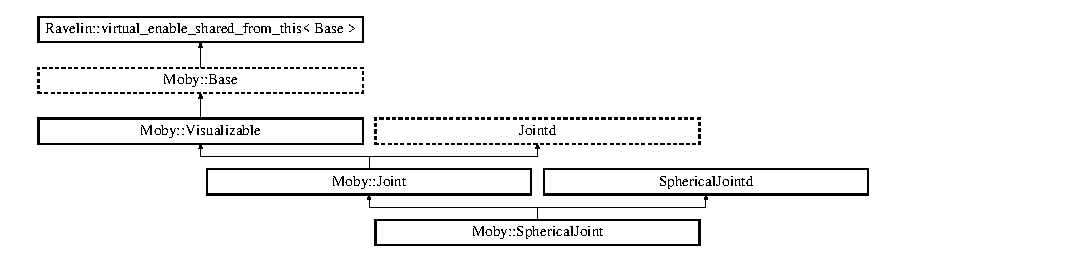
\includegraphics[height=3.070176cm]{classMoby_1_1SphericalJoint}
\end{center}
\end{figure}
\subsection*{Public Member Functions}
\begin{DoxyCompactItemize}
\item 
{\bf Spherical\-Joint} ()
\begin{DoxyCompactList}\small\item\em Initializes the joint. \end{DoxyCompactList}\item 
{\bf Spherical\-Joint} (boost\-::weak\-\_\-ptr$<$ {\bf Rigid\-Body} $>$ inboard, boost\-::weak\-\_\-ptr$<$ {\bf Rigid\-Body} $>$ outboard)
\begin{DoxyCompactList}\small\item\em Initializes the joint with the specified inboard and outboard links. \end{DoxyCompactList}\item 
virtual unsigned {\bfseries num\-\_\-dof} () const \label{classMoby_1_1SphericalJoint_a1350bb54591b748916f848b4081321bb}

\item 
virtual bool {\bfseries is\-\_\-singular\-\_\-config} () const \label{classMoby_1_1SphericalJoint_ab7618c745baf1630589e7fa4b4499fa0}

\item 
virtual void {\bfseries evaluate\-\_\-constraints} (double C[$\,$])\label{classMoby_1_1SphericalJoint_a2d6833566a42976af79d9f55baaa9dad}

\item 
virtual const std\-::vector\\*
$<$ Ravelin\-::\-S\-Velocityd $>$ \& {\bfseries get\-\_\-spatial\-\_\-axes\-\_\-dot} ()\label{classMoby_1_1SphericalJoint_a28e1587ea53e7f11be68e6e52b9fa2f2}

\item 
virtual void {\bfseries determine\-\_\-q} (Ravelin\-::\-Vector\-Nd \&q)\label{classMoby_1_1SphericalJoint_a65072c101fdb9b769aecb4e3184dfc78}

\item 
virtual boost\-::shared\-\_\-ptr\\*
$<$ const Ravelin\-::\-Pose3d $>$ {\bfseries get\-\_\-induced\-\_\-pose} ()\label{classMoby_1_1SphericalJoint_abf9f7c9a1aafc3847f91fefa5ef78795}

\item 
virtual void {\bf load\-\_\-from\-\_\-xml} (boost\-::shared\-\_\-ptr$<$ const {\bf X\-M\-L\-Tree} $>$ node, std\-::map$<$ std\-::string, {\bf Base\-Ptr} $>$ \&id\-\_\-map)\label{classMoby_1_1SphericalJoint_a34675294343bd4326dd20d404476fcd6}

\begin{DoxyCompactList}\small\item\em Implements \doxyref{Base\-::load\-\_\-from\-\_\-xml()}{p.}{classMoby_1_1Base_a98b861c1d615a748b576aa613f17389f} \end{DoxyCompactList}\item 
virtual void {\bf save\-\_\-to\-\_\-xml} ({\bf X\-M\-L\-Tree\-Ptr} node, std\-::list$<$ boost\-::shared\-\_\-ptr$<$ const {\bf Base} $>$ $>$ \&shared\-\_\-objects) const \label{classMoby_1_1SphericalJoint_a620cb80de5502c45583e7c74ebfa7ba1}

\begin{DoxyCompactList}\small\item\em Implements \doxyref{Base\-::save\-\_\-to\-\_\-xml()}{p.}{classMoby_1_1Base_aed64905ca39893d02d1e6c3f03f73aa9} \end{DoxyCompactList}\end{DoxyCompactItemize}
\subsection*{Additional Inherited Members}


\subsection{Detailed Description}
Defines an actuated spherical joint. 

\subsection{Constructor \& Destructor Documentation}
\index{Moby\-::\-Spherical\-Joint@{Moby\-::\-Spherical\-Joint}!Spherical\-Joint@{Spherical\-Joint}}
\index{Spherical\-Joint@{Spherical\-Joint}!Moby::SphericalJoint@{Moby\-::\-Spherical\-Joint}}
\subsubsection[{Spherical\-Joint}]{\setlength{\rightskip}{0pt plus 5cm}Spherical\-Joint\-::\-Spherical\-Joint (
\begin{DoxyParamCaption}
{}
\end{DoxyParamCaption}
)}\label{classMoby_1_1SphericalJoint_ab8f7df4760955b6b67b561d077a21d10}


Initializes the joint. 

The axes of rotation are each set to [0 0 0]. The inboard and outboard links are set to N\-U\-L\-L. 

References Moby\-::\-Joint\-::init\-\_\-data().

\index{Moby\-::\-Spherical\-Joint@{Moby\-::\-Spherical\-Joint}!Spherical\-Joint@{Spherical\-Joint}}
\index{Spherical\-Joint@{Spherical\-Joint}!Moby::SphericalJoint@{Moby\-::\-Spherical\-Joint}}
\subsubsection[{Spherical\-Joint}]{\setlength{\rightskip}{0pt plus 5cm}Spherical\-Joint\-::\-Spherical\-Joint (
\begin{DoxyParamCaption}
\item[{boost\-::weak\-\_\-ptr$<$ {\bf Rigid\-Body} $>$}]{inboard, }
\item[{boost\-::weak\-\_\-ptr$<$ {\bf Rigid\-Body} $>$}]{outboard}
\end{DoxyParamCaption}
)}\label{classMoby_1_1SphericalJoint_a6344f9a3403a89e845175a5ec249e8f7}


Initializes the joint with the specified inboard and outboard links. 

The axis of rotation is set to [0 0 0]. 

The documentation for this class was generated from the following files\-:\begin{DoxyCompactItemize}
\item 
/home/drum/\-Moby/include/\-Moby/Spherical\-Joint.\-h\item 
/home/drum/\-Moby/src/Spherical\-Joint.\-cpp\end{DoxyCompactItemize}

\section{Moby\-:\-:S\-S\-L Class Reference}
\label{classMoby_1_1SSL}\index{Moby\-::\-S\-S\-L@{Moby\-::\-S\-S\-L}}


A sphere-\/swept line (\doxyref{S\-S\-L}{p.}{classMoby_1_1SSL}) that optionally allows building an \doxyref{S\-S\-L}{p.}{classMoby_1_1SSL} tree.  




{\ttfamily \#include $<$S\-S\-L.\-h$>$}

Inheritance diagram for Moby\-:\-:S\-S\-L\-:\begin{figure}[H]
\begin{center}
\leavevmode
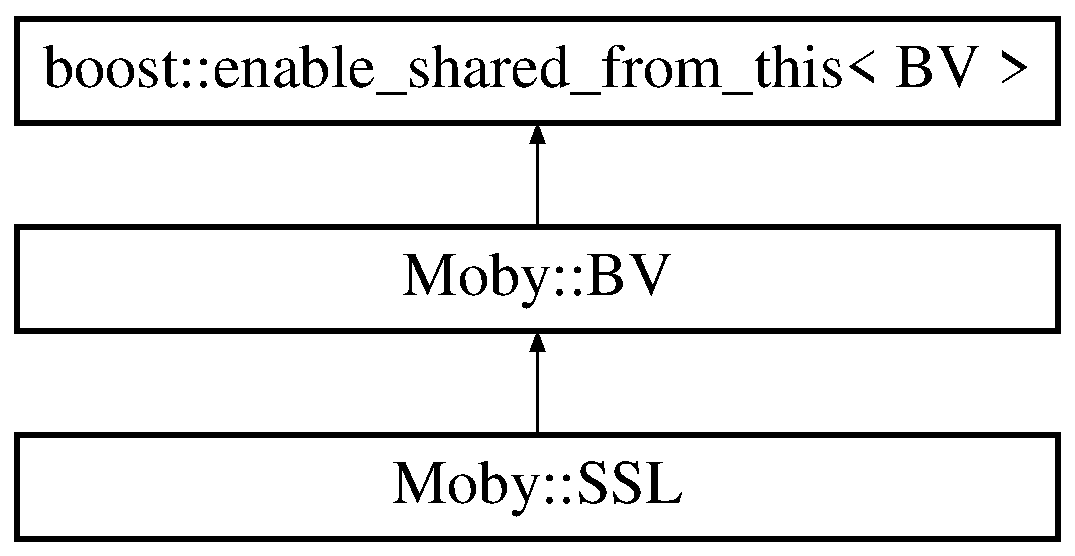
\includegraphics[height=3.000000cm]{classMoby_1_1SSL}
\end{center}
\end{figure}
\subsection*{Public Member Functions}
\begin{DoxyCompactItemize}
\item 
{\bf S\-S\-L} ()\label{classMoby_1_1SSL_ab5fad6b6b913f8373162231040829fa8}

\begin{DoxyCompactList}\small\item\em Initializes an empty \doxyref{S\-S\-L}{p.}{classMoby_1_1SSL}. \end{DoxyCompactList}\item 
{\bfseries S\-S\-L} (const {\bf S\-S\-L} \&obb)\label{classMoby_1_1SSL_aff636b617cb61b04d4932ddf8b1277bf}

\item 
{\bf S\-S\-L} (const {\bf Point3d} \&{\bf p1}, const {\bf Point3d} \&{\bf p2}, double {\bf radius})\label{classMoby_1_1SSL_a52c88d87c5b2cd60560a314c868608db}

\begin{DoxyCompactList}\small\item\em Initializes a \doxyref{S\-S\-L}{p.}{classMoby_1_1SSL} from the given values. \end{DoxyCompactList}\item 
{\bfseries S\-S\-L} (const {\bf S\-S\-L} \&s, const Ravelin\-::\-Vector3d \&v)\label{classMoby_1_1SSL_acaf7d1c0e7cccae8d2967664d4ac471b}

\item 
{\bf S\-S\-L} \& {\bf operator=} (const {\bf S\-S\-L} \&s)\label{classMoby_1_1SSL_aaf79f8a9e5c1ecbaeb1277b0fb119aba}

\begin{DoxyCompactList}\small\item\em Copies one \doxyref{S\-S\-L}{p.}{classMoby_1_1SSL} to another. \end{DoxyCompactList}\item 
virtual void {\bf transform} (const Ravelin\-::\-Transform3d \&T, {\bf B\-V} $\ast$result) const \label{classMoby_1_1SSL_a8b353299fb254e39dca28deda8078d84}

\begin{DoxyCompactList}\small\item\em Transforms the \doxyref{S\-S\-L}{p.}{classMoby_1_1SSL} using the given transform. \end{DoxyCompactList}\item 
virtual {\bf B\-V\-Ptr} {\bf calc\-\_\-swept\-\_\-\-B\-V} ({\bf Collision\-Geometry\-Ptr} g, const Ravelin\-::\-S\-Velocityd \&v) const \label{classMoby_1_1SSL_a6984388248b9437ce29433de1a264234}

\begin{DoxyCompactList}\small\item\em Calculates the velocity-\/expanded bounding volume. \end{DoxyCompactList}\item 
virtual bool {\bf intersects} (const {\bf Line\-Seg3} \&seg, double \&tmin, double tmax, {\bf Point3d} \&q) const \label{classMoby_1_1SSL_ab205ccce0f836469625a75aea794bb8e}

\begin{DoxyCompactList}\small\item\em Determines whether a line segment intersects the bounding volume. \end{DoxyCompactList}\item 
virtual bool {\bf outside} (const {\bf Point3d} \&point, double tol=N\-E\-A\-R\-\_\-\-Z\-E\-R\-O) const \label{classMoby_1_1SSL_aac14e017684280b0ebf45929b01ddf2b}

\begin{DoxyCompactList}\small\item\em Determines whether a point is outside the bounding volume. \end{DoxyCompactList}\item 
boost\-::shared\-\_\-ptr$<$ {\bf S\-S\-L} $>$ {\bfseries get\-\_\-this} ()\label{classMoby_1_1SSL_a8f1486ea726e7b4cf7b6df70c8b5f02d}

\item 
boost\-::shared\-\_\-ptr$<$ const {\bf S\-S\-L} $>$ {\bfseries get\-\_\-this} () const \label{classMoby_1_1SSL_a7602d505a815004794329c404823a09d}

\item 
virtual std\-::ostream \& {\bf to\-\_\-vrml} (std\-::ostream \&out, const Ravelin\-::\-Pose3d \&T) const \label{classMoby_1_1SSL_af43430a716fbbb826d74147575f62db9}

\begin{DoxyCompactList}\small\item\em Outputs the \doxyref{S\-S\-L}{p.}{classMoby_1_1SSL} to V\-R\-M\-L (not yet implemented) \end{DoxyCompactList}\item 
unsigned {\bf calc\-\_\-size} () const \label{classMoby_1_1SSL_a440ff5c757b3ea94f0e071e258219932}

\begin{DoxyCompactList}\small\item\em Calculates the size (number of elements in) a \doxyref{S\-S\-L}{p.}{classMoby_1_1SSL} tree. \end{DoxyCompactList}\item 
virtual boost\-::shared\-\_\-ptr\\*
$<$ const Ravelin\-::\-Pose3d $>$ {\bf get\-\_\-relative\-\_\-pose} () const \label{classMoby_1_1SSL_a4e1e627916b22674b1662094735fcc1c}

\begin{DoxyCompactList}\small\item\em Gets the associated pose for this bounding volume. \end{DoxyCompactList}\item 
virtual {\bf Point3d} {\bf get\-\_\-lower\-\_\-bounds} () const \label{classMoby_1_1SSL_adf1bbe2d6cf4261665d0a2b5f3fcf92e}

\begin{DoxyCompactList}\small\item\em Gets the lower bounds of the \doxyref{S\-S\-L}{p.}{classMoby_1_1SSL}. \end{DoxyCompactList}\item 
virtual {\bf Point3d} {\bf get\-\_\-upper\-\_\-bounds} () const \label{classMoby_1_1SSL_a92fb9325b3b776970ab5a904debc8ee2}

\begin{DoxyCompactList}\small\item\em Gets the upper bounds of the \doxyref{S\-S\-L}{p.}{classMoby_1_1SSL}. \end{DoxyCompactList}\item 
virtual double {\bf calc\-\_\-volume} () const \label{classMoby_1_1SSL_ac1ba452b2d95c028575c7958d16d81a7}

\begin{DoxyCompactList}\small\item\em Calculates (approximate?) volume of the \doxyref{S\-S\-L}{p.}{classMoby_1_1SSL}. \end{DoxyCompactList}\end{DoxyCompactItemize}
\subsection*{Static Public Member Functions}
\begin{DoxyCompactItemize}
\item 
static double {\bf calc\-\_\-dist} (const {\bf S\-S\-L} \&o, const {\bf Point3d} \&p)\label{classMoby_1_1SSL_a166bbd791f7258ca87a4fb5862bc1f45}

\begin{DoxyCompactList}\small\item\em Calculates the distance of the sphere-\/swept line from a point. \end{DoxyCompactList}\item 
static double {\bf calc\-\_\-dist} (const {\bf S\-S\-L} \&a, const {\bf S\-S\-L} \&b, {\bf Point3d} \&cpa, {\bf Point3d} \&cpb)\label{classMoby_1_1SSL_a95a5b76ff550fd7bfbcf685028a1453b}

\begin{DoxyCompactList}\small\item\em Calculates the distance between two sphere-\/swept lines and also calculates closest points. \end{DoxyCompactList}\item 
static double {\bfseries calc\-\_\-dist} (const {\bf S\-S\-L} \&a, const {\bf S\-S\-L} \&b, const Ravelin\-::\-Transform3d \&a\-Tb, {\bf Point3d} \&cpa, {\bf Point3d} \&cpb)\label{classMoby_1_1SSL_a0232d1635147bd1633dd15560b815fe8}

\item 
static bool {\bf intersects} (const {\bf S\-S\-L} \&a, const {\bf S\-S\-L} \&b)\label{classMoby_1_1SSL_a6289697931b62da21faef5d36a78a5be}

\begin{DoxyCompactList}\small\item\em Determines whether two S\-S\-Ls intersect. \end{DoxyCompactList}\item 
static bool {\bfseries intersects} (const {\bf S\-S\-L} \&a, const {\bf S\-S\-L} \&b, const Ravelin\-::\-Transform3d \&a\-Tb)\label{classMoby_1_1SSL_a1e50b42599045b88909b0280aef6e22f}

\item 
static bool {\bf intersects} (const {\bf S\-S\-L} \&a, const {\bf Line\-Seg3} \&seg, double \&tmin, double tmax, {\bf Point3d} \&q)\label{classMoby_1_1SSL_a60d5a569d63eb7664c2915600b1858ce}

\begin{DoxyCompactList}\small\item\em Determines whether (and when) a line segment intersects with the \doxyref{S\-S\-L}{p.}{classMoby_1_1SSL}. \end{DoxyCompactList}\item 
static bool {\bf outside} (const {\bf S\-S\-L} \&a, const {\bf Point3d} \&point, double tol=N\-E\-A\-R\-\_\-\-Z\-E\-R\-O)\label{classMoby_1_1SSL_af483c88fea5031a8664f7e6172524d43}

\begin{DoxyCompactList}\small\item\em Determines whether a point is outside the \doxyref{S\-S\-L}{p.}{classMoby_1_1SSL}. \end{DoxyCompactList}\end{DoxyCompactItemize}
\subsection*{Public Attributes}
\begin{DoxyCompactItemize}
\item 
{\bf Point3d} {\bf p1}\label{classMoby_1_1SSL_a2693320556687c9826eb74c0f36b09bf}

\begin{DoxyCompactList}\small\item\em The first point of the line segment. \end{DoxyCompactList}\item 
{\bf Point3d} {\bf p2}\label{classMoby_1_1SSL_a606a8aa6ae6d8452ee74db400af65b87}

\begin{DoxyCompactList}\small\item\em The second point of the line segment. \end{DoxyCompactList}\item 
double {\bf radius}\label{classMoby_1_1SSL_ad8db6aece89c6c37ff9835027e75d4ee}

\begin{DoxyCompactList}\small\item\em Radius of the spherical addition. \end{DoxyCompactList}\end{DoxyCompactItemize}


\subsection{Detailed Description}
A sphere-\/swept line (\doxyref{S\-S\-L}{p.}{classMoby_1_1SSL}) that optionally allows building an \doxyref{S\-S\-L}{p.}{classMoby_1_1SSL} tree. 

The documentation for this class was generated from the following files\-:\begin{DoxyCompactItemize}
\item 
/home/drum/\-Moby/include/\-Moby/S\-S\-L.\-h\item 
/home/drum/\-Moby/src/S\-S\-L.\-cpp\end{DoxyCompactItemize}

\section{Moby\-:\-:S\-S\-R Class Reference}
\label{classMoby_1_1SSR}\index{Moby\-::\-S\-S\-R@{Moby\-::\-S\-S\-R}}


A sphere-\/swept rectangle (\doxyref{S\-S\-R}{p.}{classMoby_1_1SSR}) that optionally allows building an \doxyref{S\-S\-R}{p.}{classMoby_1_1SSR} tree.  




{\ttfamily \#include $<$S\-S\-R.\-h$>$}

Inheritance diagram for Moby\-:\-:S\-S\-R\-:\begin{figure}[H]
\begin{center}
\leavevmode
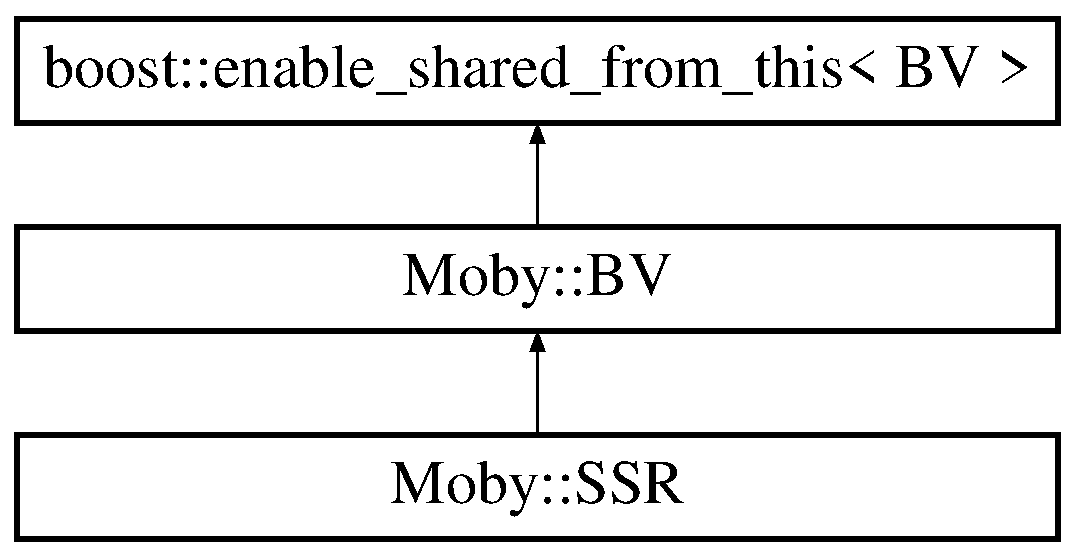
\includegraphics[height=3.000000cm]{classMoby_1_1SSR}
\end{center}
\end{figure}
\subsection*{Public Member Functions}
\begin{DoxyCompactItemize}
\item 
{\bf S\-S\-R} ()\label{classMoby_1_1SSR_a8b7a80a3ec1bc78e64b0b069eb19c737}

\begin{DoxyCompactList}\small\item\em Initializes an empty \doxyref{S\-S\-R}{p.}{classMoby_1_1SSR}. \end{DoxyCompactList}\item 
{\bfseries S\-S\-R} (const {\bf S\-S\-R} \&obb)\label{classMoby_1_1SSR_ad8a85ac82ef78ab0fb03befae3a2cd89}

\item 
{\bfseries S\-S\-R} (const {\bf Point3d} \&{\bf center}, const Ravelin\-::\-Matrix3d \&{\bf R}, const Ravelin\-::\-Vector2d \&{\bf l}, double {\bf radius})\label{classMoby_1_1SSR_a368ab6f63ce991291872779ae14e9bba}

\item 
{\bfseries S\-S\-R} (const {\bf S\-S\-R} \&s, const Ravelin\-::\-Vector3d \&v)\label{classMoby_1_1SSR_a69797b20abd3b0abae48b929a0abaeb7}

\item 
{\bf S\-S\-R} \& {\bf operator=} (const {\bf S\-S\-R} \&s)\label{classMoby_1_1SSR_acd4e477698da7453c32e97f60fc89fe0}

\begin{DoxyCompactList}\small\item\em Copies one \doxyref{S\-S\-R}{p.}{classMoby_1_1SSR} to another. \end{DoxyCompactList}\item 
virtual {\bf B\-V\-Ptr} {\bf calc\-\_\-swept\-\_\-\-B\-V} ({\bf Collision\-Geometry\-Ptr} g, const Ravelin\-::\-S\-Velocityd \&v) const \label{classMoby_1_1SSR_a455c8f91015dc88fd82e401d29cc3b04}

\begin{DoxyCompactList}\small\item\em Calculates the velocity-\/expanded bounding volume. \end{DoxyCompactList}\item 
virtual bool {\bf intersects} (const {\bf Line\-Seg3} \&seg, double \&tmin, double tmax, {\bf Point3d} \&q) const \label{classMoby_1_1SSR_a5a17e7fa50ffdb425049b75be85734fa}

\begin{DoxyCompactList}\small\item\em Determines whether a line segment intersects the bounding volume. \end{DoxyCompactList}\item 
virtual bool {\bf outside} (const {\bf Point3d} \&point, double tol=N\-E\-A\-R\-\_\-\-Z\-E\-R\-O) const \label{classMoby_1_1SSR_acd2ea5e0313f6a2c3ca6f8f087f7b904}

\begin{DoxyCompactList}\small\item\em Determines whether a point is outside the bounding volume. \end{DoxyCompactList}\item 
boost\-::shared\-\_\-ptr$<$ {\bf S\-S\-R} $>$ {\bfseries get\-\_\-this} ()\label{classMoby_1_1SSR_ad22e44ac5bfe323b74826c134690b5ac}

\item 
boost\-::shared\-\_\-ptr$<$ const {\bf S\-S\-R} $>$ {\bfseries get\-\_\-this} () const \label{classMoby_1_1SSR_a70a14b94eec7efb7300d09746e41d1f2}

\item 
virtual std\-::ostream \& {\bf to\-\_\-vrml} (std\-::ostream \&out, const Ravelin\-::\-Pose3d \&T) const \label{classMoby_1_1SSR_a1534431dfb9e4da2ba73a15f693a8107}

\begin{DoxyCompactList}\small\item\em Outputs the \doxyref{S\-S\-R}{p.}{classMoby_1_1SSR} to V\-R\-M\-L (not yet implemented) \end{DoxyCompactList}\item 
unsigned {\bf calc\-\_\-size} () const \label{classMoby_1_1SSR_a6fbf22c3b8bb9a03ecf369e060c1f246}

\begin{DoxyCompactList}\small\item\em Calculates the size (number of elements in) a \doxyref{S\-S\-R}{p.}{classMoby_1_1SSR} tree. \end{DoxyCompactList}\item 
virtual boost\-::shared\-\_\-ptr\\*
$<$ const Ravelin\-::\-Pose3d $>$ {\bf get\-\_\-relative\-\_\-pose} () const \label{classMoby_1_1SSR_a314f75152b9681be4670284326310f45}

\begin{DoxyCompactList}\small\item\em Gets the associated pose for this bounding volume. \end{DoxyCompactList}\item 
virtual void {\bf transform} (const Ravelin\-::\-Transform3d \&T, {\bf B\-V} $\ast$result) const \label{classMoby_1_1SSR_ab46f39d7948d926c2ebe3dad6da6a340}

\begin{DoxyCompactList}\small\item\em Transforms the \doxyref{S\-S\-R}{p.}{classMoby_1_1SSR} using the given transform. \end{DoxyCompactList}\item 
virtual {\bf Point3d} {\bf get\-\_\-lower\-\_\-bounds} () const \label{classMoby_1_1SSR_a6e74e7d2c6d3141692cfa586d669fbcf}

\begin{DoxyCompactList}\small\item\em Gets the lower bounds of the \doxyref{S\-S\-R}{p.}{classMoby_1_1SSR}. \end{DoxyCompactList}\item 
virtual {\bf Point3d} {\bf get\-\_\-upper\-\_\-bounds} () const \label{classMoby_1_1SSR_a20bbc7a25648c73d0140efe135b0418d}

\begin{DoxyCompactList}\small\item\em Gets the upper bounds of the \doxyref{S\-S\-R}{p.}{classMoby_1_1SSR}. \end{DoxyCompactList}\item 
void {\bf get\-\_\-rect\-\_\-verts} ({\bf Point3d} rect\-\_\-verts[4]) const \label{classMoby_1_1SSR_a78262822eee90c81506f986bb56d2f48}

\begin{DoxyCompactList}\small\item\em Gets the vertices of the rectangle. \end{DoxyCompactList}\item 
{\footnotesize template$<$class Forward\-Iterator $>$ }\\void {\bfseries expand\-\_\-to\-\_\-fit} (Forward\-Iterator begin, Forward\-Iterator end)\label{classMoby_1_1SSR_a855fa235a4504adf5a523408af608c39}

\item 
{\footnotesize template$<$class Forward\-Iterator $>$ }\\{\bf S\-S\-R} (Forward\-Iterator begin, Forward\-Iterator end)
\begin{DoxyCompactList}\small\item\em Computes a \doxyref{S\-S\-R}{p.}{classMoby_1_1SSR} from a set of points. \end{DoxyCompactList}\item 
virtual double {\bf calc\-\_\-volume} () const \label{classMoby_1_1SSR_a37a04d5c42adfcc84454d1d8e8f85fbb}

\begin{DoxyCompactList}\small\item\em Calculates (approximate?) volume of the \doxyref{S\-S\-R}{p.}{classMoby_1_1SSR}. \end{DoxyCompactList}\item 
{\footnotesize template$<$class Forward\-Iterator $>$ }\\{\bf S\-S\-R} (Forward\-Iterator begin, Forward\-Iterator end)
\begin{DoxyCompactList}\small\item\em Computes a \doxyref{S\-S\-R}{p.}{classMoby_1_1SSR} from a set of points. \end{DoxyCompactList}\item 
{\footnotesize template$<$class Forward\-Iterator $>$ }\\void {\bf calc\-\_\-lengths\-\_\-and\-\_\-radius} (Forward\-Iterator begin, Forward\-Iterator end)\label{classMoby_1_1SSR_a3dcd98770b11bd2504d8e76f2c8303e9}

\begin{DoxyCompactList}\small\item\em Calculates the lengths and radius for a \doxyref{S\-S\-R}{p.}{classMoby_1_1SSR}. \end{DoxyCompactList}\item 
{\footnotesize template$<$class Forward\-Iterator $>$ }\\void {\bf align} (Forward\-Iterator begin, Forward\-Iterator end, const Ravelin\-::\-Vector3d \&d1, Ravelin\-::\-Vector3d \&d2)\label{classMoby_1_1SSR_abbae6ed4b2ce9fa3d34d5484d34502db}

\begin{DoxyCompactList}\small\item\em Aligns this \doxyref{S\-S\-R}{p.}{classMoby_1_1SSR} with the minimum area bounding rectangle projected along the first dimension of the \doxyref{S\-S\-R}{p.}{classMoby_1_1SSR}. \end{DoxyCompactList}\end{DoxyCompactItemize}
\subsection*{Static Public Member Functions}
\begin{DoxyCompactItemize}
\item 
static double {\bf calc\-\_\-dist} (const {\bf S\-S\-R} \&a, const {\bf Point3d} \&p)\label{classMoby_1_1SSR_a8d3cb92a9f46fe056a15ee98275d26ab}

\begin{DoxyCompactList}\small\item\em Calculates the distance of the sphere-\/swept rectangle from a point. \end{DoxyCompactList}\item 
static double {\bf calc\-\_\-dist} (const {\bf S\-S\-R} \&a, const {\bf Line\-Seg3} \&s)\label{classMoby_1_1SSR_aed16e801077911e2f625c6608976b827}

\begin{DoxyCompactList}\small\item\em Calculates the distance of the sphere-\/swept rectangle from a line segment. \end{DoxyCompactList}\item 
static double {\bf calc\-\_\-dist} (const {\bf S\-S\-R} \&a, const {\bf S\-S\-R} \&b, {\bf Point3d} \&cpa, {\bf Point3d} \&cpb)\label{classMoby_1_1SSR_a122c7a2340345bb402db2a76e85ef904}

\begin{DoxyCompactList}\small\item\em Calculates the distance between two sphere-\/swept rectangles and also calculates closest points. \end{DoxyCompactList}\item 
static double {\bfseries calc\-\_\-dist} (const {\bf S\-S\-R} \&a, const {\bf S\-S\-R} \&b, const Ravelin\-::\-Transform3d \&a\-Tb, {\bf Point3d} \&cpa, {\bf Point3d} \&cpb)\label{classMoby_1_1SSR_aab5efd4465c3a61141196ba97e49fab2}

\item 
static bool {\bf intersects} (const {\bf S\-S\-R} \&a, const {\bf S\-S\-R} \&b)\label{classMoby_1_1SSR_a6cb93fa494830b7620115bdf50d8ec1c}

\begin{DoxyCompactList}\small\item\em Determines whether two S\-S\-Rs intersect. \end{DoxyCompactList}\item 
static bool {\bfseries intersects} (const {\bf S\-S\-R} \&a, const {\bf S\-S\-R} \&b, const Ravelin\-::\-Transform3d \&T)\label{classMoby_1_1SSR_a85dc6ab72902166f9555685e887ca327}

\item 
static bool {\bf intersects} (const {\bf S\-S\-R} \&a, const {\bf Line\-Seg3} \&seg, double \&tmin, double tmax, {\bf Point3d} \&q)\label{classMoby_1_1SSR_a986cdd5d771558d5ab67d551699fc9b6}

\begin{DoxyCompactList}\small\item\em Determines whether (and when) a line segment intersects with the \doxyref{S\-S\-R}{p.}{classMoby_1_1SSR}. \end{DoxyCompactList}\item 
static bool {\bf outside} (const {\bf S\-S\-R} \&a, const {\bf Point3d} \&point, double tol=N\-E\-A\-R\-\_\-\-Z\-E\-R\-O)\label{classMoby_1_1SSR_a9f6b32da9911b69a2dea09fb5f917a28}

\begin{DoxyCompactList}\small\item\em Determines whether a point is outside the \doxyref{S\-S\-R}{p.}{classMoby_1_1SSR}. \end{DoxyCompactList}\end{DoxyCompactItemize}
\subsection*{Public Attributes}
\begin{DoxyCompactItemize}
\item 
{\bf Point3d} {\bf center}\label{classMoby_1_1SSR_a6a800bdb4056f75e334597fd0d46371e}

\begin{DoxyCompactList}\small\item\em Center of the volume. \end{DoxyCompactList}\item 
Ravelin\-::\-Vector2d {\bf l}\label{classMoby_1_1SSR_ac88d95c6c5bccb8abfc2ee7f553db346}

\begin{DoxyCompactList}\small\item\em Lengths of the rectangle sides. \end{DoxyCompactList}\item 
Ravelin\-::\-Matrix3d {\bf R}\label{classMoby_1_1SSR_a78b018270d95f253135b543927111b29}

\begin{DoxyCompactList}\small\item\em Orientation of this \doxyref{S\-S\-R}{p.}{classMoby_1_1SSR}. \end{DoxyCompactList}\item 
double {\bf radius}\label{classMoby_1_1SSR_aa88f142592fb8d0ec8ee4b1126374d00}

\begin{DoxyCompactList}\small\item\em Radius of the spherical addition. \end{DoxyCompactList}\end{DoxyCompactItemize}


\subsection{Detailed Description}
A sphere-\/swept rectangle (\doxyref{S\-S\-R}{p.}{classMoby_1_1SSR}) that optionally allows building an \doxyref{S\-S\-R}{p.}{classMoby_1_1SSR} tree. 

\begin{DoxyNote}{Note}
the \doxyref{S\-S\-R}{p.}{classMoby_1_1SSR} is generally constructed such that its frame is aligned with that of the underlying rigid body (or collision geometry). Therefore, the center of the \doxyref{S\-S\-R}{p.}{classMoby_1_1SSR} is computed relative to the center-\/of-\/mass of the body (or the center of the geometry). The orientation of the \doxyref{S\-S\-R}{p.}{classMoby_1_1SSR} will always be identical to the orientation of the rigid body (or collision geometry). 
\end{DoxyNote}


\subsection{Constructor \& Destructor Documentation}
\index{Moby\-::\-S\-S\-R@{Moby\-::\-S\-S\-R}!S\-S\-R@{S\-S\-R}}
\index{S\-S\-R@{S\-S\-R}!Moby::SSR@{Moby\-::\-S\-S\-R}}
\subsubsection[{S\-S\-R}]{\setlength{\rightskip}{0pt plus 5cm}template$<$class Forward\-Iterator $>$ Moby\-::\-S\-S\-R\-::\-S\-S\-R (
\begin{DoxyParamCaption}
\item[{Forward\-Iterator}]{begin, }
\item[{Forward\-Iterator}]{end}
\end{DoxyParamCaption}
)}\label{classMoby_1_1SSR_ae7789823238913fb00c9c54230dfbca9}


Computes a \doxyref{S\-S\-R}{p.}{classMoby_1_1SSR} from a set of points. 


\begin{DoxyParams}{Parameters}
{\em begin} & an iterator to type Point3d \\
\hline
{\em end} & an iterator to type Point3d Algorithm taken from [Ericson, 2005] \\
\hline
\end{DoxyParams}
\index{Moby\-::\-S\-S\-R@{Moby\-::\-S\-S\-R}!S\-S\-R@{S\-S\-R}}
\index{S\-S\-R@{S\-S\-R}!Moby::SSR@{Moby\-::\-S\-S\-R}}
\subsubsection[{S\-S\-R}]{\setlength{\rightskip}{0pt plus 5cm}template$<$class Forward\-Iterator $>$ Moby\-::\-S\-S\-R\-::\-S\-S\-R (
\begin{DoxyParamCaption}
\item[{Forward\-Iterator}]{begin, }
\item[{Forward\-Iterator}]{end}
\end{DoxyParamCaption}
)}\label{classMoby_1_1SSR_ae7789823238913fb00c9c54230dfbca9}


Computes a \doxyref{S\-S\-R}{p.}{classMoby_1_1SSR} from a set of points. 


\begin{DoxyParams}{Parameters}
{\em begin} & an iterator to type Point3d \\
\hline
{\em end} & an iterator to type Point3d Algorithm taken from [Ericson, 2005] \\
\hline
\end{DoxyParams}


References Moby\-::\-Indexed\-Tri\-::a, Moby\-::\-Indexed\-Tri\-::b, and Moby\-::\-Indexed\-Tri\-::c.



The documentation for this class was generated from the following files\-:\begin{DoxyCompactItemize}
\item 
/home/drum/\-Moby/include/\-Moby/S\-S\-R.\-h\item 
/home/drum/\-Moby/include/\-Moby/S\-S\-R.\-inl\item 
/home/drum/\-Moby/src/S\-S\-R.\-cpp\end{DoxyCompactItemize}

\section{Moby\-:\-:Stokes\-Drag\-Force Class Reference}
\label{classMoby_1_1StokesDragForce}\index{Moby\-::\-Stokes\-Drag\-Force@{Moby\-::\-Stokes\-Drag\-Force}}
Inheritance diagram for Moby\-:\-:Stokes\-Drag\-Force\-:\begin{figure}[H]
\begin{center}
\leavevmode
\includegraphics[height=4.000000cm]{classMoby_1_1StokesDragForce}
\end{center}
\end{figure}
\subsection*{Public Member Functions}
\begin{DoxyCompactItemize}
\item 
{\bf Stokes\-Drag\-Force} ()\label{classMoby_1_1StokesDragForce_ad6401265759d2712c489447bce4559d2}

\begin{DoxyCompactList}\small\item\em Constructs a default drag coefficient of 0. \end{DoxyCompactList}\item 
{\bf Stokes\-Drag\-Force} (const {\bf Stokes\-Drag\-Force} \&source)\label{classMoby_1_1StokesDragForce_aed6fb4070eb8ad16402a38054ab57fed}

\begin{DoxyCompactList}\small\item\em Copy constructor. \end{DoxyCompactList}\item 
virtual void {\bf add\-\_\-force} (boost\-::shared\-\_\-ptr$<$ Ravelin\-::\-Dynamic\-Bodyd $>$ body)\label{classMoby_1_1StokesDragForce_a53f0d2a8e9752fee491647baec985d4b}

\begin{DoxyCompactList}\small\item\em Adds gravity to a body. \end{DoxyCompactList}\item 
virtual void {\bf load\-\_\-from\-\_\-xml} (boost\-::shared\-\_\-ptr$<$ const {\bf X\-M\-L\-Tree} $>$ node, std\-::map$<$ std\-::string, {\bf Base\-Ptr} $>$ \&id\-\_\-map)\label{classMoby_1_1StokesDragForce_aa89874941cd4860ff97d8ea0cb3af524}

\begin{DoxyCompactList}\small\item\em Implements \doxyref{Base\-::load\-\_\-from\-\_\-xml()}{p.}{classMoby_1_1Base_a98b861c1d615a748b576aa613f17389f} \end{DoxyCompactList}\item 
virtual void {\bf save\-\_\-to\-\_\-xml} ({\bf X\-M\-L\-Tree\-Ptr} node, std\-::list$<$ boost\-::shared\-\_\-ptr$<$ const {\bf Base} $>$ $>$ \&shared\-\_\-objects) const \label{classMoby_1_1StokesDragForce_a0b072b877cff16bee5113d1fecbeccaa}

\begin{DoxyCompactList}\small\item\em Implements \doxyref{Base\-::save\-\_\-to\-\_\-xml()}{p.}{classMoby_1_1Base_aed64905ca39893d02d1e6c3f03f73aa9} \end{DoxyCompactList}\end{DoxyCompactItemize}
\subsection*{Public Attributes}
\begin{DoxyCompactItemize}
\item 
double {\bf b}\label{classMoby_1_1StokesDragForce_a6b2aa6e4930192107f90637a3cb74996}

\begin{DoxyCompactList}\small\item\em The drag coefficient. \end{DoxyCompactList}\item 
double {\bfseries b\-\_\-ang}\label{classMoby_1_1StokesDragForce_ae15577967f0fe1a76c6b15705c36b293}

\end{DoxyCompactItemize}
\subsection*{Additional Inherited Members}


The documentation for this class was generated from the following files\-:\begin{DoxyCompactItemize}
\item 
/home/drum/\-Moby/include/\-Moby/Stokes\-Drag\-Force.\-h\item 
/home/drum/\-Moby/src/Stokes\-Drag\-Force.\-cpp\end{DoxyCompactItemize}

\section{Moby\-:\-:Tessellated\-Polyhedron Class Reference}
\label{classMoby_1_1TessellatedPolyhedron}\index{Moby\-::\-Tessellated\-Polyhedron@{Moby\-::\-Tessellated\-Polyhedron}}


Represents a three-\/dimensional polyhedron.  




{\ttfamily \#include $<$Tessellated\-Polyhedron.\-h$>$}

\subsection*{Public Types}
\begin{DoxyCompactItemize}
\item 
enum {\bfseries Location\-Type} \{ \\*
{\bfseries e\-Inside}, 
{\bfseries e\-Outside}, 
{\bfseries e\-On\-Vertex}, 
{\bfseries e\-On\-Edge}, 
\\*
{\bfseries e\-On\-Face}
 \}
\end{DoxyCompactItemize}
\subsection*{Public Member Functions}
\begin{DoxyCompactItemize}
\item 
{\bf Tessellated\-Polyhedron} (const {\bf Indexed\-Tri\-Array} \&mesh)\label{classMoby_1_1TessellatedPolyhedron_a7ead23f84f059e92089595986b5e28e6}

\begin{DoxyCompactList}\small\item\em Constructs a polyhedron from an indexed triangle array. \end{DoxyCompactList}\item 
{\bfseries Tessellated\-Polyhedron} (const {\bf Tessellated\-Polyhedron} \&p)\label{classMoby_1_1TessellatedPolyhedron_aa0c0d73d6fbc4c5ecad717ddbb0bb1a7}

\item 
void {\bf operator=} (const {\bf Tessellated\-Polyhedron} \&p)\label{classMoby_1_1TessellatedPolyhedron_a0048b8bc7fb6dc592cb51eb816c460a8}

\begin{DoxyCompactList}\small\item\em Copies a polyhedron. \end{DoxyCompactList}\item 
const {\bf Indexed\-Tri\-Array} \& {\bfseries get\-\_\-mesh} () const \label{classMoby_1_1TessellatedPolyhedron_af5c2d899c1dcc7023bff5da90e387d16}

\item 
void {\bf transform} (const Ravelin\-::\-Transform3d \&T)
\begin{DoxyCompactList}\small\item\em Transforms this polyhedron by the given transformation matrix. \end{DoxyCompactList}\item 
const std\-::vector\\*
$<$ Ravelin\-::\-Origin3d $>$ \& {\bfseries get\-\_\-vertices} () const \label{classMoby_1_1TessellatedPolyhedron_afb6e0574db44c6325d3642e255b5eefd}

\item 
const std\-::vector$<$ {\bf Indexed\-Tri} $>$ \& {\bfseries get\-\_\-facets} () const \label{classMoby_1_1TessellatedPolyhedron_acdab14afb1e3ed1a4c84186ce5bd58b6}

\item 
bool {\bf inside} (const Ravelin\-::\-Origin3d \&point, double tol=N\-E\-A\-R\-\_\-\-Z\-E\-R\-O)\label{classMoby_1_1TessellatedPolyhedron_ab30dad674b5734565e47e19277cae8a9}

\begin{DoxyCompactList}\small\item\em Determines whether the specified point is strictly inside this polyhedron. \end{DoxyCompactList}\item 
bool {\bf inside\-\_\-or\-\_\-on} (const Ravelin\-::\-Origin3d \&point, double tol=N\-E\-A\-R\-\_\-\-Z\-E\-R\-O)\label{classMoby_1_1TessellatedPolyhedron_a3e3bd639bbaa7ba4fd2cade2951a95df}

\begin{DoxyCompactList}\small\item\em Determines whether the specified point is in or on this polyhedron. \end{DoxyCompactList}\item 
Location\-Type {\bf location} (const Ravelin\-::\-Origin3d \&point, double tol=N\-E\-A\-R\-\_\-\-Z\-E\-R\-O) const 
\begin{DoxyCompactList}\small\item\em Determines the location of the specified point with respect to this polyhedron. \end{DoxyCompactList}\item 
double {\bf calc\-\_\-volume} () const \label{classMoby_1_1TessellatedPolyhedron_aea105a30886607fef7b795e1818605aa}

\begin{DoxyCompactList}\small\item\em Calculates the volume of this polyhedron. \end{DoxyCompactList}\item 
bool {\bf consistent} () const \label{classMoby_1_1TessellatedPolyhedron_a2b6919cac83be190d5d83cdc9e5d8b97}

\begin{DoxyCompactList}\small\item\em Checks whether this polyhedron is consistent. \end{DoxyCompactList}\item 
bool {\bf degenerate} () const \label{classMoby_1_1TessellatedPolyhedron_a08b57b1e27308ccba41c42870a8b26b4}

\begin{DoxyCompactList}\small\item\em Checks whether this polyhedron is degenerate. \end{DoxyCompactList}\item 
const Ravelin\-::\-Origin3d \& {\bf find\-\_\-extreme\-\_\-vertex} (const Ravelin\-::\-Origin3d \&direction)\label{classMoby_1_1TessellatedPolyhedron_ab58f2c681e870aca8b29f2c64197ef99}

\begin{DoxyCompactList}\small\item\em Does an extremal point query for the \doxyref{Polyhedron}{p.}{classMoby_1_1Polyhedron}; returns a vertex furthest along the given direction. \end{DoxyCompactList}\item 
void {\bf to\-\_\-polyhedron} ({\bf Polyhedron} \&p) const \label{classMoby_1_1TessellatedPolyhedron_a49211a929e0eaeba431e2551d3ec503a}

\begin{DoxyCompactList}\small\item\em Creates a polyhedron from this tessellated polyhedron. \end{DoxyCompactList}\item 
{\footnotesize template$<$class Input\-Iterator1 , class Input\-Iterator2 $>$ }\\{\bf Tessellated\-Polyhedron} (Input\-Iterator1 verts\-\_\-begin, Input\-Iterator1 verts\-\_\-end, Input\-Iterator2 facets\-\_\-begin, Input\-Iterator2 facets\-\_\-end)\label{classMoby_1_1TessellatedPolyhedron_a6cdf73cbcceb70f75068fd65cc2c42bc}

\begin{DoxyCompactList}\small\item\em Constructs a \doxyref{Tessellated\-Polyhedron}{p.}{classMoby_1_1TessellatedPolyhedron} from iterators to a container holding Point3d objects and iterators to a container holding \doxyref{Indexed\-Tri}{p.}{structMoby_1_1IndexedTri} types. \end{DoxyCompactList}\item 
const std\-::list$<$ unsigned $>$ \& {\bf get\-\_\-incident\-\_\-facets} (unsigned i) const \label{classMoby_1_1TessellatedPolyhedron_a339fc3ba0dee67d21e5ef8f83e36f66d}

\begin{DoxyCompactList}\small\item\em Gets the list of facets coincident to the i'th facet. \end{DoxyCompactList}\item 
double {\bf calc\-\_\-signed\-\_\-distance} (const Ravelin\-::\-Origin3d \&point, unsigned \&closest\-\_\-facet)\label{classMoby_1_1TessellatedPolyhedron_a8dd674fa7a73d0d321fa1da9d6429d33}

\begin{DoxyCompactList}\small\item\em Gets the signed distance and closest facet to a point. \end{DoxyCompactList}\item 
double {\bf calc\-\_\-signed\-\_\-distance} (const Ravelin\-::\-Origin3d \&point)\label{classMoby_1_1TessellatedPolyhedron_a95fed822ef3c08f8673e3ff9517cf164}

\begin{DoxyCompactList}\small\item\em Gets the signed distance from a point to the polyhedron. \end{DoxyCompactList}\item 
std\-::pair$<$ Ravelin\-::\-Origin3d, \\*
Ravelin\-::\-Origin3d $>$ {\bf get\-\_\-bounding\-\_\-box\-\_\-corners} () const \label{classMoby_1_1TessellatedPolyhedron_a215084b8331ce5f3de7c2ca051bd0bf6}

\begin{DoxyCompactList}\small\item\em Gets the corners of the axis-\/aligned bounding box of this polyhedron. \end{DoxyCompactList}\item 
bool {\bf is\-\_\-convex} ()\label{classMoby_1_1TessellatedPolyhedron_a13556119b58cb31d86a56485165bdaee}

\begin{DoxyCompactList}\small\item\em Determines whether this polyhedron convex (to w/in floating point tolerance) \end{DoxyCompactList}\item 
double {\bf convexity} ()
\begin{DoxyCompactList}\small\item\em Gets the convexity of this polyhedron. \end{DoxyCompactList}\item 
{\footnotesize template$<$class Input\-Iterator1 , class Input\-Iterator2 $>$ }\\{\bf Tessellated\-Polyhedron} (Input\-Iterator1 verts\-\_\-begin, Input\-Iterator1 verts\-\_\-end, Input\-Iterator2 facets\-\_\-begin, Input\-Iterator2 facets\-\_\-end)\label{classMoby_1_1TessellatedPolyhedron_a6cdf73cbcceb70f75068fd65cc2c42bc}

\begin{DoxyCompactList}\small\item\em Constructs a \doxyref{Tessellated\-Polyhedron}{p.}{classMoby_1_1TessellatedPolyhedron} from iterators to a container holding Point3d objects and iterators to a container holding \doxyref{Indexed\-Tri}{p.}{structMoby_1_1IndexedTri} types. \end{DoxyCompactList}\end{DoxyCompactItemize}
\subsection*{Static Public Member Functions}
\begin{DoxyCompactItemize}
\item 
static {\bf Tessellated\-Polyhedron\-Ptr} {\bf minkowski} ({\bf Tessellated\-Polyhedron} \&p1, boost\-::shared\-\_\-ptr$<$ const Ravelin\-::\-Pose3d $>$ T1, {\bf Tessellated\-Polyhedron} \&p2, boost\-::shared\-\_\-ptr$<$ const Ravelin\-::\-Pose3d $>$ T2, bool reflect\-\_\-p2=true)\label{classMoby_1_1TessellatedPolyhedron_a2aee844dc6e24d29e66501f795a3a586}

\begin{DoxyCompactList}\small\item\em Computes the Minkowski sum of two convex polyhedra. \end{DoxyCompactList}\item 
static void {\bf to\-\_\-vrml} (std\-::ostream \&out, const {\bf Tessellated\-Polyhedron} \&p, Ravelin\-::\-Origin3d diffuse\-\_\-color=Ravelin\-::\-Origin3d(1, 1, 1), bool wireframe=false)\label{classMoby_1_1TessellatedPolyhedron_a0fe69af0073c28ba703813ba5f767315}

\begin{DoxyCompactList}\small\item\em Sends this polyhedron to the specified stream using V\-R\-M\-L. \end{DoxyCompactList}\item 
static {\bf Indexed\-Tri\-Array} {\bf construct\-\_\-intersection} ({\bf Tessellated\-Polyhedron} \&p1, {\bf Tessellated\-Polyhedron} \&p2)
\begin{DoxyCompactList}\small\item\em Intersects two non-\/convex polyhedra. \end{DoxyCompactList}\item 
static {\bf Indexed\-Tri\-Array} {\bf construct\-\_\-union} ({\bf Tessellated\-Polyhedron} \&p1, {\bf Tessellated\-Polyhedron} \&p2)\label{classMoby_1_1TessellatedPolyhedron_a94b90dec84d4f8250f9526a85a9010e8}

\begin{DoxyCompactList}\small\item\em Unions two non-\/convex polyhedra. \end{DoxyCompactList}\item 
static {\bf Indexed\-Tri\-Array} {\bf construct\-\_\-difference} ({\bf Tessellated\-Polyhedron} \&p1, {\bf Tessellated\-Polyhedron} \&p2)\label{classMoby_1_1TessellatedPolyhedron_a206a3cde718fff8404c89a61a17a84c2}

\begin{DoxyCompactList}\small\item\em Constructs the Boolean difference p1 -\/ p2. \end{DoxyCompactList}\end{DoxyCompactItemize}


\subsection{Detailed Description}
Represents a three-\/dimensional polyhedron. 

Though this class is used for representing polyhedron, it is possible to represent arbitrary (i.\-e., non-\/closed) triangle meshes as well. 

\subsection{Member Function Documentation}
\index{Moby\-::\-Tessellated\-Polyhedron@{Moby\-::\-Tessellated\-Polyhedron}!construct\-\_\-intersection@{construct\-\_\-intersection}}
\index{construct\-\_\-intersection@{construct\-\_\-intersection}!Moby::TessellatedPolyhedron@{Moby\-::\-Tessellated\-Polyhedron}}
\subsubsection[{construct\-\_\-intersection}]{\setlength{\rightskip}{0pt plus 5cm}{\bf Indexed\-Tri\-Array} Tessellated\-Polyhedron\-::construct\-\_\-intersection (
\begin{DoxyParamCaption}
\item[{{\bf Tessellated\-Polyhedron} \&}]{p1, }
\item[{{\bf Tessellated\-Polyhedron} \&}]{p2}
\end{DoxyParamCaption}
)\hspace{0.3cm}{\ttfamily [static]}}\label{classMoby_1_1TessellatedPolyhedron_aa7695754e171614f333cc01b7225e111}


Intersects two non-\/convex polyhedra. 

The running time for this algorithm is O(nm), where n and m are the number of triangles of p1 and p2, respectively. A faster algorithm can be obtained if p1 and p2 are both convex, but it is not implemented here. 

References Moby\-::\-Indexed\-Tri\-Array\-::compress\-\_\-vertices(), and consistent().

\index{Moby\-::\-Tessellated\-Polyhedron@{Moby\-::\-Tessellated\-Polyhedron}!convexity@{convexity}}
\index{convexity@{convexity}!Moby::TessellatedPolyhedron@{Moby\-::\-Tessellated\-Polyhedron}}
\subsubsection[{convexity}]{\setlength{\rightskip}{0pt plus 5cm}double Moby\-::\-Tessellated\-Polyhedron\-::convexity (
\begin{DoxyParamCaption}
{}
\end{DoxyParamCaption}
)\hspace{0.3cm}{\ttfamily [inline]}}\label{classMoby_1_1TessellatedPolyhedron_ab21e51eaae09b0338c55840519717ab9}


Gets the convexity of this polyhedron. 

Convexity values less than epsilon (where epsilon is some number near zero) indicate that the polyhedron is convex; greater values indicate that the polyhedron is non-\/convex. 

Referenced by is\-\_\-convex().

\index{Moby\-::\-Tessellated\-Polyhedron@{Moby\-::\-Tessellated\-Polyhedron}!location@{location}}
\index{location@{location}!Moby::TessellatedPolyhedron@{Moby\-::\-Tessellated\-Polyhedron}}
\subsubsection[{location}]{\setlength{\rightskip}{0pt plus 5cm}Tessellated\-Polyhedron\-::\-Location\-Type Tessellated\-Polyhedron\-::location (
\begin{DoxyParamCaption}
\item[{const Ravelin\-::\-Origin3d \&}]{point, }
\item[{double}]{tol = {\ttfamily NEAR\-\_\-ZERO}}
\end{DoxyParamCaption}
) const}\label{classMoby_1_1TessellatedPolyhedron_ad1e2a218d8573d47129c88667de77739}


Determines the location of the specified point with respect to this polyhedron. 

This method handles queries when the polyhedron is not convex or more detail is necessary. Adapted from O'Rourke, p. 247-\/250. Runs in worst-\/case time O(f), where f is the number of facets of the polyhedron. \index{Moby\-::\-Tessellated\-Polyhedron@{Moby\-::\-Tessellated\-Polyhedron}!transform@{transform}}
\index{transform@{transform}!Moby::TessellatedPolyhedron@{Moby\-::\-Tessellated\-Polyhedron}}
\subsubsection[{transform}]{\setlength{\rightskip}{0pt plus 5cm}void Tessellated\-Polyhedron\-::transform (
\begin{DoxyParamCaption}
\item[{const Ravelin\-::\-Transform3d \&}]{T}
\end{DoxyParamCaption}
)}\label{classMoby_1_1TessellatedPolyhedron_af5795156db49a618e12f74886b91be92}


Transforms this polyhedron by the given transformation matrix. 

\begin{DoxyNote}{Note}
none of the vertex or triangle pointers change; rather the data that they point to changes 
\end{DoxyNote}


Referenced by minkowski().



The documentation for this class was generated from the following files\-:\begin{DoxyCompactItemize}
\item 
/home/drum/\-Moby/include/\-Moby/Tessellated\-Polyhedron.\-h\item 
/home/drum/\-Moby/include/\-Moby/Tessellated\-Polyhedron.\-inl\item 
/home/drum/\-Moby/src/Tessellated\-Polyhedron.\-cpp\end{DoxyCompactItemize}

\section{Moby\-:\-:Time\-Stepping\-Simulator Class Reference}
\label{classMoby_1_1TimeSteppingSimulator}\index{Moby\-::\-Time\-Stepping\-Simulator@{Moby\-::\-Time\-Stepping\-Simulator}}


An event-\/driven simulator.  




{\ttfamily \#include $<$Time\-Stepping\-Simulator.\-h$>$}

Inheritance diagram for Moby\-:\-:Time\-Stepping\-Simulator\-:\begin{figure}[H]
\begin{center}
\leavevmode
\includegraphics[height=5.000000cm]{classMoby_1_1TimeSteppingSimulator}
\end{center}
\end{figure}
\subsection*{Public Member Functions}
\begin{DoxyCompactItemize}
\item 
{\bf Time\-Stepping\-Simulator} ()\label{classMoby_1_1TimeSteppingSimulator_a3869d581d50a88702b5834a177ceb08a}

\begin{DoxyCompactList}\small\item\em Default constructor. \end{DoxyCompactList}\item 
virtual void {\bf load\-\_\-from\-\_\-xml} (boost\-::shared\-\_\-ptr$<$ const {\bf X\-M\-L\-Tree} $>$ node, std\-::map$<$ std\-::string, {\bf Base\-Ptr} $>$ \&id\-\_\-map)\label{classMoby_1_1TimeSteppingSimulator_a1b29397680cc9ca652eaf790b77d0191}

\begin{DoxyCompactList}\small\item\em Implements \doxyref{Base\-::load\-\_\-from\-\_\-xml()}{p.}{classMoby_1_1Base_a98b861c1d615a748b576aa613f17389f} \end{DoxyCompactList}\item 
virtual void {\bf save\-\_\-to\-\_\-xml} ({\bf X\-M\-L\-Tree\-Ptr} node, std\-::list$<$ boost\-::shared\-\_\-ptr$<$ const {\bf Base} $>$ $>$ \&shared\-\_\-objects) const \label{classMoby_1_1TimeSteppingSimulator_a9fbe88f409947ebdec530bf0d221182c}

\begin{DoxyCompactList}\small\item\em Implements \doxyref{Base\-::save\-\_\-to\-\_\-xml()}{p.}{classMoby_1_1Base_aed64905ca39893d02d1e6c3f03f73aa9} \end{DoxyCompactList}\item 
virtual double {\bf step} (double dt)\label{classMoby_1_1TimeSteppingSimulator_a6103f28ca2b879c2edb590ec21a19916}

\begin{DoxyCompactList}\small\item\em Steps the simulator forward by the given step size. \end{DoxyCompactList}\item 
boost\-::shared\-\_\-ptr\\*
$<$ {\bf Contact\-Parameters} $>$ {\bfseries get\-\_\-contact\-\_\-parameters} ({\bf Collision\-Geometry\-Ptr} geom1, {\bf Collision\-Geometry\-Ptr} geom2) const \label{classMoby_1_1TimeSteppingSimulator_a45aeafaf5b009c82e9a8be6b48be8d49}

\item 
boost\-::shared\-\_\-ptr\\*
$<$ {\bf Time\-Stepping\-Simulator} $>$ {\bf get\-\_\-this} ()\label{classMoby_1_1TimeSteppingSimulator_a3381f9eb3ba491db30f5ec879ac64461}

\begin{DoxyCompactList}\small\item\em Gets the shared pointer for this. \end{DoxyCompactList}\end{DoxyCompactItemize}
\subsection*{Public Attributes}
\begin{DoxyCompactItemize}
\item 
double {\bfseries min\-\_\-step\-\_\-size}\label{classMoby_1_1TimeSteppingSimulator_a7aa770057f4173c95b911b1ff62c9f44}

\item 
std\-::set$<$ Ravelin\-::sorted\-\_\-pair\\*
$<$ {\bf Collision\-Geometry\-Ptr} $>$ $>$ {\bf unchecked\-\_\-pairs}\label{classMoby_1_1TimeSteppingSimulator_afe14d868006c6e17f5225fca5446b698}

\begin{DoxyCompactList}\small\item\em Determines whether two geometries are not checked. \end{DoxyCompactList}\item 
std\-::vector$<$ std\-::pair\\*
$<$ {\bf Controlled\-Body\-Ptr}, \\*
Ravelin\-::\-Vector\-Nd $>$ $>$ {\bf \-\_\-x0}\label{classMoby_1_1TimeSteppingSimulator_a3143eb8cdc343a4c03fcaafa838c33ee}

\begin{DoxyCompactList}\small\item\em Vectors set and passed to collision detection. \end{DoxyCompactList}\item 
std\-::vector$<$ std\-::pair\\*
$<$ {\bf Controlled\-Body\-Ptr}, \\*
Ravelin\-::\-Vector\-Nd $>$ $>$ {\bfseries \-\_\-x1}\label{classMoby_1_1TimeSteppingSimulator_aefd27d4e5adc40c725ff7b9c37993318}

\end{DoxyCompactItemize}
\subsection*{Protected Member Functions}
\begin{DoxyCompactItemize}
\item 
bool {\bf constraints\-\_\-met} (const std\-::vector$<$ {\bf Pairwise\-Dist\-Info} $>$ \&current\-\_\-pairwise\-\_\-distances)\label{classMoby_1_1TimeSteppingSimulator_a28526e4aa5e5dda8768d42968752fcce}

\begin{DoxyCompactList}\small\item\em Checks to see whether all constraints are met. \end{DoxyCompactList}\item 
std\-::set$<$ Ravelin\-::sorted\-\_\-pair\\*
$<$ {\bf Collision\-Geometry\-Ptr} $>$ $>$ {\bf get\-\_\-current\-\_\-contact\-\_\-geoms} () const \label{classMoby_1_1TimeSteppingSimulator_a6841e6a4a5865ed8d740c02ef5aebcdc}

\begin{DoxyCompactList}\small\item\em Gets the current set of contact geometries. \end{DoxyCompactList}\item 
double {\bf do\-\_\-mini\-\_\-step} (double dt)\label{classMoby_1_1TimeSteppingSimulator_a6c2059048eaf1f77c60cc611e3f2c5e7}

\begin{DoxyCompactList}\small\item\em Does a full integration cycle (but not necessarily a full step) \end{DoxyCompactList}\item 
void {\bf step\-\_\-si\-\_\-\-Euler} (double dt)
\begin{DoxyCompactList}\small\item\em Does a semi-\/implicit step. \end{DoxyCompactList}\item 
double {\bf calc\-\_\-next\-\_\-\-C\-A\-\_\-\-Euler\-\_\-step} () const 
\begin{DoxyCompactList}\small\item\em Finds the next event time assuming constant velocity. \end{DoxyCompactList}\end{DoxyCompactItemize}
\subsection*{Friends}
\begin{DoxyCompactItemize}
\item 
class {\bfseries Collision\-Detection}\label{classMoby_1_1TimeSteppingSimulator_aa87aa6084db35876513fcb4fdd4427ac}

\end{DoxyCompactItemize}
\subsection*{Additional Inherited Members}


\subsection{Detailed Description}
An event-\/driven simulator. 

\subsection{Member Function Documentation}
\index{Moby\-::\-Time\-Stepping\-Simulator@{Moby\-::\-Time\-Stepping\-Simulator}!calc\-\_\-next\-\_\-\-C\-A\-\_\-\-Euler\-\_\-step@{calc\-\_\-next\-\_\-\-C\-A\-\_\-\-Euler\-\_\-step}}
\index{calc\-\_\-next\-\_\-\-C\-A\-\_\-\-Euler\-\_\-step@{calc\-\_\-next\-\_\-\-C\-A\-\_\-\-Euler\-\_\-step}!Moby::TimeSteppingSimulator@{Moby\-::\-Time\-Stepping\-Simulator}}
\subsubsection[{calc\-\_\-next\-\_\-\-C\-A\-\_\-\-Euler\-\_\-step}]{\setlength{\rightskip}{0pt plus 5cm}double Time\-Stepping\-Simulator\-::calc\-\_\-next\-\_\-\-C\-A\-\_\-\-Euler\-\_\-step (
\begin{DoxyParamCaption}
{}
\end{DoxyParamCaption}
) const\hspace{0.3cm}{\ttfamily [protected]}}\label{classMoby_1_1TimeSteppingSimulator_a27dc143f497fd40ee89bf451cc1679cf}


Finds the next event time assuming constant velocity. 

This method returns the next possible time of contact, discarding current contacts from consideration. \begin{DoxyNote}{Note}
proper operation of this function is critical. If the function improperly designates an event as not occuring at the current time, calc\-\_\-next\-\_\-\-C\-A\-\_\-\-Euler\-\_\-step(.) will return a small value and prevent large integration steps from being taken. If the function improperly designates an event as occuring at the current time, constraint violation could occur. 
\end{DoxyNote}
\index{Moby\-::\-Time\-Stepping\-Simulator@{Moby\-::\-Time\-Stepping\-Simulator}!step\-\_\-si\-\_\-\-Euler@{step\-\_\-si\-\_\-\-Euler}}
\index{step\-\_\-si\-\_\-\-Euler@{step\-\_\-si\-\_\-\-Euler}!Moby::TimeSteppingSimulator@{Moby\-::\-Time\-Stepping\-Simulator}}
\subsubsection[{step\-\_\-si\-\_\-\-Euler}]{\setlength{\rightskip}{0pt plus 5cm}void Time\-Stepping\-Simulator\-::step\-\_\-si\-\_\-\-Euler (
\begin{DoxyParamCaption}
\item[{double}]{dt}
\end{DoxyParamCaption}
)\hspace{0.3cm}{\ttfamily [protected]}}\label{classMoby_1_1TimeSteppingSimulator_a47dd19b1ab2500b1fdd6de2b50d79b87}


Does a semi-\/implicit step. 

Does a semi-\/implicit step (version with conservative advancement) 

The documentation for this class was generated from the following files\-:\begin{DoxyCompactItemize}
\item 
/home/drum/\-Moby/include/\-Moby/Time\-Stepping\-Simulator.\-h\item 
/home/drum/\-Moby/src/Time\-Stepping\-Simulator.\-cpp\end{DoxyCompactItemize}

\section{Moby\-:\-:Torus\-Primitive Class Reference}
\label{classMoby_1_1TorusPrimitive}\index{Moby\-::\-Torus\-Primitive@{Moby\-::\-Torus\-Primitive}}


Represents a solid box centered at the origin (by default)  




{\ttfamily \#include $<$Torus\-Primitive.\-h$>$}

Inheritance diagram for Moby\-:\-:Torus\-Primitive\-:\begin{figure}[H]
\begin{center}
\leavevmode
\includegraphics[height=4.000000cm]{classMoby_1_1TorusPrimitive}
\end{center}
\end{figure}
\subsection*{Public Member Functions}
\begin{DoxyCompactItemize}
\item 
{\bfseries Torus\-Primitive} (double major\-\_\-radius, double minor\-\_\-radius)\label{classMoby_1_1TorusPrimitive_aa2df6373595963ca5c8f8892de9d232e}

\item 
{\bfseries Torus\-Primitive} (const Ravelin\-::\-Pose3d \&T)\label{classMoby_1_1TorusPrimitive_ae1f1d14572da6fa7f23a78ab2677481f}

\item 
void {\bf set\-\_\-radii} (double major\-\_\-radius, double minor\-\_\-radius)\label{classMoby_1_1TorusPrimitive_adc5575a66ac8bd37d6b69a2eeeb4b702}

\begin{DoxyCompactList}\small\item\em Sets the. \end{DoxyCompactList}\item 
virtual bool {\bf is\-\_\-convex} () const \label{classMoby_1_1TorusPrimitive_ab445b4206afb88dbd4f1b168a6662695}

\begin{DoxyCompactList}\small\item\em Determines whether this primitive is convex. \end{DoxyCompactList}\item 
virtual void {\bf load\-\_\-from\-\_\-xml} (boost\-::shared\-\_\-ptr$<$ const {\bf X\-M\-L\-Tree} $>$ node, std\-::map$<$ std\-::string, {\bf Base\-Ptr} $>$ \&id\-\_\-map)\label{classMoby_1_1TorusPrimitive_af9259af65850343c7df49053a9e5a692}

\begin{DoxyCompactList}\small\item\em Implements \doxyref{Base\-::load\-\_\-from\-\_\-xml()}{p.}{classMoby_1_1Base_a98b861c1d615a748b576aa613f17389f} for serialization. \end{DoxyCompactList}\item 
virtual void {\bf save\-\_\-to\-\_\-xml} ({\bf X\-M\-L\-Tree\-Ptr} node, std\-::list$<$ boost\-::shared\-\_\-ptr$<$ const {\bf Base} $>$ $>$ \&shared\-\_\-objects) const \label{classMoby_1_1TorusPrimitive_a61fa62d907b90f00b78a66bb7b62af91}

\begin{DoxyCompactList}\small\item\em Implements \doxyref{Base\-::save\-\_\-to\-\_\-xml()}{p.}{classMoby_1_1Base_aed64905ca39893d02d1e6c3f03f73aa9} for serialization. \end{DoxyCompactList}\item 
virtual {\bf B\-V\-Ptr} {\bf get\-\_\-\-B\-V\-H\-\_\-root} ({\bf Collision\-Geometry\-Ptr} geom)\label{classMoby_1_1TorusPrimitive_ad9b9335b574a026b9106454cd7ee05a6}

\begin{DoxyCompactList}\small\item\em Gets the root B\-V\-H for this torus. \end{DoxyCompactList}\item 
virtual double {\bf calc\-\_\-dist\-\_\-and\-\_\-normal} (const {\bf Point3d} \&point, std\-::vector$<$ Ravelin\-::\-Vector3d $>$ \&normals) const \label{classMoby_1_1TorusPrimitive_af15ee32b55cb878b0351a90e3294ac75}

\begin{DoxyCompactList}\small\item\em Computes the distance from a point to this torus. \end{DoxyCompactList}\item 
double {\bfseries calc\-\_\-closest\-\_\-point} (const {\bf Point3d} \&point, {\bf Point3d} \&closest) const \label{classMoby_1_1TorusPrimitive_a351fa2775f4174064d9803576a7a8ffb}

\item 
virtual boost\-::shared\-\_\-ptr\\*
$<$ const {\bf Indexed\-Tri\-Array} $>$ {\bf get\-\_\-mesh} (boost\-::shared\-\_\-ptr$<$ const Ravelin\-::\-Pose3d $>$ P)\label{classMoby_1_1TorusPrimitive_ad4930cec700e552bdc7156323f7afbb5}

\begin{DoxyCompactList}\small\item\em Gets the mesh corresponding to this torus. \end{DoxyCompactList}\item 
virtual osg\-::\-Node $\ast$ {\bf create\-\_\-visualization} ()\label{classMoby_1_1TorusPrimitive_ae2e7b0a7d3c0030cee430c4903ad9e2f}

\begin{DoxyCompactList}\small\item\em Creates the visualization for this primitive. \end{DoxyCompactList}\item 
virtual double {\bf calc\-\_\-signed\-\_\-dist} (boost\-::shared\-\_\-ptr$<$ const {\bf Primitive} $>$ p, {\bf Point3d} \&pthis, {\bf Point3d} \&pp) const \label{classMoby_1_1TorusPrimitive_a64923cd0c431c1eff3d73866176cab60}

\begin{DoxyCompactList}\small\item\em Computes the signed distance between this and another primitive. \end{DoxyCompactList}\item 
virtual double {\bfseries calc\-\_\-signed\-\_\-dist} (boost\-::shared\-\_\-ptr$<$ const {\bf Plane\-Primitive} $>$ p, {\bf Point3d} \&pthis, {\bf Point3d} \&pp) const \label{classMoby_1_1TorusPrimitive_a81bced3195a23af60f34d609efdbe90b}

\item 
virtual void {\bf get\-\_\-vertices} (boost\-::shared\-\_\-ptr$<$ const Ravelin\-::\-Pose3d $>$ P, std\-::vector$<$ {\bf Point3d} $>$ \&p) const \label{classMoby_1_1TorusPrimitive_a798df248235219ce892fe41bb3323afb}

\begin{DoxyCompactList}\small\item\em Gets the vertices corresponding to this torus. \end{DoxyCompactList}\item 
virtual double {\bf calc\-\_\-signed\-\_\-dist} (const {\bf Point3d} \&p) const \label{classMoby_1_1TorusPrimitive_a2e3aba347bc293d2802e7cf2db26f081}

\begin{DoxyCompactList}\small\item\em Calculates the signed distance from a point. \end{DoxyCompactList}\item 
virtual double {\bfseries get\-\_\-bounding\-\_\-radius} () const \label{classMoby_1_1TorusPrimitive_accd961c10919c01238df4eef8b8b70c8}

\item 
double {\bf get\-\_\-major\-\_\-radius} () const \label{classMoby_1_1TorusPrimitive_aa5be2cee84d36f56bc02590d6da6b7c4}

\begin{DoxyCompactList}\small\item\em Gets the major radius. \end{DoxyCompactList}\item 
double {\bf get\-\_\-minor\-\_\-radius} () const \label{classMoby_1_1TorusPrimitive_a58891f01b16a0f6ca950e866eb0cc5b0}

\begin{DoxyCompactList}\small\item\em Get the minor radius. \end{DoxyCompactList}\end{DoxyCompactItemize}
\subsection*{Additional Inherited Members}


\subsection{Detailed Description}
Represents a solid box centered at the origin (by default) 

The documentation for this class was generated from the following files\-:\begin{DoxyCompactItemize}
\item 
/home/drum/\-Moby/include/\-Moby/Torus\-Primitive.\-h\item 
/home/drum/\-Moby/src/Torus\-Primitive.\-cpp\end{DoxyCompactItemize}

\section{Moby\-:\-:Triangle\-Mesh\-Primitive Class Reference}
\label{classMoby_1_1TriangleMeshPrimitive}\index{Moby\-::\-Triangle\-Mesh\-Primitive@{Moby\-::\-Triangle\-Mesh\-Primitive}}


Represents a triangle mesh \char`\"{}primitive\char`\"{} for inertia properties, collision detection, and visualization.  




{\ttfamily \#include $<$Triangle\-Mesh\-Primitive.\-h$>$}

Inheritance diagram for Moby\-:\-:Triangle\-Mesh\-Primitive\-:\begin{figure}[H]
\begin{center}
\leavevmode
\includegraphics[height=4.000000cm]{classMoby_1_1TriangleMeshPrimitive}
\end{center}
\end{figure}
\subsection*{Public Member Functions}
\begin{DoxyCompactItemize}
\item 
{\bf Triangle\-Mesh\-Primitive} ()\label{classMoby_1_1TriangleMeshPrimitive_ac103c63ee656ecf13c09c5e6e75a21b6}

\begin{DoxyCompactList}\small\item\em Creates the triangle mesh primitive. \end{DoxyCompactList}\item 
{\bfseries Triangle\-Mesh\-Primitive} (const std\-::string \&filename, bool center=true)\label{classMoby_1_1TriangleMeshPrimitive_ab860873326685d16700ecd9f83ec040d}

\item 
{\bfseries Triangle\-Mesh\-Primitive} (const std\-::string \&filename, const Ravelin\-::\-Pose3d \&T, bool center=true)\label{classMoby_1_1TriangleMeshPrimitive_a7ea49b76ffd82a51aefe699290008c1a}

\item 
void {\bf set\-\_\-edge\-\_\-sample\-\_\-length} (double len)\label{classMoby_1_1TriangleMeshPrimitive_aaa33611f584ab387a05c59aa6948b100}

\begin{DoxyCompactList}\small\item\em Sets the edge sample length for this triangle mesh. \end{DoxyCompactList}\item 
virtual osg\-::\-Node $\ast$ {\bf create\-\_\-visualization} ()\label{classMoby_1_1TriangleMeshPrimitive_ab58bfe522331f8e671e322adab6f3c6f}

\begin{DoxyCompactList}\small\item\em Creates the visualization for this primitive. \end{DoxyCompactList}\item 
virtual double {\bfseries get\-\_\-bounding\-\_\-radius} () const \label{classMoby_1_1TriangleMeshPrimitive_a107b4c1456e503751f534cfb402dcc99}

\item 
double {\bf get\-\_\-edge\-\_\-sample\-\_\-length} () const \label{classMoby_1_1TriangleMeshPrimitive_a86c251ce9488e239ffde86e03dd47ade}

\begin{DoxyCompactList}\small\item\em Gets the length of an edge in the mesh above which point sub-\/samples are created. \end{DoxyCompactList}\item 
virtual double {\bf calc\-\_\-signed\-\_\-dist} (const {\bf Point3d} \&p) const \label{classMoby_1_1TriangleMeshPrimitive_ada9cb9407472241c90959e940661058f}

\begin{DoxyCompactList}\small\item\em Computes the signed distance to a point from the mesh. \end{DoxyCompactList}\item 
virtual void {\bf load\-\_\-from\-\_\-xml} (boost\-::shared\-\_\-ptr$<$ const {\bf X\-M\-L\-Tree} $>$ node, std\-::map$<$ std\-::string, {\bf Base\-Ptr} $>$ \&id\-\_\-map)
\begin{DoxyCompactList}\small\item\em Implements \doxyref{Base\-::load\-\_\-from\-\_\-xml()}{p.}{classMoby_1_1Base_a98b861c1d615a748b576aa613f17389f} \end{DoxyCompactList}\item 
virtual void {\bf save\-\_\-to\-\_\-xml} ({\bf X\-M\-L\-Tree\-Ptr} node, std\-::list$<$ boost\-::shared\-\_\-ptr$<$ const {\bf Base} $>$ $>$ \&shared\-\_\-objects) const \label{classMoby_1_1TriangleMeshPrimitive_a12bc7caf20ec07e992a37ffd313812d4}

\begin{DoxyCompactList}\small\item\em Implements \doxyref{Base\-::save\-\_\-to\-\_\-xml()}{p.}{classMoby_1_1Base_aed64905ca39893d02d1e6c3f03f73aa9} \end{DoxyCompactList}\item 
virtual {\bf B\-V\-Ptr} {\bf get\-\_\-\-B\-V\-H\-\_\-root} ({\bf Collision\-Geometry\-Ptr} geom)\label{classMoby_1_1TriangleMeshPrimitive_a60142bd6fdcd46446f5aecd0cd4e68f4}

\begin{DoxyCompactList}\small\item\em Gets the pointer to the root bounding box. \end{DoxyCompactList}\item 
virtual void {\bf get\-\_\-vertices} (boost\-::shared\-\_\-ptr$<$ const Ravelin\-::\-Pose3d $>$ P, std\-::vector$<$ {\bf Point3d} $>$ \&vertices) const 
\begin{DoxyCompactList}\small\item\em Get vertices corresponding to this primitive. \end{DoxyCompactList}\item 
virtual double {\bf calc\-\_\-dist\-\_\-and\-\_\-normal} (const {\bf Point3d} \&point, std\-::vector$<$ Ravelin\-::\-Vector3d $>$ \&normals) const \label{classMoby_1_1TriangleMeshPrimitive_acafc9bea832f7da157978606ce7f3056}

\begin{DoxyCompactList}\small\item\em Computes the distance and normal from a point on the mesh. \end{DoxyCompactList}\item 
virtual boost\-::shared\-\_\-ptr\\*
$<$ const {\bf Indexed\-Tri\-Array} $>$ {\bf get\-\_\-mesh} (boost\-::shared\-\_\-ptr$<$ const Ravelin\-::\-Pose3d $>$ P)\label{classMoby_1_1TriangleMeshPrimitive_ad130d3a5a661cbab2a3175c0a5a609ec}

\begin{DoxyCompactList}\small\item\em Gets the underlying triangle mesh for this primitive. \end{DoxyCompactList}\item 
void {\bf set\-\_\-mesh} (boost\-::shared\-\_\-ptr$<$ const {\bf Indexed\-Tri\-Array} $>$ mesh)\label{classMoby_1_1TriangleMeshPrimitive_a0bda568457bc891164862cdddf79e5bd}

\begin{DoxyCompactList}\small\item\em Sets the mesh. \end{DoxyCompactList}\item 
virtual void {\bf set\-\_\-pose} (const Ravelin\-::\-Pose3d \&T)\label{classMoby_1_1TriangleMeshPrimitive_a189461004cd7fd16d57d65214417e22b}

\begin{DoxyCompactList}\small\item\em Transforms this primitive. \end{DoxyCompactList}\item 
virtual double {\bf calc\-\_\-signed\-\_\-dist} (boost\-::shared\-\_\-ptr$<$ const {\bf Primitive} $>$ p, {\bf Point3d} \&pthis, {\bf Point3d} \&pp) const \label{classMoby_1_1TriangleMeshPrimitive_af9fb7b4d81b5ab8004ca389be85e7bfe}

\begin{DoxyCompactList}\small\item\em Computes the signed distance between this and another primitive. \end{DoxyCompactList}\item 
virtual bool {\bf is\-\_\-convex} () const \label{classMoby_1_1TriangleMeshPrimitive_acb389ba78ca13e873e6d6760d1c3d7c1}

\begin{DoxyCompactList}\small\item\em Returns whether the mesh is convex (currently mesh must be convex) \end{DoxyCompactList}\item 
{\footnotesize template$<$class Input\-Iterator , class Output\-Iterator $>$ }\\Output\-Iterator {\bf get\-\_\-vertices} (const {\bf Indexed\-Tri\-Array} \&tris, Input\-Iterator fselect\-\_\-begin, Input\-Iterator fselect\-\_\-end, Output\-Iterator output, boost\-::shared\-\_\-ptr$<$ const Ravelin\-::\-Pose3d $>$ P)
\begin{DoxyCompactList}\small\item\em Gets the vertex indices from selected facets of an \doxyref{Indexed\-Tri\-Array}{p.}{classMoby_1_1IndexedTriArray}. \end{DoxyCompactList}\end{DoxyCompactItemize}
\subsection*{Additional Inherited Members}


\subsection{Detailed Description}
Represents a triangle mesh \char`\"{}primitive\char`\"{} for inertia properties, collision detection, and visualization. 

\subsection{Member Function Documentation}
\index{Moby\-::\-Triangle\-Mesh\-Primitive@{Moby\-::\-Triangle\-Mesh\-Primitive}!get\-\_\-vertices@{get\-\_\-vertices}}
\index{get\-\_\-vertices@{get\-\_\-vertices}!Moby::TriangleMeshPrimitive@{Moby\-::\-Triangle\-Mesh\-Primitive}}
\subsubsection[{get\-\_\-vertices}]{\setlength{\rightskip}{0pt plus 5cm}template$<$class Input\-Iterator , class Output\-Iterator $>$ Output\-Iterator Moby\-::\-Triangle\-Mesh\-Primitive\-::get\-\_\-vertices (
\begin{DoxyParamCaption}
\item[{const {\bf Indexed\-Tri\-Array} \&}]{tris, }
\item[{Input\-Iterator}]{fselect\-\_\-begin, }
\item[{Input\-Iterator}]{fselect\-\_\-end, }
\item[{Output\-Iterator}]{output, }
\item[{boost\-::shared\-\_\-ptr$<$ const Ravelin\-::\-Pose3d $>$}]{P}
\end{DoxyParamCaption}
)}\label{classMoby_1_1TriangleMeshPrimitive_a774c6587dd24a423b0db70778af3ce1f}


Gets the vertex indices from selected facets of an \doxyref{Indexed\-Tri\-Array}{p.}{classMoby_1_1IndexedTriArray}. 


\begin{DoxyParams}{Parameters}
{\em tris} & the triangle mesh \\
\hline
{\em fselect\-\_\-begin} & iterator to a container of type unsigned (facet indices) \\
\hline
{\em fselect\-\_\-end} & iterator to a container of type unsigned (facet indices) \\
\hline
{\em output} & beginning iterator to a container of type Point3d; unique vertices are copied here on return \\
\hline
\end{DoxyParams}
\begin{DoxyReturn}{Returns}
ending iterator to a container of type Point3d; unique vertices are copied here on return 
\end{DoxyReturn}


References Moby\-::\-Indexed\-Tri\-::a, Moby\-::\-Indexed\-Tri\-::b, Moby\-::\-Indexed\-Tri\-::c, Moby\-::\-Indexed\-Tri\-Array\-::get\-\_\-facets(), and Moby\-::\-Indexed\-Tri\-Array\-::get\-\_\-vertices().

\index{Moby\-::\-Triangle\-Mesh\-Primitive@{Moby\-::\-Triangle\-Mesh\-Primitive}!get\-\_\-vertices@{get\-\_\-vertices}}
\index{get\-\_\-vertices@{get\-\_\-vertices}!Moby::TriangleMeshPrimitive@{Moby\-::\-Triangle\-Mesh\-Primitive}}
\subsubsection[{get\-\_\-vertices}]{\setlength{\rightskip}{0pt plus 5cm}virtual void Moby\-::\-Triangle\-Mesh\-Primitive\-::get\-\_\-vertices (
\begin{DoxyParamCaption}
\item[{boost\-::shared\-\_\-ptr$<$ const Ravelin\-::\-Pose3d $>$}]{P, }
\item[{std\-::vector$<$ {\bf Point3d} $>$ \&}]{vertices}
\end{DoxyParamCaption}
) const\hspace{0.3cm}{\ttfamily [virtual]}}\label{classMoby_1_1TriangleMeshPrimitive_a357c2548745c24131a308cc976ea54f6}


Get vertices corresponding to this primitive. 

Gets the vertex indices from selected facets of an \doxyref{Indexed\-Tri\-Array}{p.}{classMoby_1_1IndexedTriArray}.


\begin{DoxyParams}{Parameters}
{\em tris} & the triangle mesh \\
\hline
{\em fselect\-\_\-begin} & iterator to a container of type unsigned (facet indices) \\
\hline
{\em fselect\-\_\-end} & iterator to a container of type unsigned (facet indices) \\
\hline
{\em output} & beginning iterator to a container of type Point3d; unique vertices are copied here on return \\
\hline
\end{DoxyParams}
\begin{DoxyReturn}{Returns}
ending iterator to a container of type Point3d; unique vertices are copied here on return 
\end{DoxyReturn}


Implements {\bf Moby\-::\-Primitive} \doxyref{}{p.}{classMoby_1_1Primitive_ab50adaba8785794650193def668d4a05}.

\index{Moby\-::\-Triangle\-Mesh\-Primitive@{Moby\-::\-Triangle\-Mesh\-Primitive}!load\-\_\-from\-\_\-xml@{load\-\_\-from\-\_\-xml}}
\index{load\-\_\-from\-\_\-xml@{load\-\_\-from\-\_\-xml}!Moby::TriangleMeshPrimitive@{Moby\-::\-Triangle\-Mesh\-Primitive}}
\subsubsection[{load\-\_\-from\-\_\-xml}]{\setlength{\rightskip}{0pt plus 5cm}void Triangle\-Mesh\-Primitive\-::load\-\_\-from\-\_\-xml (
\begin{DoxyParamCaption}
\item[{boost\-::shared\-\_\-ptr$<$ const {\bf X\-M\-L\-Tree} $>$}]{node, }
\item[{std\-::map$<$ std\-::string, {\bf Base\-Ptr} $>$ \&}]{id\-\_\-map}
\end{DoxyParamCaption}
)\hspace{0.3cm}{\ttfamily [virtual]}}\label{classMoby_1_1TriangleMeshPrimitive_a568de88a674606645f2b980729469aef}


Implements \doxyref{Base\-::load\-\_\-from\-\_\-xml()}{p.}{classMoby_1_1Base_a98b861c1d615a748b576aa613f17389f} 

\begin{DoxyNote}{Note}
if centering is done, it is done $<$i$<$before any transform is applied 
\end{DoxyNote}


Reimplemented from {\bf Moby\-::\-Primitive} \doxyref{}{p.}{classMoby_1_1Primitive_ab2cb5a7043032a8a3df736909740d1f7}.



References Moby\-::\-X\-M\-L\-Attrib\-::get\-\_\-bool\-\_\-value(), Moby\-::\-X\-M\-L\-Attrib\-::get\-\_\-real\-\_\-value(), Moby\-::\-Primitive\-::load\-\_\-from\-\_\-xml(), Moby\-::\-Indexed\-Tri\-Array\-::read\-\_\-from\-\_\-obj(), set\-\_\-edge\-\_\-sample\-\_\-length(), set\-\_\-mesh(), and Moby\-::\-Primitive\-::update\-\_\-visualization().



The documentation for this class was generated from the following files\-:\begin{DoxyCompactItemize}
\item 
/home/drum/\-Moby/include/\-Moby/Triangle\-Mesh\-Primitive.\-h\item 
/home/drum/\-Moby/include/\-Moby/Triangle\-Mesh\-Primitive.\-inl\item 
/home/drum/\-Moby/src/Triangle\-Mesh\-Primitive.\-cpp\end{DoxyCompactItemize}

\section{Moby\-:\-:Undefined\-Axis\-Exception Class Reference}
\label{classMoby_1_1UndefinedAxisException}\index{Moby\-::\-Undefined\-Axis\-Exception@{Moby\-::\-Undefined\-Axis\-Exception}}


Exception thrown when axis has not been defined but user calls operation that requires its definition.  




{\ttfamily \#include $<$Undefined\-Axis\-Exception.\-h$>$}

Inheritance diagram for Moby\-:\-:Undefined\-Axis\-Exception\-:\begin{figure}[H]
\begin{center}
\leavevmode
\includegraphics[height=2.000000cm]{classMoby_1_1UndefinedAxisException}
\end{center}
\end{figure}


\subsection{Detailed Description}
Exception thrown when axis has not been defined but user calls operation that requires its definition. 

The documentation for this class was generated from the following file\-:\begin{DoxyCompactItemize}
\item 
/home/drum/\-Moby/include/\-Moby/Undefined\-Axis\-Exception.\-h\end{DoxyCompactItemize}

\section{Moby\-:\-:Unilateral\-Constraint Class Reference}
\label{classMoby_1_1UnilateralConstraint}\index{Moby\-::\-Unilateral\-Constraint@{Moby\-::\-Unilateral\-Constraint}}


Container class for describing a unilateral constraint in the simulation.  




{\ttfamily \#include $<$Unilateral\-Constraint.\-h$>$}

\subsection*{Public Types}
\begin{DoxyCompactItemize}
\item 
enum {\bfseries Unilateral\-Constraint\-Type} \{ {\bfseries e\-None}, 
{\bfseries e\-Contact}, 
{\bfseries e\-Limit}
 \}
\item 
enum {\bfseries Unilateral\-Constraint\-Class} \{ {\bfseries e\-Positive}, 
{\bfseries e\-Zero}, 
{\bfseries e\-Negative}
 \}
\item 
enum {\bfseries Compliance} \{ {\bfseries e\-Rigid}, 
{\bfseries e\-Compliant}
 \}
\end{DoxyCompactItemize}
\subsection*{Public Member Functions}
\begin{DoxyCompactItemize}
\item 
{\bf Unilateral\-Constraint} ()\label{classMoby_1_1UnilateralConstraint_ac5bdd4c35cab00d08374f03127821a3d}

\begin{DoxyCompactList}\small\item\em Creates an empty constraint. \end{DoxyCompactList}\item 
{\bfseries Unilateral\-Constraint} (const {\bf Unilateral\-Constraint} \&e)\label{classMoby_1_1UnilateralConstraint_a0fbf8fa92a76aa7ff3b6a5169831ba90}

\item 
{\bf Unilateral\-Constraint} \& {\bfseries operator=} (const {\bf Unilateral\-Constraint} \&e)\label{classMoby_1_1UnilateralConstraint_a672e61327001836e2e519073562bb03e}

\item 
double {\bfseries calc\-\_\-contact\-\_\-vel} (const Ravelin\-::\-Vector3d \&v) const \label{classMoby_1_1UnilateralConstraint_af7c5c48ec183ec43d5bb209a2f0a53cd}

\item 
double {\bf calc\-\_\-constraint\-\_\-vel} () const 
\begin{DoxyCompactList}\small\item\em Computes the velocity of this constraint. \end{DoxyCompactList}\item 
double {\bf calc\-\_\-constraint\-\_\-tol} () const 
\begin{DoxyCompactList}\small\item\em Computes the constraint tolerance. \end{DoxyCompactList}\item 
Unilateral\-Constraint\-Class {\bf determine\-\_\-constraint\-\_\-class} () const \label{classMoby_1_1UnilateralConstraint_a9ccb26d4f4947778e30d000991b3f9a9}

\begin{DoxyCompactList}\small\item\em Determines the type of constraint. \end{DoxyCompactList}\item 
bool {\bfseries is\-\_\-impacting} () const \label{classMoby_1_1UnilateralConstraint_acdc46a255696c475f37d4a89f4ed48e5}

\item 
bool {\bfseries is\-\_\-resting} () const \label{classMoby_1_1UnilateralConstraint_a5ebb790d466282110f1b3da0dffbfa07}

\item 
bool {\bfseries is\-\_\-separating} () const \label{classMoby_1_1UnilateralConstraint_ab2740d28baefc1589bc02cdf2dad4c08}

\item 
void {\bf set\-\_\-contact\-\_\-parameters} (const {\bf Contact\-Parameters} \&cparams)\label{classMoby_1_1UnilateralConstraint_a8a91f87bc2bbf25c1619fa3f4df05249}

\begin{DoxyCompactList}\small\item\em Sets the contact parameters for this constraint. \end{DoxyCompactList}\item 
void {\bf determine\-\_\-contact\-\_\-tangents} ()\label{classMoby_1_1UnilateralConstraint_ac707005add03e4775ccea7ea56032275}

\begin{DoxyCompactList}\small\item\em Determines the set of contact tangents. \end{DoxyCompactList}\item 
boost\-::shared\-\_\-ptr$<$ const \\*
Ravelin\-::\-Pose3d $>$ {\bfseries get\-\_\-pose} () const \label{classMoby_1_1UnilateralConstraint_a47e03e17d6eeb8a9f84a3cd3ac98a63d}

\item 
void {\bf compute\-\_\-constraint\-\_\-data} (Ravelin\-::\-Matrix\-Nd \&M, Ravelin\-::\-Vector\-Nd \&q) const \label{classMoby_1_1UnilateralConstraint_ae6b2d71c5540d42d0374a069e4368d27}

\begin{DoxyCompactList}\small\item\em Computes the constraint data. \end{DoxyCompactList}\item 
void {\bf compute\-\_\-cross\-\_\-constraint\-\_\-data} (const {\bf Unilateral\-Constraint} \&e, Ravelin\-::\-Matrix\-Nd \&M) const \label{classMoby_1_1UnilateralConstraint_ac1fc810fa255d299a027abad0e646579}

\begin{DoxyCompactList}\small\item\em Updates the constraint data. \end{DoxyCompactList}\item 
{\footnotesize template$<$class Output\-Iterator $>$ }\\Output\-Iterator {\bfseries get\-\_\-super\-\_\-bodies} (Output\-Iterator begin) const \label{classMoby_1_1UnilateralConstraint_ae4eedf2f7fbae611c060e191273f916c}

\item 
osg\-::\-Node $\ast$ {\bf to\-\_\-visualization\-\_\-data} () const \label{classMoby_1_1UnilateralConstraint_a3e7b2889b3c5c1782602d9d362918514}

\begin{DoxyCompactList}\small\item\em Makes a contact visualizable. \end{DoxyCompactList}\item 
void {\bf write\-\_\-vrml} (const std\-::string \&filename, double sphere\-\_\-radius=0.\-1, double normal\-\_\-length=1.\-0) const 
\begin{DoxyCompactList}\small\item\em Writes an constraint to the specified filename in V\-R\-M\-L format for visualization. \end{DoxyCompactList}\item 
{\footnotesize template$<$class Bidirectional\-Iterator $>$ }\\void {\bfseries insertion\-\_\-sort} (Bidirectional\-Iterator first, Bidirectional\-Iterator last)\label{classMoby_1_1UnilateralConstraint_ae8bb17ffcee453c9095068b8593faee2}

\item 
{\footnotesize template$<$class Output\-Iterator $>$ }\\Output\-Iterator {\bfseries get\-\_\-super\-\_\-bodies} (Output\-Iterator begin) const \label{classMoby_1_1UnilateralConstraint_ae4eedf2f7fbae611c060e191273f916c}

\end{DoxyCompactItemize}
\subsection*{Static Public Member Functions}
\begin{DoxyCompactItemize}
\item 
static void {\bf determine\-\_\-connected\-\_\-constraints} (const std\-::vector$<$ {\bf Unilateral\-Constraint} $>$ \&constraints, const std\-::vector$<$ {\bf Joint\-Ptr} $>$ \&implicit\-\_\-joints, std\-::list$<$ std\-::pair$<$ std\-::list$<$ {\bf Unilateral\-Constraint} $\ast$ $>$, std\-::list$<$ boost\-::shared\-\_\-ptr$<$ Ravelin\-::\-Single\-Bodyd $>$ $>$ $>$ $>$ \&groups, std\-::list$<$ std\-::vector$<$ boost\-::shared\-\_\-ptr$<$ Ravelin\-::\-Dynamic\-Bodyd $>$ $>$ $>$ \&remaining\-\_\-islands)
\begin{DoxyCompactList}\small\item\em Given a vector of constraints, determines all of the sets of connected constraints. \end{DoxyCompactList}\item 
static void {\bf remove\-\_\-inactive\-\_\-groups} (std\-::list$<$ std\-::pair$<$ std\-::list$<$ {\bf Unilateral\-Constraint} $\ast$ $>$, std\-::list$<$ boost\-::shared\-\_\-ptr$<$ Ravelin\-::\-Single\-Bodyd $>$ $>$ $>$ $>$ \&groups)\label{classMoby_1_1UnilateralConstraint_ac942e3b1f755df42b721730757eeb942}

\begin{DoxyCompactList}\small\item\em Removes groups of contacts that contain no active contacts. \end{DoxyCompactList}\end{DoxyCompactItemize}
\subsection*{Public Attributes}
\begin{DoxyCompactItemize}
\item 
Unilateral\-Constraint\-Type {\bf constraint\-\_\-type}\label{classMoby_1_1UnilateralConstraint_a0de861929800d6d7bbd375a8b1daa729}

\begin{DoxyCompactList}\small\item\em The type of constraint. \end{DoxyCompactList}\item 
Compliance {\bf compliance}\label{classMoby_1_1UnilateralConstraint_afd0f0de37018913a6d0928b271e648a9}

\begin{DoxyCompactList}\small\item\em Compliance of the constraint. \end{DoxyCompactList}\item 
{\bf Joint\-Ptr} {\bf limit\-\_\-joint}\label{classMoby_1_1UnilateralConstraint_a75cee3bdc087bb97b9ff6408cdb96437}

\begin{DoxyCompactList}\small\item\em The joint at which the limit is reached (for limit constraints) \end{DoxyCompactList}\item 
double {\bfseries contact\-\_\-stiffness}\label{classMoby_1_1UnilateralConstraint_ab152d096e96341234b40a9c38ecebd11}

\item 
double {\bfseries contact\-\_\-damping}\label{classMoby_1_1UnilateralConstraint_a0e675c8571eeabf65877e911082971e9}

\item 
double {\bfseries limit\-\_\-stiffness}\label{classMoby_1_1UnilateralConstraint_a7c6dc88ea4861889326331ec20a079b4}

\item 
double {\bfseries limit\-\_\-damping}\label{classMoby_1_1UnilateralConstraint_a36dcd3dd86fc85f33a0c5959b6336ffc}

\item 
double {\bf signed\-\_\-violation}\label{classMoby_1_1UnilateralConstraint_a0af4ea58e0eea332a24ff9b21ebc42ed}

\begin{DoxyCompactList}\small\item\em Signed violation for this constraint. \end{DoxyCompactList}\item 
double {\bf limit\-\_\-epsilon}\label{classMoby_1_1UnilateralConstraint_a39eb8c3525c3bd314d72dff5f8212dac}

\begin{DoxyCompactList}\small\item\em The coefficient of restitution for this limit. \end{DoxyCompactList}\item 
unsigned {\bf limit\-\_\-dof}\label{classMoby_1_1UnilateralConstraint_a34ea001c438c260b60983cbc01393915}

\begin{DoxyCompactList}\small\item\em The D\-O\-F at which the limit is reached (for limit constraints) \end{DoxyCompactList}\item 
bool {\bf limit\-\_\-upper}\label{classMoby_1_1UnilateralConstraint_a88979a765a2bffd05420329f16b79289}

\begin{DoxyCompactList}\small\item\em Whether the upper/lower limit is reached (for limit constraints) \end{DoxyCompactList}\item 
double {\bf limit\-\_\-impulse}\label{classMoby_1_1UnilateralConstraint_aad2ba3558bde31c35acb849eb6d639c1}

\begin{DoxyCompactList}\small\item\em Limit impulse magnitude (for limit constraints) \end{DoxyCompactList}\item 
{\bf Point3d} {\bf contact\-\_\-point}\label{classMoby_1_1UnilateralConstraint_a68eab0def067de618ab057acc8198eac}

\begin{DoxyCompactList}\small\item\em The point contact (for contact constraints) \end{DoxyCompactList}\item 
Ravelin\-::\-Vector3d {\bf contact\-\_\-normal}\label{classMoby_1_1UnilateralConstraint_a6aaf164df28972c909eadf94c15b4398}

\begin{DoxyCompactList}\small\item\em The vector pointing outward from the contact on the first body, in world coordinates (for contact constraints) \end{DoxyCompactList}\item 
Ravelin\-::\-Vector3d {\bf contact\-\_\-tan1}\label{classMoby_1_1UnilateralConstraint_afe8d3a58e95d99918c5f09e3c4006b92}

\begin{DoxyCompactList}\small\item\em The first tangent direction to the contact normal. \end{DoxyCompactList}\item 
Ravelin\-::\-Vector3d {\bf contact\-\_\-tan2}\label{classMoby_1_1UnilateralConstraint_a786e186c5d530bea46bc46a586cfd0a4}

\begin{DoxyCompactList}\small\item\em The second tangent direction to the contact normal. \end{DoxyCompactList}\item 
Ravelin\-::\-S\-Momentumd {\bf contact\-\_\-impulse}
\begin{DoxyCompactList}\small\item\em Impulse that has been applied (for contact constraints) \end{DoxyCompactList}\item 
{\bf Collision\-Geometry\-Ptr} {\bf contact\-\_\-geom1}\label{classMoby_1_1UnilateralConstraint_a7632321f98cecb32d75eecdd7b48f551}

\begin{DoxyCompactList}\small\item\em The collision geometries involved (for contact constraints) \end{DoxyCompactList}\item 
{\bf Collision\-Geometry\-Ptr} {\bfseries contact\-\_\-geom2}\label{classMoby_1_1UnilateralConstraint_a99dacf39b1fe9e05447f2b6722995287}

\item 
double {\bf contact\-\_\-mu\-\_\-coulomb}\label{classMoby_1_1UnilateralConstraint_a6c466e433bb619cb5cc8301753044a14}

\begin{DoxyCompactList}\small\item\em The coefficient of Coulomb friction (for contact constraints) \end{DoxyCompactList}\item 
double {\bf contact\-\_\-mu\-\_\-viscous}\label{classMoby_1_1UnilateralConstraint_ac4dba653546baccb01875d10f98d1f90}

\begin{DoxyCompactList}\small\item\em The coefficient of viscous friction (for contact constraints) \end{DoxyCompactList}\item 
double {\bf contact\-\_\-penalty\-\_\-\-Kp}\label{classMoby_1_1UnilateralConstraint_aec8bd9578b9cb06d2db25077dc3ba386}

\begin{DoxyCompactList}\small\item\em Penalty Method Depth Penalty. \end{DoxyCompactList}\item 
double {\bf contact\-\_\-penalty\-\_\-\-Kv}\label{classMoby_1_1UnilateralConstraint_ab5baefb385e742bd2b42ee31bad7f602}

\begin{DoxyCompactList}\small\item\em Penalty Method Interpenetration Speed. \end{DoxyCompactList}\item 
double {\bf contact\-\_\-epsilon}\label{classMoby_1_1UnilateralConstraint_a47276aaf51eddf9f6c4669150ee3ca14}

\begin{DoxyCompactList}\small\item\em The coefficient of restitution (for contact constraints) \end{DoxyCompactList}\item 
unsigned {\bf contact\-\_\-\-N\-K}\label{classMoby_1_1UnilateralConstraint_a543d1c0d71372b9b1a03f382898a872d}

\begin{DoxyCompactList}\small\item\em The number of friction directions $>$= 4 (for contact constraints) \end{DoxyCompactList}\item 
double {\bf tol}\label{classMoby_1_1UnilateralConstraint_aeb31d40932b7a6ab962e3f2cbf18135f}

\begin{DoxyCompactList}\small\item\em Tolerance for the constraint (users never need to modify this) \end{DoxyCompactList}\end{DoxyCompactItemize}


\subsection{Detailed Description}
Container class for describing a unilateral constraint in the simulation. 

\subsection{Member Function Documentation}
\index{Moby\-::\-Unilateral\-Constraint@{Moby\-::\-Unilateral\-Constraint}!calc\-\_\-constraint\-\_\-tol@{calc\-\_\-constraint\-\_\-tol}}
\index{calc\-\_\-constraint\-\_\-tol@{calc\-\_\-constraint\-\_\-tol}!Moby::UnilateralConstraint@{Moby\-::\-Unilateral\-Constraint}}
\subsubsection[{calc\-\_\-constraint\-\_\-tol}]{\setlength{\rightskip}{0pt plus 5cm}double Unilateral\-Constraint\-::calc\-\_\-constraint\-\_\-tol (
\begin{DoxyParamCaption}
{}
\end{DoxyParamCaption}
) const}\label{classMoby_1_1UnilateralConstraint_a90be0dd81300cf0cd88c76bdc8604f9c}


Computes the constraint tolerance. 

Positive velocity indicates separation, negative velocity indicates impact, zero velocity indicates rest. \index{Moby\-::\-Unilateral\-Constraint@{Moby\-::\-Unilateral\-Constraint}!calc\-\_\-constraint\-\_\-vel@{calc\-\_\-constraint\-\_\-vel}}
\index{calc\-\_\-constraint\-\_\-vel@{calc\-\_\-constraint\-\_\-vel}!Moby::UnilateralConstraint@{Moby\-::\-Unilateral\-Constraint}}
\subsubsection[{calc\-\_\-constraint\-\_\-vel}]{\setlength{\rightskip}{0pt plus 5cm}double Unilateral\-Constraint\-::calc\-\_\-constraint\-\_\-vel (
\begin{DoxyParamCaption}
{}
\end{DoxyParamCaption}
) const}\label{classMoby_1_1UnilateralConstraint_ab581b226c3412b7c446f1d00ffd8fd2a}


Computes the velocity of this constraint. 

Positive velocity indicates separation, negative velocity indicates impact, zero velocity indicates rest. 

Referenced by Moby\-::operator$<$$<$().

\index{Moby\-::\-Unilateral\-Constraint@{Moby\-::\-Unilateral\-Constraint}!determine\-\_\-connected\-\_\-constraints@{determine\-\_\-connected\-\_\-constraints}}
\index{determine\-\_\-connected\-\_\-constraints@{determine\-\_\-connected\-\_\-constraints}!Moby::UnilateralConstraint@{Moby\-::\-Unilateral\-Constraint}}
\subsubsection[{determine\-\_\-connected\-\_\-constraints}]{\setlength{\rightskip}{0pt plus 5cm}void Unilateral\-Constraint\-::determine\-\_\-connected\-\_\-constraints (
\begin{DoxyParamCaption}
\item[{const std\-::vector$<$ {\bf Unilateral\-Constraint} $>$ \&}]{constraints, }
\item[{const std\-::vector$<$ {\bf Joint\-Ptr} $>$ \&}]{implicit\-\_\-joints, }
\item[{std\-::list$<$ std\-::pair$<$ std\-::list$<$ {\bf Unilateral\-Constraint} $\ast$ $>$, std\-::list$<$ boost\-::shared\-\_\-ptr$<$ Ravelin\-::\-Single\-Bodyd $>$ $>$ $>$ $>$ \&}]{groups, }
\item[{std\-::list$<$ std\-::vector$<$ boost\-::shared\-\_\-ptr$<$ Ravelin\-::\-Dynamic\-Bodyd $>$ $>$ $>$ \&}]{remaining\-\_\-islands}
\end{DoxyParamCaption}
)\hspace{0.3cm}{\ttfamily [static]}}\label{classMoby_1_1UnilateralConstraint_a16ad209d84bbca253e8b6f5aa6c09e3d}


Given a vector of constraints, determines all of the sets of connected constraints. 

A set of connected constraints is the set of all constraints such that, for a given constraint A in the set, there exists another constraint B for which A and B share at least one rigid body. 
\begin{DoxyParams}{Parameters}
{\em constraints} & the list of constraints \\
\hline
{\em groups} & the islands of connected constraints on return \\
\hline
\end{DoxyParams}


References constraint\-\_\-type.

\index{Moby\-::\-Unilateral\-Constraint@{Moby\-::\-Unilateral\-Constraint}!write\-\_\-vrml@{write\-\_\-vrml}}
\index{write\-\_\-vrml@{write\-\_\-vrml}!Moby::UnilateralConstraint@{Moby\-::\-Unilateral\-Constraint}}
\subsubsection[{write\-\_\-vrml}]{\setlength{\rightskip}{0pt plus 5cm}void Unilateral\-Constraint\-::write\-\_\-vrml (
\begin{DoxyParamCaption}
\item[{const std\-::string \&}]{fname, }
\item[{double}]{sphere\-\_\-radius = {\ttfamily 0.1}, }
\item[{double}]{normal\-\_\-length = {\ttfamily 1.0}}
\end{DoxyParamCaption}
) const}\label{classMoby_1_1UnilateralConstraint_a5496ccaacd34fa0c78532e55a2ed0f79}


Writes an constraint to the specified filename in V\-R\-M\-L format for visualization. 

\begin{DoxyRefDesc}{Todo}
\item[{\bf Todo}]add a cone onto the arrows \end{DoxyRefDesc}


\subsection{Member Data Documentation}
\index{Moby\-::\-Unilateral\-Constraint@{Moby\-::\-Unilateral\-Constraint}!contact\-\_\-impulse@{contact\-\_\-impulse}}
\index{contact\-\_\-impulse@{contact\-\_\-impulse}!Moby::UnilateralConstraint@{Moby\-::\-Unilateral\-Constraint}}
\subsubsection[{contact\-\_\-impulse}]{\setlength{\rightskip}{0pt plus 5cm}Ravelin\-::\-S\-Momentumd Moby\-::\-Unilateral\-Constraint\-::contact\-\_\-impulse}\label{classMoby_1_1UnilateralConstraint_a8a8965a33e493c6c8d79e96cb8c87c41}


Impulse that has been applied (for contact constraints) 

Impulse applied to the body of the first geometry; the reverse of this force / impulse is applied to the body of the second geometry. 

The documentation for this class was generated from the following files\-:\begin{DoxyCompactItemize}
\item 
/home/drum/\-Moby/include/\-Moby/Unilateral\-Constraint.\-h\item 
/home/drum/\-Moby/include/\-Moby/Unilateral\-Constraint.\-inl\item 
/home/drum/\-Moby/src/Unilateral\-Constraint.\-cpp\end{DoxyCompactItemize}

\section{Moby\-:\-:Universal\-Joint Class Reference}
\label{classMoby_1_1UniversalJoint}\index{Moby\-::\-Universal\-Joint@{Moby\-::\-Universal\-Joint}}


Defines an actuated universal joint.  




{\ttfamily \#include $<$Universal\-Joint.\-h$>$}

Inheritance diagram for Moby\-:\-:Universal\-Joint\-:\begin{figure}[H]
\begin{center}
\leavevmode
\includegraphics[height=3.070176cm]{classMoby_1_1UniversalJoint}
\end{center}
\end{figure}
\subsection*{Public Member Functions}
\begin{DoxyCompactItemize}
\item 
{\bf Universal\-Joint} ()
\begin{DoxyCompactList}\small\item\em Initializes the joint. \end{DoxyCompactList}\item 
{\bf Universal\-Joint} (boost\-::weak\-\_\-ptr$<$ {\bf Rigid\-Body} $>$ inboard, boost\-::weak\-\_\-ptr$<$ {\bf Rigid\-Body} $>$ outboard)
\begin{DoxyCompactList}\small\item\em Initializes the joint with the specified inboard and outboard links. \end{DoxyCompactList}\item 
virtual unsigned {\bfseries num\-\_\-dof} () const \label{classMoby_1_1UniversalJoint_a22b6021c727ad9fb328d70af4b7b2f41}

\item 
virtual bool {\bfseries is\-\_\-singular\-\_\-config} () const \label{classMoby_1_1UniversalJoint_ad90ad1098f6d33f85b4d205e46d504d3}

\item 
virtual void {\bfseries evaluate\-\_\-constraints} (double C[$\,$])\label{classMoby_1_1UniversalJoint_af8e20367f31af3dbafd7b61ba58dc1a9}

\item 
virtual const std\-::vector\\*
$<$ Ravelin\-::\-S\-Velocityd $>$ \& {\bfseries get\-\_\-spatial\-\_\-axes\-\_\-dot} ()\label{classMoby_1_1UniversalJoint_a40d758a529e274c4916f086dcb8300bf}

\item 
virtual void {\bfseries determine\-\_\-q} (Ravelin\-::\-Vector\-Nd \&q)\label{classMoby_1_1UniversalJoint_a744ff0038f96936c995f27e3dad183f5}

\item 
virtual boost\-::shared\-\_\-ptr\\*
$<$ const Ravelin\-::\-Pose3d $>$ {\bfseries get\-\_\-induced\-\_\-pose} ()\label{classMoby_1_1UniversalJoint_ac3d4530415d179fb9c70b751254d52f1}

\item 
virtual void {\bf load\-\_\-from\-\_\-xml} (boost\-::shared\-\_\-ptr$<$ const {\bf X\-M\-L\-Tree} $>$ node, std\-::map$<$ std\-::string, {\bf Base\-Ptr} $>$ \&id\-\_\-map)\label{classMoby_1_1UniversalJoint_a5fb810551da607d8bc8288e7c0e49f4d}

\begin{DoxyCompactList}\small\item\em Implements \doxyref{Base\-::load\-\_\-from\-\_\-xml()}{p.}{classMoby_1_1Base_a98b861c1d615a748b576aa613f17389f} \end{DoxyCompactList}\item 
virtual void {\bf save\-\_\-to\-\_\-xml} ({\bf X\-M\-L\-Tree\-Ptr} node, std\-::list$<$ boost\-::shared\-\_\-ptr$<$ const {\bf Base} $>$ $>$ \&shared\-\_\-objects) const \label{classMoby_1_1UniversalJoint_adce87f1eaaaa7ae81825d5e062060076}

\begin{DoxyCompactList}\small\item\em Implements \doxyref{Base\-::save\-\_\-to\-\_\-xml()}{p.}{classMoby_1_1Base_aed64905ca39893d02d1e6c3f03f73aa9} \end{DoxyCompactList}\end{DoxyCompactItemize}
\subsection*{Additional Inherited Members}


\subsection{Detailed Description}
Defines an actuated universal joint. 

\subsection{Constructor \& Destructor Documentation}
\index{Moby\-::\-Universal\-Joint@{Moby\-::\-Universal\-Joint}!Universal\-Joint@{Universal\-Joint}}
\index{Universal\-Joint@{Universal\-Joint}!Moby::UniversalJoint@{Moby\-::\-Universal\-Joint}}
\subsubsection[{Universal\-Joint}]{\setlength{\rightskip}{0pt plus 5cm}Universal\-Joint\-::\-Universal\-Joint (
\begin{DoxyParamCaption}
{}
\end{DoxyParamCaption}
)}\label{classMoby_1_1UniversalJoint_a5af57cd7c031074444de248f60a59787}


Initializes the joint. 

The axes of rotation are each set to [0 0 0]. The inboard and outboard links are set to N\-U\-L\-L. 

References Moby\-::\-Joint\-::init\-\_\-data().

\index{Moby\-::\-Universal\-Joint@{Moby\-::\-Universal\-Joint}!Universal\-Joint@{Universal\-Joint}}
\index{Universal\-Joint@{Universal\-Joint}!Moby::UniversalJoint@{Moby\-::\-Universal\-Joint}}
\subsubsection[{Universal\-Joint}]{\setlength{\rightskip}{0pt plus 5cm}Universal\-Joint\-::\-Universal\-Joint (
\begin{DoxyParamCaption}
\item[{boost\-::weak\-\_\-ptr$<$ {\bf Rigid\-Body} $>$}]{inboard, }
\item[{boost\-::weak\-\_\-ptr$<$ {\bf Rigid\-Body} $>$}]{outboard}
\end{DoxyParamCaption}
)}\label{classMoby_1_1UniversalJoint_aee6340897443e8fb3dc0212ecafa32df}


Initializes the joint with the specified inboard and outboard links. 

The axis of rotation is set to [0 0 0]. 

The documentation for this class was generated from the following files\-:\begin{DoxyCompactItemize}
\item 
/home/drum/\-Moby/include/\-Moby/Universal\-Joint.\-h\item 
/home/drum/\-Moby/src/Universal\-Joint.\-cpp\end{DoxyCompactItemize}

\section{Moby\-:\-:U\-R\-D\-F\-Reader Class Reference}
\label{classMoby_1_1URDFReader}\index{Moby\-::\-U\-R\-D\-F\-Reader@{Moby\-::\-U\-R\-D\-F\-Reader}}


Used to read the simulator state from U\-R\-D\-F.  




{\ttfamily \#include $<$U\-R\-D\-F\-Reader.\-h$>$}

\subsection*{Static Public Member Functions}
\begin{DoxyCompactItemize}
\item 
static bool {\bf read} (const std\-::string \&fname, std\-::string \&name, std\-::vector$<$ {\bf Rigid\-Body\-Ptr} $>$ \&links, std\-::vector$<$ {\bf Joint\-Ptr} $>$ \&joints)
\begin{DoxyCompactList}\small\item\em Reads an X\-M\-L file and constructs all read objects. \end{DoxyCompactList}\end{DoxyCompactItemize}


\subsection{Detailed Description}
Used to read the simulator state from U\-R\-D\-F. 

\subsection{Member Function Documentation}
\index{Moby\-::\-U\-R\-D\-F\-Reader@{Moby\-::\-U\-R\-D\-F\-Reader}!read@{read}}
\index{read@{read}!Moby::URDFReader@{Moby\-::\-U\-R\-D\-F\-Reader}}
\subsubsection[{read}]{\setlength{\rightskip}{0pt plus 5cm}bool U\-R\-D\-F\-Reader\-::read (
\begin{DoxyParamCaption}
\item[{const std\-::string \&}]{fname, }
\item[{std\-::string \&}]{name, }
\item[{std\-::vector$<$ {\bf Rigid\-Body\-Ptr} $>$ \&}]{links, }
\item[{std\-::vector$<$ {\bf Joint\-Ptr} $>$ \&}]{joints}
\end{DoxyParamCaption}
)\hspace{0.3cm}{\ttfamily [static]}}\label{classMoby_1_1URDFReader_a763e391ee889c1aac098091895e45e5f}


Reads an X\-M\-L file and constructs all read objects. 

\begin{DoxyReturn}{Returns}
a map of I\-Ds to read objects 
\end{DoxyReturn}


Referenced by Moby\-::\-Articulated\-Body\-::load\-\_\-from\-\_\-xml().



The documentation for this class was generated from the following files\-:\begin{DoxyCompactItemize}
\item 
/home/drum/\-Moby/include/\-Moby/U\-R\-D\-F\-Reader.\-h\item 
/home/drum/\-Moby/src/U\-R\-D\-F\-Reader.\-cpp\end{DoxyCompactItemize}

\section{Moby\-:\-:Polyhedron\-:\-:Vertex Struct Reference}
\label{structMoby_1_1Polyhedron_1_1Vertex}\index{Moby\-::\-Polyhedron\-::\-Vertex@{Moby\-::\-Polyhedron\-::\-Vertex}}


The vertex structure.  




{\ttfamily \#include $<$Polyhedron.\-h$>$}

Inheritance diagram for Moby\-:\-:Polyhedron\-:\-:Vertex\-:\begin{figure}[H]
\begin{center}
\leavevmode
\includegraphics[height=2.000000cm]{structMoby_1_1Polyhedron_1_1Vertex}
\end{center}
\end{figure}
\subsection*{Public Attributes}
\begin{DoxyCompactItemize}
\item 
Ravelin\-::\-Origin3d {\bfseries o}\label{structMoby_1_1Polyhedron_1_1Vertex_a0c8ff3cb11c6581649c53c92d5f11bd6}

\item 
std\-::list$<$ boost\-::weak\-\_\-ptr\\*
$<$ {\bf Edge} $>$ $>$ {\bfseries e}\label{structMoby_1_1Polyhedron_1_1Vertex_a057d281aa2cfa7be9fe9c432cc0742dc}

\item 
boost\-::shared\-\_\-ptr$<$ void $>$ {\bfseries data}\label{structMoby_1_1Polyhedron_1_1Vertex_acb511ca529bfe8a9f5270f18ae0aa7c5}

\end{DoxyCompactItemize}


\subsection{Detailed Description}
The vertex structure. 

The documentation for this struct was generated from the following file\-:\begin{DoxyCompactItemize}
\item 
/home/drum/\-Moby/include/\-Moby/Polyhedron.\-h\end{DoxyCompactItemize}

\section{Moby\-:\-:Polyhedron\-:\-:Vertex\-Face\-Iterator Class Reference}
\label{classMoby_1_1Polyhedron_1_1VertexFaceIterator}\index{Moby\-::\-Polyhedron\-::\-Vertex\-Face\-Iterator@{Moby\-::\-Polyhedron\-::\-Vertex\-Face\-Iterator}}


iterates over the vertices in a face  




{\ttfamily \#include $<$Polyhedron.\-h$>$}

\subsection*{Public Member Functions}
\begin{DoxyCompactItemize}
\item 
{\bf Vertex\-Face\-Iterator} (boost\-::shared\-\_\-ptr$<$ {\bf Face} $>$ f, bool ccw)\label{classMoby_1_1Polyhedron_1_1VertexFaceIterator_ae2de585726932356c80a79d35c52fadb}

\begin{DoxyCompactList}\small\item\em Constructs a vertex-\/face iterator. \end{DoxyCompactList}\item 
boost\-::shared\-\_\-ptr$<$ {\bf Vertex} $>$ {\bf operator$\ast$} ()\label{classMoby_1_1Polyhedron_1_1VertexFaceIterator_a2535b33381be6d72626253f67b428673}

\begin{DoxyCompactList}\small\item\em Dereferences the iterator. \end{DoxyCompactList}\item 
void {\bf advance} ()\label{classMoby_1_1Polyhedron_1_1VertexFaceIterator_a02d28667cae83257139ab8e5a42658fc}

\begin{DoxyCompactList}\small\item\em Advances the iterator clockwise. \end{DoxyCompactList}\item 
bool {\bf has\-\_\-next} ()\label{classMoby_1_1Polyhedron_1_1VertexFaceIterator_a4ca4778616f48b9426d69e053a149863}

\begin{DoxyCompactList}\small\item\em Checks to see whether the iterator can be advanced clockwise. \end{DoxyCompactList}\end{DoxyCompactItemize}


\subsection{Detailed Description}
iterates over the vertices in a face 

The documentation for this class was generated from the following files\-:\begin{DoxyCompactItemize}
\item 
/home/drum/\-Moby/include/\-Moby/Polyhedron.\-h\item 
/home/drum/\-Moby/src/Polyhedron.\-cpp\end{DoxyCompactItemize}

\section{Moby\-:\-:Visualizable Class Reference}
\label{classMoby_1_1Visualizable}\index{Moby\-::\-Visualizable@{Moby\-::\-Visualizable}}


Class that allows for visualizing simulation data.  




{\ttfamily \#include $<$Visualizable.\-h$>$}

Inheritance diagram for Moby\-:\-:Visualizable\-:\begin{figure}[H]
\begin{center}
\leavevmode
\includegraphics[height=5.526316cm]{classMoby_1_1Visualizable}
\end{center}
\end{figure}
\subsection*{Public Member Functions}
\begin{DoxyCompactItemize}
\item 
{\bfseries Visualizable} (const {\bf Visualizable} $\ast$v)\label{classMoby_1_1Visualizable_aef0be49acd1e091ede16e028eb57f2da}

\item 
virtual void {\bf update\-\_\-visualization} ()
\begin{DoxyCompactList}\small\item\em Updates the visualization using the appropriate transform. \end{DoxyCompactList}\item 
void {\bf set\-\_\-visualization\-\_\-relative\-\_\-pose} (const Ravelin\-::\-Pose3d \&P)\label{classMoby_1_1Visualizable_a803e9b085e170d2b21a1cf76d53279ad}

\begin{DoxyCompactList}\small\item\em Sets the visualization relative pose. \end{DoxyCompactList}\item 
virtual void {\bf set\-\_\-visualization\-\_\-data} (osg\-::\-Node $\ast$vdata)\label{classMoby_1_1Visualizable_a33b51e7318ba94eca8ff8a298ec7b1ff}

\begin{DoxyCompactList}\small\item\em Sets the visualization data from a node. \end{DoxyCompactList}\item 
virtual void {\bf set\-\_\-visualization\-\_\-data} ({\bf O\-S\-G\-Group\-Wrapper\-Ptr} vdata)\label{classMoby_1_1Visualizable_a88fb7999bdbd60215ddcd2a1faf3724e}

\begin{DoxyCompactList}\small\item\em Sets the visualization data from a \doxyref{O\-S\-G\-Group\-Wrapper}{p.}{classMoby_1_1OSGGroupWrapper}. \end{DoxyCompactList}\item 
osg\-::\-Group $\ast$ {\bf get\-\_\-visualization\-\_\-data} () const \label{classMoby_1_1Visualizable_a70b1a8f9cbae99685b57614c90a61fb2}

\begin{DoxyCompactList}\small\item\em Gets the visualization data for this object. \end{DoxyCompactList}\item 
virtual void {\bf save\-\_\-to\-\_\-xml} ({\bf X\-M\-L\-Tree\-Ptr} node, std\-::list$<$ boost\-::shared\-\_\-ptr$<$ const {\bf Base} $>$ $>$ \&shared\-\_\-objects) const \label{classMoby_1_1Visualizable_a758e48d853b6bb2085c98f1d5438cf5c}

\begin{DoxyCompactList}\small\item\em Implements \doxyref{Base\-::save\-\_\-to\-\_\-xml()}{p.}{classMoby_1_1Base_aed64905ca39893d02d1e6c3f03f73aa9} \end{DoxyCompactList}\item 
virtual void {\bf load\-\_\-from\-\_\-xml} (boost\-::shared\-\_\-ptr$<$ const {\bf X\-M\-L\-Tree} $>$ node, std\-::map$<$ std\-::string, {\bf Base\-Ptr} $>$ \&id\-\_\-map)\label{classMoby_1_1Visualizable_a8d9fc36646c0df143c99c488740edfbb}

\begin{DoxyCompactList}\small\item\em Implements \doxyref{Base\-::load\-\_\-from\-\_\-xml()}{p.}{classMoby_1_1Base_a98b861c1d615a748b576aa613f17389f} \end{DoxyCompactList}\item 
boost\-::shared\-\_\-ptr$<$ const \\*
Ravelin\-::\-Pose3d $>$ {\bf get\-\_\-visualization\-\_\-pose} ()\label{classMoby_1_1Visualizable_a046b7cee4d11b9c730918f935dbd1ad1}

\begin{DoxyCompactList}\small\item\em Gets the pose for this visualizable object. \end{DoxyCompactList}\end{DoxyCompactItemize}
\subsection*{Static Public Member Functions}
\begin{DoxyCompactItemize}
\item 
static osg\-::\-Group $\ast$ {\bf construct\-\_\-from\-\_\-node} (boost\-::shared\-\_\-ptr$<$ const {\bf X\-M\-L\-Tree} $>$ node, const std\-::map$<$ std\-::string, {\bf Base\-Ptr} $>$ \&id\-\_\-map)
\begin{DoxyCompactList}\small\item\em Utility method for \doxyref{load\-\_\-from\-\_\-xml()}{p.}{classMoby_1_1Visualizable_a8d9fc36646c0df143c99c488740edfbb} \end{DoxyCompactList}\end{DoxyCompactItemize}
\subsection*{Protected Attributes}
\begin{DoxyCompactItemize}
\item 
boost\-::shared\-\_\-ptr\\*
$<$ Ravelin\-::\-Pose3d $>$ {\bf \-\_\-v\-F}\label{classMoby_1_1Visualizable_a374badabcacc91be465b08e1cd60ae36}

\begin{DoxyCompactList}\small\item\em The relative pose. \end{DoxyCompactList}\item 
{\bf O\-S\-G\-Group\-Wrapper\-Ptr} {\bf \-\_\-vizdata}\label{classMoby_1_1Visualizable_a0ec52176f9b308a7bb4e65ed7f975fbf}

\begin{DoxyCompactList}\small\item\em The underlying visualization data. \end{DoxyCompactList}\end{DoxyCompactItemize}
\subsection*{Additional Inherited Members}


\subsection{Detailed Description}
Class that allows for visualizing simulation data. 

This class uses the \doxyref{O\-S\-G\-Group\-Wrapper}{p.}{classMoby_1_1OSGGroupWrapper} class to permit sharing and serialization of visualization data. 

\subsection{Member Function Documentation}
\index{Moby\-::\-Visualizable@{Moby\-::\-Visualizable}!construct\-\_\-from\-\_\-node@{construct\-\_\-from\-\_\-node}}
\index{construct\-\_\-from\-\_\-node@{construct\-\_\-from\-\_\-node}!Moby::Visualizable@{Moby\-::\-Visualizable}}
\subsubsection[{construct\-\_\-from\-\_\-node}]{\setlength{\rightskip}{0pt plus 5cm}osg\-::\-Group $\ast$ Visualizable\-::construct\-\_\-from\-\_\-node (
\begin{DoxyParamCaption}
\item[{boost\-::shared\-\_\-ptr$<$ const {\bf X\-M\-L\-Tree} $>$}]{node, }
\item[{const std\-::map$<$ std\-::string, {\bf Base\-Ptr} $>$ \&}]{id\-\_\-map}
\end{DoxyParamCaption}
)\hspace{0.3cm}{\ttfamily [static]}}\label{classMoby_1_1Visualizable_a036abc1fde2a8202a53cf3eedea12a62}


Utility method for \doxyref{load\-\_\-from\-\_\-xml()}{p.}{classMoby_1_1Visualizable_a8d9fc36646c0df143c99c488740edfbb} 

This method searches for visualization-\/filename, visualization-\/id attributes for a given node and creates a separator based on the attribute found. \index{Moby\-::\-Visualizable@{Moby\-::\-Visualizable}!update\-\_\-visualization@{update\-\_\-visualization}}
\index{update\-\_\-visualization@{update\-\_\-visualization}!Moby::Visualizable@{Moby\-::\-Visualizable}}
\subsubsection[{update\-\_\-visualization}]{\setlength{\rightskip}{0pt plus 5cm}void Visualizable\-::update\-\_\-visualization (
\begin{DoxyParamCaption}
{}
\end{DoxyParamCaption}
)\hspace{0.3cm}{\ttfamily [virtual]}}\label{classMoby_1_1Visualizable_afbafaa14804ab8fe80a97465f0b4304d}


Updates the visualization using the appropriate transform. 

\begin{DoxyNote}{Note}
in contrast to set\-\_\-visualization\-\_\-transform(), this method actually sets the transform in the scenegraph, thereby updating the display. 

derived classes may override this method to set the transform right before it is updated, if desired 
\end{DoxyNote}
\begin{DoxySeeAlso}{See Also}
set\-\_\-visualization\-\_\-transform() 
\end{DoxySeeAlso}


Reimplemented in {\bf Moby\-::\-Articulated\-Body} \doxyref{}{p.}{classMoby_1_1ArticulatedBody_a25e7ceab132042083e42c97d202d7f72}.



The documentation for this class was generated from the following files\-:\begin{DoxyCompactItemize}
\item 
/home/drum/\-Moby/include/\-Moby/Visualizable.\-h\item 
/home/drum/\-Moby/src/Visualizable.\-cpp\end{DoxyCompactItemize}

\section{Moby\-:\-:X\-M\-L\-Attrib Class Reference}
\label{classMoby_1_1XMLAttrib}\index{Moby\-::\-X\-M\-L\-Attrib@{Moby\-::\-X\-M\-L\-Attrib}}


Attributes used for X\-M\-L nodes.  




{\ttfamily \#include $<$X\-M\-L\-Tree.\-h$>$}

\subsection*{Public Member Functions}
\begin{DoxyCompactItemize}
\item 
{\bf X\-M\-L\-Attrib} (const std\-::string \&{\bf name}, const std\-::string \&string\-\_\-value)\label{classMoby_1_1XMLAttrib_af048226812112bf1a2b787a62e733c71}

\begin{DoxyCompactList}\small\item\em Constructs an \doxyref{X\-M\-L\-Attrib}{p.}{classMoby_1_1XMLAttrib} object from a name and a string value. \end{DoxyCompactList}\item 
{\bf X\-M\-L\-Attrib} (const std\-::string \&{\bf name}, double real\-\_\-value)\label{classMoby_1_1XMLAttrib_ab0786e9d7857d15bb376a5140f7d4f30}

\begin{DoxyCompactList}\small\item\em Constructs a real-\/valued attribute with the given name. \end{DoxyCompactList}\item 
{\bf X\-M\-L\-Attrib} (const std\-::string \&{\bf name}, int int\-\_\-value)\label{classMoby_1_1XMLAttrib_ad663c3504318175c0ae4f3eec8e186a6}

\begin{DoxyCompactList}\small\item\em Constructs an integer-\/valued attribute with the given name. \end{DoxyCompactList}\item 
{\bf X\-M\-L\-Attrib} (const std\-::string \&{\bf name}, unsigned unsigned\-\_\-value)\label{classMoby_1_1XMLAttrib_a073d7079f81b27e9b6351eb67b896bf1}

\begin{DoxyCompactList}\small\item\em Constructs an unsigned integer-\/valued attribute with the given name. \end{DoxyCompactList}\item 
{\bfseries X\-M\-L\-Attrib} (const std\-::string \&{\bf name}, const std\-::vector$<$ Ravelin\-::\-S\-Velocityd $>$ \&velocity\-\_\-values)\label{classMoby_1_1XMLAttrib_ab8666d36fd9145c6c39b007261ef4bb9}

\item 
{\bfseries X\-M\-L\-Attrib} (const std\-::string \&{\bf name}, const std\-::vector$<$ Ravelin\-::\-S\-Acceld $>$ \&accel\-\_\-values)\label{classMoby_1_1XMLAttrib_ae123980d0d77242b16b3f24ad542c510}

\item 
{\bfseries X\-M\-L\-Attrib} (const std\-::string \&{\bf name}, double roll, double pitch, double yaw)\label{classMoby_1_1XMLAttrib_af2c0e261c285759ff3fc48f32bdcf026}

\item 
{\bfseries X\-M\-L\-Attrib} (const std\-::string \&{\bf name}, const Ravelin\-::\-Vector2d \&vector\-\_\-value)\label{classMoby_1_1XMLAttrib_a6bff811162c360f77292cd18c7857244}

\item 
{\bfseries X\-M\-L\-Attrib} (const std\-::string \&{\bf name}, const Ravelin\-::\-Vector3d \&vector\-\_\-value)\label{classMoby_1_1XMLAttrib_a0e27c9a5909bf203659182119c9a8c5a}

\item 
{\bfseries X\-M\-L\-Attrib} (const std\-::string \&{\bf name}, const Ravelin\-::\-Vector\-Nd \&vector\-\_\-value)\label{classMoby_1_1XMLAttrib_a0ebf880e23e2949cef125366c51141f1}

\item 
{\bfseries X\-M\-L\-Attrib} (const std\-::string \&{\bf name}, const Ravelin\-::\-S\-Vector6d \&vector\-\_\-value)\label{classMoby_1_1XMLAttrib_ae10bcf840cd966c27f8e74f18f139741}

\item 
{\bfseries X\-M\-L\-Attrib} (const std\-::string \&{\bf name}, const Ravelin\-::\-Matrix\-Nd \&matrix\-\_\-value)\label{classMoby_1_1XMLAttrib_a9d4c348e658d298d56648a4003340f3b}

\item 
{\bfseries X\-M\-L\-Attrib} (const std\-::string \&{\bf name}, const Ravelin\-::\-Matrix3d \&matrix\-\_\-value)\label{classMoby_1_1XMLAttrib_adf06756d100d848d84ffcec882594662}

\item 
{\bfseries X\-M\-L\-Attrib} (const std\-::string \&{\bf name}, const Ravelin\-::\-Quatd \&quat\-\_\-value)\label{classMoby_1_1XMLAttrib_a0d9c8664a6b960ee401ea17f52a1ed51}

\item 
{\bfseries X\-M\-L\-Attrib} (const std\-::string \&{\bf name}, const Ravelin\-::\-Origin3d \&origin\-\_\-value)\label{classMoby_1_1XMLAttrib_ae41e2407f9129a1c00c13b6ed1f87c66}

\item 
{\bf X\-M\-L\-Attrib} (const std\-::string \&{\bf name}, bool bool\-\_\-value)\label{classMoby_1_1XMLAttrib_ac362ca5bd6c65cc79eeba93453c471bb}

\begin{DoxyCompactList}\small\item\em Constructs a Boolean-\/valued attribute from the given value. \end{DoxyCompactList}\item 
{\bf X\-M\-L\-Attrib} (const std\-::string \&{\bf name}, long long\-\_\-value)\label{classMoby_1_1XMLAttrib_ad4ec7da200095f7d9b3c37ec6a515dc9}

\begin{DoxyCompactList}\small\item\em Constructs a long-\/valued attribute from the given value. \end{DoxyCompactList}\item 
const std\-::string \& {\bfseries get\-\_\-string\-\_\-value} ()\label{classMoby_1_1XMLAttrib_a95c14f8b9abc0f868fc16ea226713433}

\item 
double {\bf get\-\_\-real\-\_\-value} ()\label{classMoby_1_1XMLAttrib_ac6a668214742b261d234b0bd4e68630b}

\begin{DoxyCompactList}\small\item\em Gets a floating point value from the underlying string representation. \end{DoxyCompactList}\item 
Ravelin\-::\-Origin3d {\bf get\-\_\-origin\-\_\-value} ()\label{classMoby_1_1XMLAttrib_a93be5e19cd8e8445c9e8f02d0db1e470}

\begin{DoxyCompactList}\small\item\em Returns an Origin3d value from the attribute. \end{DoxyCompactList}\item 
std\-::vector$<$ Ravelin\-::\-S\-Velocityd $>$ {\bfseries get\-\_\-velocity\-\_\-values} ()\label{classMoby_1_1XMLAttrib_addecf8547672e9797016f23aa1179326}

\item 
std\-::vector$<$ Ravelin\-::\-S\-Acceld $>$ {\bfseries get\-\_\-accel\-\_\-values} ()\label{classMoby_1_1XMLAttrib_ae36e3f373c04799cf23b646371241c10}

\item 
int {\bfseries get\-\_\-int\-\_\-value} ()\label{classMoby_1_1XMLAttrib_a245fd0c68798752581dfb1ea212eac18}

\item 
unsigned {\bfseries get\-\_\-unsigned\-\_\-value} ()\label{classMoby_1_1XMLAttrib_a5a9e69e3d26a1c046088b17e06d808fd}

\item 
bool {\bf get\-\_\-bool\-\_\-value} ()
\begin{DoxyCompactList}\small\item\em Gets a Boolean value from the underlying string representation. \end{DoxyCompactList}\item 
long {\bfseries get\-\_\-long\-\_\-value} ()\label{classMoby_1_1XMLAttrib_ac3853a89e367f1697e95a0c5e182e52f}

\item 
std\-::list$<$ std\-::string $>$ {\bf get\-\_\-strings\-\_\-value} ()\label{classMoby_1_1XMLAttrib_af6cc37d10c0412beaf9e228d34fb89ee}

\begin{DoxyCompactList}\small\item\em Gets a list of space-\/delimited and/or comma-\/delimited strings from the underlying string value. \end{DoxyCompactList}\item 
Ravelin\-::\-Quatd {\bf get\-\_\-quat\-\_\-value} ()\label{classMoby_1_1XMLAttrib_a5ec0036d71b00fb7056bb40e8f819ac8}

\begin{DoxyCompactList}\small\item\em Returns a quaternion value from the attribute. \end{DoxyCompactList}\item 
Ravelin\-::\-Quatd {\bfseries get\-\_\-axis\-\_\-angle\-\_\-value} ()\label{classMoby_1_1XMLAttrib_a935eda79cc4247588e8256346938c629}

\item 
Ravelin\-::\-Quatd {\bf get\-\_\-rpy\-\_\-value} ()\label{classMoby_1_1XMLAttrib_af11ae709888a993233fe9d0d1c2de402}

\begin{DoxyCompactList}\small\item\em Returns a quaternion value from a roll-\/pitch-\/yaw attribute. \end{DoxyCompactList}\item 
void {\bfseries get\-\_\-vector\-\_\-value} (Ravelin\-::\-Vector\-Nd \&v)\label{classMoby_1_1XMLAttrib_a21eb9f45bea597363302cd81106c6dc1}

\item 
void {\bfseries get\-\_\-vector\-\_\-value} (Ravelin\-::\-Vector2d \&v)\label{classMoby_1_1XMLAttrib_aa1f19276a455cc78300b6f549737b302}

\item 
void {\bfseries get\-\_\-vector\-\_\-value} (Ravelin\-::\-Vector3d \&v)\label{classMoby_1_1XMLAttrib_a4c25e43104336f58b56cc765a826a3e2}

\item 
void {\bfseries get\-\_\-vector\-\_\-value} (Ravelin\-::\-S\-Vector6d \&v)\label{classMoby_1_1XMLAttrib_a630c484fee7930aa33261a894d84acee}

\item 
void {\bfseries get\-\_\-matrix\-\_\-value} (Ravelin\-::\-Matrix3d \&m)\label{classMoby_1_1XMLAttrib_af6aaaedc8f5c846beea1fedb276224d0}

\item 
void {\bfseries get\-\_\-matrix\-\_\-value} (Ravelin\-::\-Matrix\-Nd \&m)\label{classMoby_1_1XMLAttrib_ac6d51a02bf6a1bdf80a896136671a503}

\item 
bool {\bfseries operator==} (const {\bf X\-M\-L\-Attrib} \&a) const \label{classMoby_1_1XMLAttrib_a6c92e056b06b69361f5bea316b4a7b07}

\item 
bool {\bfseries operator$<$} (const {\bf X\-M\-L\-Attrib} \&a) const \label{classMoby_1_1XMLAttrib_a9068a17a466c8426fb8674d39cc8f1f9}

\end{DoxyCompactItemize}
\subsection*{Static Public Member Functions}
\begin{DoxyCompactItemize}
\item 
static std\-::string {\bf str} (double {\bf value})\label{classMoby_1_1XMLAttrib_a01af6b368c41eec8e3eec18f9f746efe}

\begin{DoxyCompactList}\small\item\em Gets a real value as a string. \end{DoxyCompactList}\end{DoxyCompactItemize}
\subsection*{Public Attributes}
\begin{DoxyCompactItemize}
\item 
std\-::string {\bf name}\label{classMoby_1_1XMLAttrib_a314a5bfe7a192b27f6bba798a1cc50ce}

\begin{DoxyCompactList}\small\item\em The name of the attribute. \end{DoxyCompactList}\item 
std\-::string {\bf value}\label{classMoby_1_1XMLAttrib_a526b0ed749ffbb5104567f9ac5cb7441}

\begin{DoxyCompactList}\small\item\em The value in string form. \end{DoxyCompactList}\item 
bool {\bf processed}\label{classMoby_1_1XMLAttrib_abf859939e945cd19d4ad7ccc5f3d2005}

\begin{DoxyCompactList}\small\item\em Indicates whether this attribute has been processed. \end{DoxyCompactList}\end{DoxyCompactItemize}


\subsection{Detailed Description}
Attributes used for X\-M\-L nodes. 

\subsection{Member Function Documentation}
\index{Moby\-::\-X\-M\-L\-Attrib@{Moby\-::\-X\-M\-L\-Attrib}!get\-\_\-bool\-\_\-value@{get\-\_\-bool\-\_\-value}}
\index{get\-\_\-bool\-\_\-value@{get\-\_\-bool\-\_\-value}!Moby::XMLAttrib@{Moby\-::\-X\-M\-L\-Attrib}}
\subsubsection[{get\-\_\-bool\-\_\-value}]{\setlength{\rightskip}{0pt plus 5cm}bool X\-M\-L\-Attrib\-::get\-\_\-bool\-\_\-value (
\begin{DoxyParamCaption}
{}
\end{DoxyParamCaption}
)}\label{classMoby_1_1XMLAttrib_abdc6da395e7b2efab9efdc05a72d5c01}


Gets a Boolean value from the underlying string representation. 

\begin{DoxyNote}{Note}
an error message will be output to stderr if the string is not either \char`\"{}true\char`\"{} or \char`\"{}false\char`\"{} (case insensitive) 
\end{DoxyNote}


Referenced by Moby\-::\-Triangle\-Mesh\-Primitive\-::load\-\_\-from\-\_\-xml(), Moby\-::\-R\-C\-Articulated\-Body\-::load\-\_\-from\-\_\-xml(), and Moby\-::\-Rigid\-Body\-::load\-\_\-from\-\_\-xml().



The documentation for this class was generated from the following files\-:\begin{DoxyCompactItemize}
\item 
/home/drum/\-Moby/include/\-Moby/X\-M\-L\-Tree.\-h\item 
/home/drum/\-Moby/src/X\-M\-L\-Tree.\-cpp\end{DoxyCompactItemize}

\section{Moby\-:\-:X\-M\-L\-Reader Class Reference}
\label{classMoby_1_1XMLReader}\index{Moby\-::\-X\-M\-L\-Reader@{Moby\-::\-X\-M\-L\-Reader}}


Used to read the simulator state from X\-M\-L.  




{\ttfamily \#include $<$X\-M\-L\-Reader.\-h$>$}

\subsection*{Static Public Member Functions}
\begin{DoxyCompactItemize}
\item 
static std\-::map$<$ std\-::string, \\*
{\bf Base\-Ptr} $>$ {\bf read} (const std\-::string \&fname)
\begin{DoxyCompactList}\small\item\em Reads an X\-M\-L file and constructs all read objects. \end{DoxyCompactList}\item 
static std\-::map$<$ std\-::string, \\*
{\bf Base\-Ptr} $>$ {\bf construct\-\_\-\-I\-D\-\_\-map} (boost\-::shared\-\_\-ptr$<$ {\bf X\-M\-L\-Tree} $>$ node)\label{classMoby_1_1XMLReader_af7876728bc78da5720aa748f315fecc5}

\begin{DoxyCompactList}\small\item\em Constructs an I\-D map from a tree. \end{DoxyCompactList}\end{DoxyCompactItemize}


\subsection{Detailed Description}
Used to read the simulator state from X\-M\-L. 

\subsection{Member Function Documentation}
\index{Moby\-::\-X\-M\-L\-Reader@{Moby\-::\-X\-M\-L\-Reader}!read@{read}}
\index{read@{read}!Moby::XMLReader@{Moby\-::\-X\-M\-L\-Reader}}
\subsubsection[{read}]{\setlength{\rightskip}{0pt plus 5cm}std\-::map$<$ std\-::string, {\bf Base\-Ptr} $>$ X\-M\-L\-Reader\-::read (
\begin{DoxyParamCaption}
\item[{const std\-::string \&}]{fname}
\end{DoxyParamCaption}
)\hspace{0.3cm}{\ttfamily [static]}}\label{classMoby_1_1XMLReader_a460f374f7c587ac8bb377e610e041bb2}


Reads an X\-M\-L file and constructs all read objects. 

\begin{DoxyReturn}{Returns}
a map of I\-Ds to read objects 
\end{DoxyReturn}


The documentation for this class was generated from the following files\-:\begin{DoxyCompactItemize}
\item 
/home/drum/\-Moby/include/\-Moby/X\-M\-L\-Reader.\-h\item 
/home/drum/\-Moby/src/X\-M\-L\-Reader.\-cpp\end{DoxyCompactItemize}

\section{Moby\-:\-:X\-M\-L\-Tree Class Reference}
\label{classMoby_1_1XMLTree}\index{Moby\-::\-X\-M\-L\-Tree@{Moby\-::\-X\-M\-L\-Tree}}


An X\-M\-L tree used for serialization.  




{\ttfamily \#include $<$X\-M\-L\-Tree.\-h$>$}

Inheritance diagram for Moby\-:\-:X\-M\-L\-Tree\-:\begin{figure}[H]
\begin{center}
\leavevmode
\includegraphics[height=2.000000cm]{classMoby_1_1XMLTree}
\end{center}
\end{figure}
\subsection*{Public Member Functions}
\begin{DoxyCompactItemize}
\item 
{\bf X\-M\-L\-Tree} (const std\-::string \&{\bf name})\label{classMoby_1_1XMLTree_a1c4f8eb48350a70f0ebafa2124229239}

\begin{DoxyCompactList}\small\item\em Constructs a \doxyref{X\-M\-L\-Tree}{p.}{classMoby_1_1XMLTree} with no attributes. \end{DoxyCompactList}\item 
{\bf X\-M\-L\-Tree} (const std\-::string \&{\bf name}, const std\-::list$<$ {\bf X\-M\-L\-Attrib} $>$ \&attributes)\label{classMoby_1_1XMLTree_a7c5a17066a6f8efc4c70ee50deab268c}

\begin{DoxyCompactList}\small\item\em Constructs a \doxyref{X\-M\-L\-Tree}{p.}{classMoby_1_1XMLTree} with the specified list of attributes. \end{DoxyCompactList}\item 
{\bf X\-M\-L\-Attrib} $\ast$ {\bf get\-\_\-attrib} (const std\-::string \&attrib\-\_\-name) const 
\begin{DoxyCompactList}\small\item\em Gets the specified attribute. \end{DoxyCompactList}\item 
std\-::list$<$ boost\-::shared\-\_\-ptr\\*
$<$ const {\bf X\-M\-L\-Tree} $>$ $>$ {\bf find\-\_\-child\-\_\-nodes} (const std\-::string \&{\bf name}) const \label{classMoby_1_1XMLTree_abf8d3aa46d125e30d209f7bfd42e5640}

\begin{DoxyCompactList}\small\item\em Returns a list of all child nodes (not including further descendants) matching the given name (case insensitive) \end{DoxyCompactList}\item 
std\-::list$<$ boost\-::shared\-\_\-ptr\\*
$<$ const {\bf X\-M\-L\-Tree} $>$ $>$ {\bf find\-\_\-child\-\_\-nodes} (const std\-::list$<$ std\-::string $>$ \&{\bf name}) const \label{classMoby_1_1XMLTree_a615da63f804c54cf183deb2c78dd6e99}

\begin{DoxyCompactList}\small\item\em Returns a list of all child nodes (not including further descendants) matching any of the names in the given list (case insensitive) \end{DoxyCompactList}\item 
std\-::list$<$ boost\-::shared\-\_\-ptr\\*
$<$ const {\bf X\-M\-L\-Tree} $>$ $>$ {\bfseries find\-\_\-descendant\-\_\-nodes} (const std\-::string \&{\bf name}) const \label{classMoby_1_1XMLTree_a492f164936156bb0042f2546d0ee6610}

\item 
void {\bf add\-\_\-child} ({\bf X\-M\-L\-Tree\-Ptr} child)\label{classMoby_1_1XMLTree_a88ce405ccbbd93de822863be1286cb10}

\begin{DoxyCompactList}\small\item\em Adds a child tree to this tree; also sets the parent node. \end{DoxyCompactList}\item 
void {\bf set\-\_\-parent} ({\bf X\-M\-L\-Tree\-Ptr} parent)\label{classMoby_1_1XMLTree_adcc3697723b0096f5fdae0f668fc8ddb}

\begin{DoxyCompactList}\small\item\em Sets the parent of this tree (if any) \end{DoxyCompactList}\item 
boost\-::weak\-\_\-ptr$<$ {\bf X\-M\-L\-Tree} $>$ {\bf get\-\_\-parent} () const \label{classMoby_1_1XMLTree_afcac17e380e3f9bdd493094b6696886a}

\begin{DoxyCompactList}\small\item\em Gets the parent of this tree (if any) \end{DoxyCompactList}\end{DoxyCompactItemize}
\subsection*{Static Public Member Functions}
\begin{DoxyCompactItemize}
\item 
static boost\-::shared\-\_\-ptr\\*
$<$ const {\bf X\-M\-L\-Tree} $>$ {\bfseries read\-\_\-from\-\_\-xml} (const std\-::string \&{\bf name})\label{classMoby_1_1XMLTree_afc37219589e53c4f56b69e7c9cdad9b6}

\end{DoxyCompactItemize}
\subsection*{Public Attributes}
\begin{DoxyCompactItemize}
\item 
std\-::set$<$ {\bf X\-M\-L\-Attrib} $>$ {\bf attribs}\label{classMoby_1_1XMLTree_ad1e29947ff80bbf08b0162dba19527b5}

\begin{DoxyCompactList}\small\item\em The set of attributes of this node. \end{DoxyCompactList}\item 
std\-::list$<$ {\bf X\-M\-L\-Tree\-Ptr} $>$ {\bf children}\label{classMoby_1_1XMLTree_a7044c286d1c23c53e879306e169ca663}

\begin{DoxyCompactList}\small\item\em The list of children of this node. \end{DoxyCompactList}\item 
std\-::string {\bf name}\label{classMoby_1_1XMLTree_a802fc4576aea267269d6b2913516efd2}

\begin{DoxyCompactList}\small\item\em The name of this node. \end{DoxyCompactList}\item 
std\-::string {\bf id}\label{classMoby_1_1XMLTree_a972f6bebe5496d6ef9415a7d62e34ed1}

\begin{DoxyCompactList}\small\item\em The I\-D of this node. \end{DoxyCompactList}\item 
std\-::string {\bf content}\label{classMoby_1_1XMLTree_a0b6047c0ef41740cc16149761d7ab524}

\begin{DoxyCompactList}\small\item\em Any 'content' of this node. \end{DoxyCompactList}\item 
boost\-::shared\-\_\-ptr$<$ void $>$ {\bf object}\label{classMoby_1_1XMLTree_aad2f9d7117379f0a227aaa811a989dc4}

\begin{DoxyCompactList}\small\item\em The object (if any) represented by this node. \end{DoxyCompactList}\item 
bool {\bf processed}\label{classMoby_1_1XMLTree_a9d4b52e9e22da9806ab7b9f04f5b8a3d}

\begin{DoxyCompactList}\small\item\em Indicates whether this tag has been processed. \end{DoxyCompactList}\end{DoxyCompactItemize}


\subsection{Detailed Description}
An X\-M\-L tree used for serialization. 

\subsection{Member Function Documentation}
\index{Moby\-::\-X\-M\-L\-Tree@{Moby\-::\-X\-M\-L\-Tree}!get\-\_\-attrib@{get\-\_\-attrib}}
\index{get\-\_\-attrib@{get\-\_\-attrib}!Moby::XMLTree@{Moby\-::\-X\-M\-L\-Tree}}
\subsubsection[{get\-\_\-attrib}]{\setlength{\rightskip}{0pt plus 5cm}{\bf X\-M\-L\-Attrib} $\ast$ X\-M\-L\-Tree\-::get\-\_\-attrib (
\begin{DoxyParamCaption}
\item[{const std\-::string \&}]{attrib\-\_\-name}
\end{DoxyParamCaption}
) const}\label{classMoby_1_1XMLTree_a017a82f60e8167fa259a71d6959ebcbe}


Gets the specified attribute. 

\begin{DoxyReturn}{Returns}
a pointer to the attribute with the specified name, or N\-U\-L\-L if the requested attribute does not exist 
\end{DoxyReturn}


The documentation for this class was generated from the following files\-:\begin{DoxyCompactItemize}
\item 
/home/drum/\-Moby/include/\-Moby/X\-M\-L\-Tree.\-h\item 
/home/drum/\-Moby/src/X\-M\-L\-Tree.\-cpp\end{DoxyCompactItemize}

\section{Moby\-:\-:X\-M\-L\-Writer Class Reference}
\label{classMoby_1_1XMLWriter}\index{Moby\-::\-X\-M\-L\-Writer@{Moby\-::\-X\-M\-L\-Writer}}


Class for writing \doxyref{Base}{p.}{classMoby_1_1Base} objects (and their derivatives) to X\-M\-L.  




{\ttfamily \#include $<$X\-M\-L\-Writer.\-h$>$}

\subsection*{Static Public Member Functions}
\begin{DoxyCompactItemize}
\item 
static void {\bfseries serialize\-\_\-to\-\_\-xml} (const std\-::string \&filename, const std\-::list$<$ boost\-::shared\-\_\-ptr$<$ const {\bf Base} $>$ $>$ \&objects)\label{classMoby_1_1XMLWriter_a92f6e2c29e5c2b850c6f2ef6d39026e9}

\item 
static void {\bfseries serialize\-\_\-to\-\_\-xml} (const std\-::string \&filename, boost\-::shared\-\_\-ptr$<$ const {\bf Base} $>$ object)\label{classMoby_1_1XMLWriter_a553a74b4acced0a780811ee425d7d75d}

\end{DoxyCompactItemize}


\subsection{Detailed Description}
Class for writing \doxyref{Base}{p.}{classMoby_1_1Base} objects (and their derivatives) to X\-M\-L. 

The documentation for this class was generated from the following file\-:\begin{DoxyCompactItemize}
\item 
/home/drum/\-Moby/include/\-Moby/X\-M\-L\-Writer.\-h\end{DoxyCompactItemize}

%--- End generated contents ---

% Index
\newpage
\phantomsection
\addcontentsline{toc}{chapter}{Index}
\printindex

\end{document}
